\documentclass[conference,onecolumn]{IEEEtran}

\usepackage[T1]{fontenc}
\usepackage[utf8]{inputenc}
\usepackage{lmodern}
\usepackage{microtype}
\usepackage{graphicx}
\usepackage{amsmath,amssymb}
\usepackage{booktabs}
\usepackage{multirow}
\usepackage{array}
\usepackage{float}
\usepackage{enumitem}
\usepackage{hyperref}
\usepackage{longtable}
\usepackage{placeins}
\usepackage{tocloft}

\hypersetup{colorlinks=true,linkcolor=blue,citecolor=blue,urlcolor=blue}
\graphicspath{{figures/}}
\setcounter{tocdepth}{1}
\setlength{\cftbeforesecskip}{1pt}
\setlength{\cftsecindent}{0pt}
\setlength{\cftsecnumwidth}{2.4em}
\renewcommand{\cftsecfont}{\small}
\renewcommand{\cftsecpagefont}{\small}
\renewcommand{\cftdotsep}{1.5}
\setlength{\parskip}{0pt}
\setlength{\parindent}{1em}

\title{Dimensionality Reduction, Autoencoder Representations, and Denoising for Handwritten-Digit Classification}
\author{\IEEEauthorblockN{Aditya Narayan Jena, Kiran Chakrabarti, Shivam Patel}\\
\IEEEauthorblockA{Department of Computer Science and Engineering\\
Indian Institute of Technology Dharwad, India\\
Academic Year 2026--2027}}

\begin{document}
\pagestyle{empty}

\maketitle
\clearpage
\section*{\textbf{Abstract}}
This report studies dimensionality reduction and learned representations for five-class handwritten-digit classification. Principal component analysis (PCA) is evaluated at four retained dimensions. One-hidden-layer and three-hidden-layer autoencoders are trained to reconstruct the input images, and their bottleneck representations are evaluated through downstream fully connected neural-network (FCNN) classifiers. Denoising autoencoders trained with 20\% and 40\% corruption are assessed using both reconstruction mean squared error (MSE) and classification accuracy. Finally, input-to-bottleneck weight maps are visualized to compare the learned filters of a conventional autoencoder and the two denoising autoencoders. The report presents the experimental configurations, quantitative results, confusion matrices, reconstruction examples, and weight visualizations.

\noindent\textbf{Keywords:} PCA, autoencoder, denoising autoencoder, dimensionality reduction, representation learning, handwritten-digit classification, FCNN
% \begin{IEEEkeywords}
% PCA, autoencoder, denoising autoencoder, dimensionality reduction, representation learning, handwritten-digit classification, FCNN
% \end{IEEEkeywords}

\clearpage
\tableofcontents
\clearpage
\listoffigures
\clearpage
\listoftables
% 2. Switch page style BEFORE pushing the page break to ensure Intro starts as Page 1
\pagestyle{plain}
\setcounter{page}{1}
\clearpage 

\section{Introduction}
Dimensionality reduction represents an input using fewer features while attempting to preserve information relevant to a task. In this assignment, PCA provides a linear, data-driven projection, while autoencoders learn nonlinear representations by reconstructing their inputs through a bottleneck. The quality of a representation is considered from two perspectives: reconstruction fidelity and its usefulness for classification.

The experiments comprise six tasks: (1) PCA followed by FCNN classification, (2) reconstruction using one-hidden-layer and three-hidden-layer autoencoders, (3) classification using one-hidden-layer autoencoder representations, (4) classification using the encoder of the three-hidden-layer autoencoder, (5) denoising autoencoders at two noise levels, and (6) visualization of input-to-bottleneck weights. The report includes the supplied result figures and discusses the findings alongside the numerical results.

\section{Dataset and Experimental Setup}
\subsection{Dataset}
The experiments use five digit classes, labelled 1, 5, 6, 7, and 9. Each grayscale image is $28\times28$ pixels and is flattened into a 784-dimensional vector. The data split described in the Assignment 3 reference report contains 11,385 training examples, 3,795 validation examples, and 3,795 test examples. The same split description is used here; input preprocessing and split-specific transformations are described within the relevant task.


\subsection{Software libraries}
The experiments were implemented in Python. PyTorch (\texttt{torch},
\texttt{torch.nn}, and \texttt{torch.optim}) was used to define and train the
FCNNs and autoencoders, compute losses, and perform optimization on the selected
device. NumPy was used for numerical array operations, while
scikit-learn (\texttt{sklearn.decomposition.PCA}) was used for PCA-based
dimensionality reduction. Pandas was used to organize and export result tables,
and Matplotlib was used to generate plots and confusion-matrix visualizations.
Pillow (\texttt{PIL}) was used for image handling. Python's standard-library
modules, including \texttt{os}, \texttt{random}, \texttt{glob},
\texttt{zipfile}, and \texttt{joblib} where needed, supported file management,
reproducibility, and loading/saving experiment artifacts.

\subsection{Evaluation and model selection}
Classification performance is reported as accuracy, and confusion matrices are used to inspect class-wise predictions. Autoencoder reconstruction is evaluated using mean squared error (MSE). Validation results are used for model selection; test results are reported for final evaluation. Unless noted otherwise, percentages are reported as percentages rather than fractions.

\subsection{Classification architectures}
The experiments reuse four FCNN configurations from the preceding assignment: \texttt{3 hidden best}(represented as 3\_hidden\_best) with hidden widths [128, 64, 32], \texttt{4 hidden best}(represented as 4\_hidden\_best) with [128, 64, 32, 16], \texttt{5 hidden best}(represented as 5\_hidden\_best) with [256, 128, 64, 32, 16], and \texttt{4 hidden normal}(represented as 4\_hidden\_normal) with [256, 128, 64, 32]. The selected architecture can vary with the representation dimension. The Assignment 3 reference model achieved 98.1291\% test accuracy.


\subsection{Input normalization}
The image intensities are represented on the interval $[0,1]$. For an original pixel
intensity $p$ in the 8-bit range $[0,255]$, normalization is
\begin{equation}
\mathbf{x}=\frac{\mathbf{p}}{255}.
\end{equation}
The normalized 28$\times$28 image is flattened to $\mathbf{x}\in\mathbb{R}^{784}$.

\subsection{FCNN objective, activation, and optimization}
For an FCNN layer, the affine transformation is $a^{(\ell)}=W^{(\ell)}h^{(\ell-1)}+
b^{(\ell)}$. The hidden layers use the hyperbolic tangent activation
\begin{equation}
\tanh(\mathbf{z})=\frac{e^\mathbf{z}-e^{-\mathbf{z}}}{e^\mathbf{z}+e^{-\mathbf{z}}}
\end{equation}
and the output layer produces five class logits $z_1,\ldots,z_5$. For target class $y$,
the cross-entropy objective is
\begin{equation}
\mathcal{L}_{\mathrm{CE}}=-\log
\frac{\exp(z_y)}{\sum_{k=1}^{5}\exp(z_k)}.
\end{equation}
The FCNN weights use Xavier uniform initialization as defined in the weight-initialization subsection. The FCNNs are optimized with stochastic gradient descent with momentum, using learning
rate $\eta=0.001$, momentum coefficient $\mu=0.9$, and batch size $1$. The weight
update is
\begin{equation} 
\Delta \mathbf{w}(m) = -\eta\nabla{\mathbf{w}}(m) + \alpha\Delta \mathbf{w}(m-1), \qquad 0<\alpha<1. \label{eq:momentum} 
\end{equation} 

The new weight is then obtained as 
\begin{equation} 
\mathbf{w}(m+1)=\mathbf{w}(m)+\Delta \mathbf{w}(m). \label{eq:momentum_weight} 
\end{equation}

For all PCA and learned-representation classification experiments, the four FCNN
architectures listed in Section 2.3 are compared. The maximum training budget is 100
epochs, and the best checkpoint is selected by validation accuracy. Early stopping is
based on the absolute change in average training loss between successive epochs:
\begin{equation}
|\bar{\mathcal{L}}_t-\bar{\mathcal{L}}_{t-1}|<10^{-4}.
\end{equation}
The convergence check is disabled during the first two completed epochs. This stopping
criterion is used for the FCNN classifiers, not for the autoencoder reconstruction runs.

\subsection{Autoencoder objective, activations, and optimization}
For input $x$ and reconstruction $\hat{x}$, the autoencoder is trained to minimize mean
squared reconstruction error,
\begin{equation}
\mathcal{L}_{\mathrm{MSE}}=\frac{1}{ND}\sum_{n=1}^{N}
\sum_{j=1}^{D}(x_{nj}-\hat{x}_{nj})^2,\qquad D=784.
\end{equation}
The autoencoder weights use Xavier uniform initialization as defined in the weight-initialization subsection. The one-hidden-layer autoencoders use a linear 128/64/32/256-dimensional bottleneck as
specified for each run, logistic output activation, and Adam with learning rate $0.001$.
For the three-hidden-layer architecture $784\rightarrow400\rightarrow d\rightarrow400
\rightarrow784$, the bottleneck is linear, the other hidden layers use logistic
activation, and the output uses logistic activation. The autoencoder runs use 500 epochs
and Adam with learning rate $0.001$; the best checkpoint is selected using validation
reconstruction loss. The denoising autoencoders use the same linear 128-dimensional
bottleneck and logistic output, with Adam, learning rate $0.001$, batch size $128$, and
a maximum of 500 epochs.


\subsection{Weight initialization}
FCNN and Autoencoder weights are initialized using Xavier uniform initialization. For a weight matrix
with fan-in $n_{\mathrm{in}}$ and fan-out $n_{\mathrm{out}}$, each weight is sampled as
\begin{equation}
W_{ij}\sim\mathcal{U}(-a,a),\qquad
a=\sqrt{\frac{6}{n_{\mathrm{in}}+n_{\mathrm{out}}}}.
\end{equation}
This is a zero-mean uniform distribution with variance
$\operatorname{Var}(W_{ij})=2/(n_{\mathrm{in}}+n_{\mathrm{out}})$.


\subsection{PCA projection}
Let $X_{\mathrm{train}}\in\mathbb{R}^{N_{\mathrm{train}}\times784}$,
$X_{\mathrm{val}}\in\mathbb{R}^{N_{\mathrm{val}}\times784}$, and
$X_{\mathrm{test}}\in\mathbb{R}^{N_{\mathrm{test}}\times784}$ denote the
normalized input matrices. The feature-wise mean is computed from the training
set only:
\begin{equation}
\boldsymbol{\mu}_{\mathrm{train}}
=\frac{1}{N_{\mathrm{train}}}
\sum_{i=1}^{N_{\mathrm{train}}}\mathbf{x}_{i}^{\mathrm{train}}.
\end{equation}
Each split is centered using this same training mean:
\begin{align}
X_{\mathrm{train}}^{c}
&=X_{\mathrm{train}}-\mathbf{1}_{N_{\mathrm{train}}}
\boldsymbol{\mu}_{\mathrm{train}}^{\top},\\
X_{\mathrm{val}}^{c}
&=X_{\mathrm{val}}-\mathbf{1}_{N_{\mathrm{val}}}
\boldsymbol{\mu}_{\mathrm{train}}^{\top},\\
X_{\mathrm{test}}^{c}
&=X_{\mathrm{test}}-\mathbf{1}_{N_{\mathrm{test}}}
\boldsymbol{\mu}_{\mathrm{train}}^{\top}.
\end{align}
Here, $\mathbf{1}_{N}$ is an $N$-dimensional column vector of ones; equivalently,
the training mean is subtracted from every row of each data matrix. The covariance
matrix is computed from the centered training data only:
\begin{equation}
C=\frac{(X_{\mathrm{train}}^{c})^{\top}X_{\mathrm{train}}^{c}}
{N_{\mathrm{train}}-1}.
\end{equation}
Let $V_d\in\mathbb{R}^{784\times d}$ contain the eigenvectors associated with
the $d$ largest eigenvalues of $C$. The PCA representations are then
\begin{equation}
Z_{\mathrm{train}}=X_{\mathrm{train}}^{c}V_d,\quad
Z_{\mathrm{val}}=X_{\mathrm{val}}^{c}V_d,\quad
Z_{\mathrm{test}}=X_{\mathrm{test}}^{c}V_d.
\end{equation}
The training mean and projection directions are reused unchanged for validation
and test data, avoiding data leakage from estimating split-specific means or
projection directions.

\section{Task 1: PCA-Based Dimensionality Reduction}
\subsection{Method}
PCA is used to project the original 784-dimensional input vectors onto 32, 64, 128, or 256 principal components. The projection directions are derived from the training data. The training mean is used when centering the training, validation, and test data so that the validation and test transformations do not estimate their own means. FCNNs are then trained on each PCA representation using the architectures specified for the experiment.

\subsection{Results}
The assignment asks for validation accuracy across the tested FCNN architectures, so Table~\ref{tab:pca-all-val} reports all validation runs; Table~\ref{tab:pca-results} then summarizes the validation-selected model and its held-out test accuracy. The 64-dimensional and 128-dimensional representations tie for the highest test accuracy, at 98.2345\%. The 32-dimensional representation is slightly lower, while the 256-dimensional representation does not improve on the best result despite retaining more components. Thus, increasing the number of components does not guarantee improved downstream classification.

\begin{table}[H]
\centering
\small
\caption{ Validation accuracy for every FCNN architecture and PCA dimension.}
\label{tab:pca-all-val}
\begin{tabular}{r l r}
\toprule
Representation dim. & FCNN architecture & Validation accuracy (\%)\\
\midrule
32 & 4\_hidden\_normal & 98.6825 \\
32 & 5\_hidden\_best & 98.6298 \\
32 & 3\_hidden\_best & 98.4980 \\
32 & 4\_hidden\_best & 98.3663 \\
64 & 5\_hidden\_best & 98.5771 \\
64 & 3\_hidden\_best & 98.4980 \\
64 & 4\_hidden\_normal & 98.3926 \\
64 & 4\_hidden\_best & 98.2872 \\
128 & 4\_hidden\_normal & 98.4190 \\
128 & 4\_hidden\_best & 98.3926 \\
128 & 3\_hidden\_best & 98.3399 \\
128 & 5\_hidden\_best & 98.3136 \\
256 & 5\_hidden\_best & 98.4453 \\
256 & 4\_hidden\_best & 98.4190 \\
256 & 4\_hidden\_normal & 98.4190 \\
256 & 3\_hidden\_best & 98.2082 \\
\bottomrule
\end{tabular}
\end{table}

\begin{table}[H]
\centering
\small
\caption{ Best FCNN result for each PCA dimension.}
\label{tab:pca-results}
\begin{tabular}{r l r r}
\toprule
PCA dim. & Architecture & Val. acc. (\%) & Test acc. (\%)\\
\midrule
32 & 4-hidden normal & 98.6825 & 98.0501\\
64 & 5-hidden best & 98.5771 & 98.2345\\
128 & 4-hidden normal & 98.4190 & 98.2345\\
256 & 5-hidden best & 98.4453 & 98.1291\\
\bottomrule
\end{tabular}
\end{table}

Compared with the Assignment 3 baseline (98.1291\% test accuracy), PCA improves
test accuracy by 0.1049 percentage points at both 64 and 128 dimensions. The 64-D model
uses \texttt{5\_hidden\_best}, while the 128-D model uses \texttt{4\_hidden\_normal};
both achieve 98.2345\%. Thus, PCA is competitive with the original 784-D FCNN while
using fewer input features.

The confusion matrices for all four dimensions follow. They show the detailed class-level distribution of correct predictions and errors and complement the aggregate accuracy values.

% Automatically generated figure inventory for task1.

\begin{figure}[H]
\centering
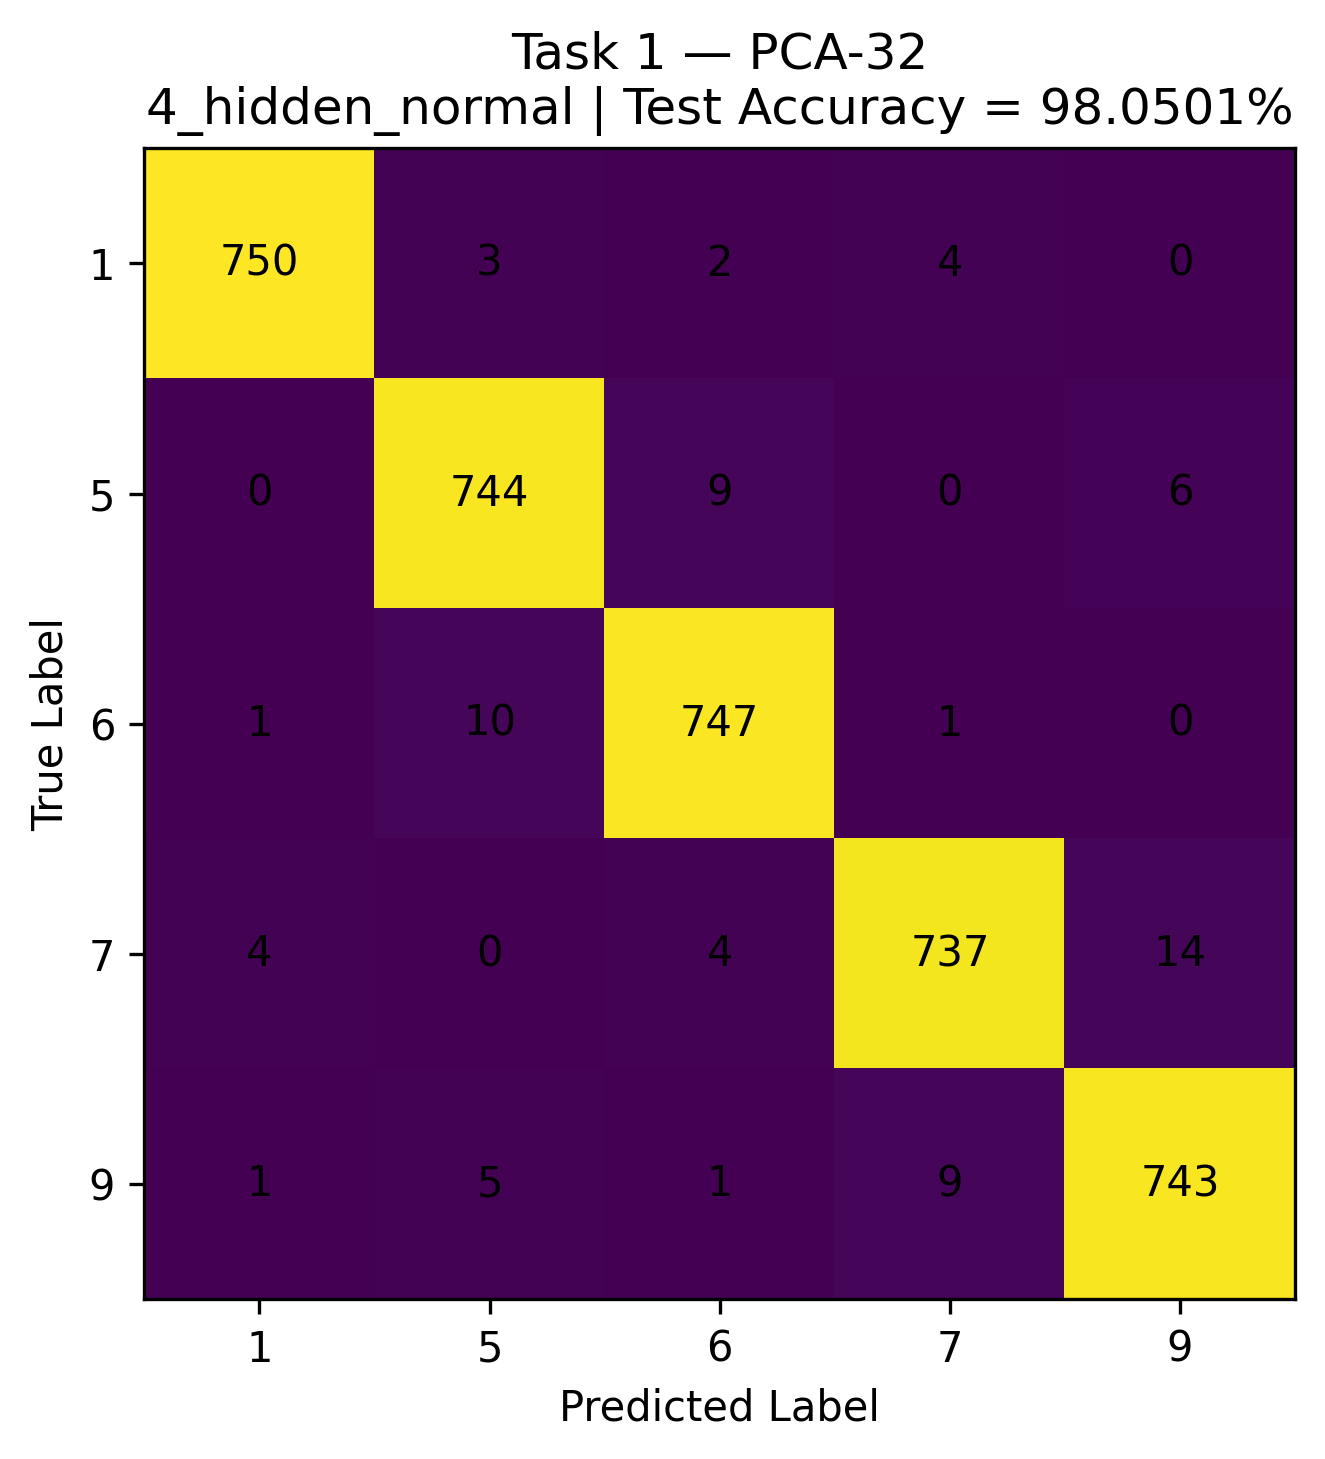
\includegraphics[width=0.88\linewidth,height=0.34\textheight,keepaspectratio]{figures/task1/cnf_mat_img/confusion_matrix_pca_32.png}
\caption{Confusion matrix: confusion matrix pca for 32 components.}
\label{fig:task1_1}
\end{figure}

\begin{figure}[H]
\centering
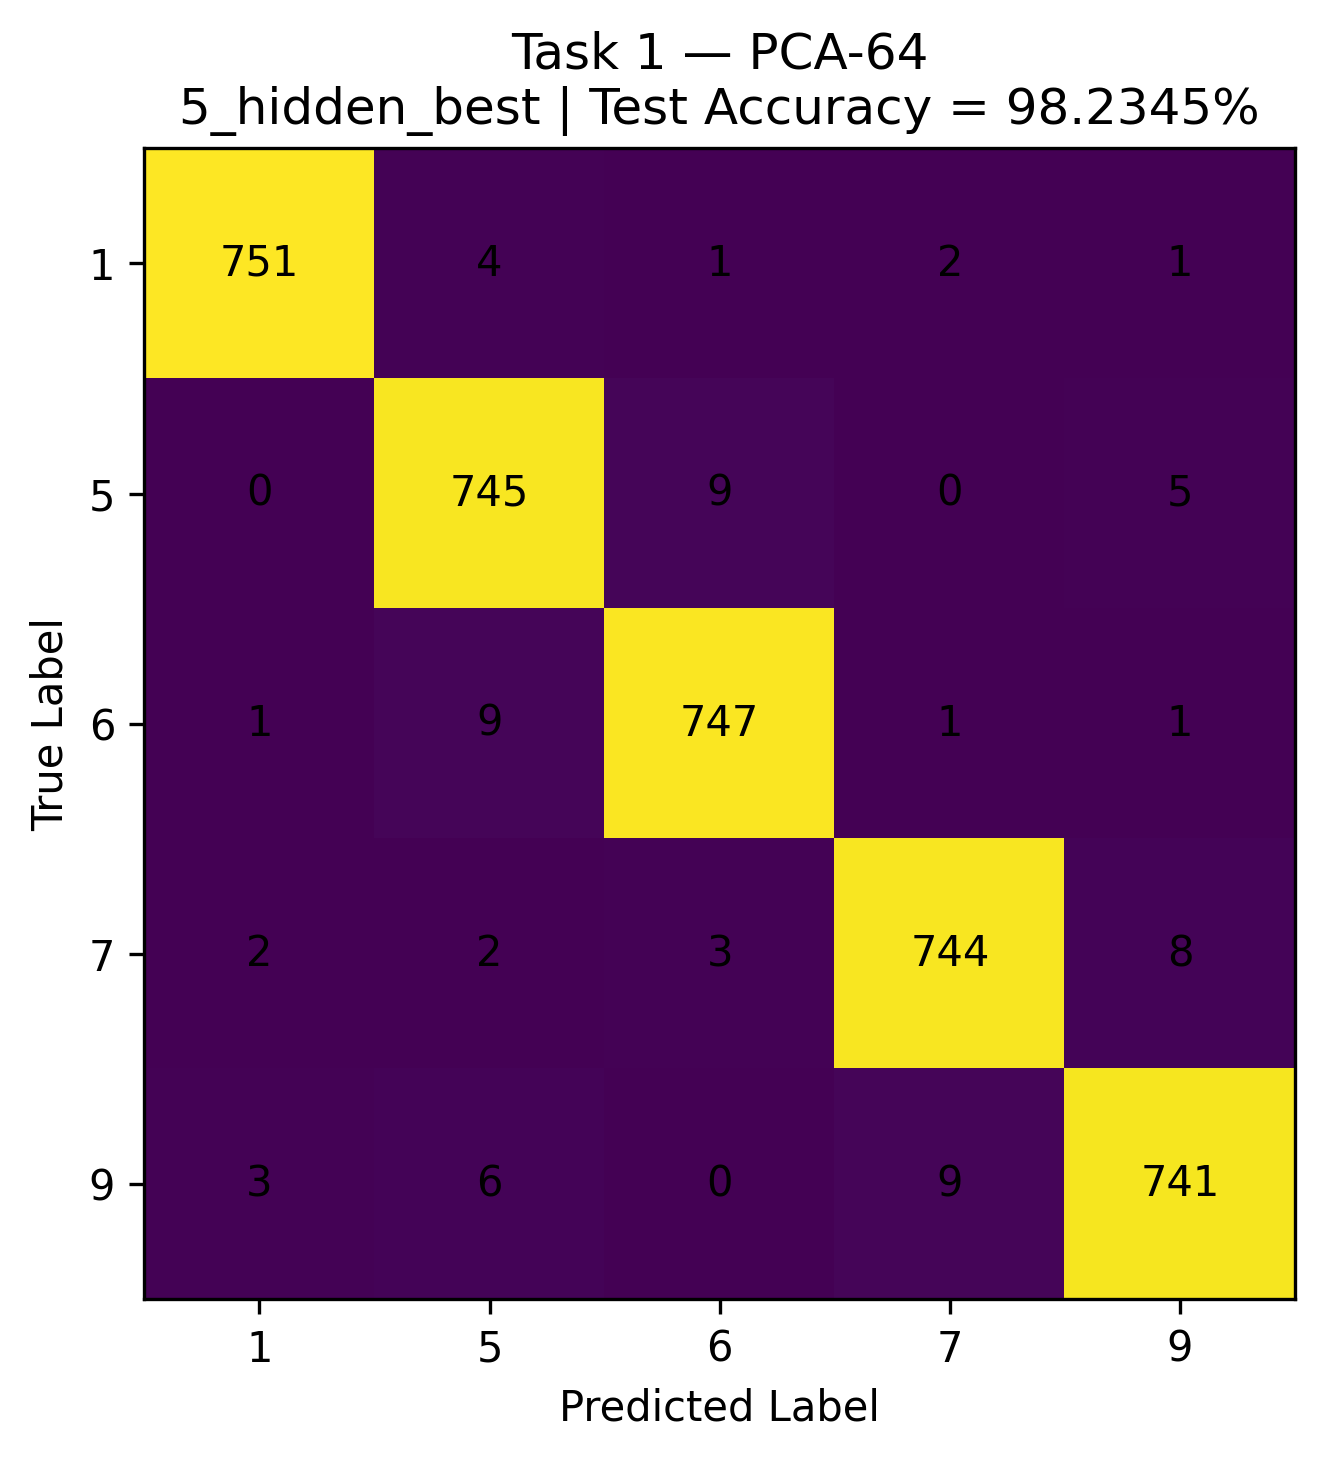
\includegraphics[width=0.88\linewidth,height=0.34\textheight,keepaspectratio]{figures/task1/cnf_mat_img/confusion_matrix_pca_64.png}
\caption{Confusion matrix: confusion matrix pca for 64 components.}
\label{fig:task1_2}
\end{figure}

\begin{figure}[H]
\centering
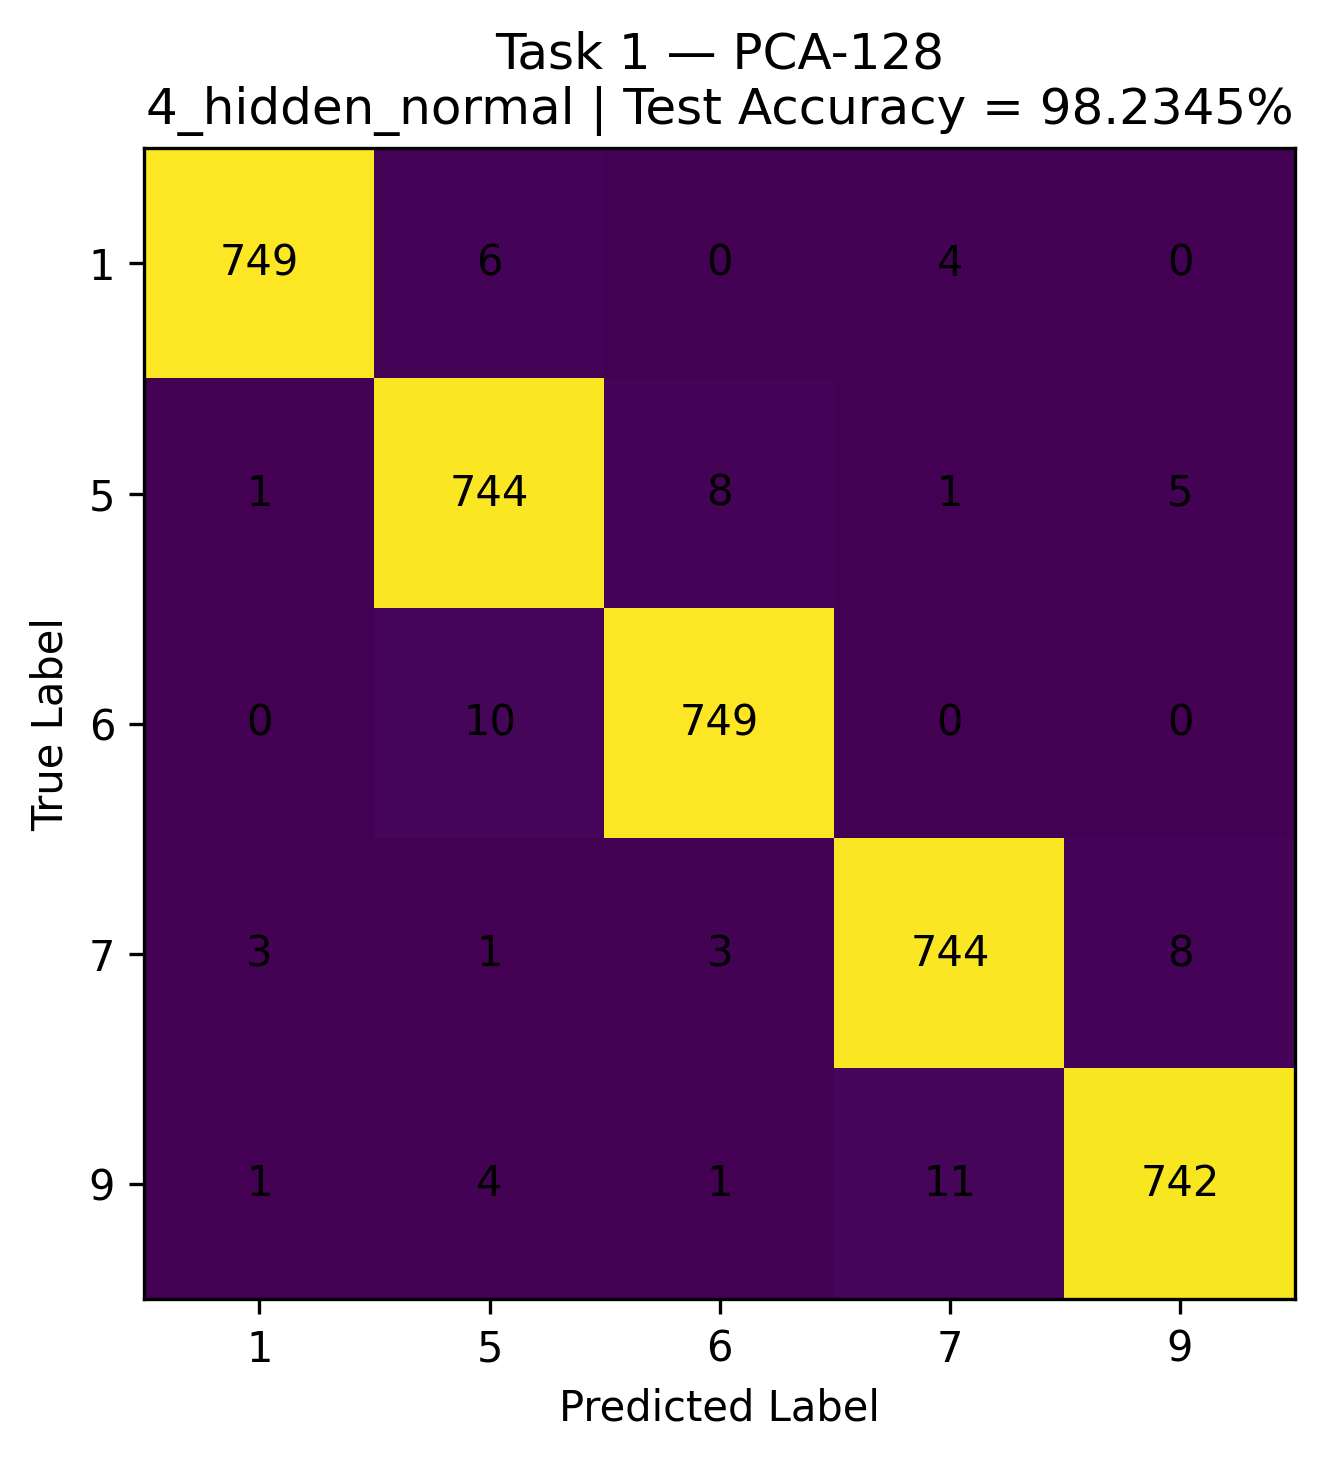
\includegraphics[width=0.88\linewidth,height=0.34\textheight,keepaspectratio]{figures/task1/cnf_mat_img/confusion_matrix_pca_128.png}
\caption{Confusion matrix: confusion matrix pca for 128 components.}
\label{fig:task1_3}
\end{figure}

\begin{figure}[H]
\centering
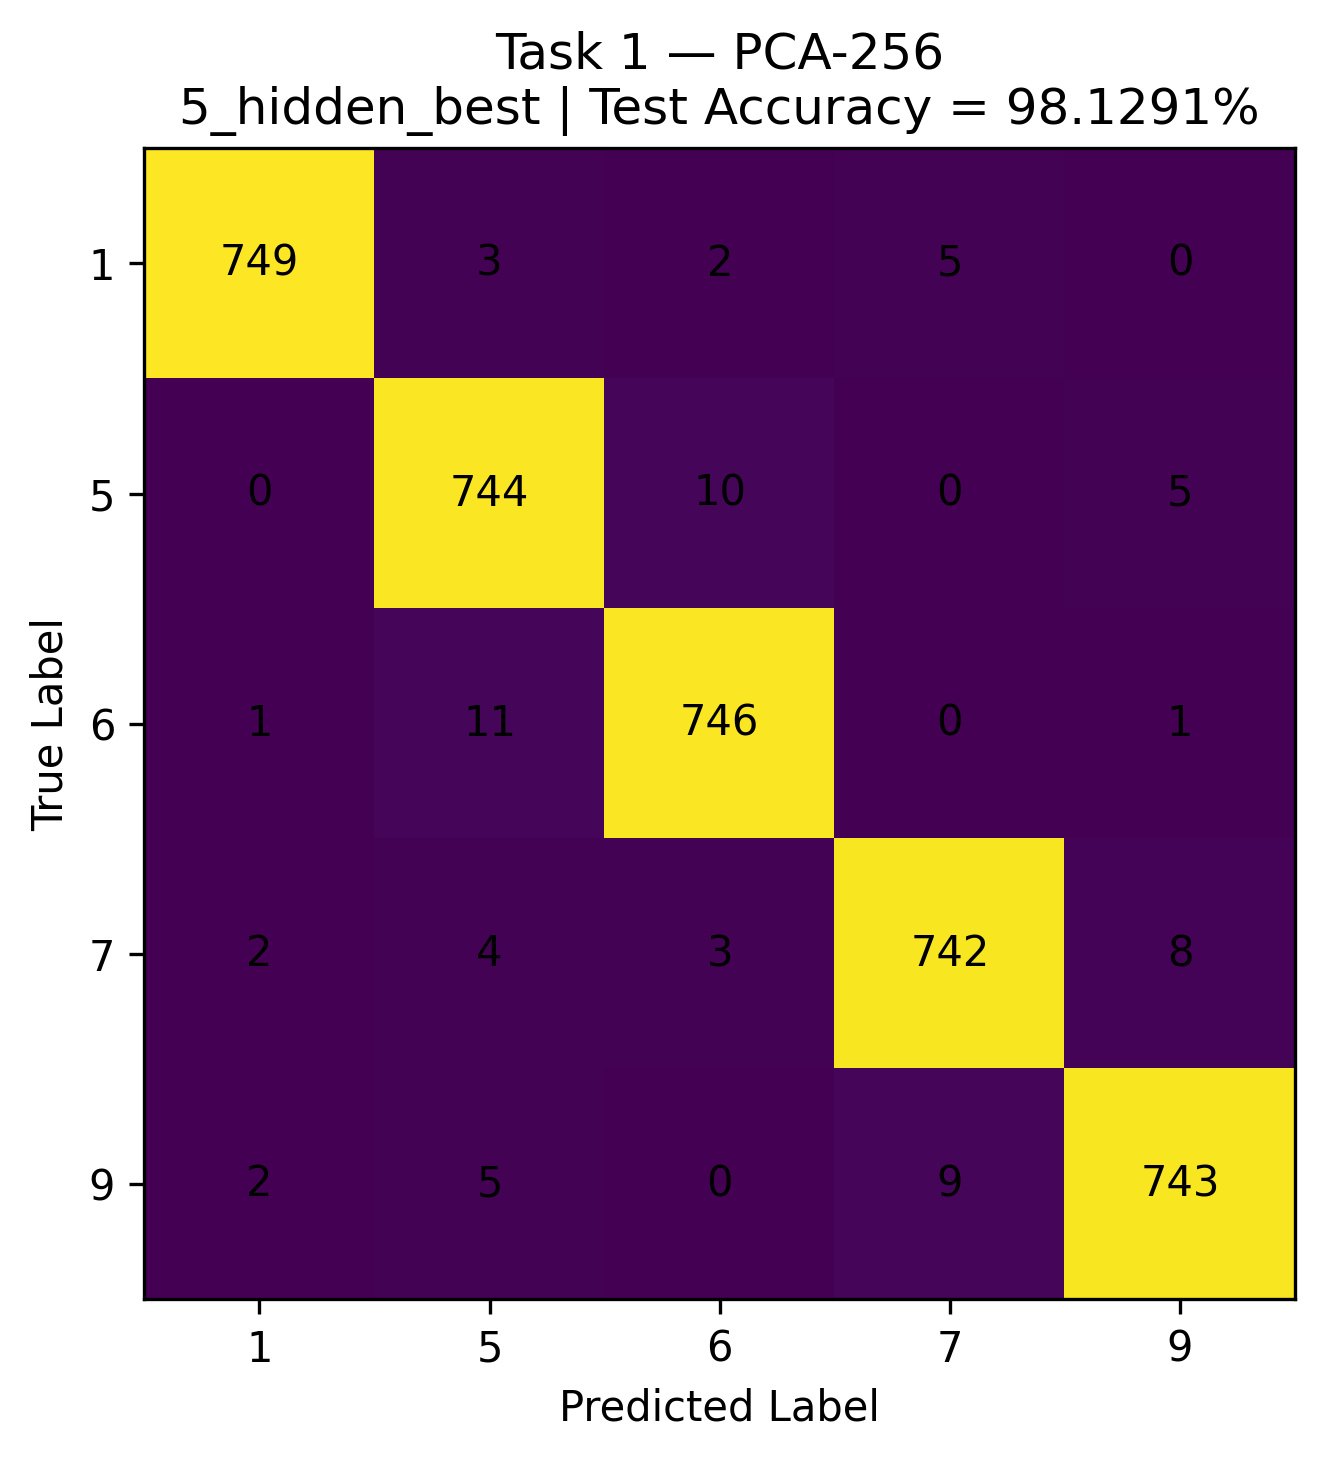
\includegraphics[width=0.88\linewidth,height=0.34\textheight,keepaspectratio]{figures/task1/cnf_mat_img/confusion_matrix_pca_256.png}
\caption{Confusion matrix: confusion matrix pca for 256 components.}
\label{fig:task1_4}
\end{figure}

\FloatBarrier

\section{Task 2: Autoencoder Reconstruction}
\subsection{Architectures and training}
Two autoencoder(AE) families are evaluated at bottleneck dimensions 32, 64, 128, and 256. The one-hidden-layer model maps the 784-dimensional input directly to the bottleneck and then reconstructs the input. The three-hidden-layer model uses the architecture $784\rightarrow400\rightarrow d\rightarrow400\rightarrow784$, where $d$ is the bottleneck dimension. The one-hidden-layer encoder and decoder use logistic activations except for the linear
bottleneck; the decoder output also uses logistic so that reconstructed pixels remain in
$[0,1]$. In the three-hidden-layer model, both 400-unit hidden layers use logistic activation,
the bottleneck is linear, and the output layer uses logistic. Both families are optimized
with Adam at learning rate $0.001$ for 500 epochs. The supplied final results correspond to the 500-epoch runs. Reconstruction error is evaluated separately on training, validation, and test data.

\subsection{Quantitative results}
Table~\ref{tab:ae-mse} reports train, validation, and test reconstruction MSE for all eight trained autoencoders. For the one-hidden-layer autoencoder, test MSE decreases as the bottleneck grows from 32 to 256 dimensions. The three-hidden-layer model also improves between 32 and 256 dimensions, although its MSE is not lower than the one-hidden-layer model at every dimension. This illustrates that reconstruction quality depends on both bottleneck capacity and architecture rather than depth alone.

\begin{table}[H]
\centering
\small
\caption{Reconstruction MSE on training, validation, and test sets after the selected 500-epoch runs.}
\label{tab:ae-mse}
\begin{tabular}{r l r r r}
\toprule
Bottleneck & Architecture & Train MSE & Validation MSE & Test MSE\\
\midrule
32 & One-hidden AE & 0.006452 & 0.007211 & 0.007314 \\
64 & One-hidden AE & 0.002369 & 0.003019 & 0.003065 \\
128 & One-hidden AE & 0.000953 & 0.001416 & 0.001415 \\
256 & One-hidden AE & 0.000498 & 0.000805 & 0.000805 \\
32 & Three-hidden AE & 0.002815 & 0.005041 & 0.005136 \\
64 & Three-hidden AE & 0.001463 & 0.003398 & 0.003467 \\
128 & Three-hidden AE & 0.000761 & 0.002209 & 0.002226 \\
256 & Three-hidden AE & 0.000582 & 0.001576 & 0.001588 \\
\bottomrule
\end{tabular}
\end{table}

The following figures preserve the supplied reconstruction examples for the training, validation, and test splits. These visualizations allow the reconstructed strokes and class-specific distortions to be inspected alongside the numerical MSE values.

% Automatically generated figure inventory for task2.

\begin{figure}[H]
\centering
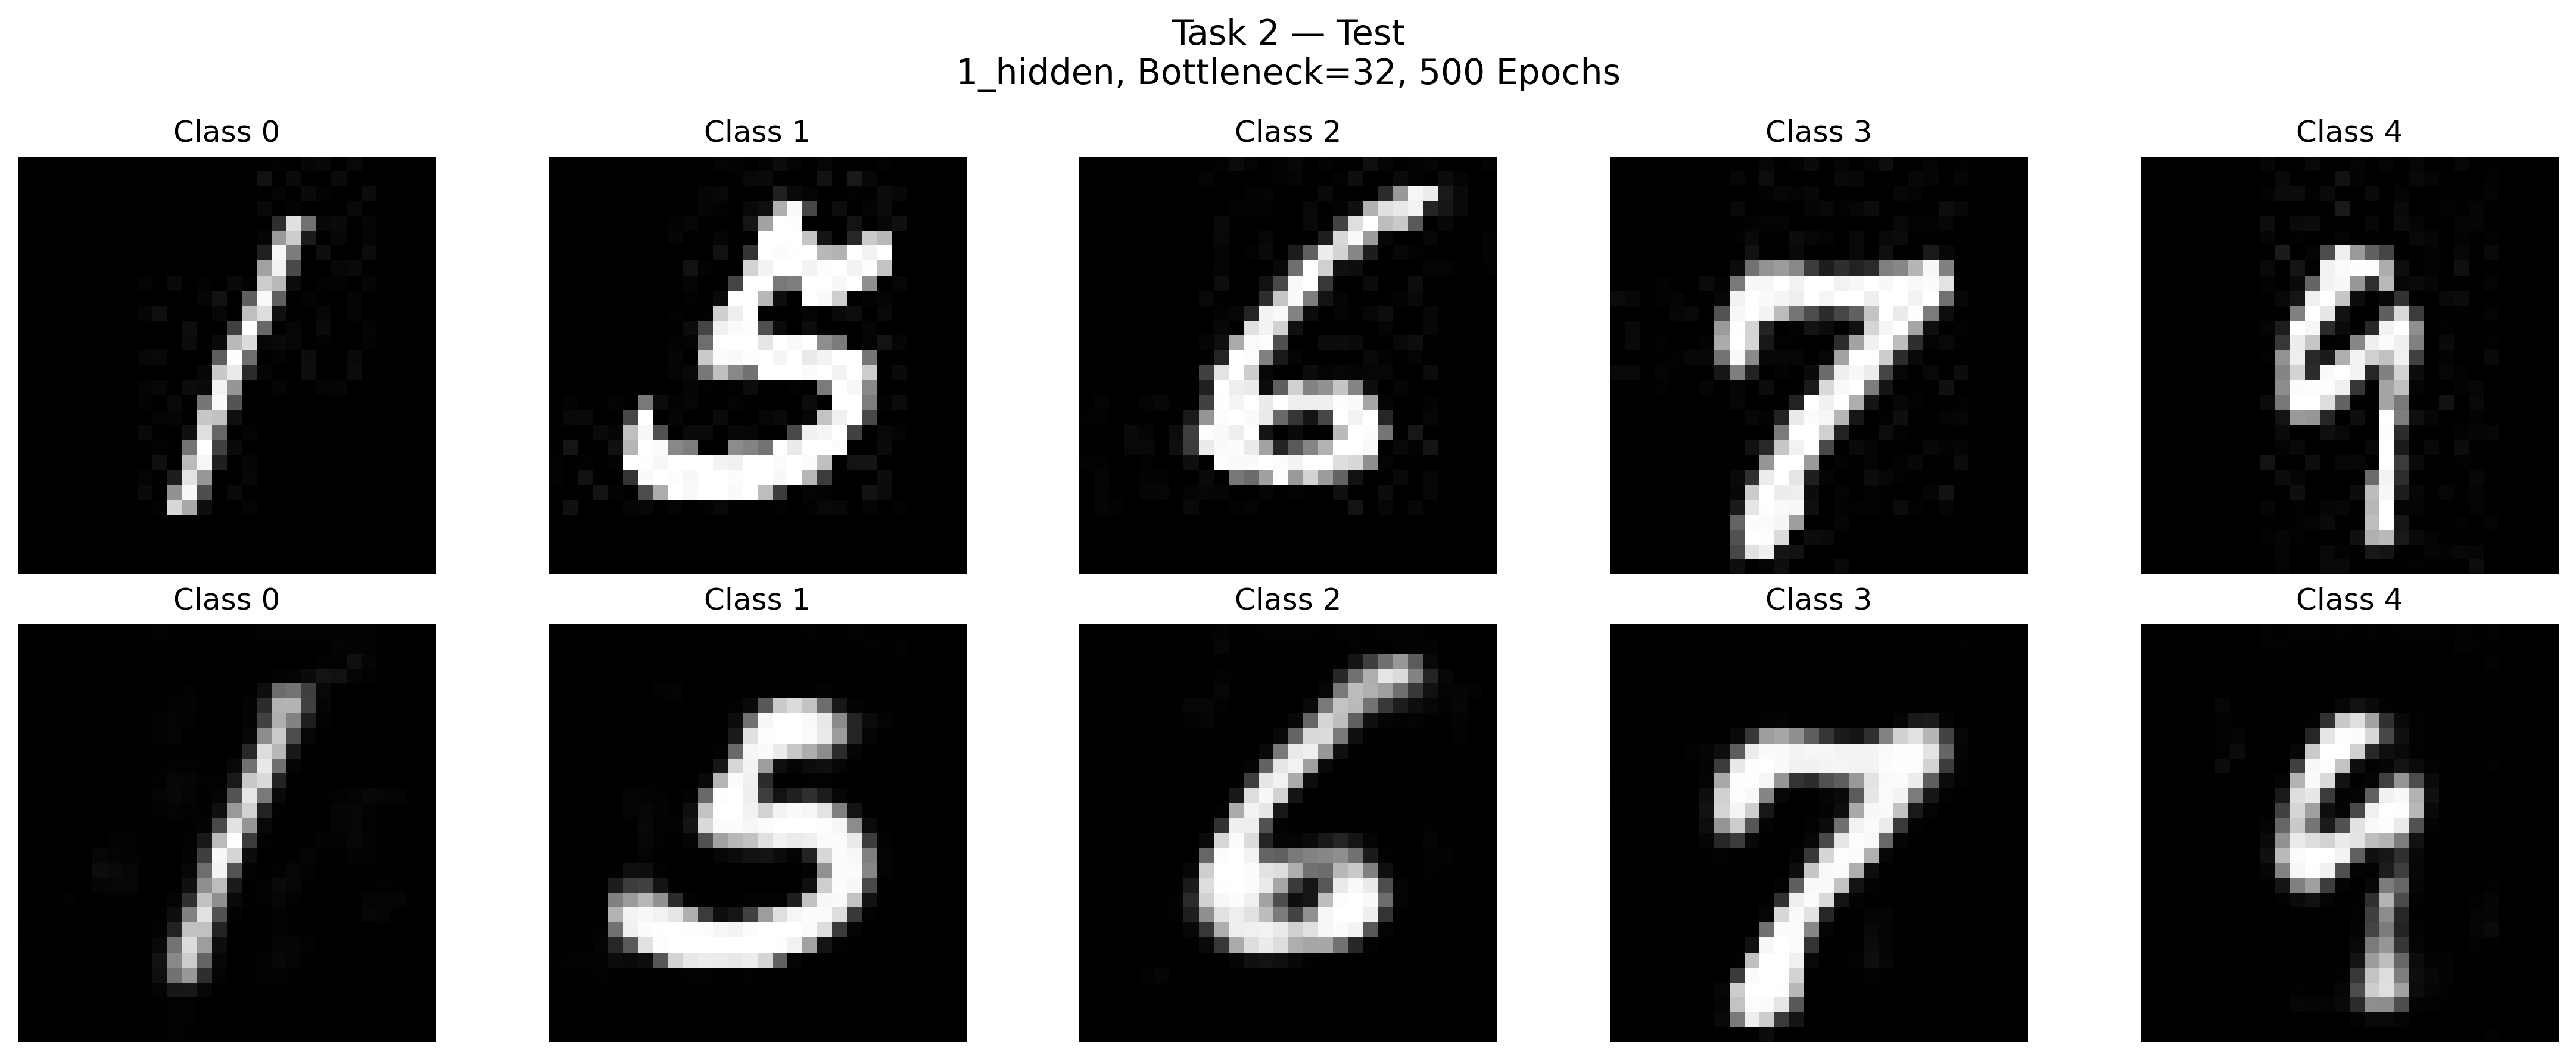
\includegraphics[width=0.96\linewidth,height=0.48\textheight,keepaspectratio]{figures/task2/model_reconstruction_visualization_500/test_1_hidden_bottleneck_32_500epochs.png}
\caption{Autoencoder reconstruction visualization: test 1 hidden with bottleneck of 32 neurons.}
\label{fig:task2_1}
\end{figure}

\begin{figure}[H]
\centering
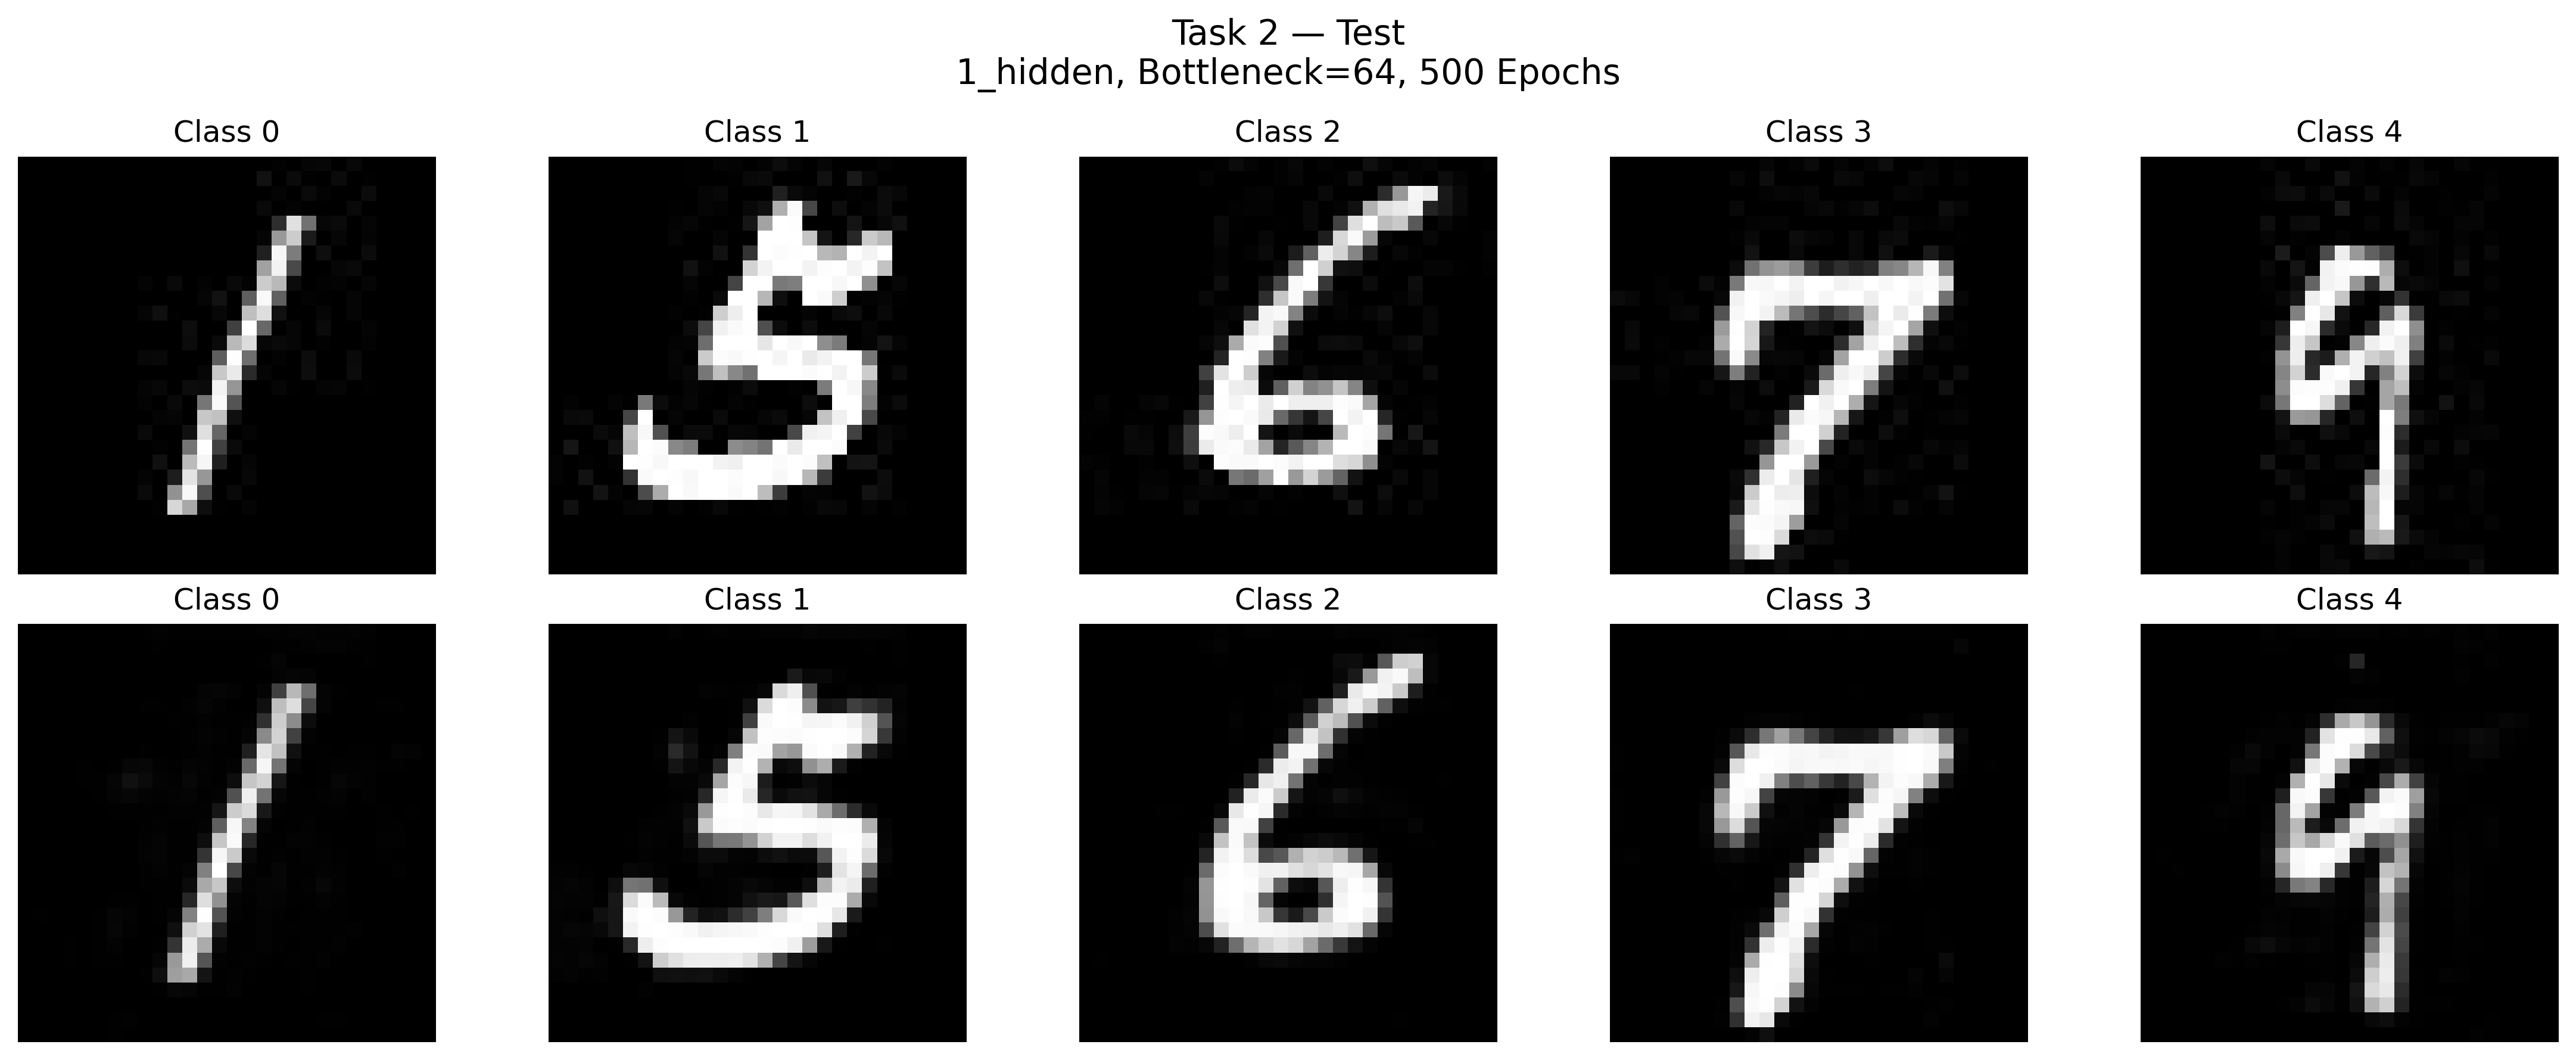
\includegraphics[width=0.96\linewidth,height=0.48\textheight,keepaspectratio]{figures/task2/model_reconstruction_visualization_500/test_1_hidden_bottleneck_64_500epochs.png}
\caption{Autoencoder reconstruction visualization: test 1 hidden with bottleneck of 64 neurons.}
\label{fig:task2_2}
\end{figure}

\begin{figure}[H]
\centering
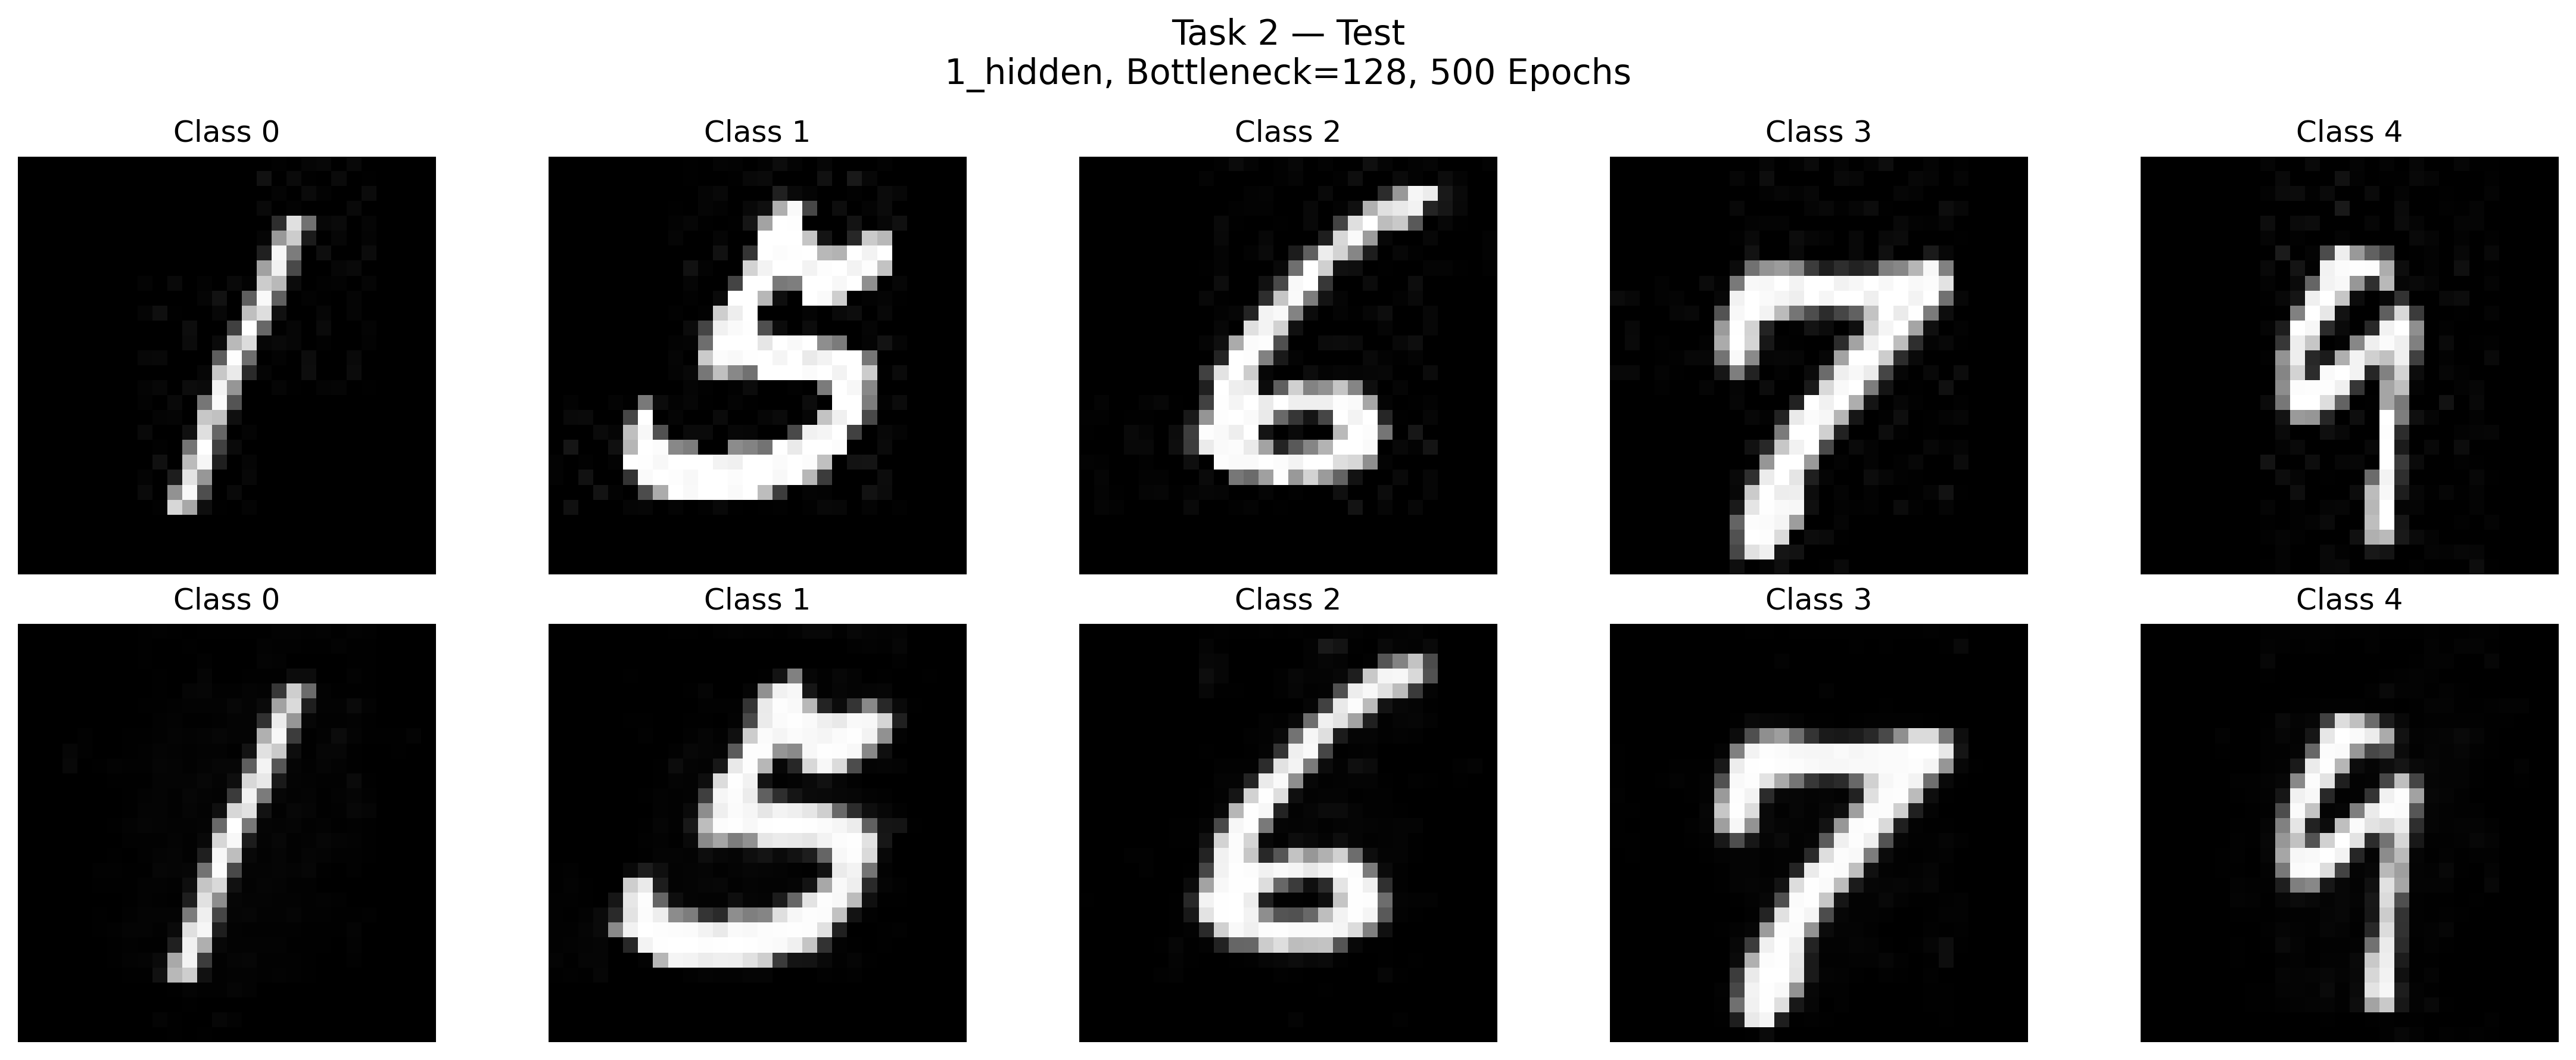
\includegraphics[width=0.96\linewidth,height=0.48\textheight,keepaspectratio]{figures/task2/model_reconstruction_visualization_500/test_1_hidden_bottleneck_128_500epochs.png}
\caption{Autoencoder reconstruction visualization: test 1 hidden with bottleneck of 128 neurons.}
\label{fig:task2_3}
\end{figure}

\begin{figure}[H]
\centering
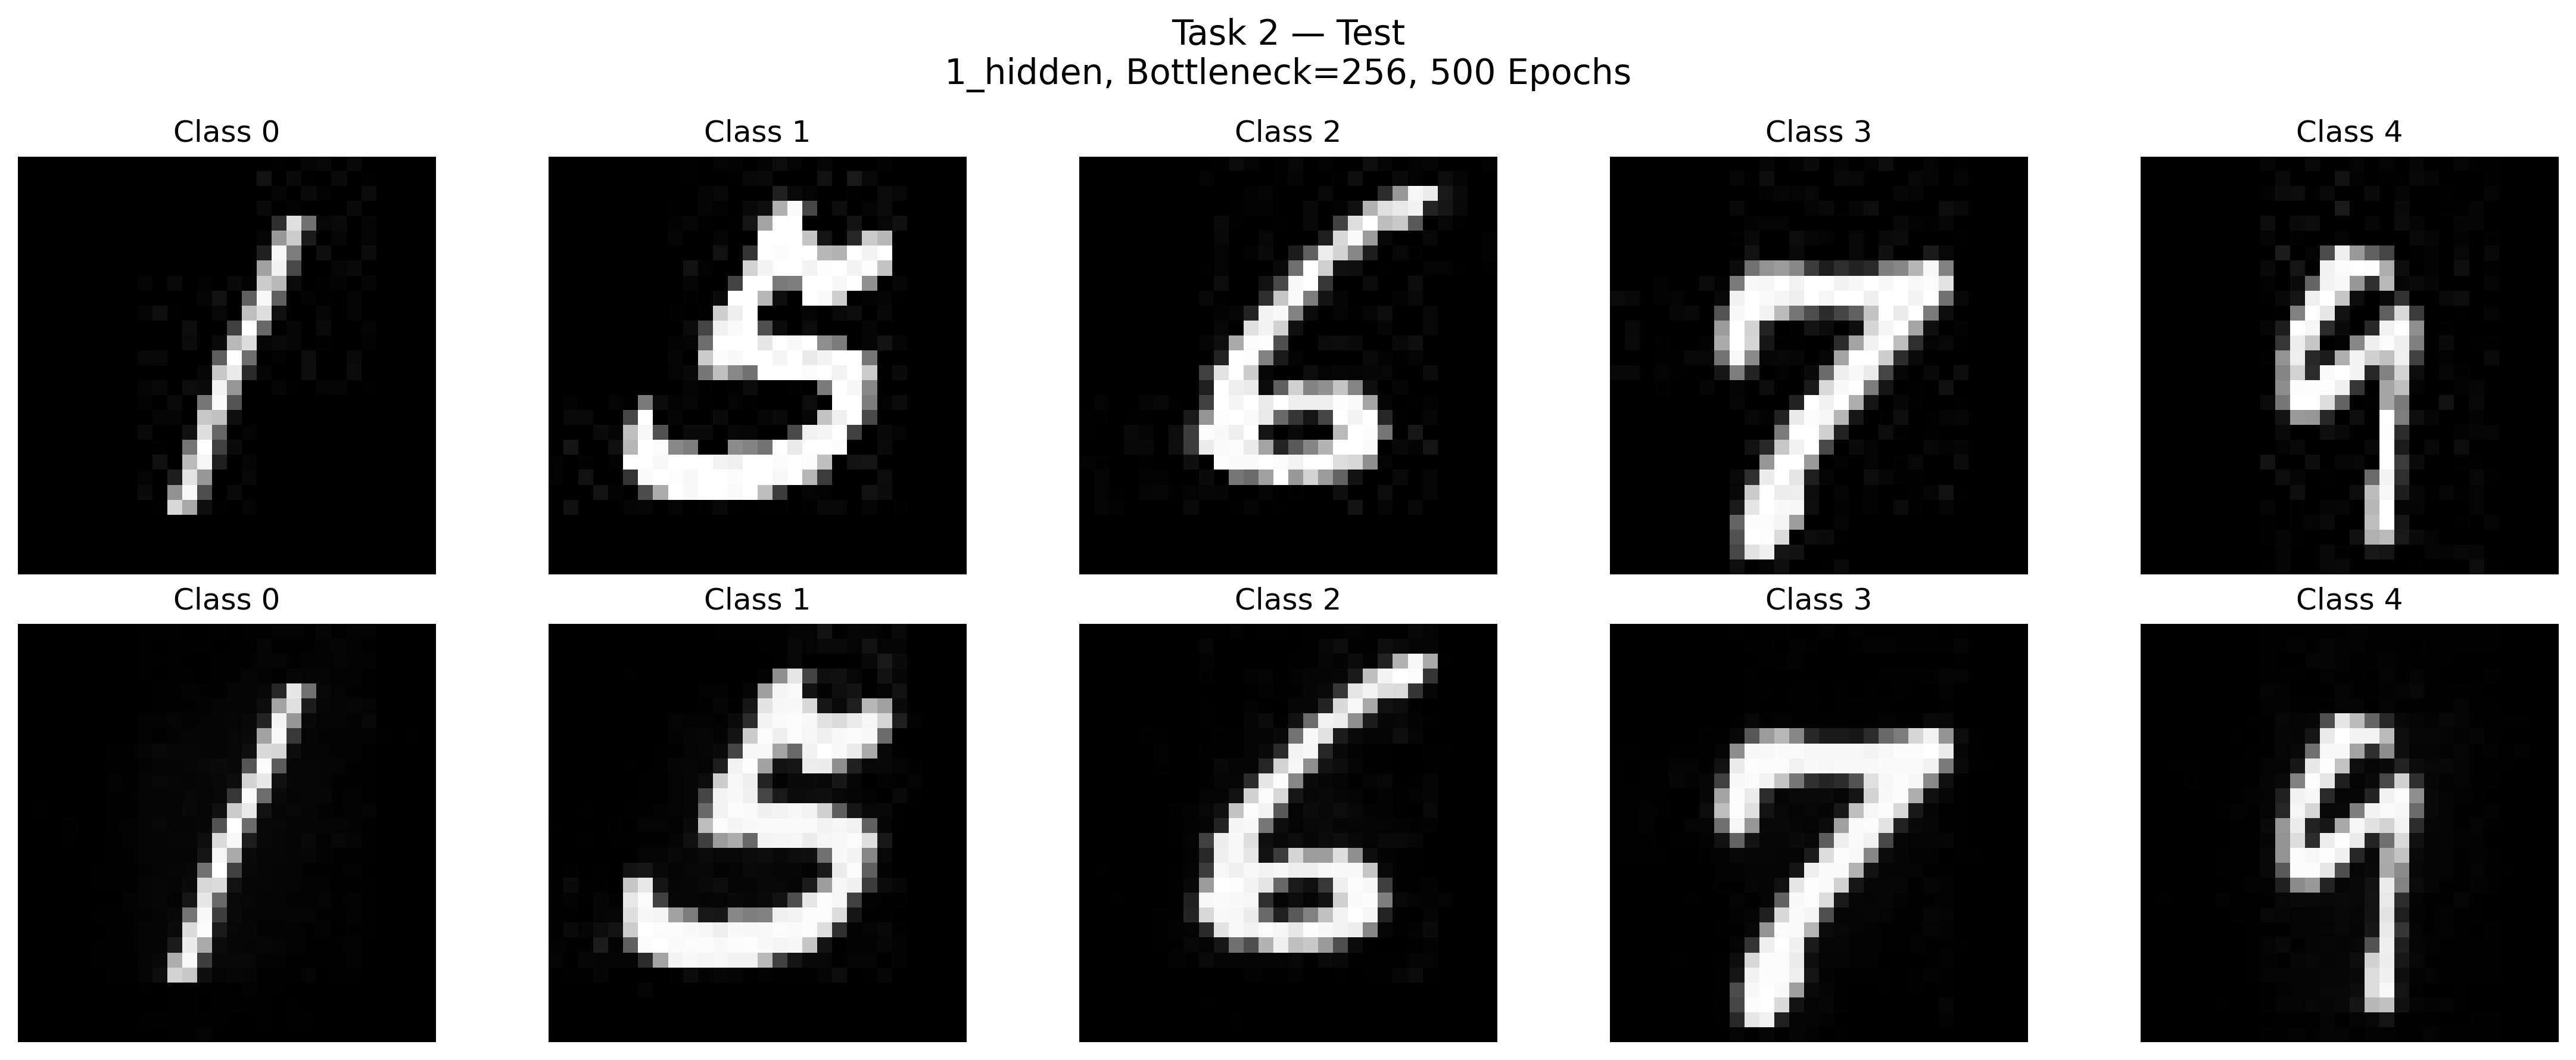
\includegraphics[width=0.96\linewidth,height=0.48\textheight,keepaspectratio]{figures/task2/model_reconstruction_visualization_500/test_1_hidden_bottleneck_256_500epochs.png}
\caption{Autoencoder reconstruction visualization: test 1 hidden with bottleneck of 256 neurons.}
\label{fig:task2_4}
\end{figure}

\begin{figure}[H]
\centering
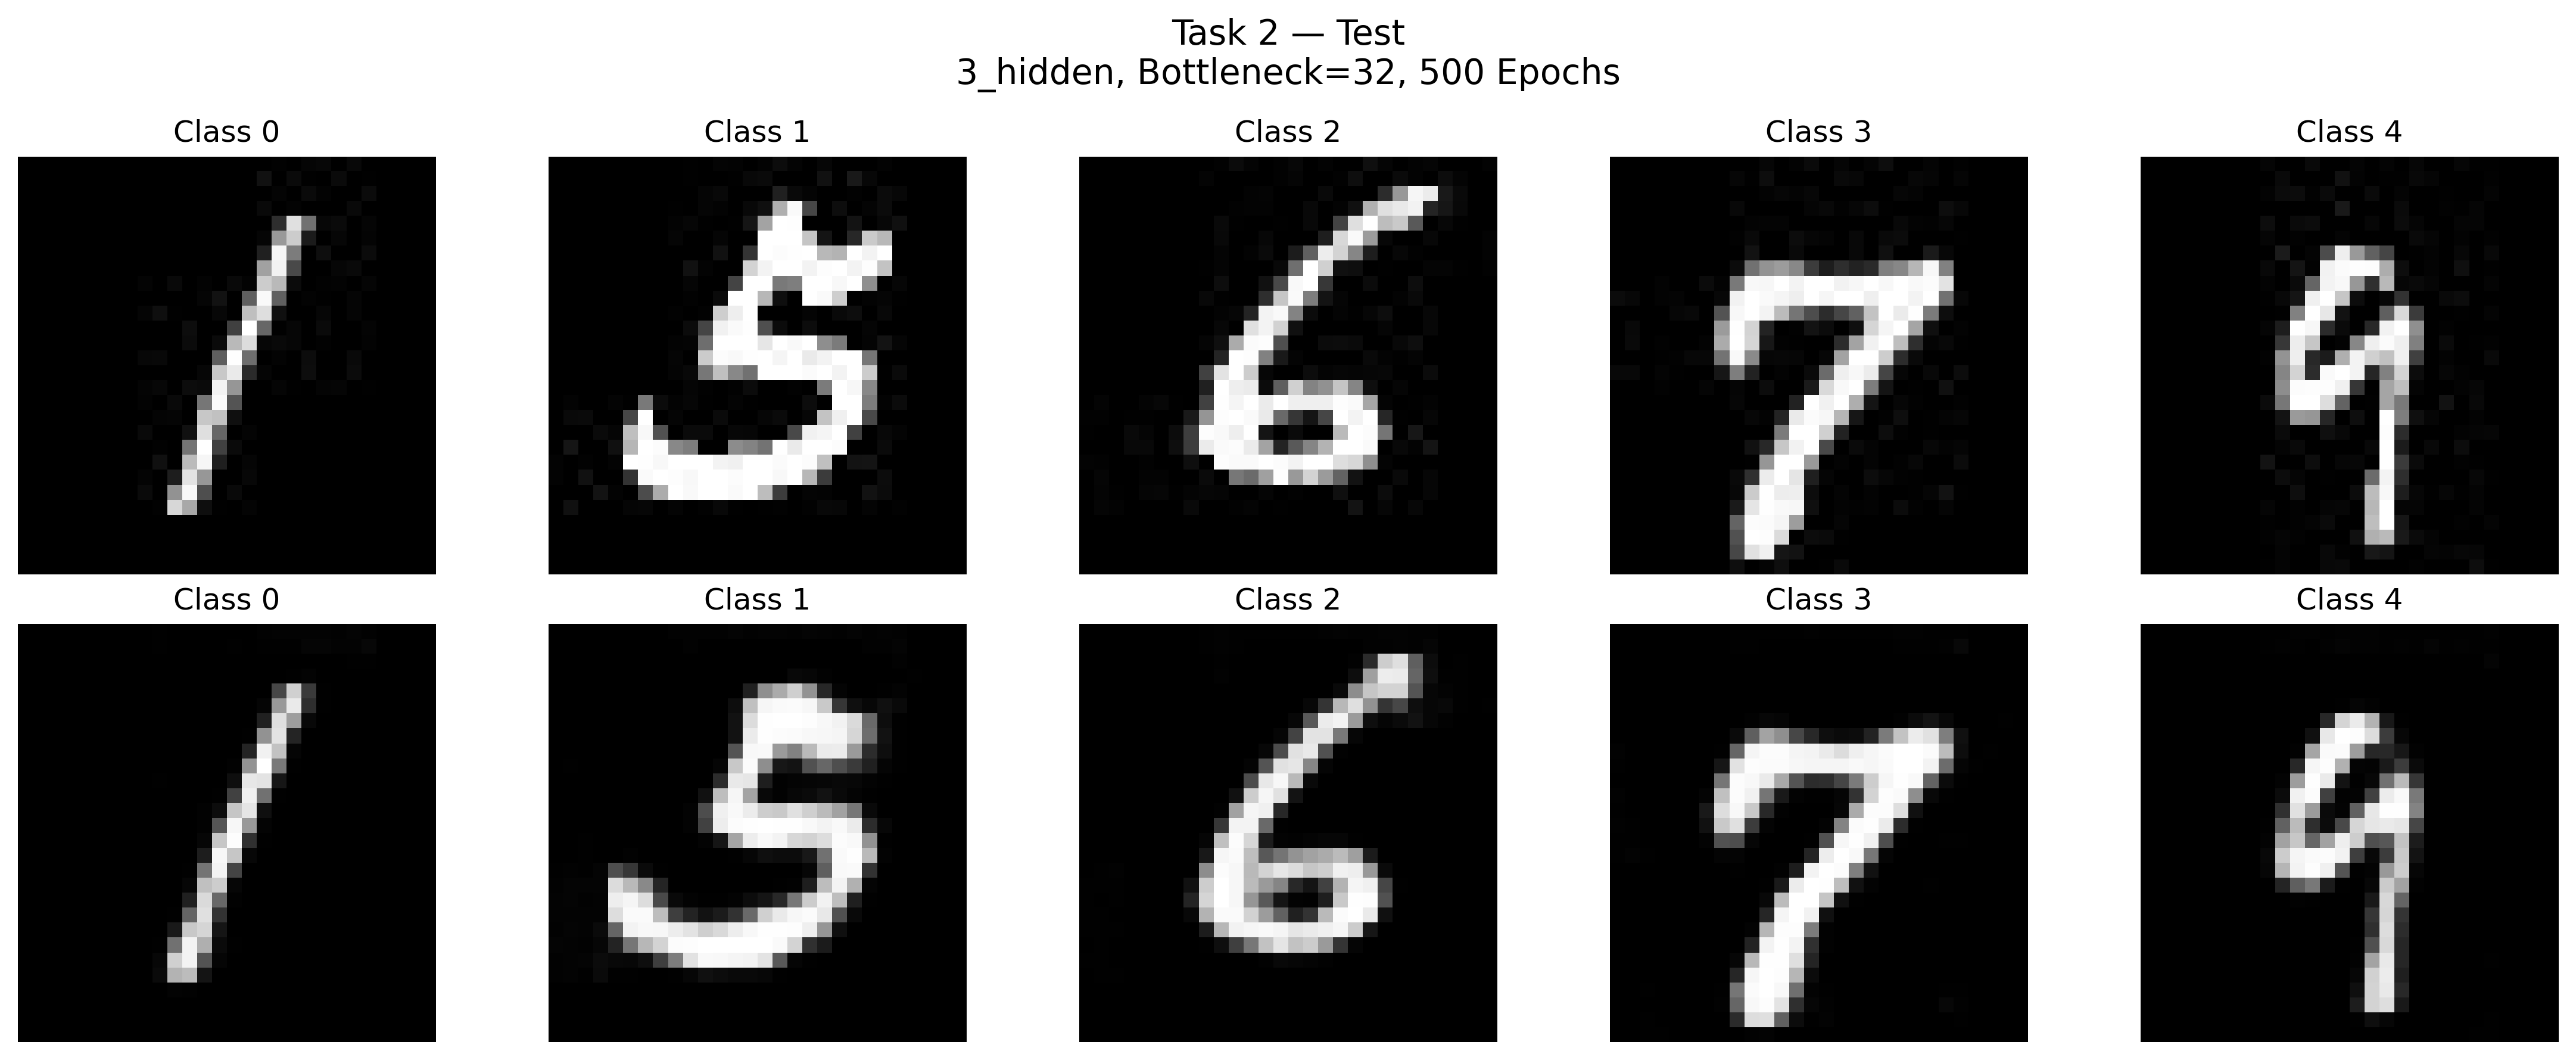
\includegraphics[width=0.96\linewidth,height=0.48\textheight,keepaspectratio]{figures/task2/model_reconstruction_visualization_500/test_3_hidden_bottleneck_32_500epochs.png}
\caption{Autoencoder reconstruction visualization: test 3 hidden with bottleneck of 32 neurons.}
\label{fig:task2_5}
\end{figure}

\begin{figure}[H]
\centering
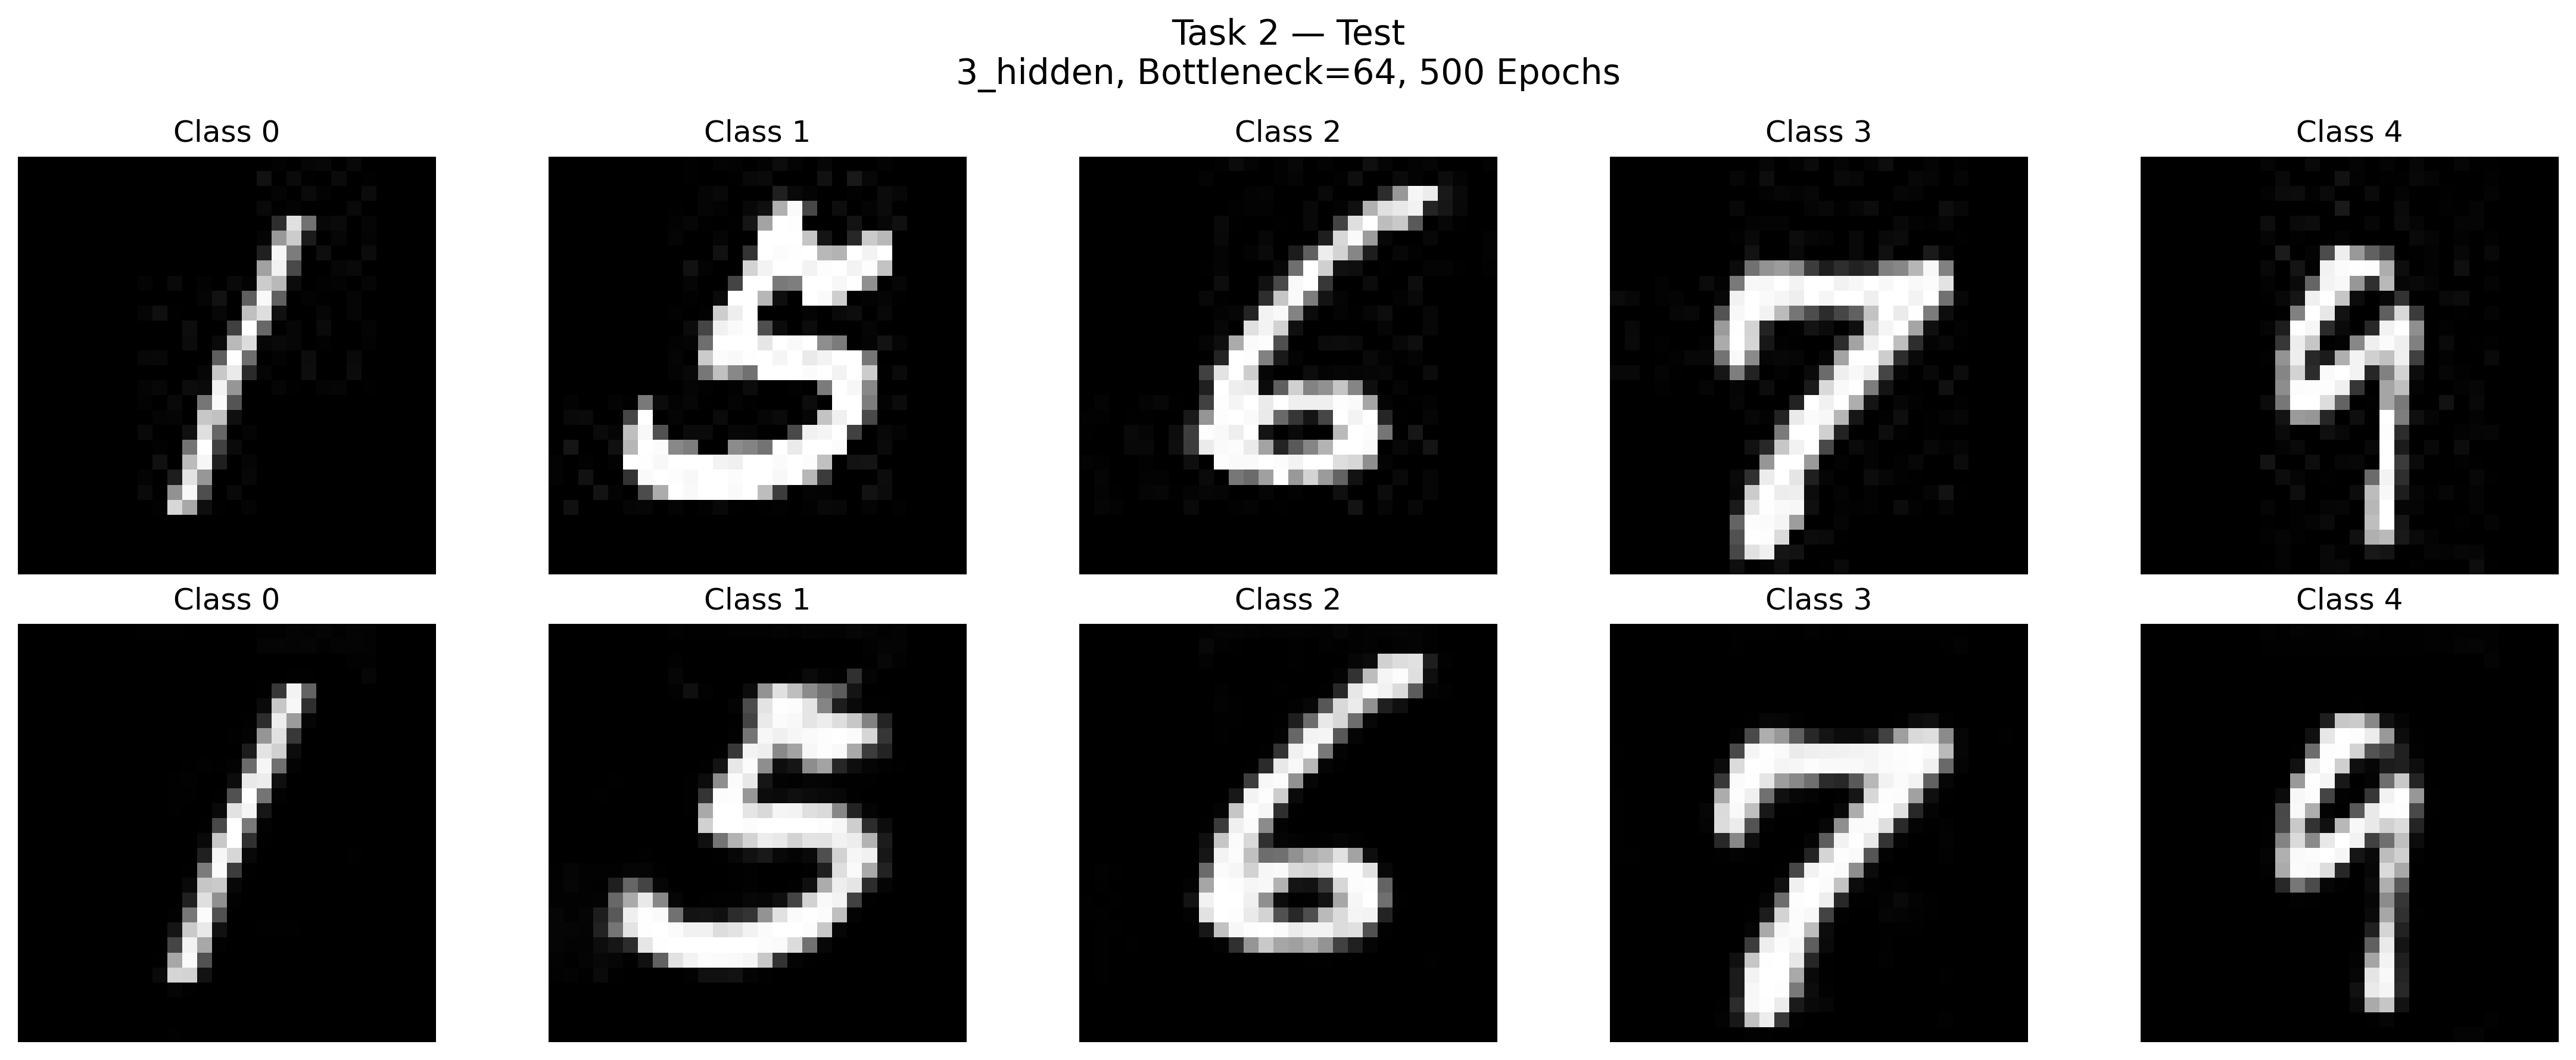
\includegraphics[width=0.96\linewidth,height=0.48\textheight,keepaspectratio]{figures/task2/model_reconstruction_visualization_500/test_3_hidden_bottleneck_64_500epochs.png}
\caption{Autoencoder reconstruction visualization: test 3 hidden with bottleneck of 64 neurons.}
\label{fig:task2_6}
\end{figure}

\begin{figure}[H]
\centering
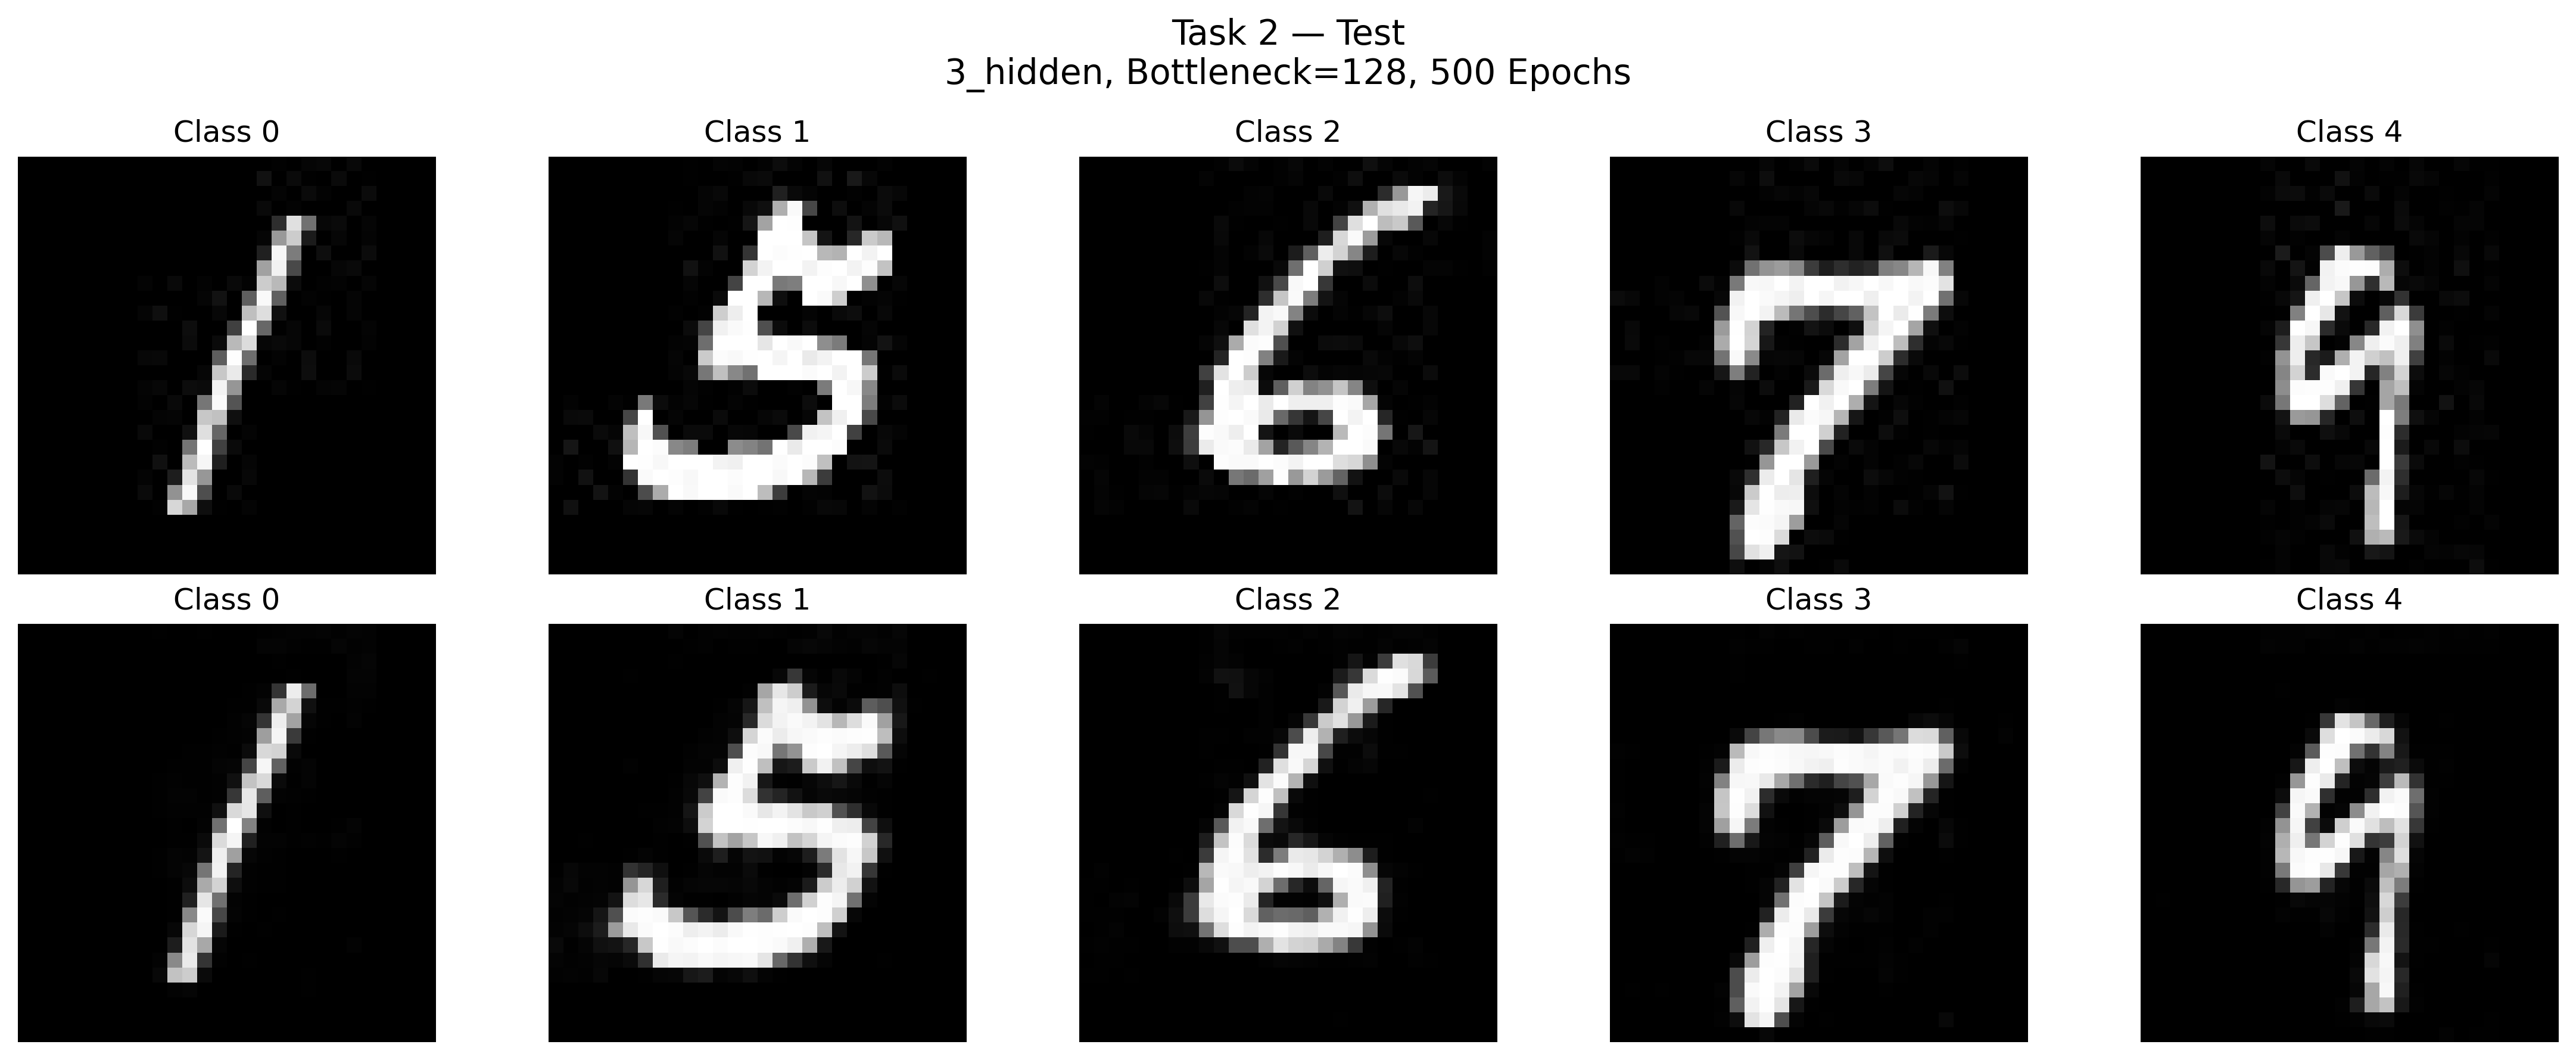
\includegraphics[width=0.96\linewidth,height=0.48\textheight,keepaspectratio]{figures/task2/model_reconstruction_visualization_500/test_3_hidden_bottleneck_128_500epochs.png}
\caption{Autoencoder reconstruction visualization: test 3 hidden with bottleneck of 128 neurons.}
\label{fig:task2_7}
\end{figure}

\begin{figure}[H]
\centering
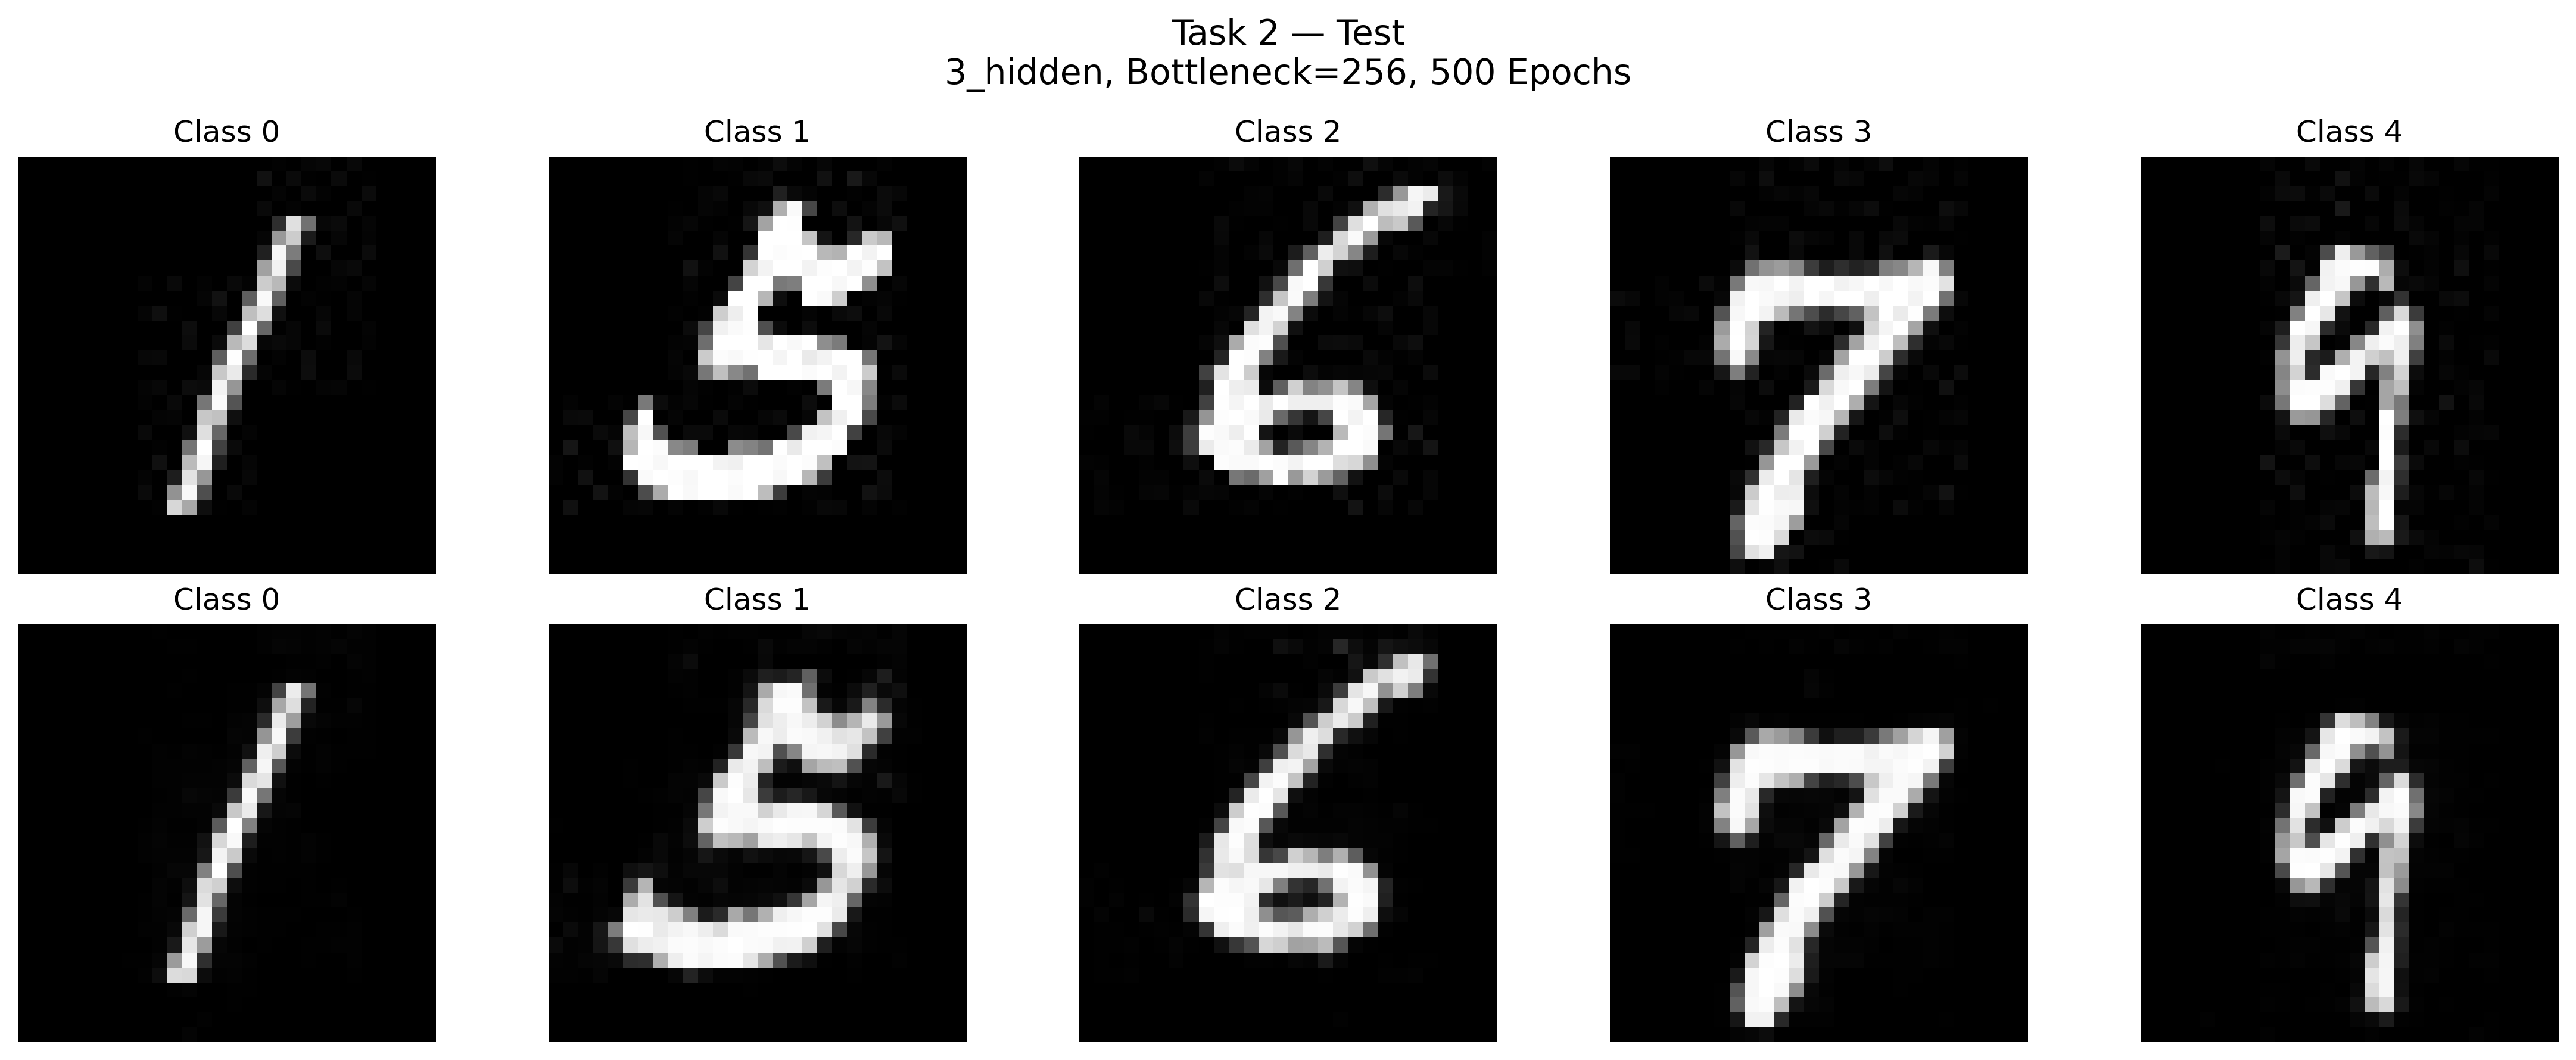
\includegraphics[width=0.96\linewidth,height=0.48\textheight,keepaspectratio]{figures/task2/model_reconstruction_visualization_500/test_3_hidden_bottleneck_256_500epochs.png}
\caption{Autoencoder reconstruction visualization: test 3 hidden with bottleneck of 256 neurons.}
\label{fig:task2_8}
\end{figure}

\begin{figure}[H]
\centering
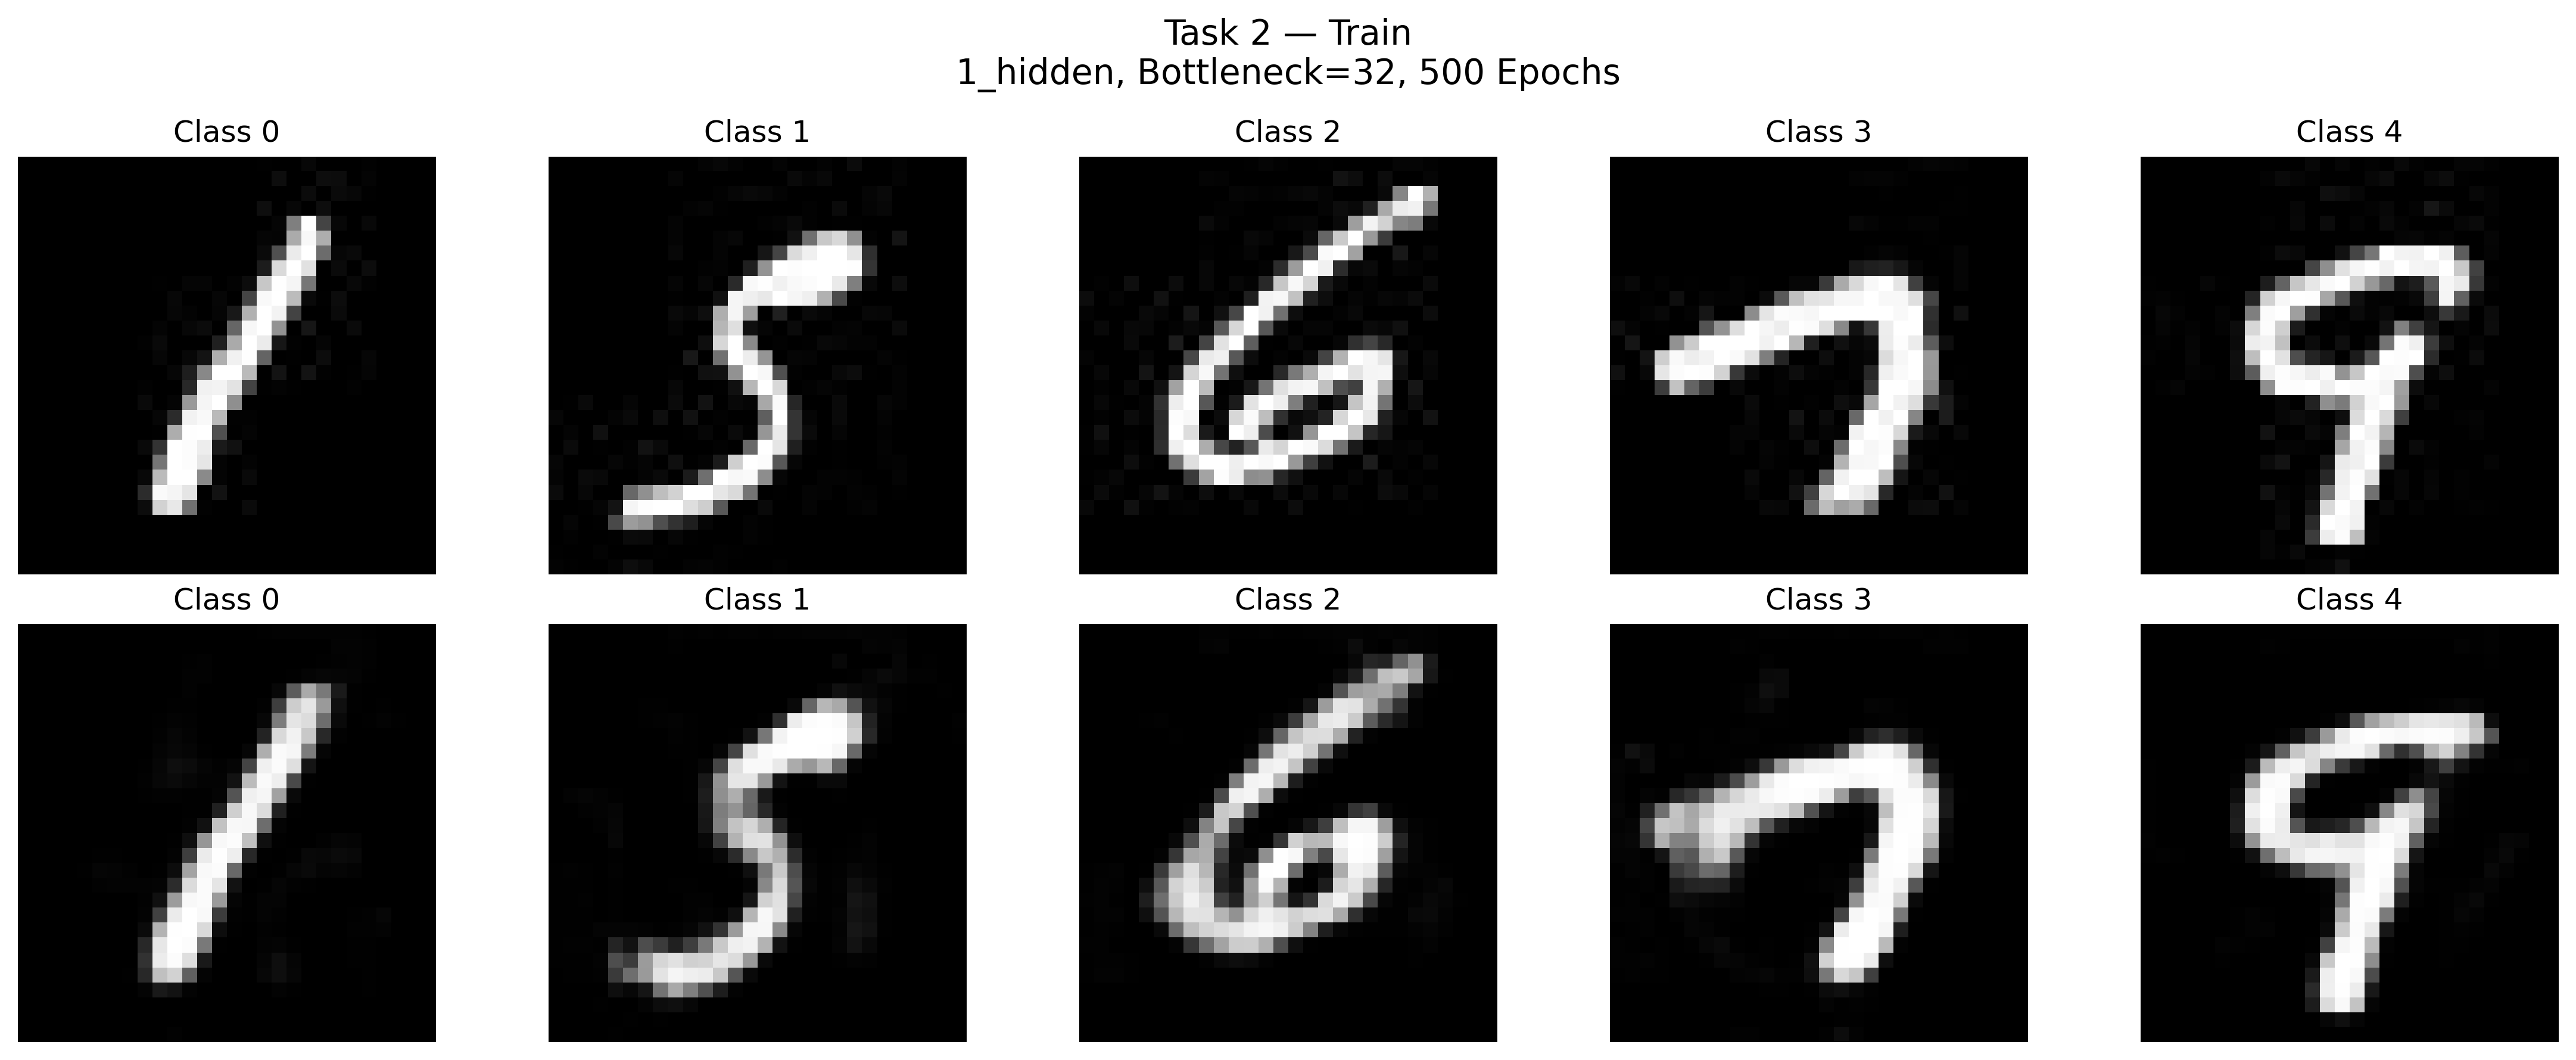
\includegraphics[width=0.96\linewidth,height=0.48\textheight,keepaspectratio]{figures/task2/model_reconstruction_visualization_500/train_1_hidden_bottleneck_32_500epochs.png}
\caption{Autoencoder reconstruction visualization: train 1 hidden with bottleneck of 32 neurons.}
\label{fig:task2_9}
\end{figure}

\begin{figure}[H]
\centering
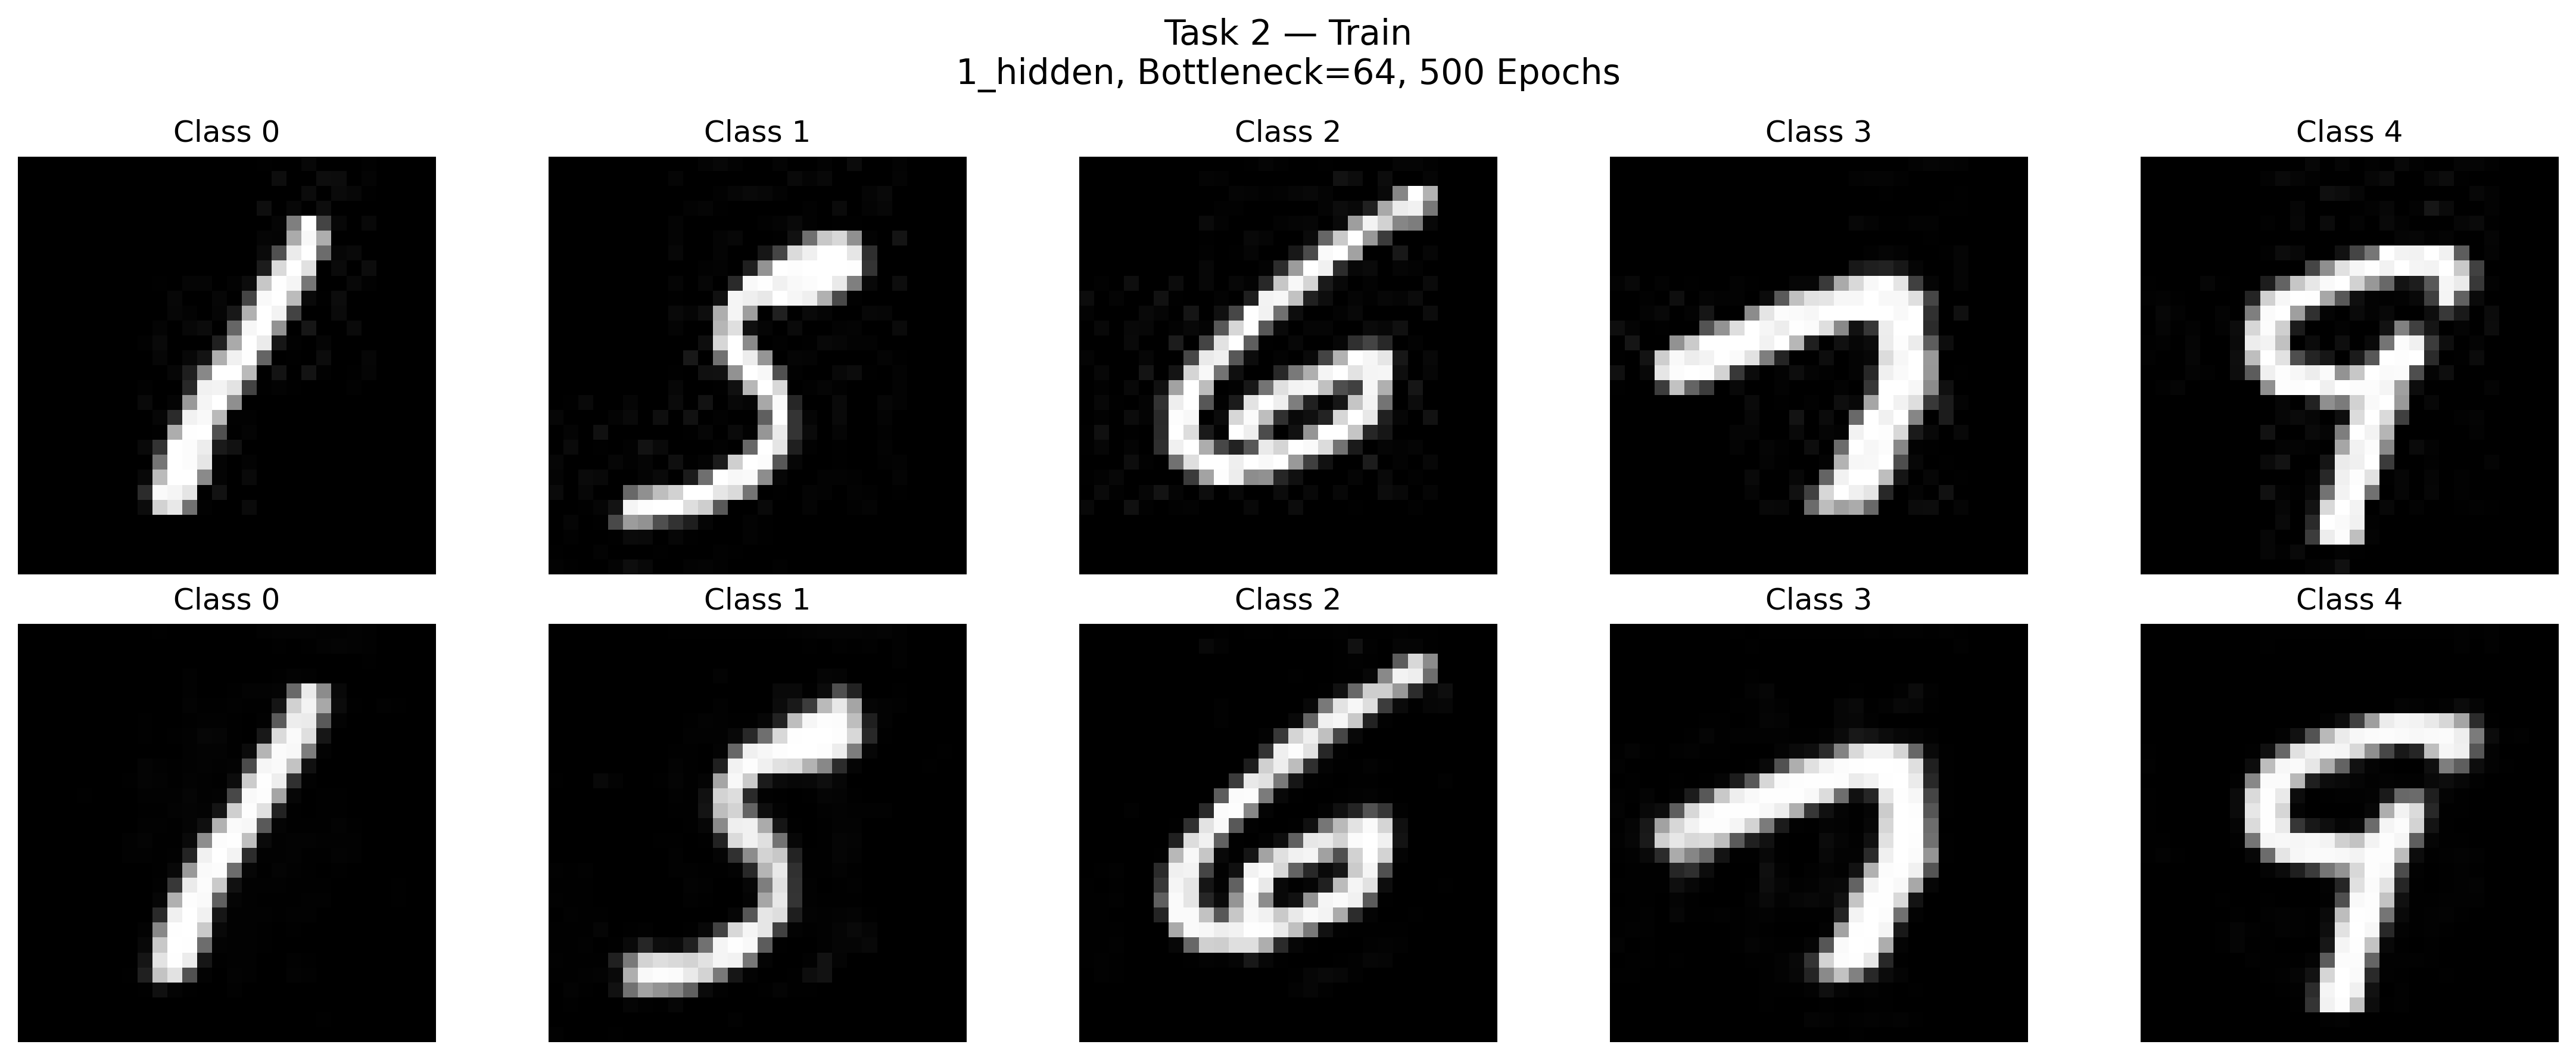
\includegraphics[width=0.96\linewidth,height=0.48\textheight,keepaspectratio]{figures/task2/model_reconstruction_visualization_500/train_1_hidden_bottleneck_64_500epochs.png}
\caption{Autoencoder reconstruction visualization: train 1 hidden with bottleneck of 64 neurons.}
\label{fig:task2_10}
\end{figure}

\begin{figure}[H]
\centering
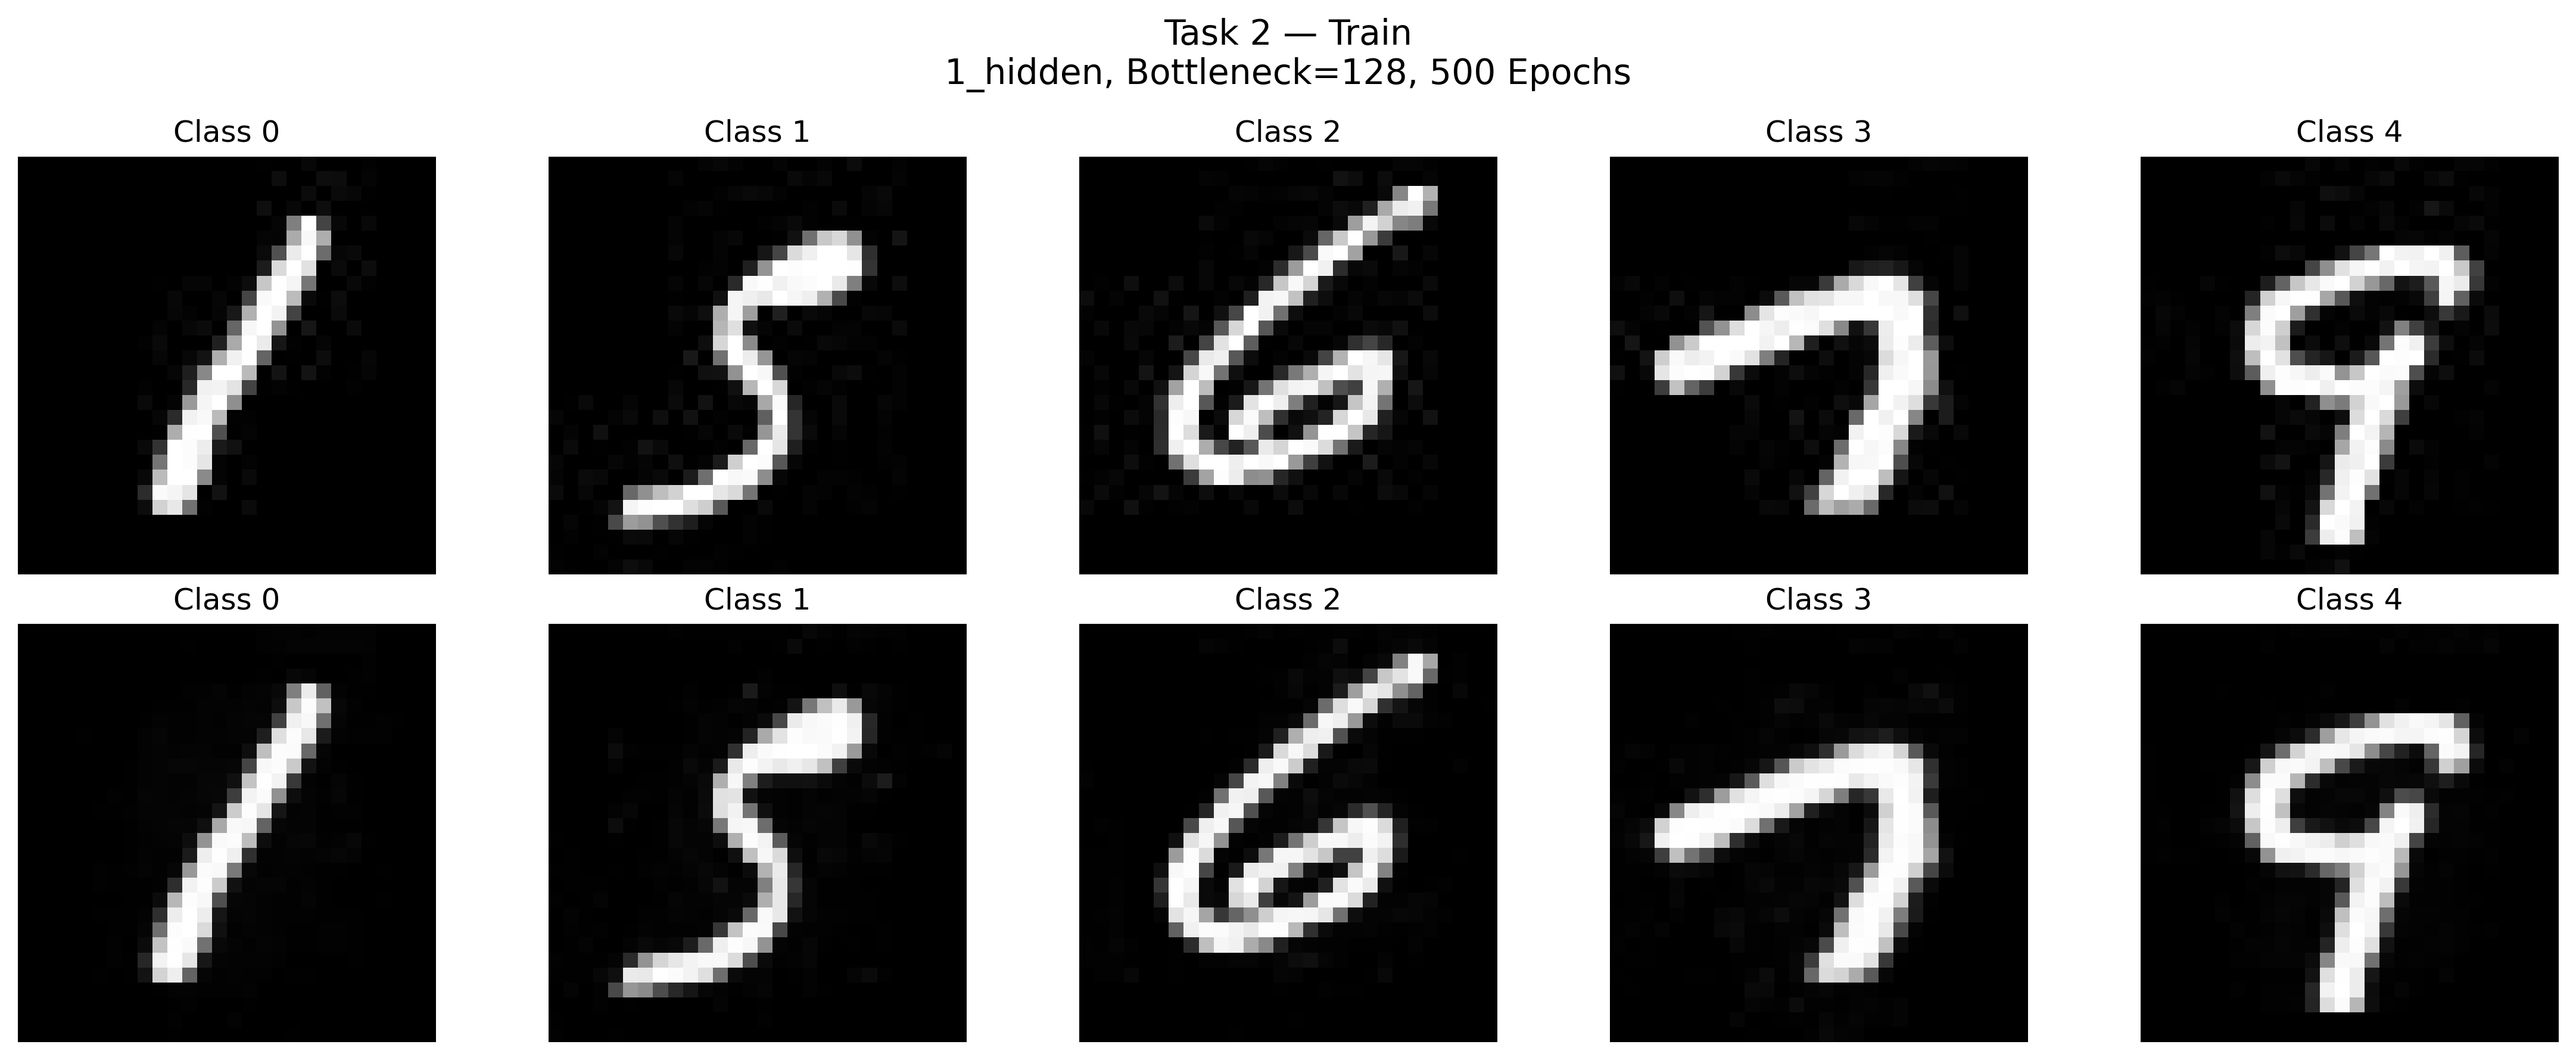
\includegraphics[width=0.96\linewidth,height=0.48\textheight,keepaspectratio]{figures/task2/model_reconstruction_visualization_500/train_1_hidden_bottleneck_128_500epochs.png}
\caption{Autoencoder reconstruction visualization: train 1 hidden with bottleneck of 128 neurons.}
\label{fig:task2_11}
\end{figure}

\begin{figure}[H]
\centering
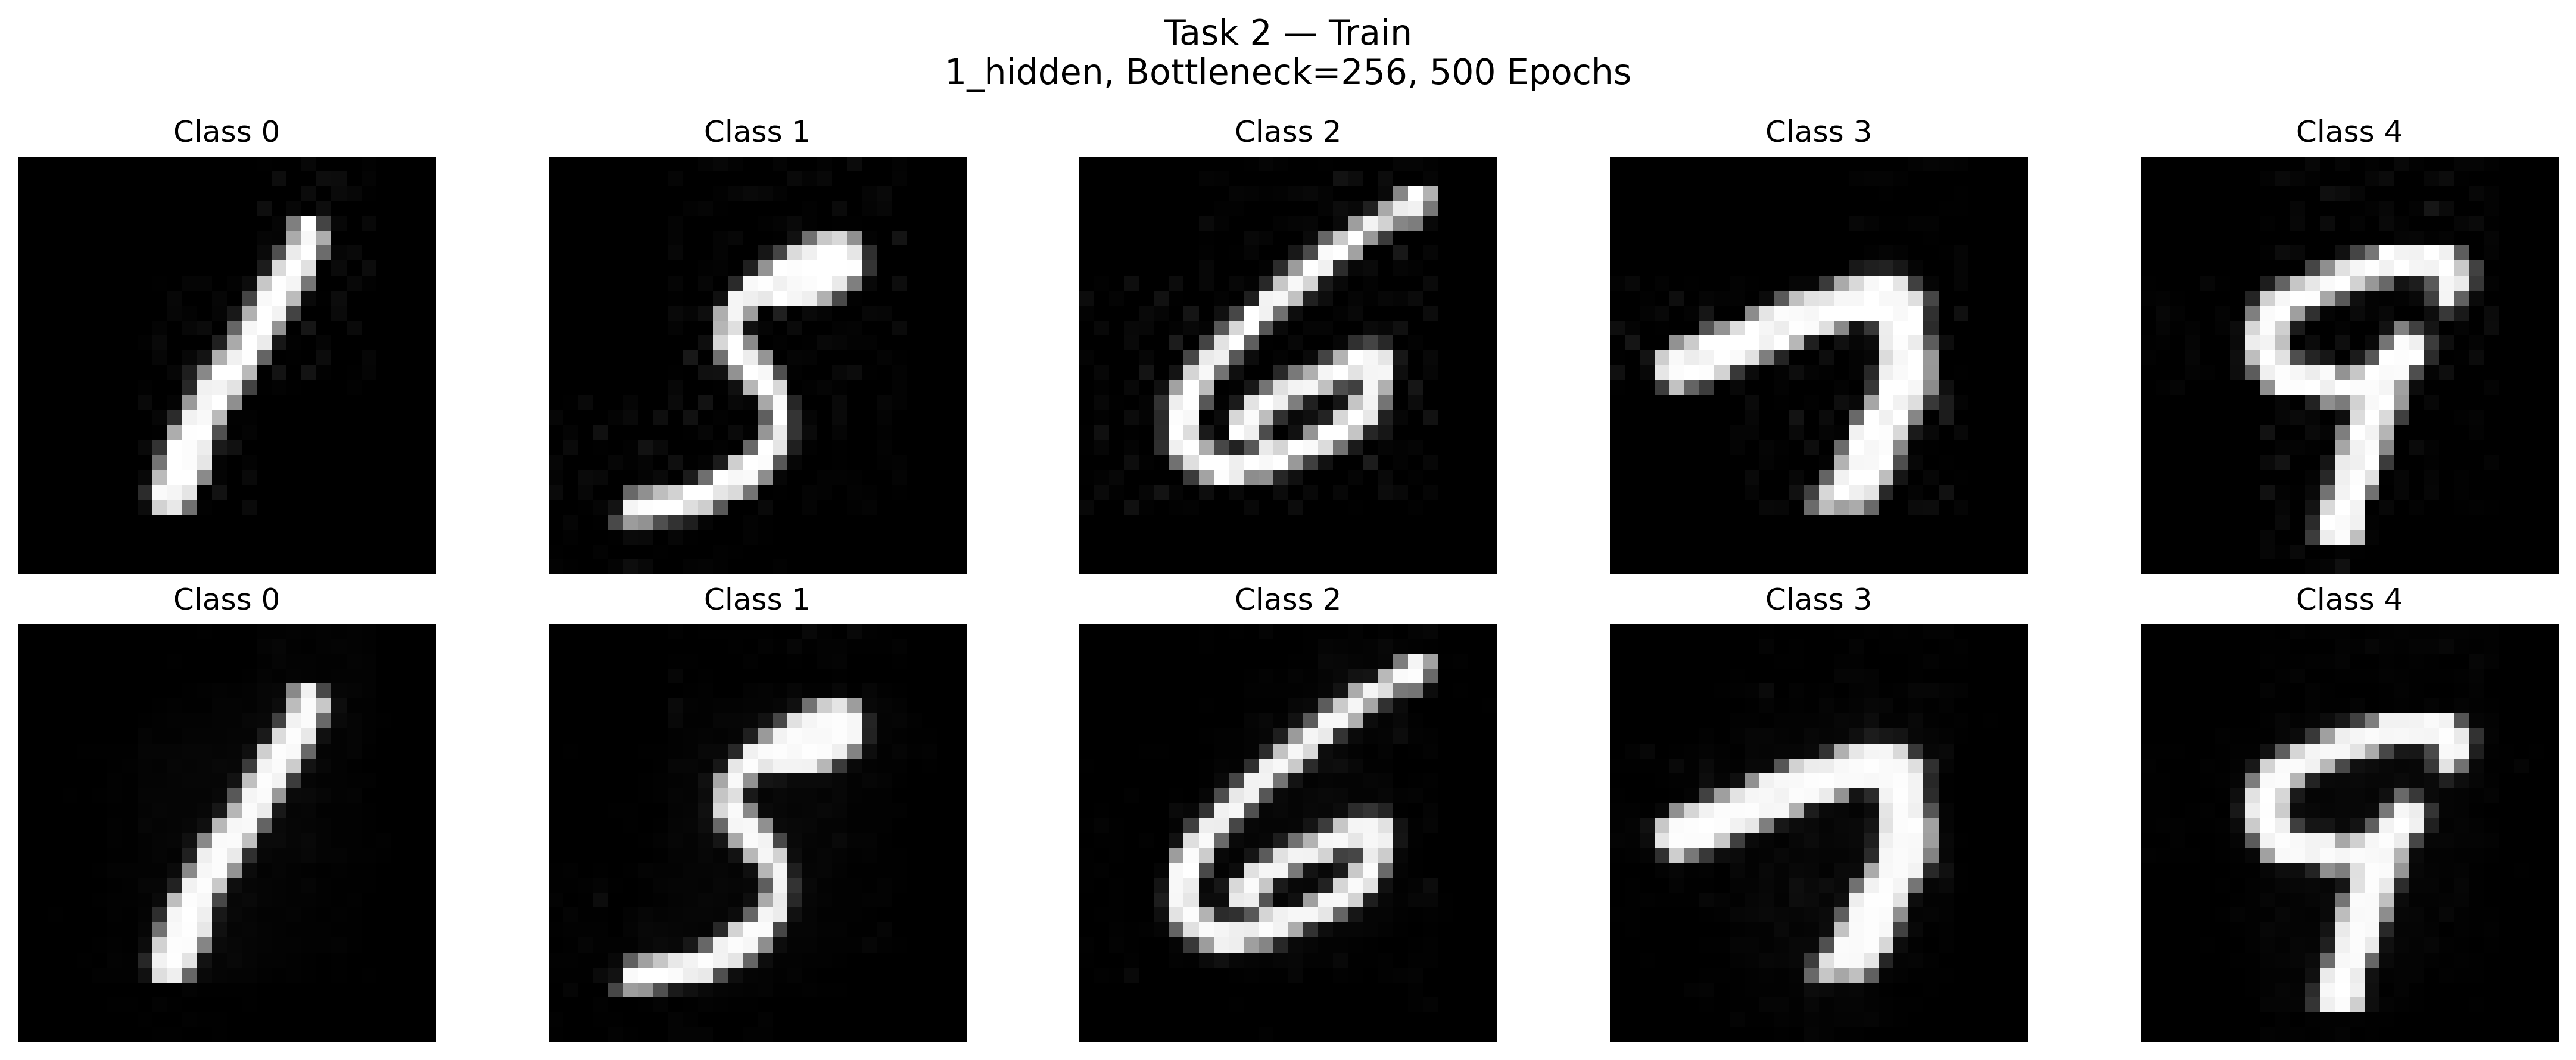
\includegraphics[width=0.96\linewidth,height=0.48\textheight,keepaspectratio]{figures/task2/model_reconstruction_visualization_500/train_1_hidden_bottleneck_256_500epochs.png}
\caption{Autoencoder reconstruction visualization: train 1 hidden with bottleneck of 256 neurons.}
\label{fig:task2_12}
\end{figure}

\begin{figure}[H]
\centering
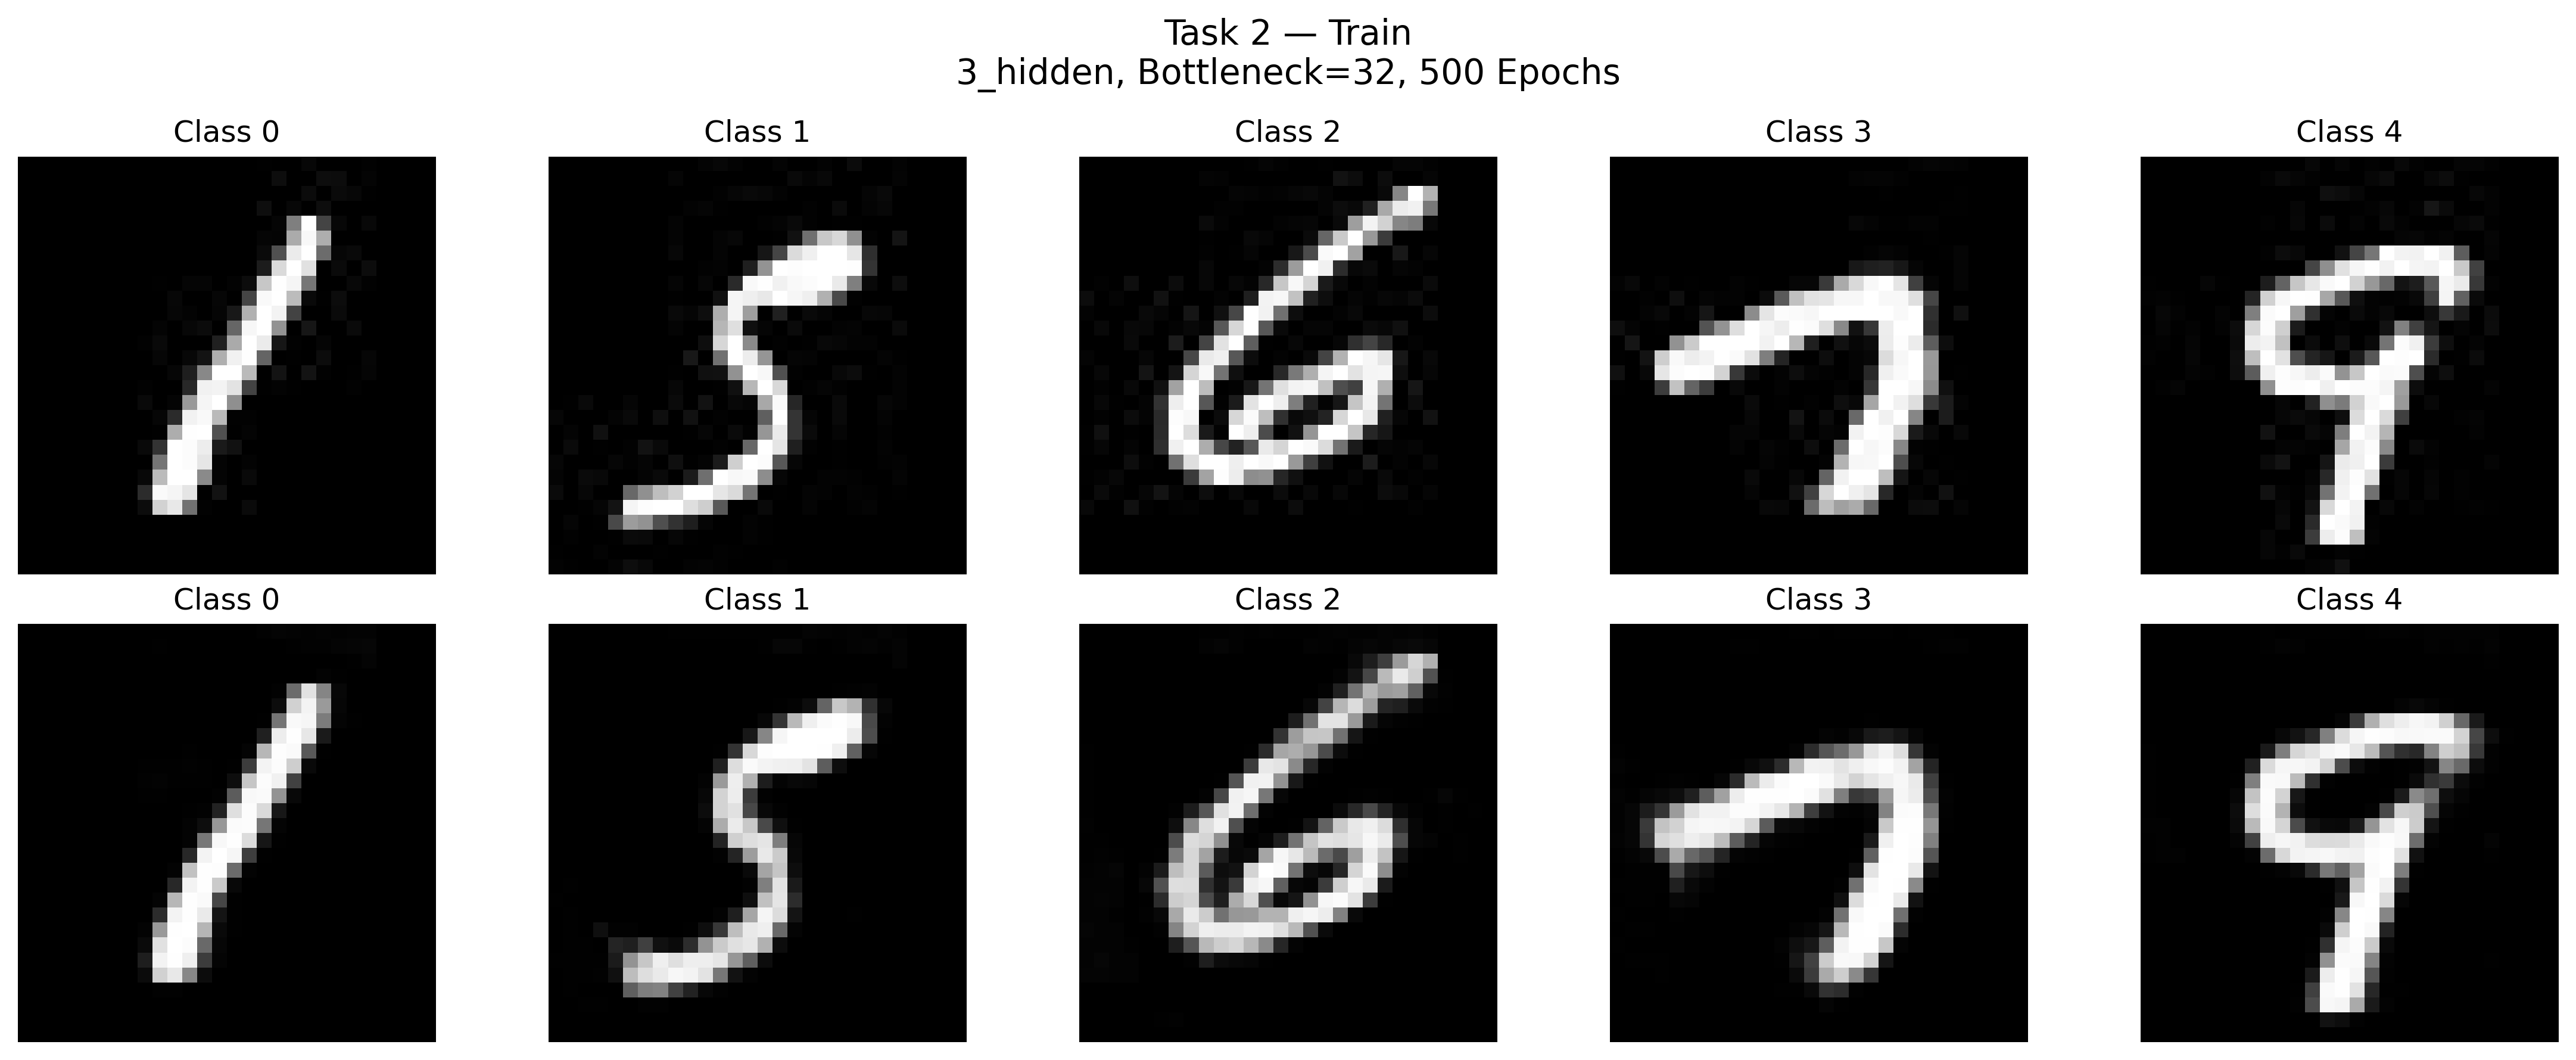
\includegraphics[width=0.96\linewidth,height=0.48\textheight,keepaspectratio]{figures/task2/model_reconstruction_visualization_500/train_3_hidden_bottleneck_32_500epochs.png}
\caption{Autoencoder reconstruction visualization: train 3 hidden with bottleneck of 32 neurons.}
\label{fig:task2_13}
\end{figure}

\begin{figure}[H]
\centering
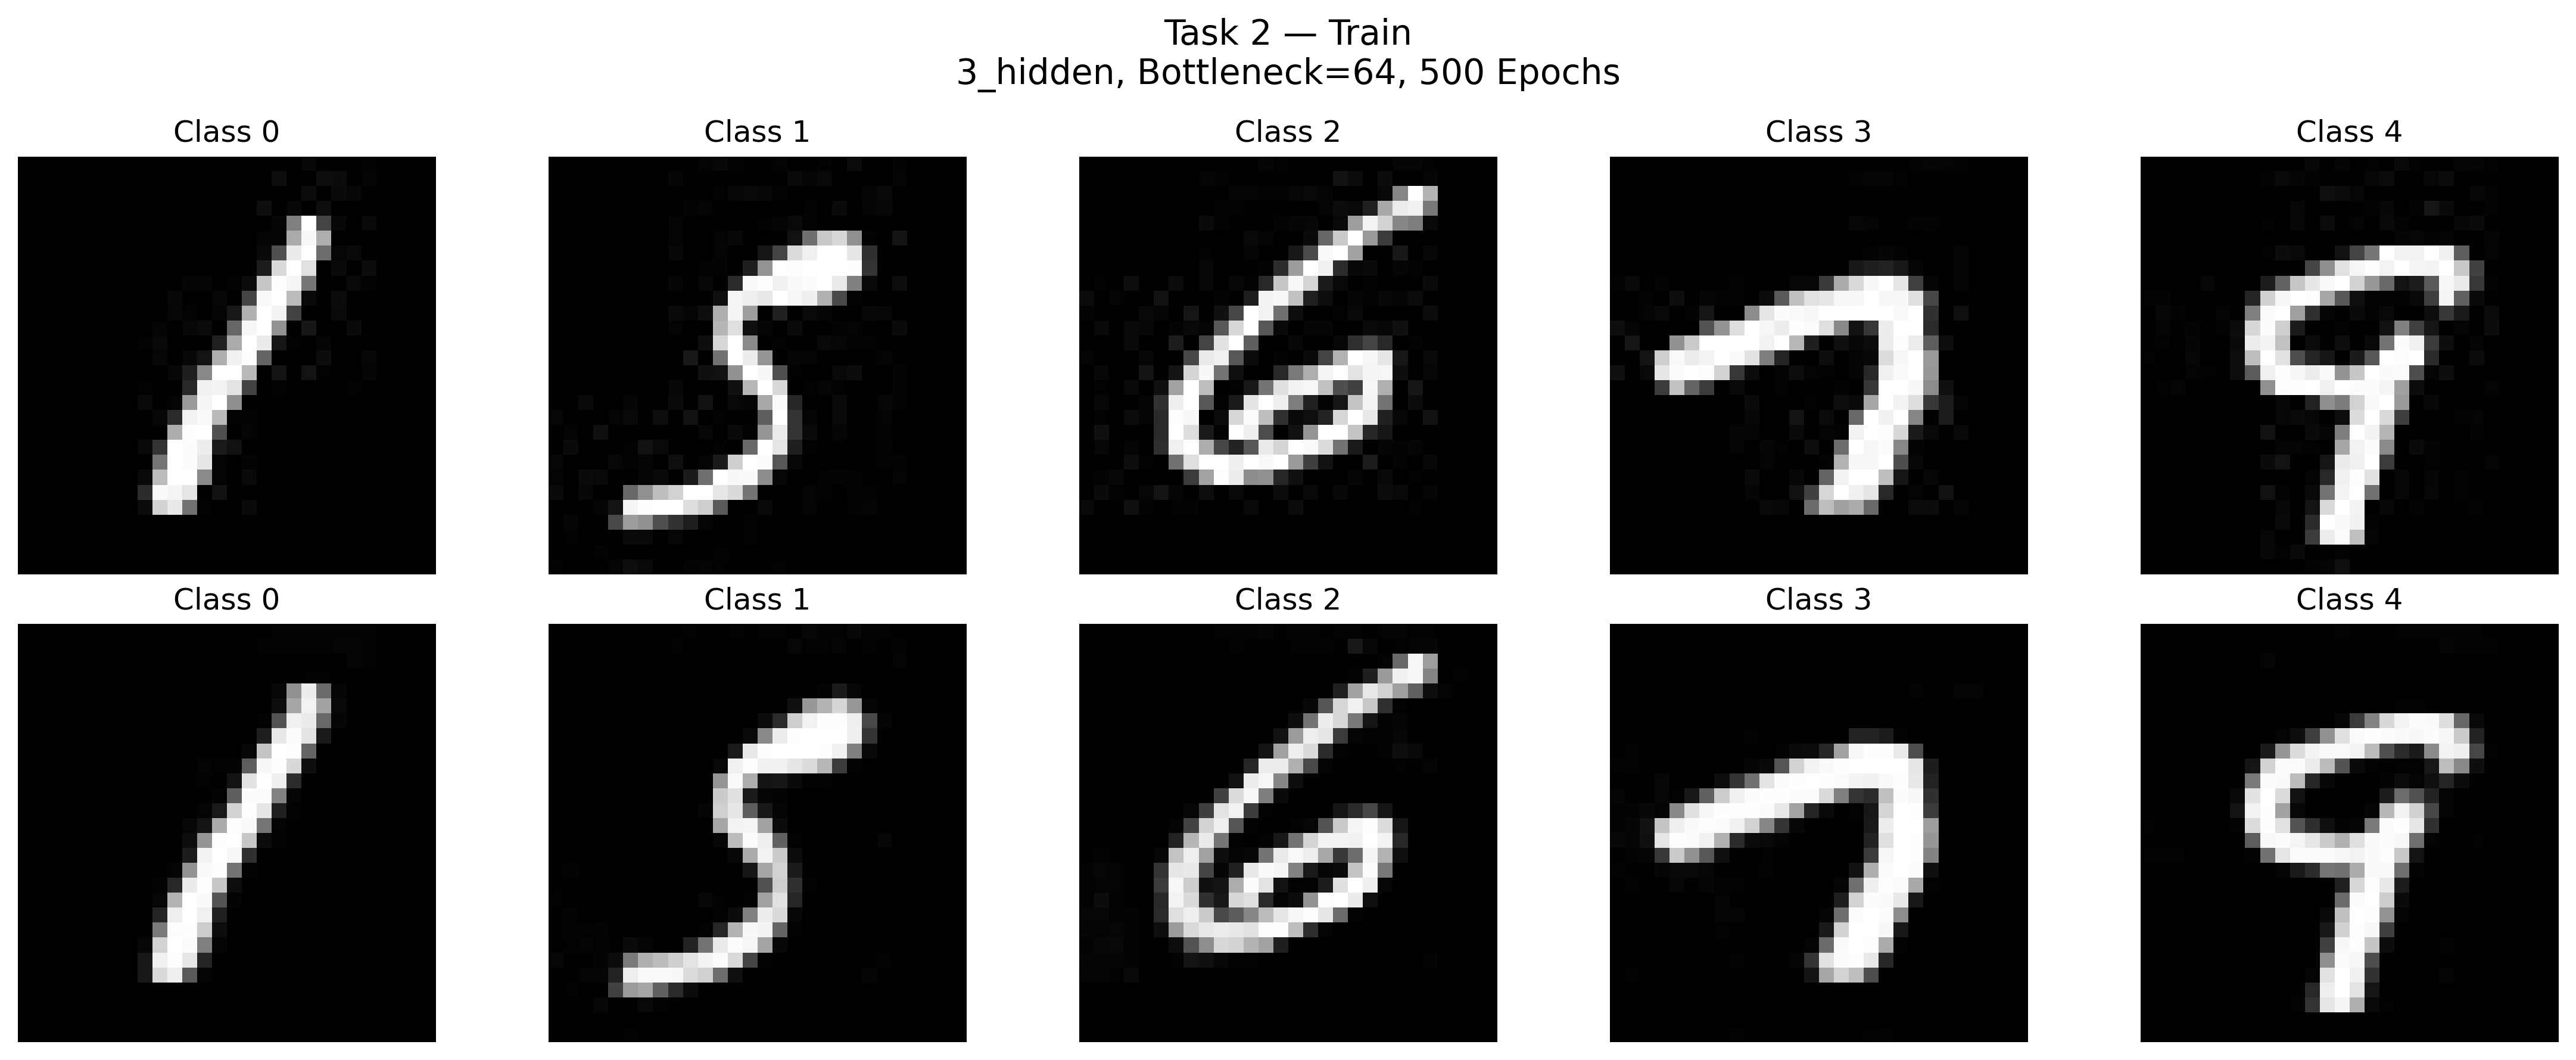
\includegraphics[width=0.96\linewidth,height=0.48\textheight,keepaspectratio]{figures/task2/model_reconstruction_visualization_500/train_3_hidden_bottleneck_64_500epochs.png}
\caption{Autoencoder reconstruction visualization: train 3 hidden with bottleneck of 64 neurons.}
\label{fig:task2_14}
\end{figure}

\begin{figure}[H]
\centering
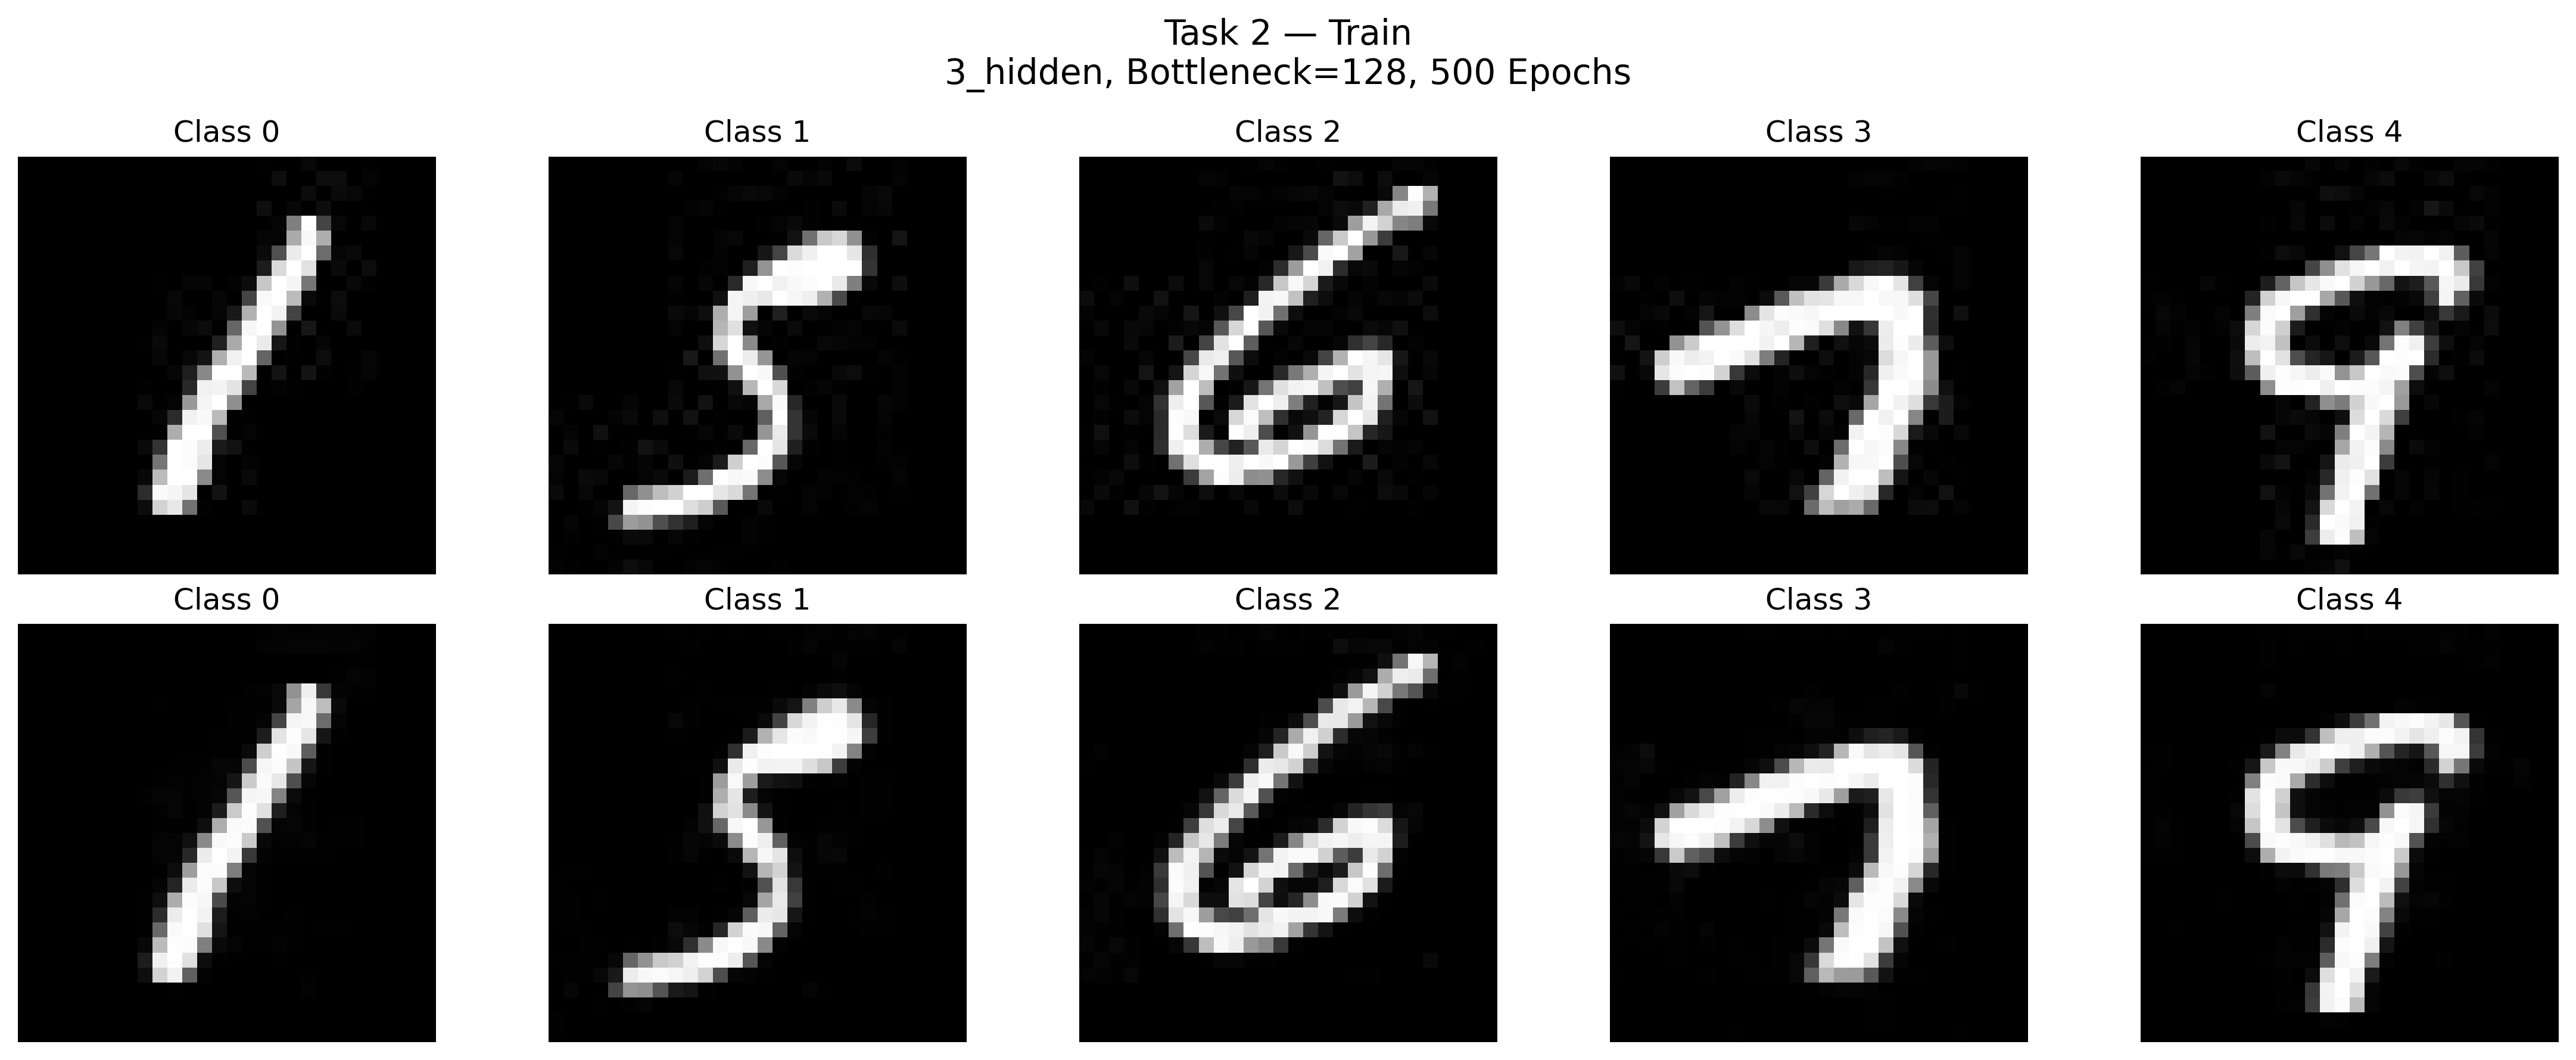
\includegraphics[width=0.96\linewidth,height=0.48\textheight,keepaspectratio]{figures/task2/model_reconstruction_visualization_500/train_3_hidden_bottleneck_128_500epochs.png}
\caption{Autoencoder reconstruction visualization: train 3 hidden with bottleneck of 128 neurons.}
\label{fig:task2_15}
\end{figure}

\begin{figure}[H]
\centering
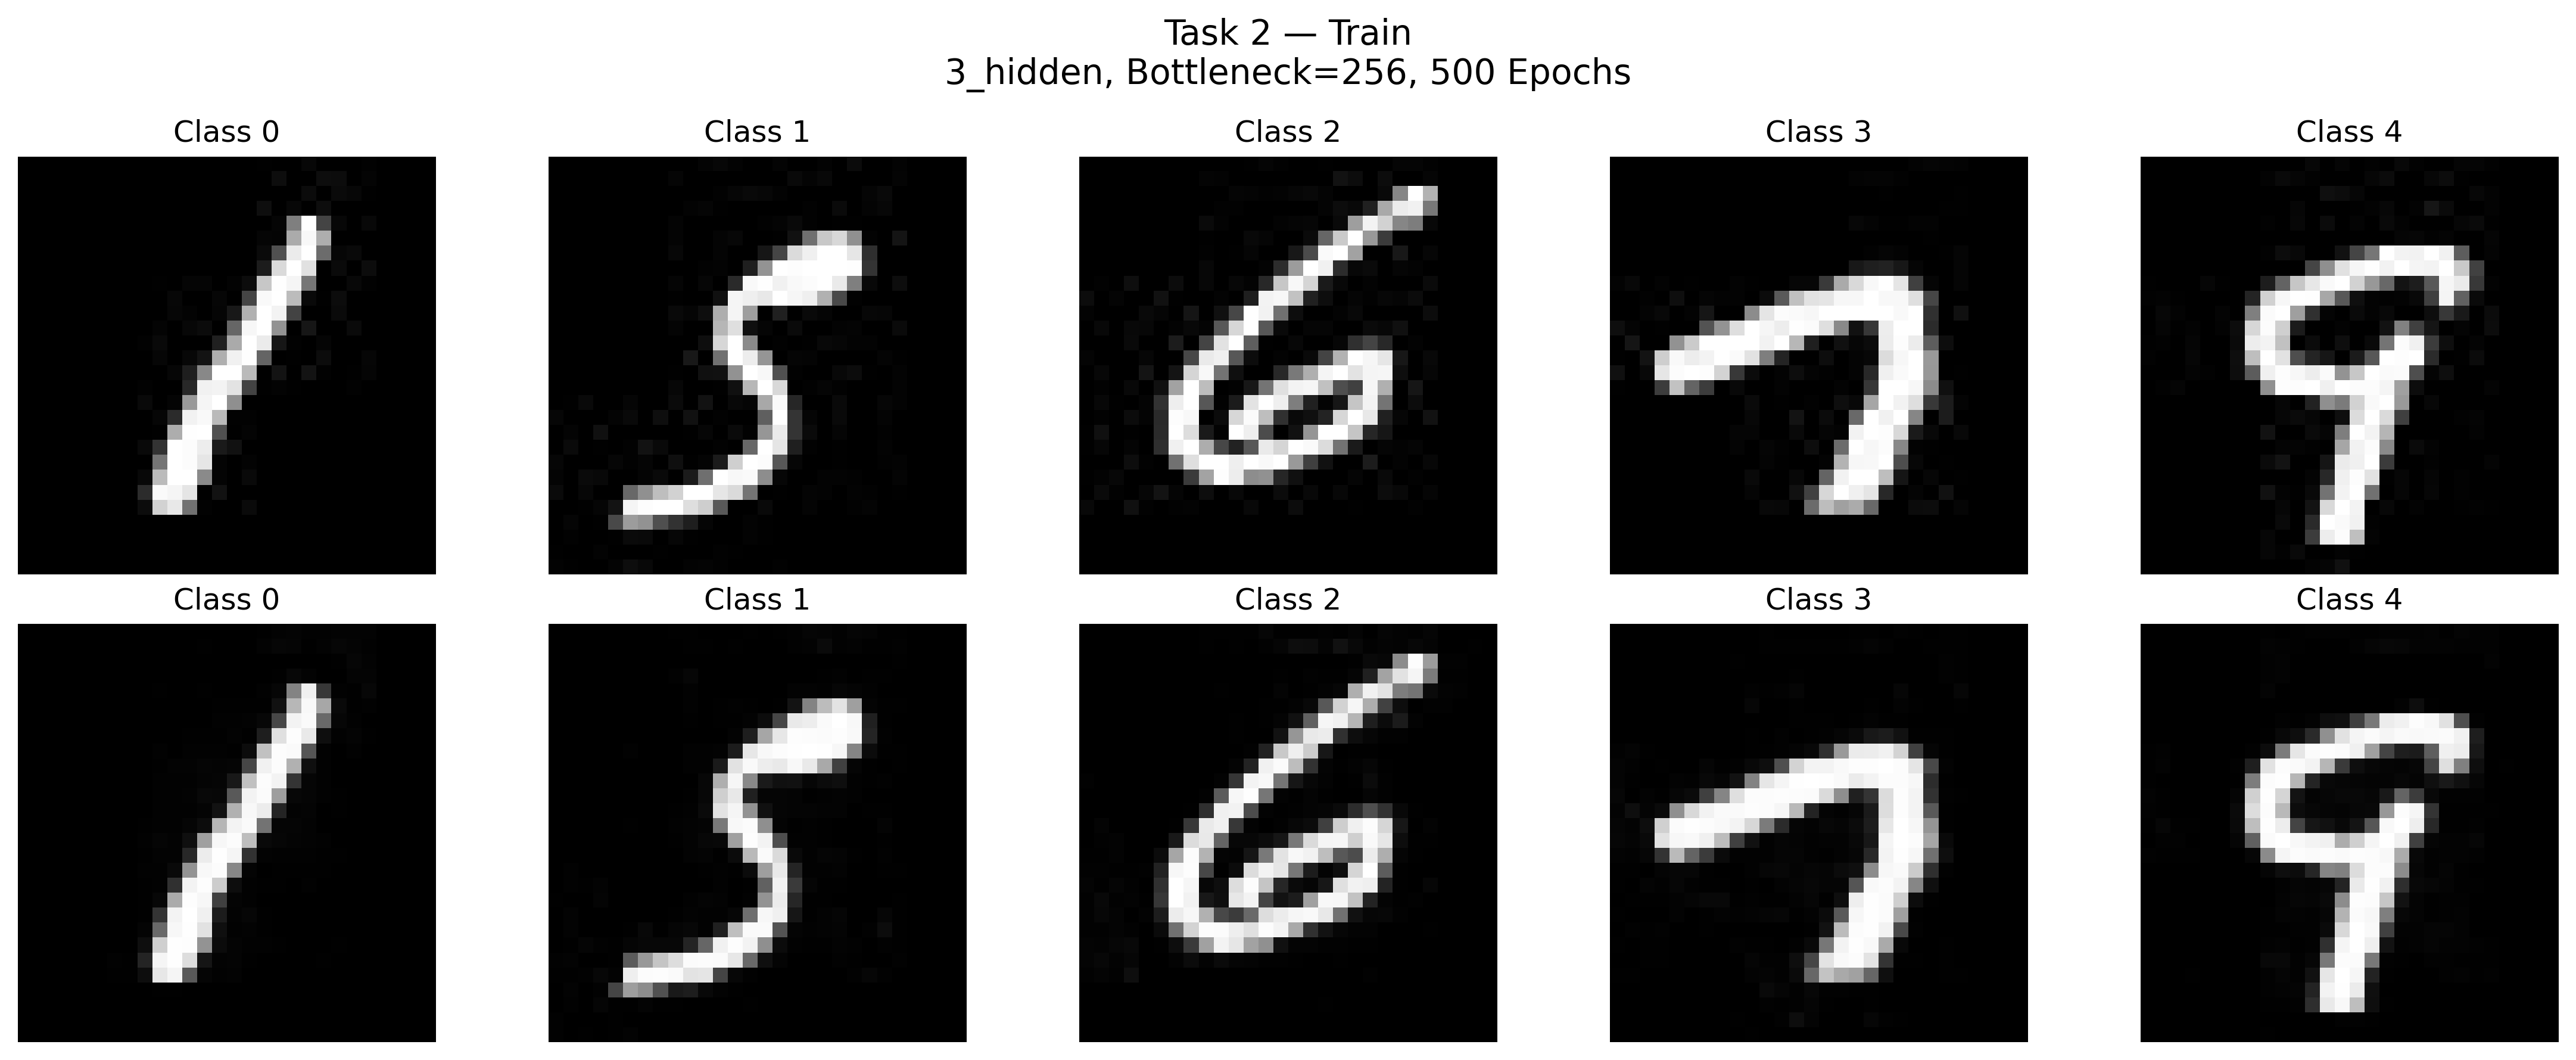
\includegraphics[width=0.96\linewidth,height=0.48\textheight,keepaspectratio]{figures/task2/model_reconstruction_visualization_500/train_3_hidden_bottleneck_256_500epochs.png}
\caption{Autoencoder reconstruction visualization: train 3 hidden with bottleneck of 256 neurons.}
\label{fig:task2_16}
\end{figure}

\begin{figure}[H]
\centering
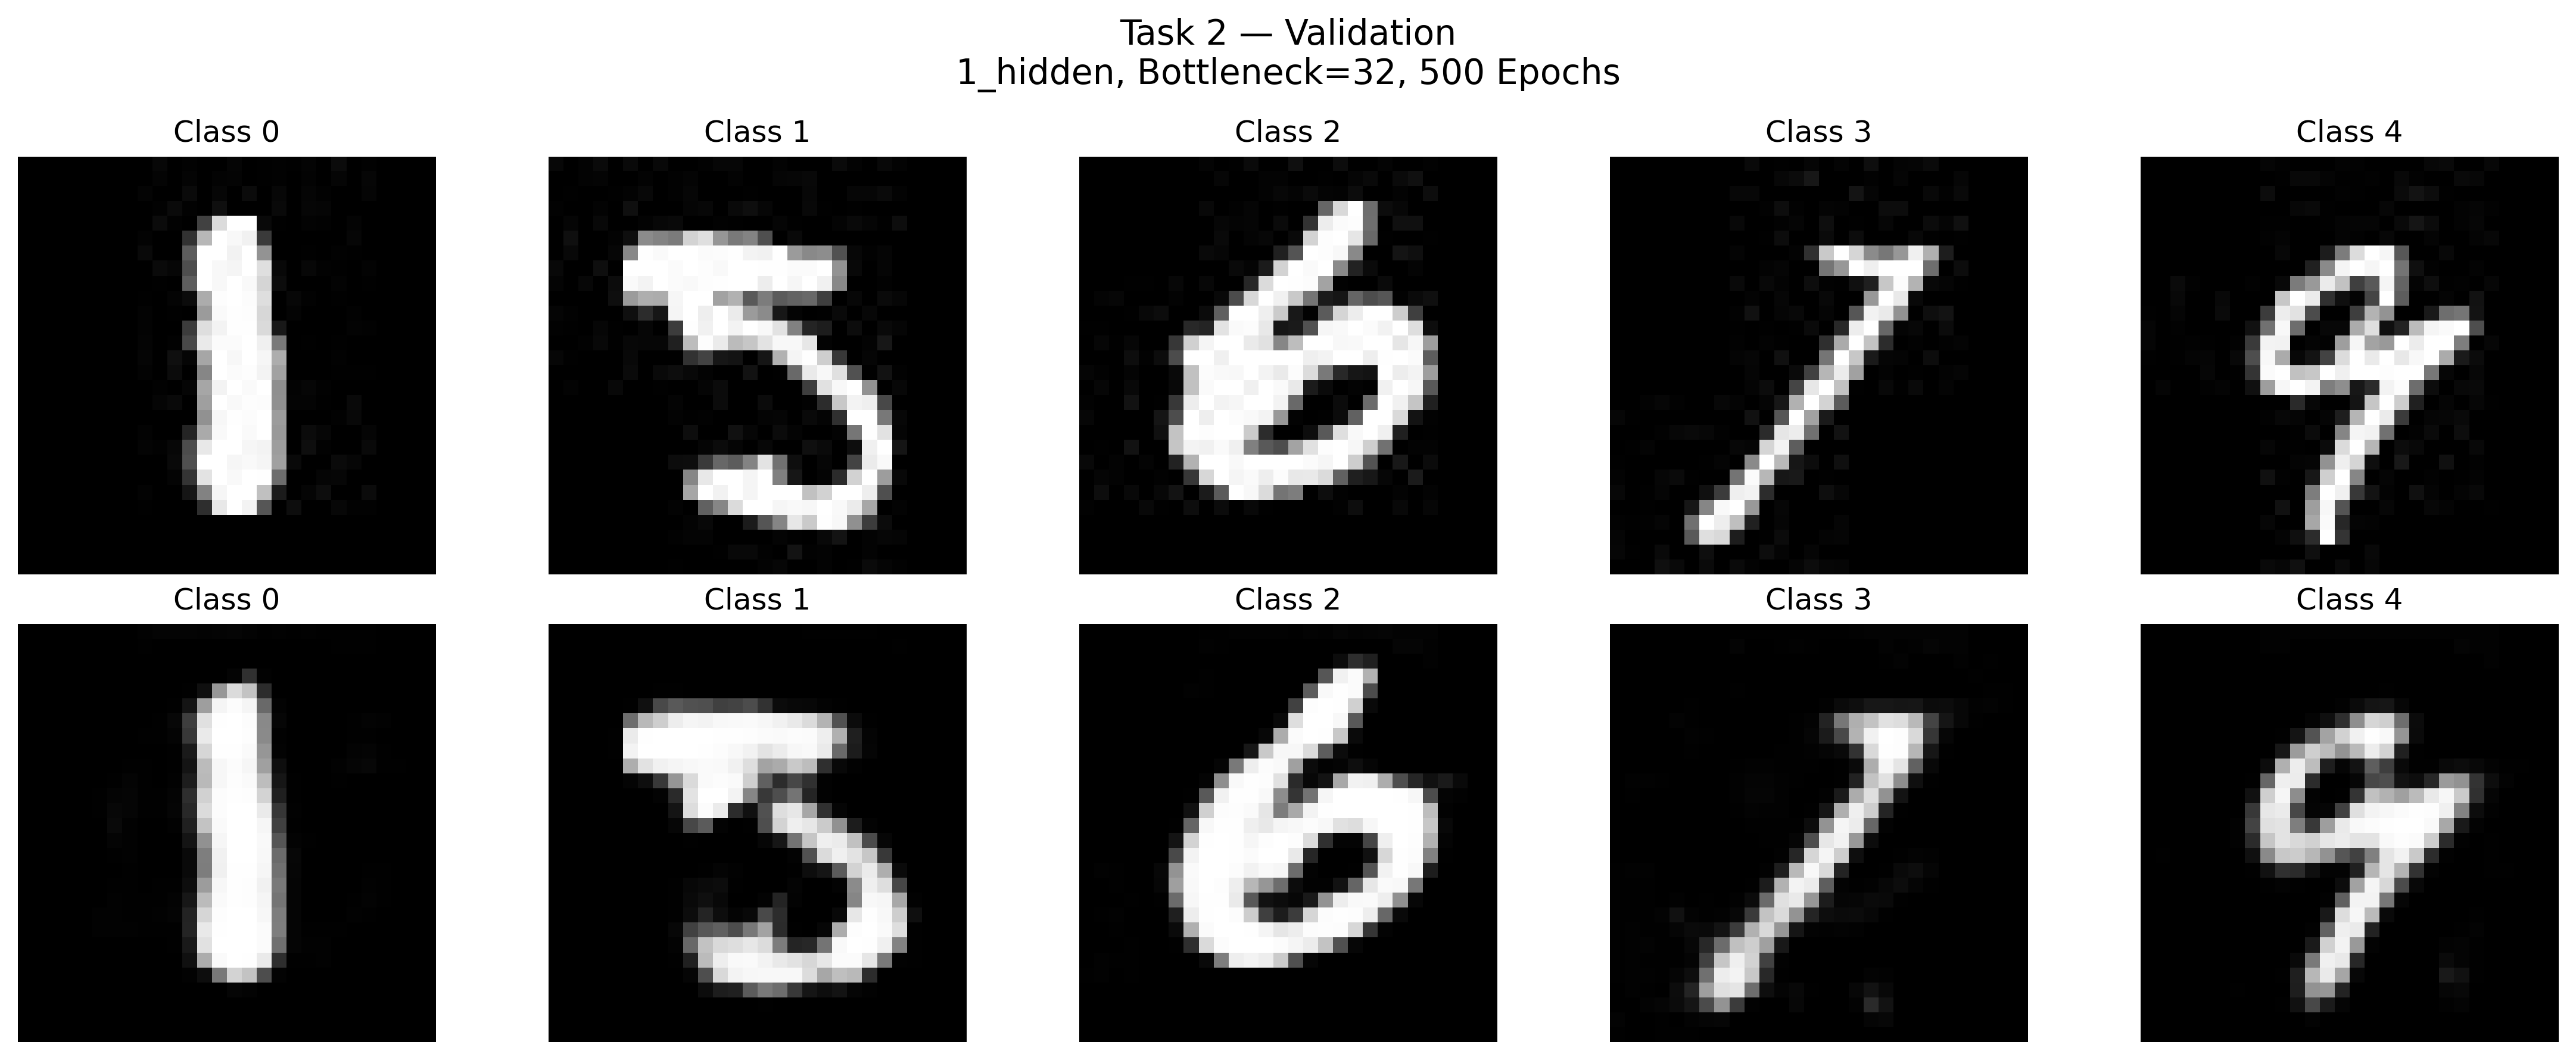
\includegraphics[width=0.96\linewidth,height=0.48\textheight,keepaspectratio]{figures/task2/model_reconstruction_visualization_500/validation_1_hidden_bottleneck_32_500epochs.png}
\caption{Autoencoder reconstruction visualization: validation 1 hidden with bottleneck of 32 neurons.}
\label{fig:task2_17}
\end{figure}

\begin{figure}[H]
\centering
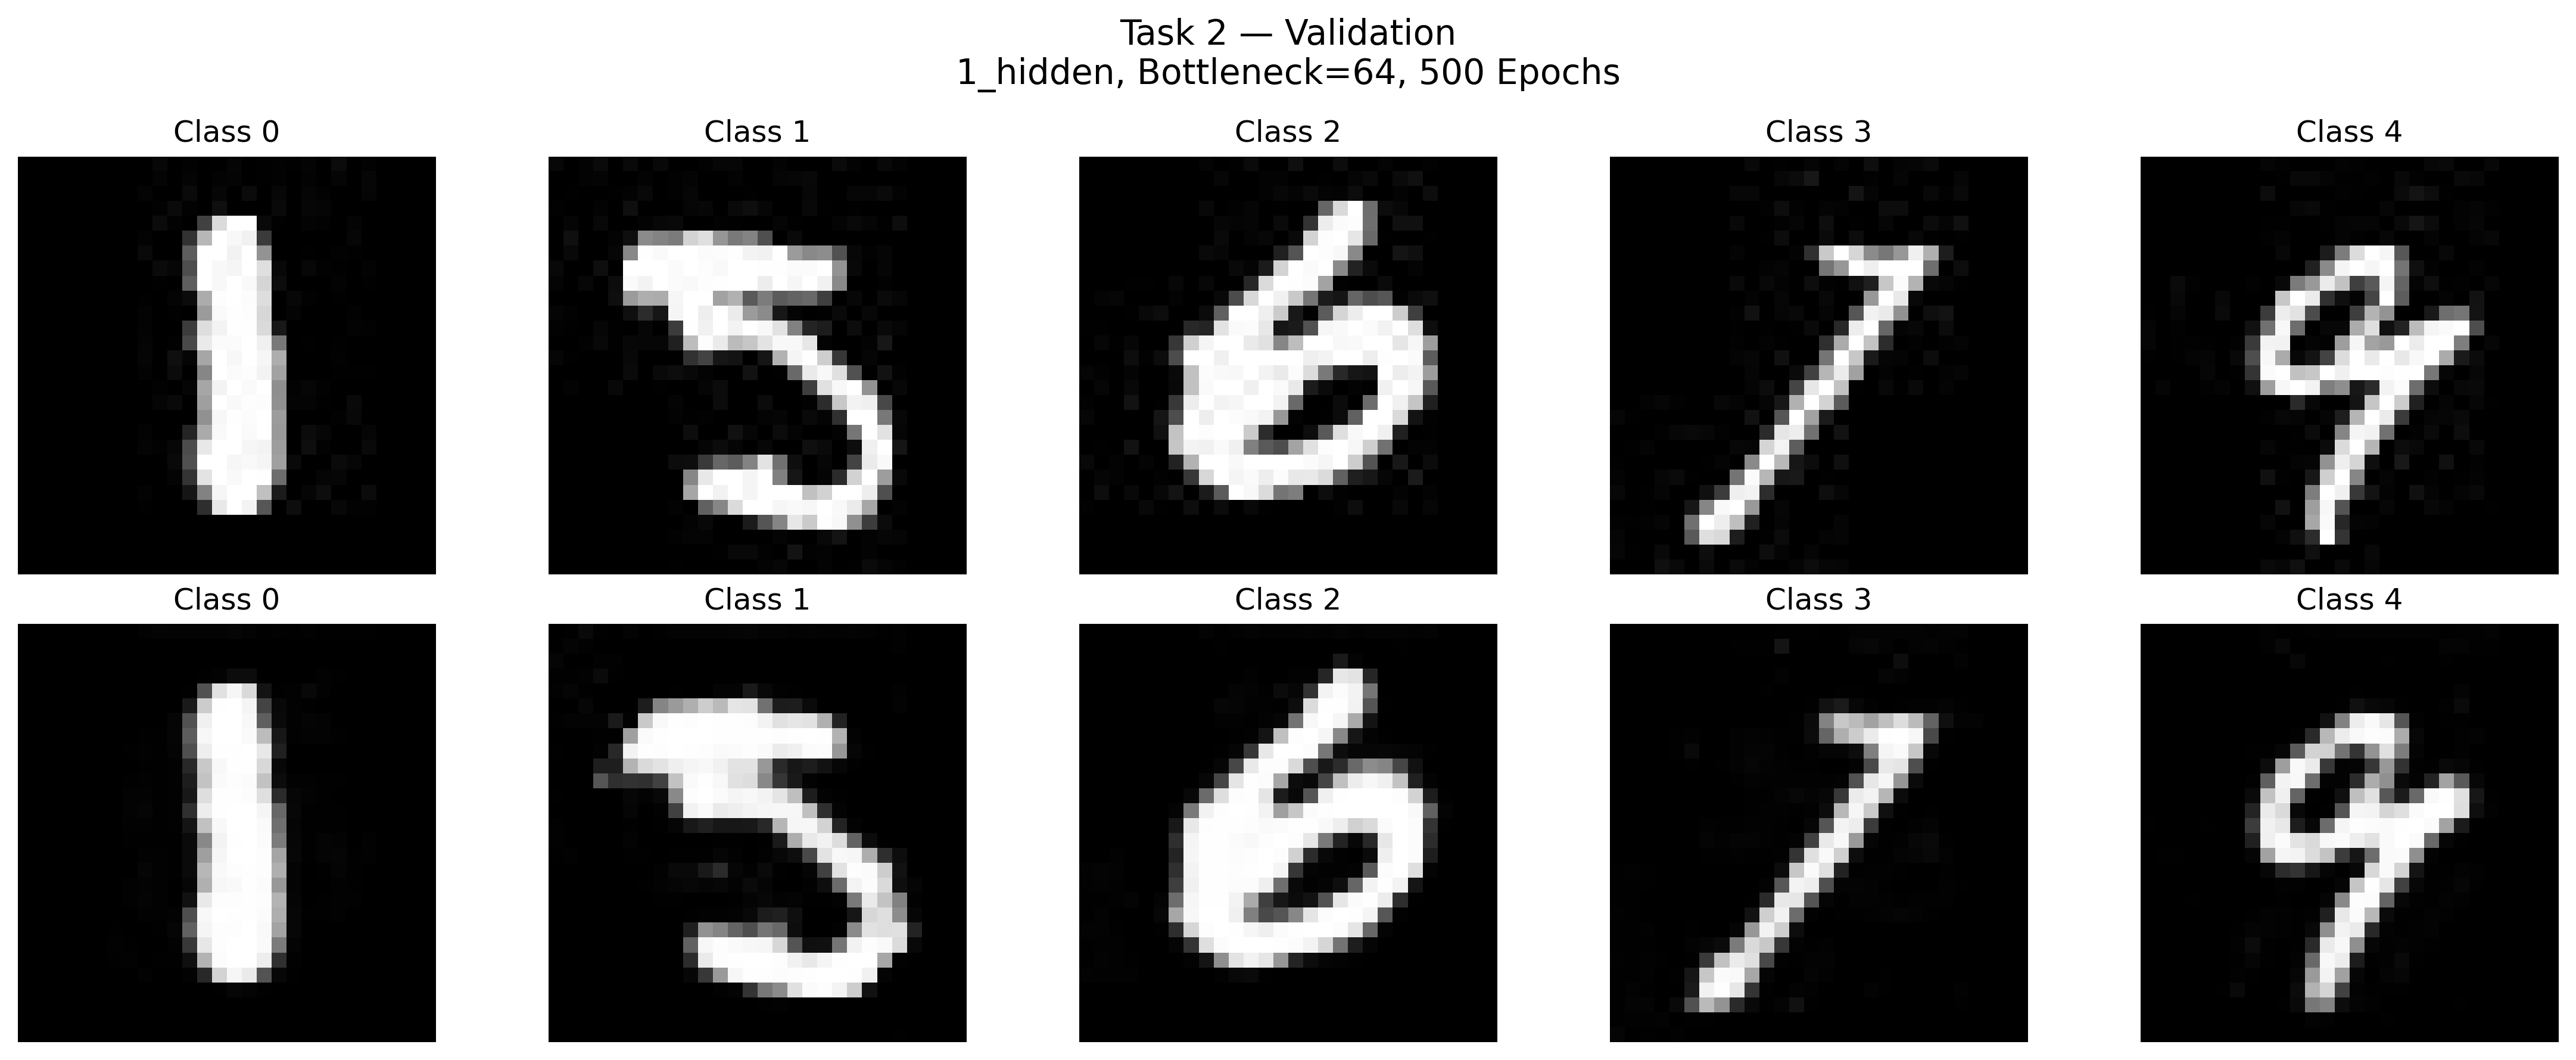
\includegraphics[width=0.96\linewidth,height=0.48\textheight,keepaspectratio]{figures/task2/model_reconstruction_visualization_500/validation_1_hidden_bottleneck_64_500epochs.png}
\caption{Autoencoder reconstruction visualization: validation 1 hidden with bottleneck of 64 neurons.}
\label{fig:task2_18}
\end{figure}

\begin{figure}[H]
\centering
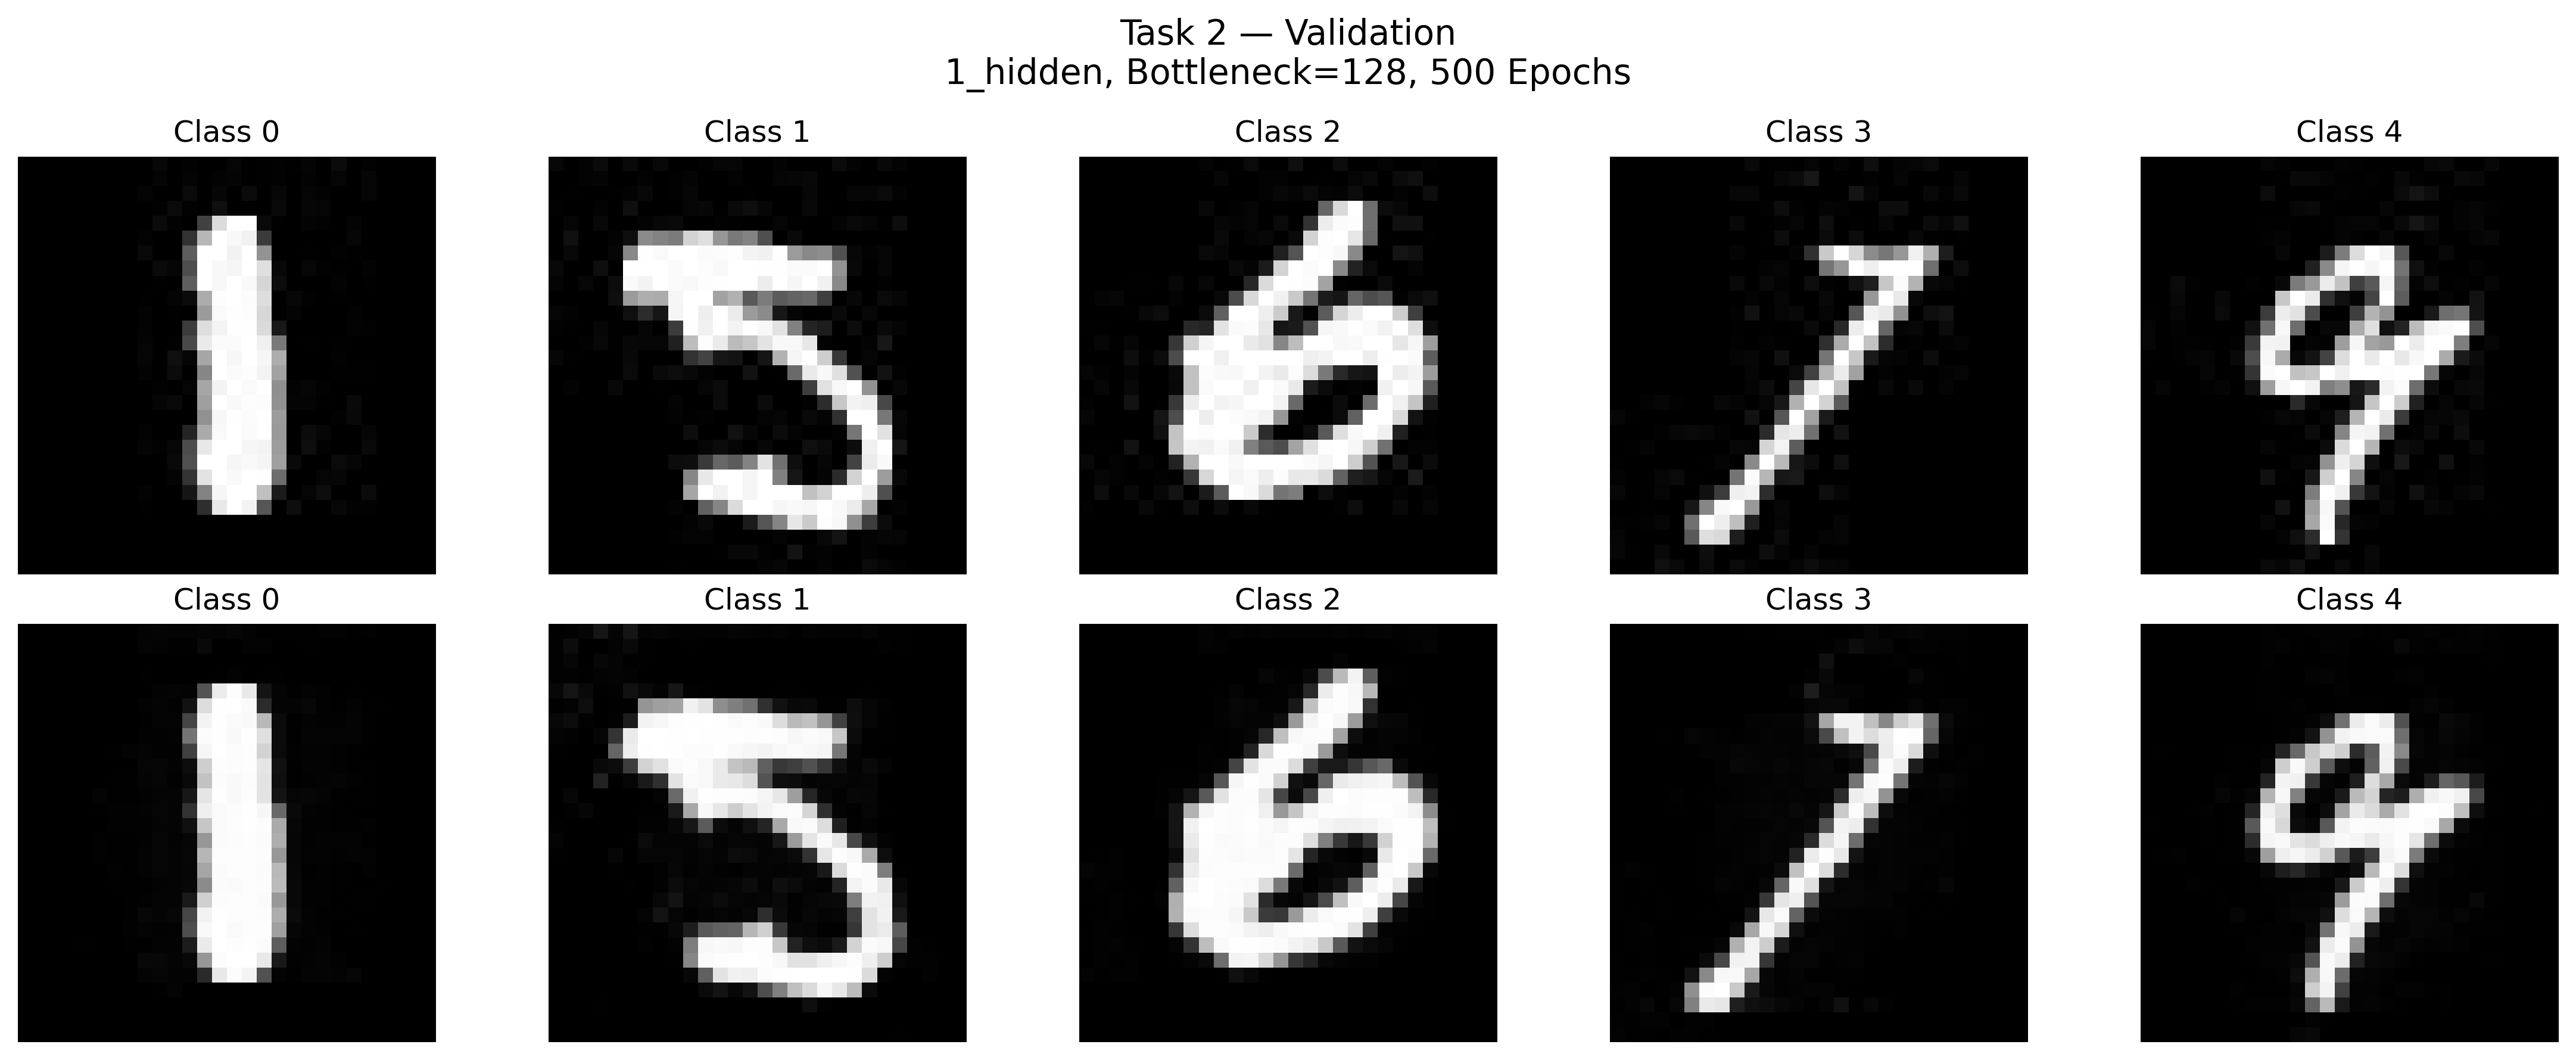
\includegraphics[width=0.96\linewidth,height=0.48\textheight,keepaspectratio]{figures/task2/model_reconstruction_visualization_500/validation_1_hidden_bottleneck_128_500epochs.png}
\caption{Autoencoder reconstruction visualization: validation 1 hidden with bottleneck of 128 neurons.}
\label{fig:task2_19}
\end{figure}

\begin{figure}[H]
\centering
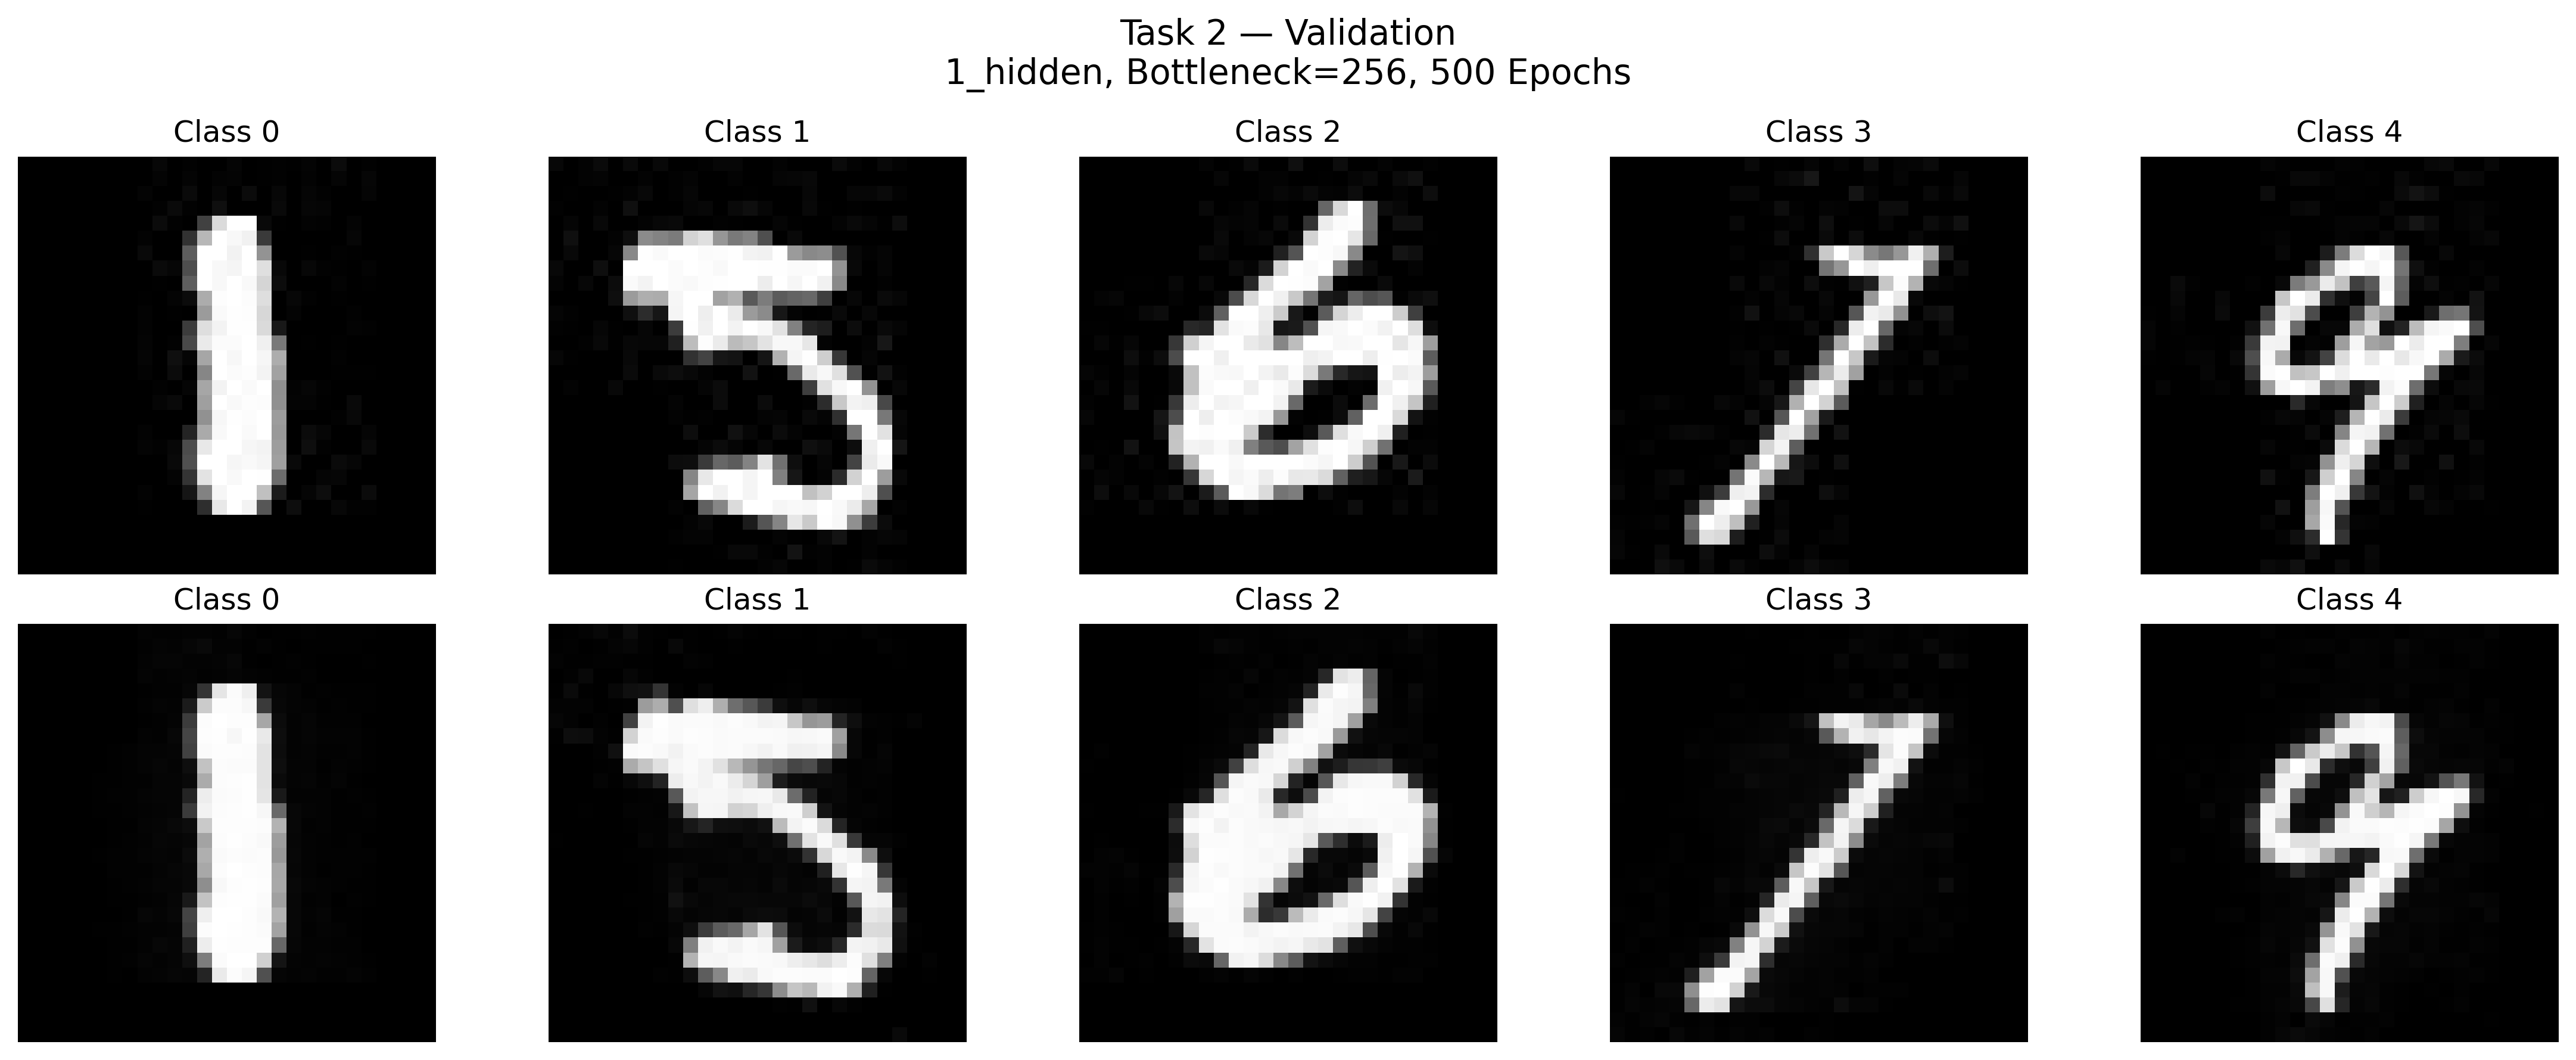
\includegraphics[width=0.96\linewidth,height=0.48\textheight,keepaspectratio]{figures/task2/model_reconstruction_visualization_500/validation_1_hidden_bottleneck_256_500epochs.png}
\caption{Autoencoder reconstruction visualization: validation 1 hidden with bottleneck of 256 neurons.}
\label{fig:task2_20}
\end{figure}

\begin{figure}[H]
\centering
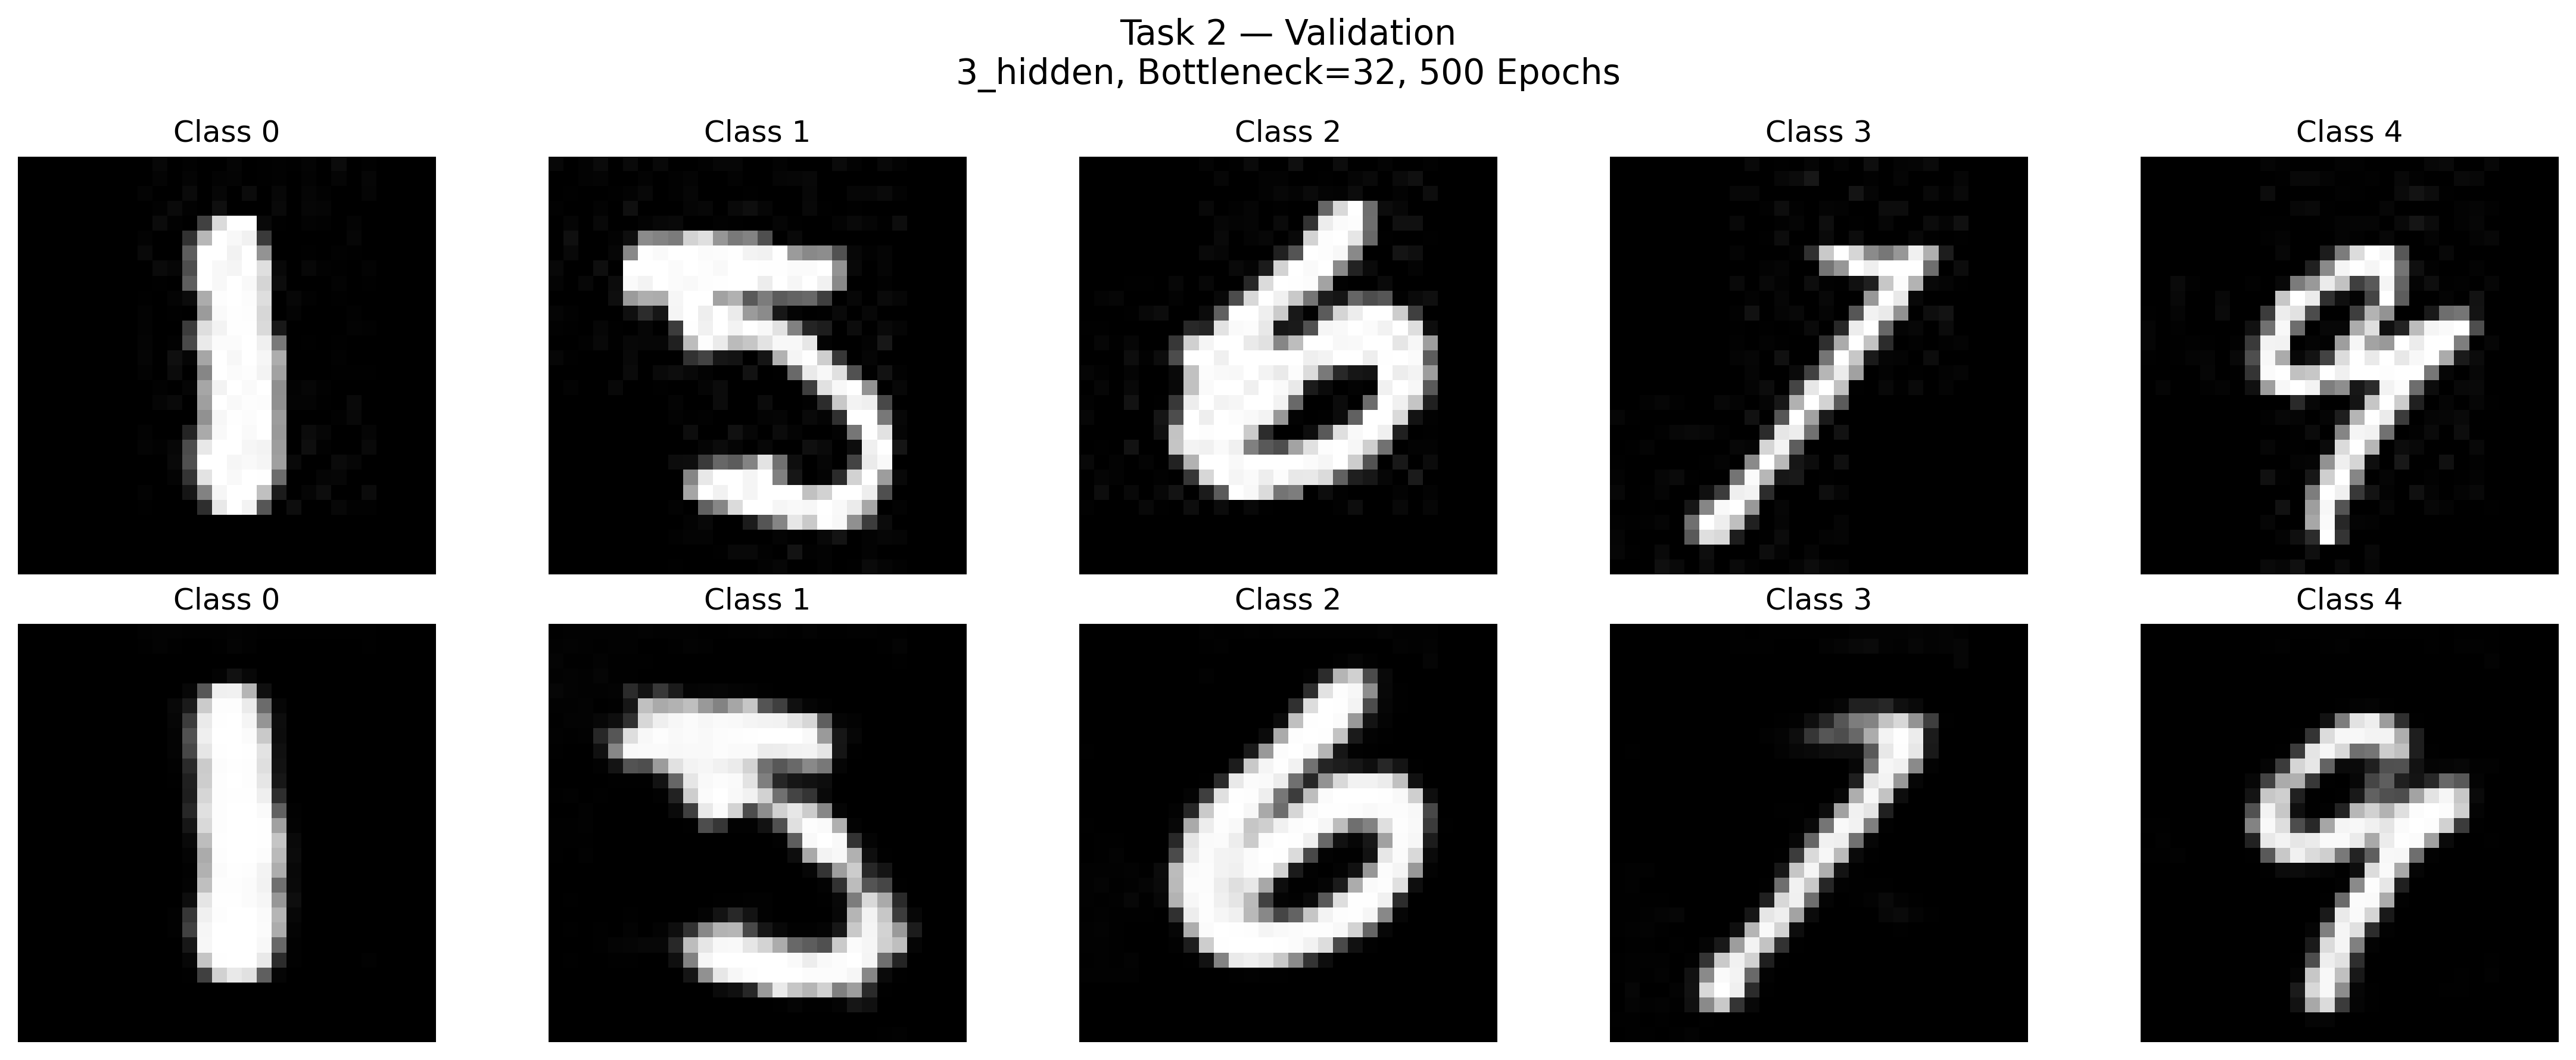
\includegraphics[width=0.96\linewidth,height=0.48\textheight,keepaspectratio]{figures/task2/model_reconstruction_visualization_500/validation_3_hidden_bottleneck_32_500epochs.png}
\caption{Autoencoder reconstruction visualization: validation 3 hidden with bottleneck of 32 neurons.}
\label{fig:task2_21}
\end{figure}

\begin{figure}[H]
\centering
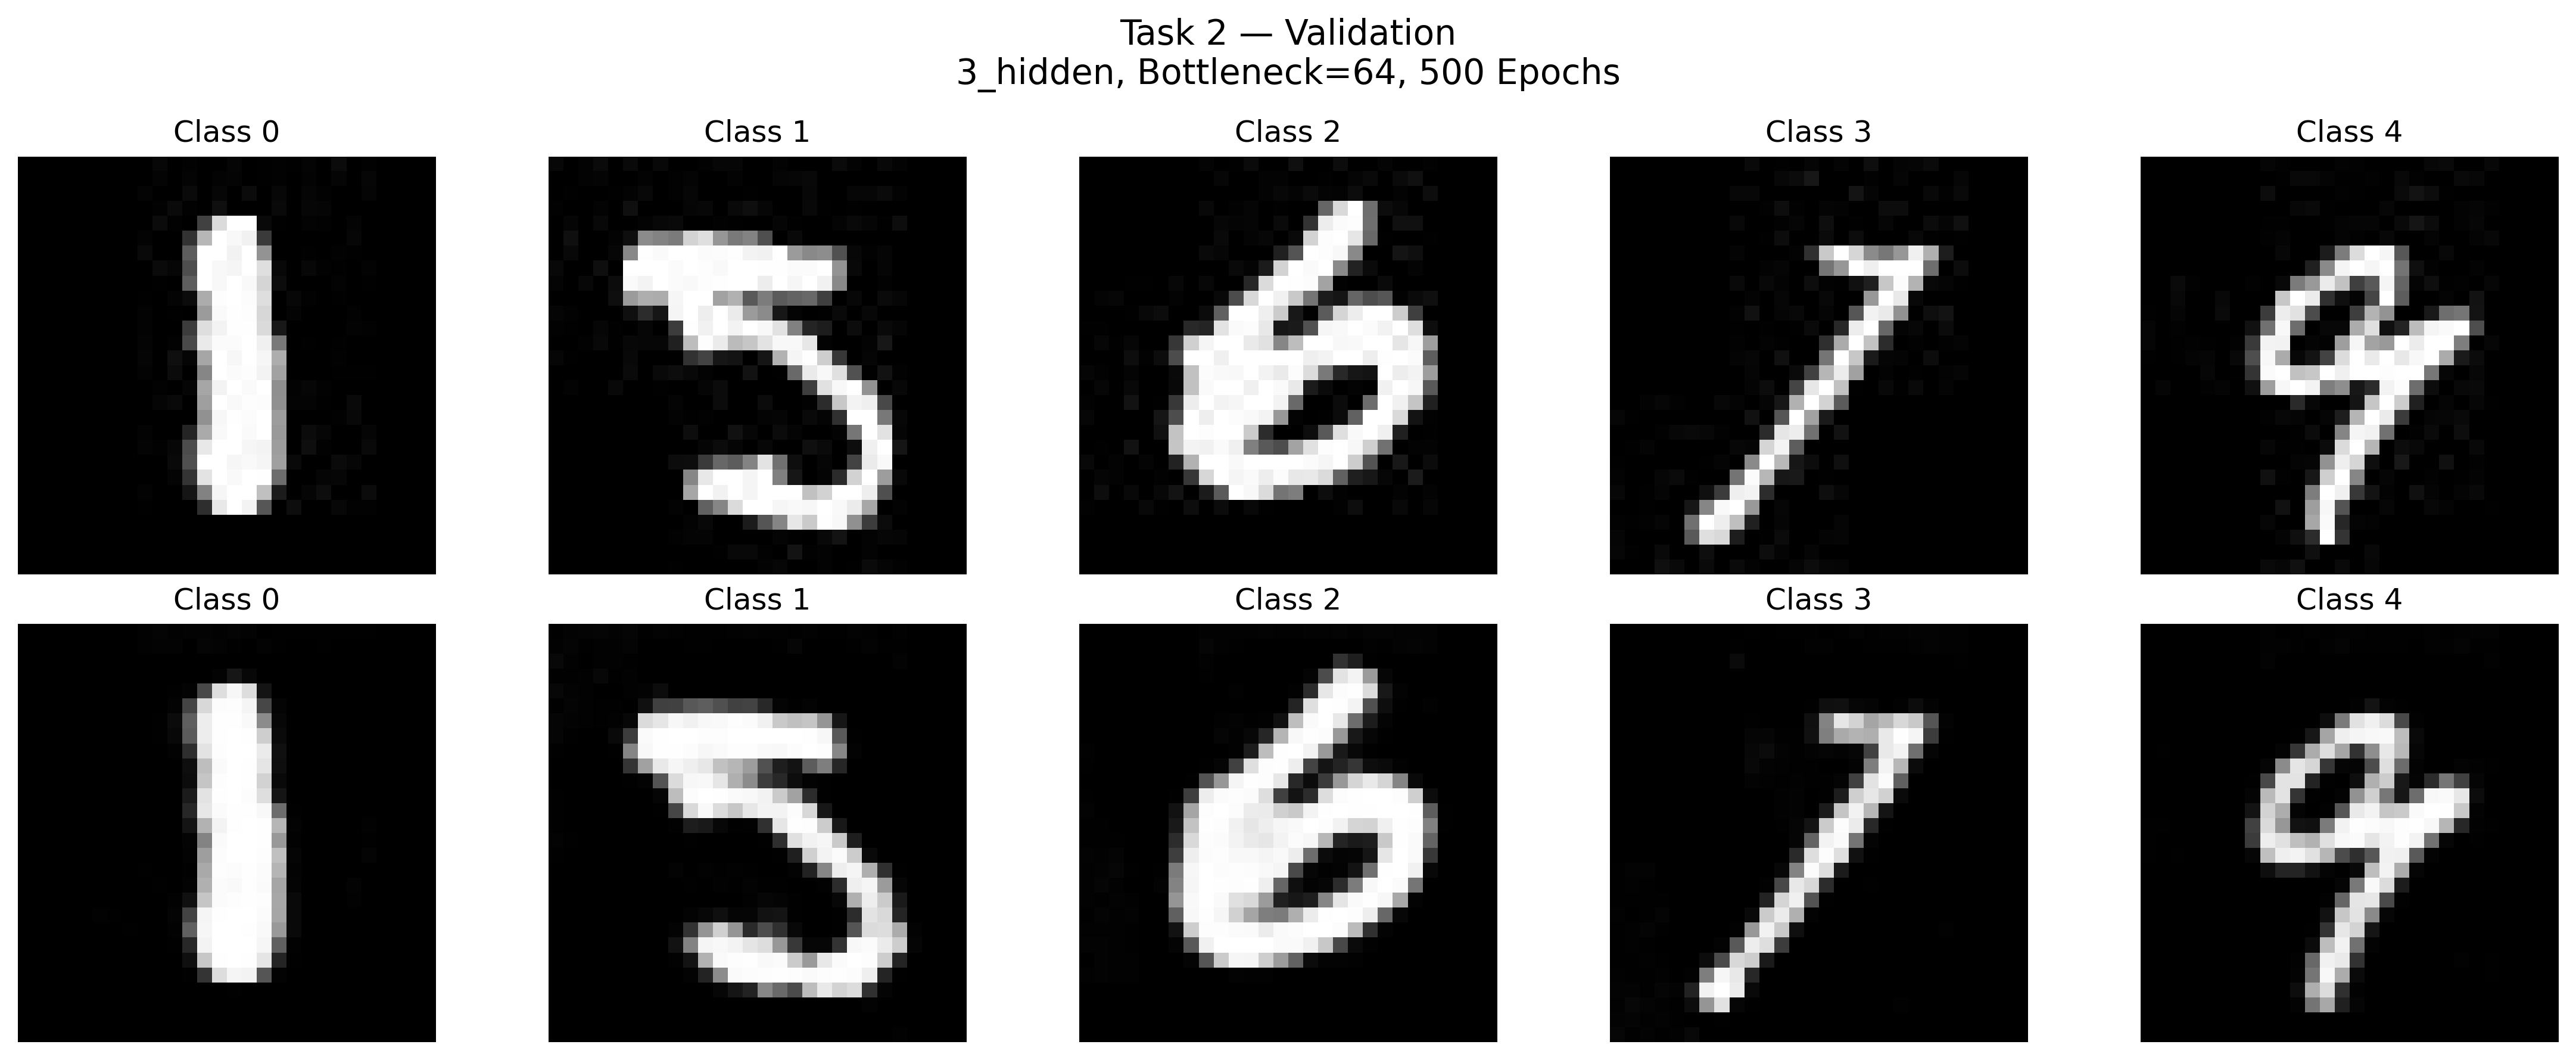
\includegraphics[width=0.96\linewidth,height=0.48\textheight,keepaspectratio]{figures/task2/model_reconstruction_visualization_500/validation_3_hidden_bottleneck_64_500epochs.png}
\caption{Autoencoder reconstruction visualization: validation 3 hidden with bottleneck of 64 neurons.}
\label{fig:task2_22}
\end{figure}

\begin{figure}[H]
\centering
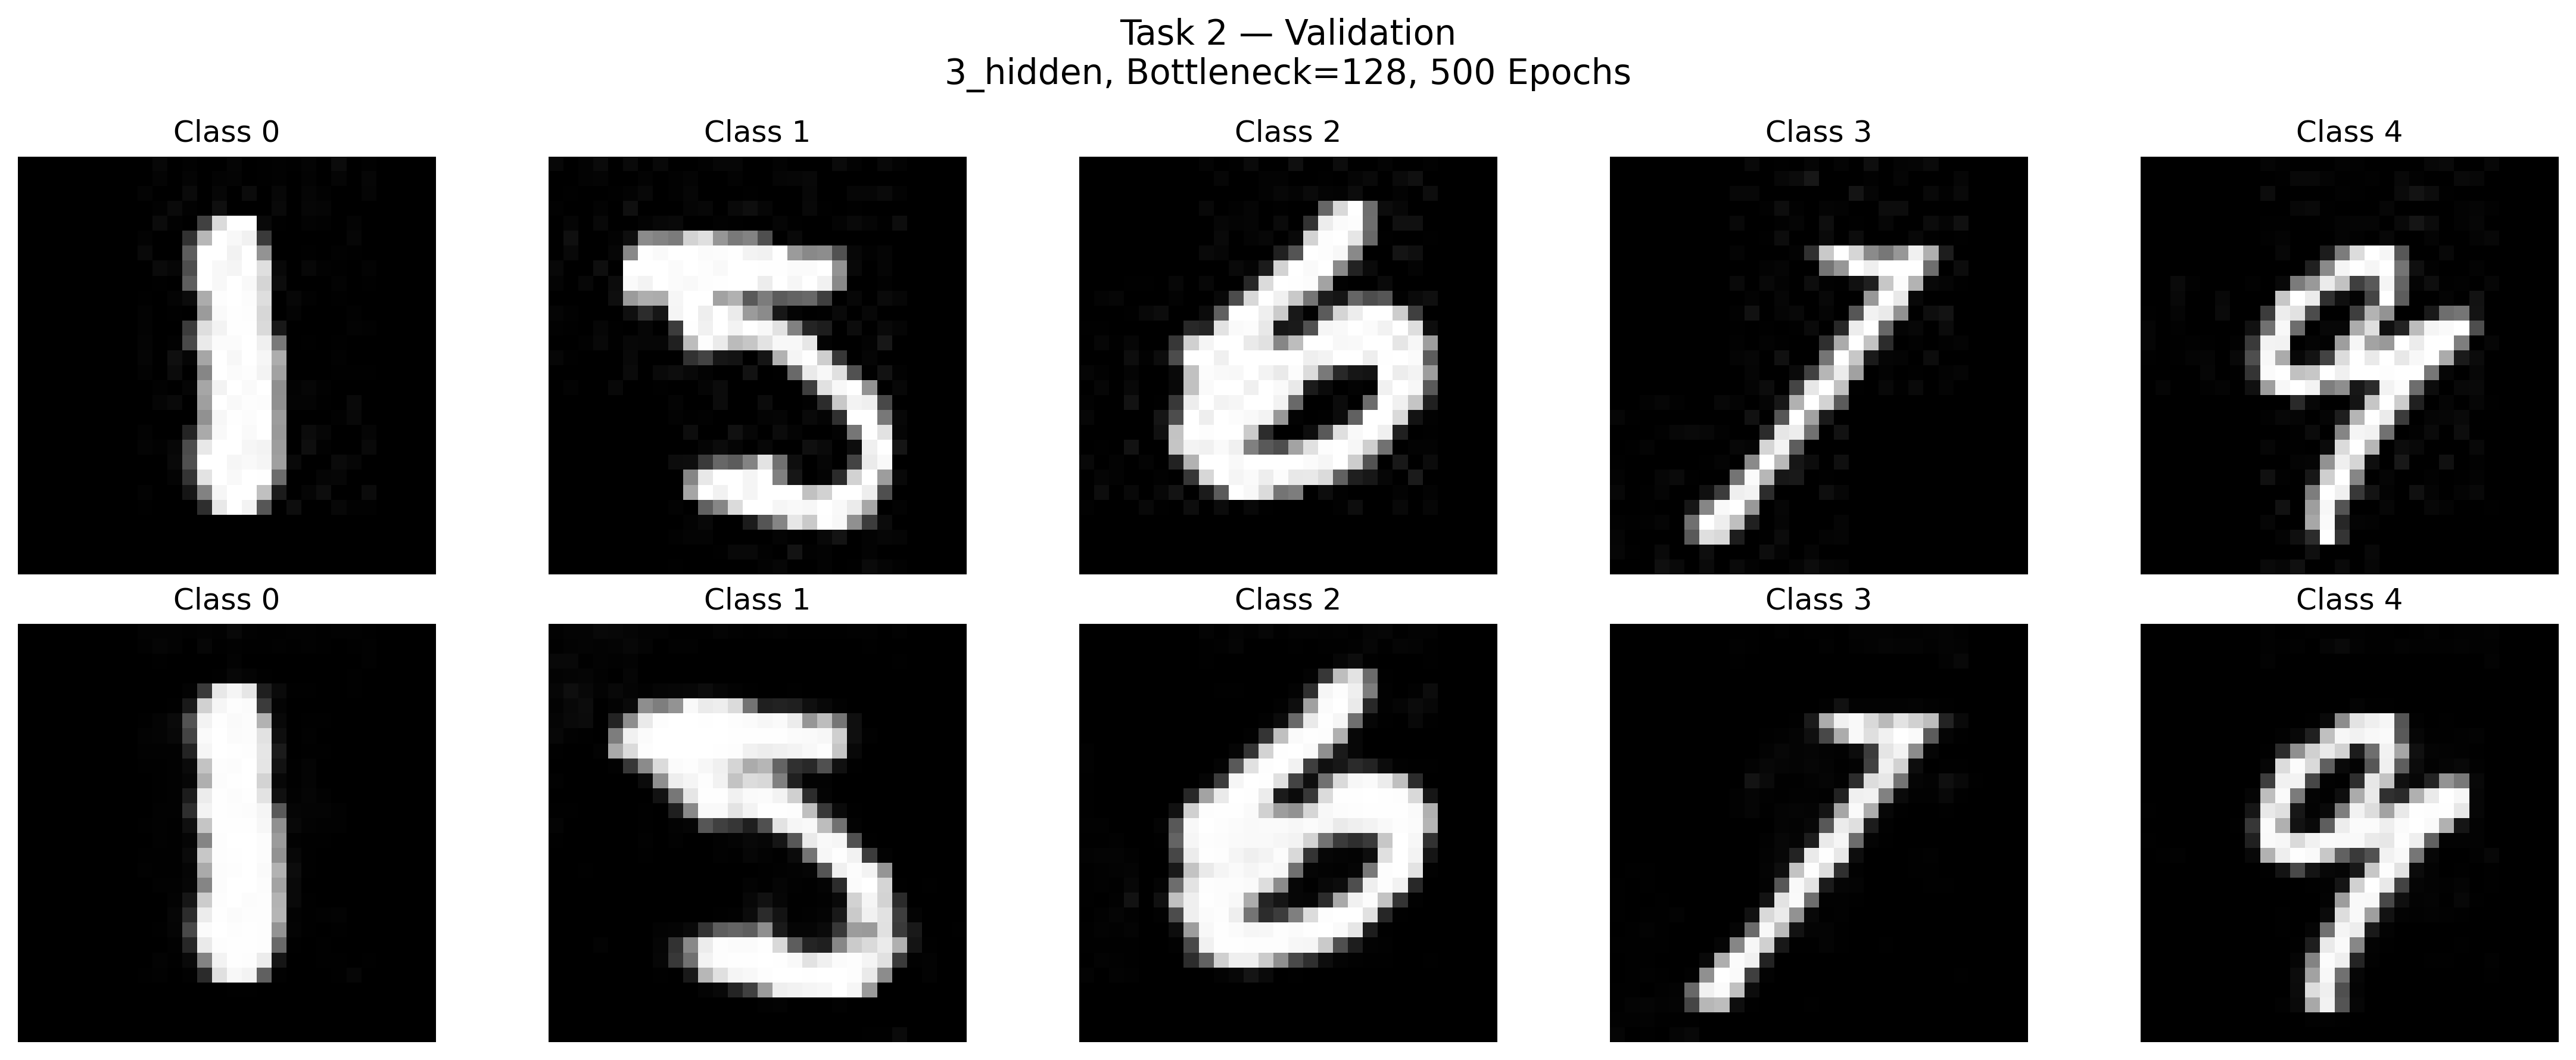
\includegraphics[width=0.96\linewidth,height=0.48\textheight,keepaspectratio]{figures/task2/model_reconstruction_visualization_500/validation_3_hidden_bottleneck_128_500epochs.png}
\caption{Autoencoder reconstruction visualization: validation 3 hidden with bottleneck of 128 neurons.}
\label{fig:task2_23}
\end{figure}

\begin{figure}[H]
\centering
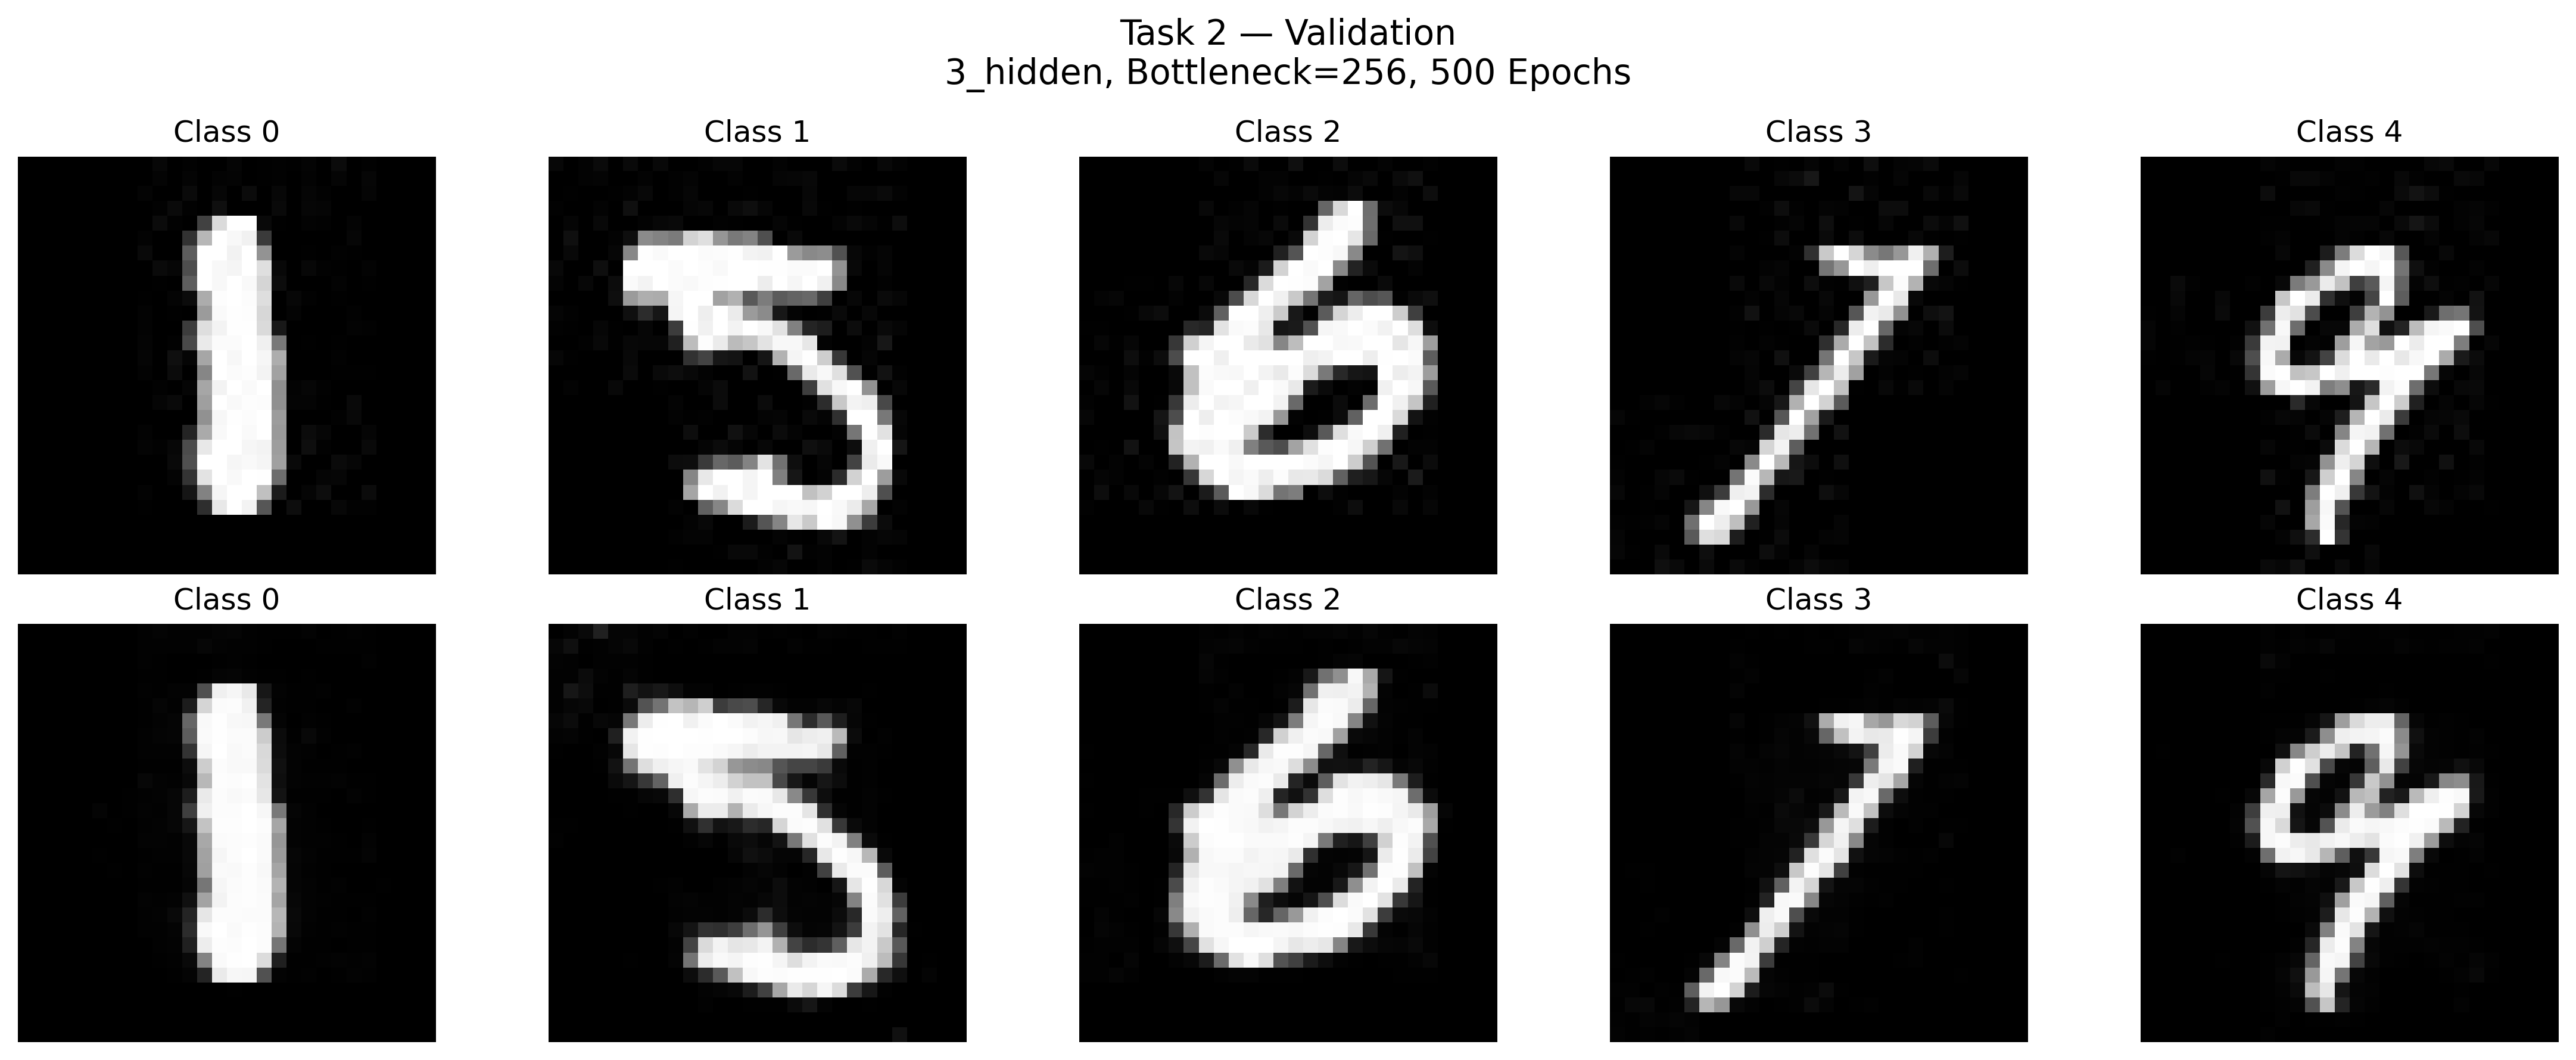
\includegraphics[width=0.96\linewidth,height=0.48\textheight,keepaspectratio]{figures/task2/model_reconstruction_visualization_500/validation_3_hidden_bottleneck_256_500epochs.png}
\caption{Autoencoder reconstruction visualization: validation 3 hidden with bottleneck of 256 neurons.}
\label{fig:task2_24}
\end{figure}

\FloatBarrier

\section{Task 3: Classification Using One-Hidden-Layer Autoencoder Representations}
\subsection{Method}
The encoder of each trained one-hidden-layer autoencoder is applied to the dataset to obtain 32-dimensional, 64-dimensional, 128-dimensional, or 256-dimensional features. The FCNN architectures are evaluated on these features, and validation accuracy is used to select the best architecture for each dimension.

\subsection{Results}
Table~\ref{tab:task3-results} shows that the 128-dimensional representation gives the highest test accuracy among the four dimensions, at 98.1555\%. The 64-dimensional representation is close at 98.1028\%, while the 32-dimensional and 256-dimensional representations are lower. Relative to Assignment 3 (98.1291\%) and the best PCA result in Task 1 (98.2345\%),
the best one-hidden-layer AE representation is 0.0264 percentage points above the
Assignment 3 baseline but 0.0790 percentage points below the PCA result. The AE
representation is therefore useful, but it does not surpass the best PCA classifier in
this experiment. This indicates that the representation with the largest number of latent features is not automatically the best for classification.

\begin{table}[H]
\centering
\small
\caption{Validation accuracy for every FCNN architecture and one-hidden-layer AE representation.}
\label{tab:task3-all-val}
\begin{tabular}{r l r}
\toprule
Representation dim. & FCNN architecture & Validation accuracy (\%)\\
\midrule
32 & 4\_hidden\_normal & 98.6825 \\
32 & 3\_hidden\_best & 98.6298 \\
32 & 4\_hidden\_best & 98.3663 \\
32 & 5\_hidden\_best & 97.9974 \\
64 & 4\_hidden\_best & 98.5507 \\
64 & 3\_hidden\_best & 98.4453 \\
64 & 4\_hidden\_normal & 98.3663 \\
64 & 5\_hidden\_best & 98.3399 \\
128 & 4\_hidden\_normal & 98.5244 \\
128 & 5\_hidden\_best & 98.4453 \\
128 & 4\_hidden\_best & 98.3663 \\
128 & 3\_hidden\_best & 98.2609 \\
256 & 5\_hidden\_best & 98.4453 \\
256 & 4\_hidden\_best & 98.2082 \\
256 & 4\_hidden\_normal & 98.1291 \\
256 & 3\_hidden\_best & 98.0237 \\
\bottomrule
\end{tabular}
\end{table}

\begin{table}[H]
\centering
\small
\caption{Best classification result by one-hidden-layer AE representation.}
\label{tab:task3-results}
\begin{tabular}{r l r r}
\toprule
Dim. & Architecture & Val. acc. (\%) & Test acc. (\%)\\
\midrule
32 & 4-hidden normal & 98.6825 & 97.9447\\
64 & 4-hidden best & 98.5507 & 98.1028\\
128 & 4-hidden normal & 98.5244 & 98.1555\\
256 & 5-hidden best & 98.4453 & 97.9974\\
\bottomrule
\end{tabular}
\end{table}

The confusion matrices provide additional detail on the errors made by the best classifier for each latent dimension.

% Automatically generated figure inventory for task3.

\begin{figure}[H]
\centering
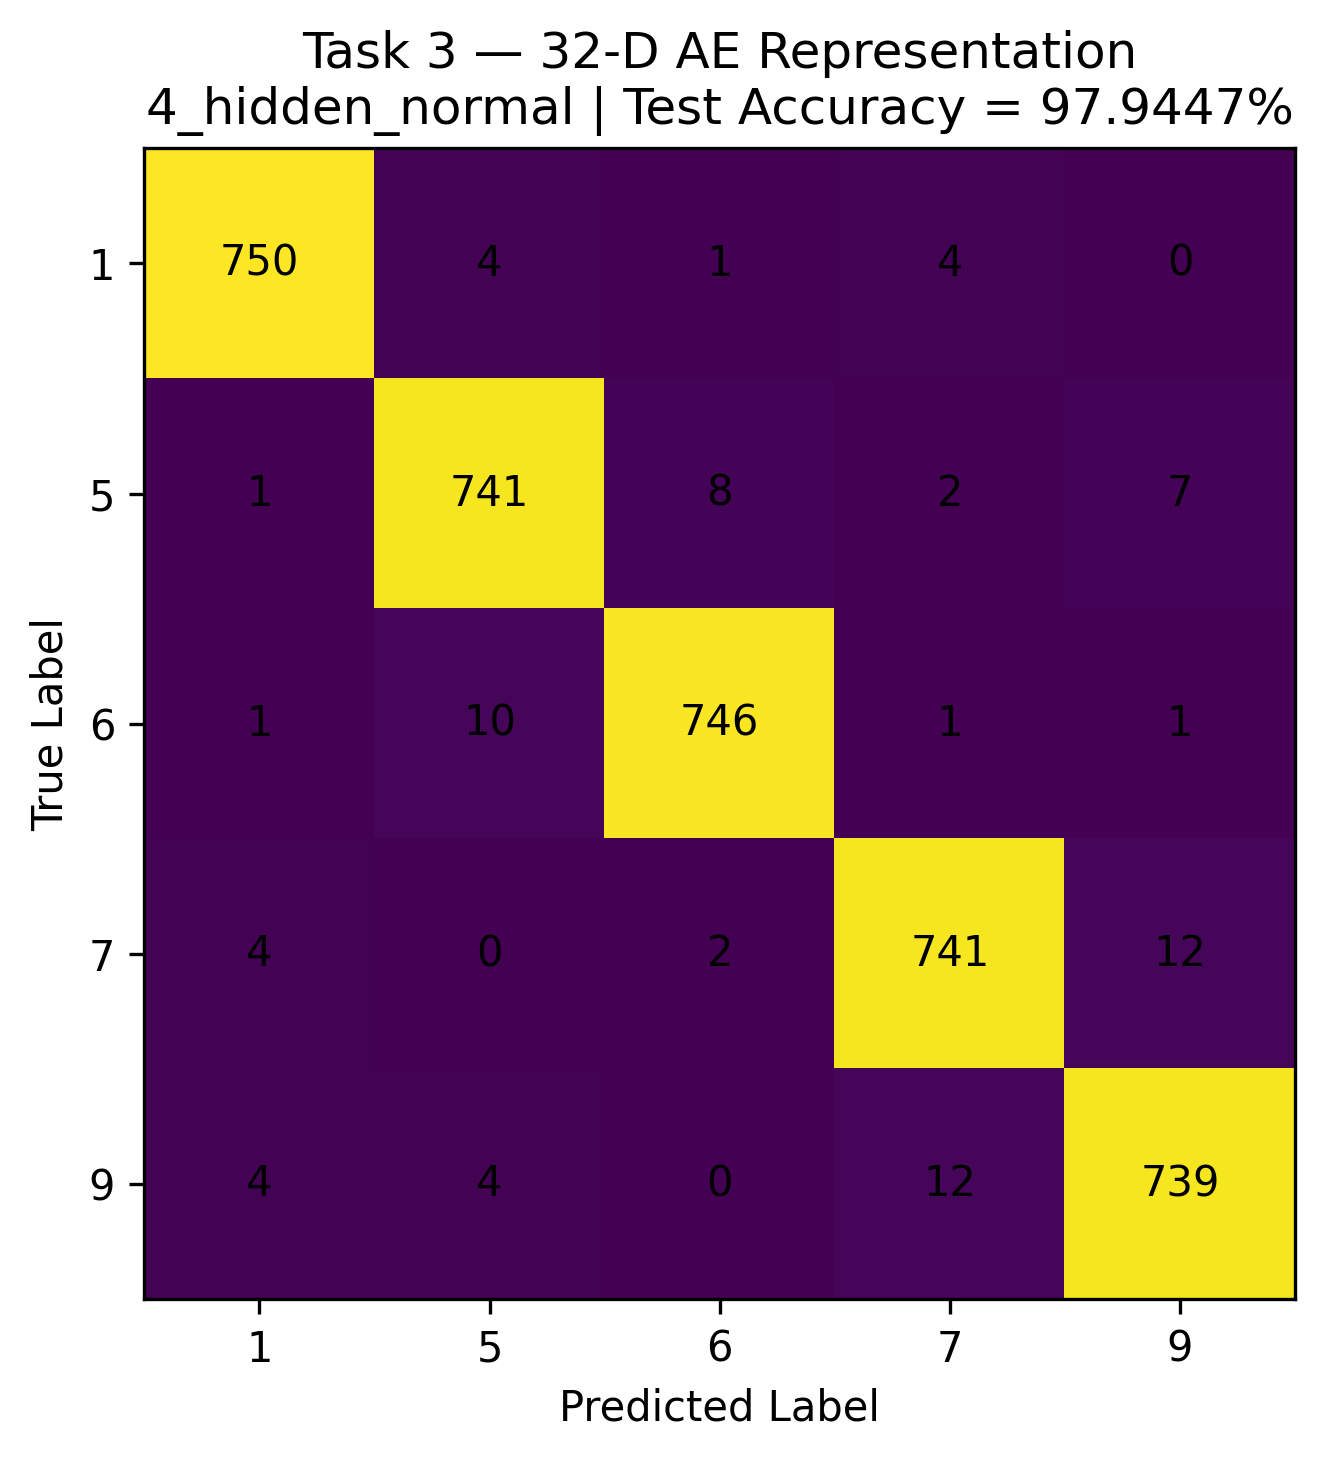
\includegraphics[width=0.88\linewidth,height=0.34\textheight,keepaspectratio]{figures/task3/cnf_matrics_img/confusion_matrix_32.png}
\caption{Confusion matrix: confusion matrix for 32 neurons bottleneck.}
\label{fig:task3_1}
\end{figure}

\begin{figure}[H]
\centering
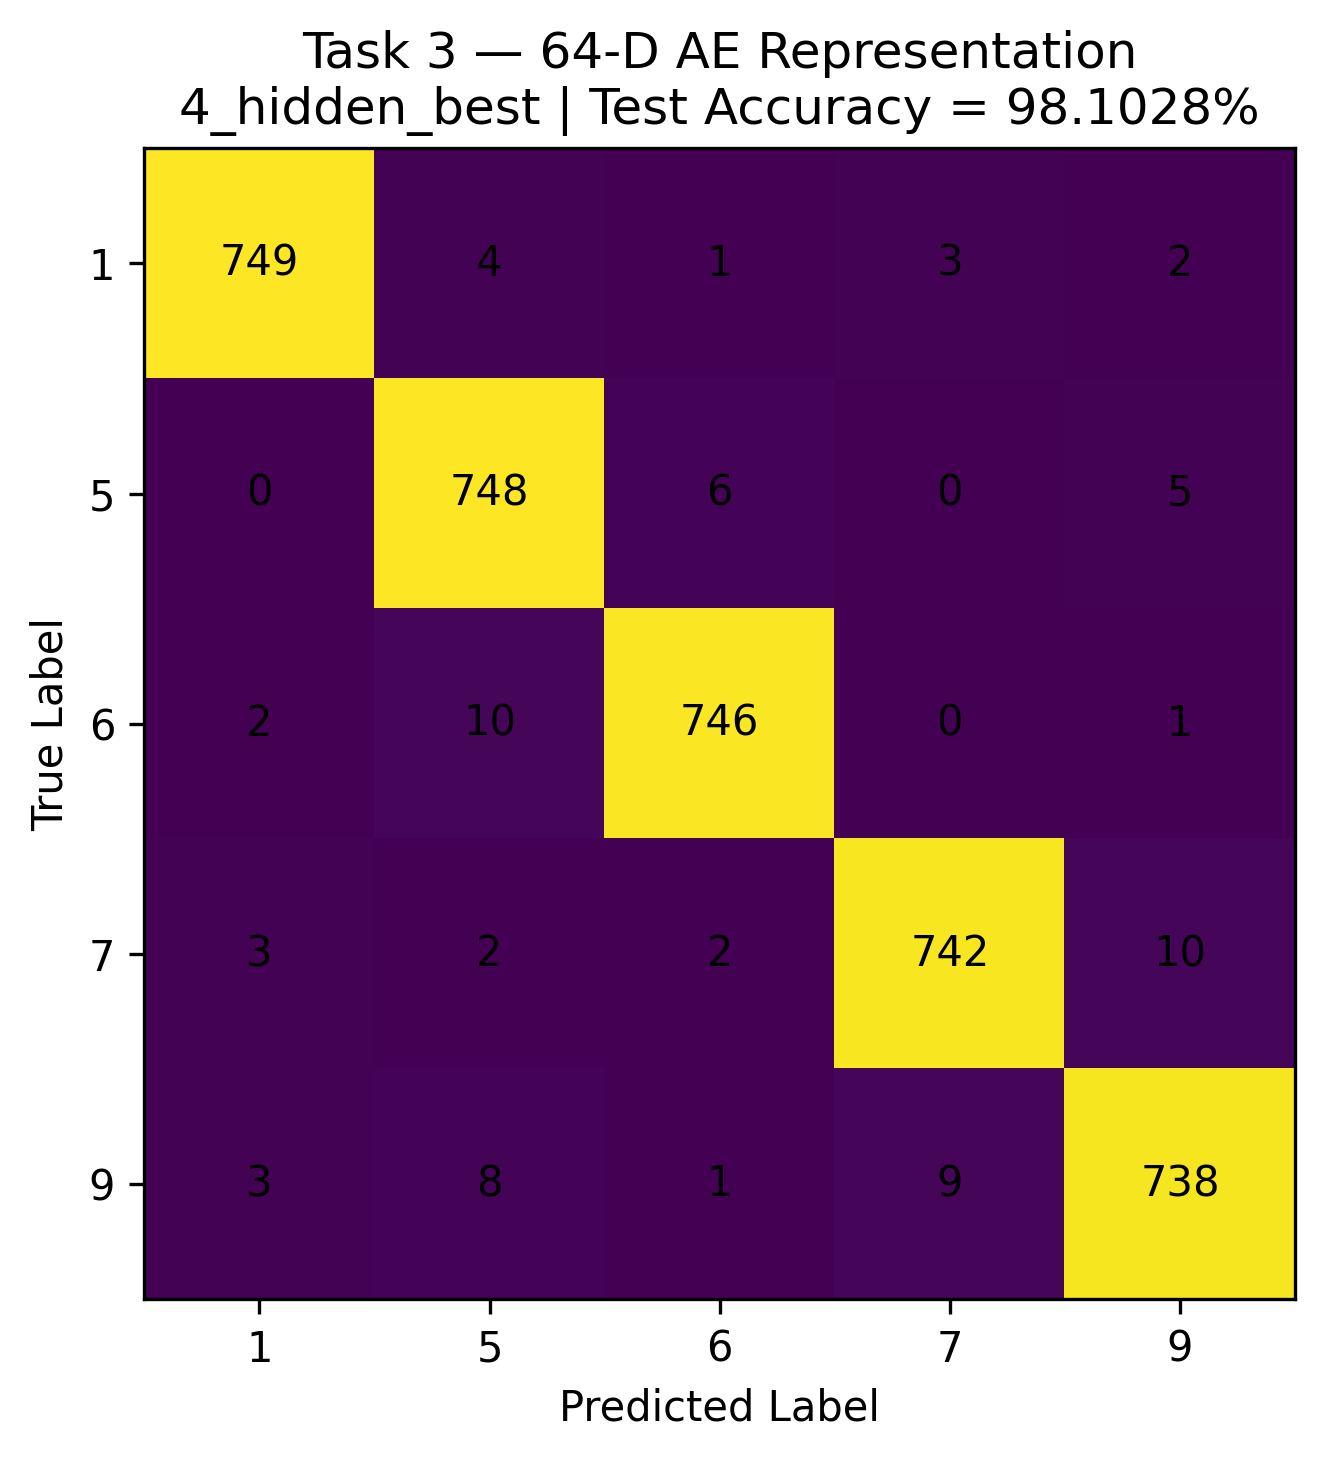
\includegraphics[width=0.88\linewidth,height=0.34\textheight,keepaspectratio]{figures/task3/cnf_matrics_img/confusion_matrix_64.png}
\caption{Confusion matrix: confusion matrix for 64 neurons bottleneck.}
\label{fig:task3_2}
\end{figure}

\begin{figure}[H]
\centering
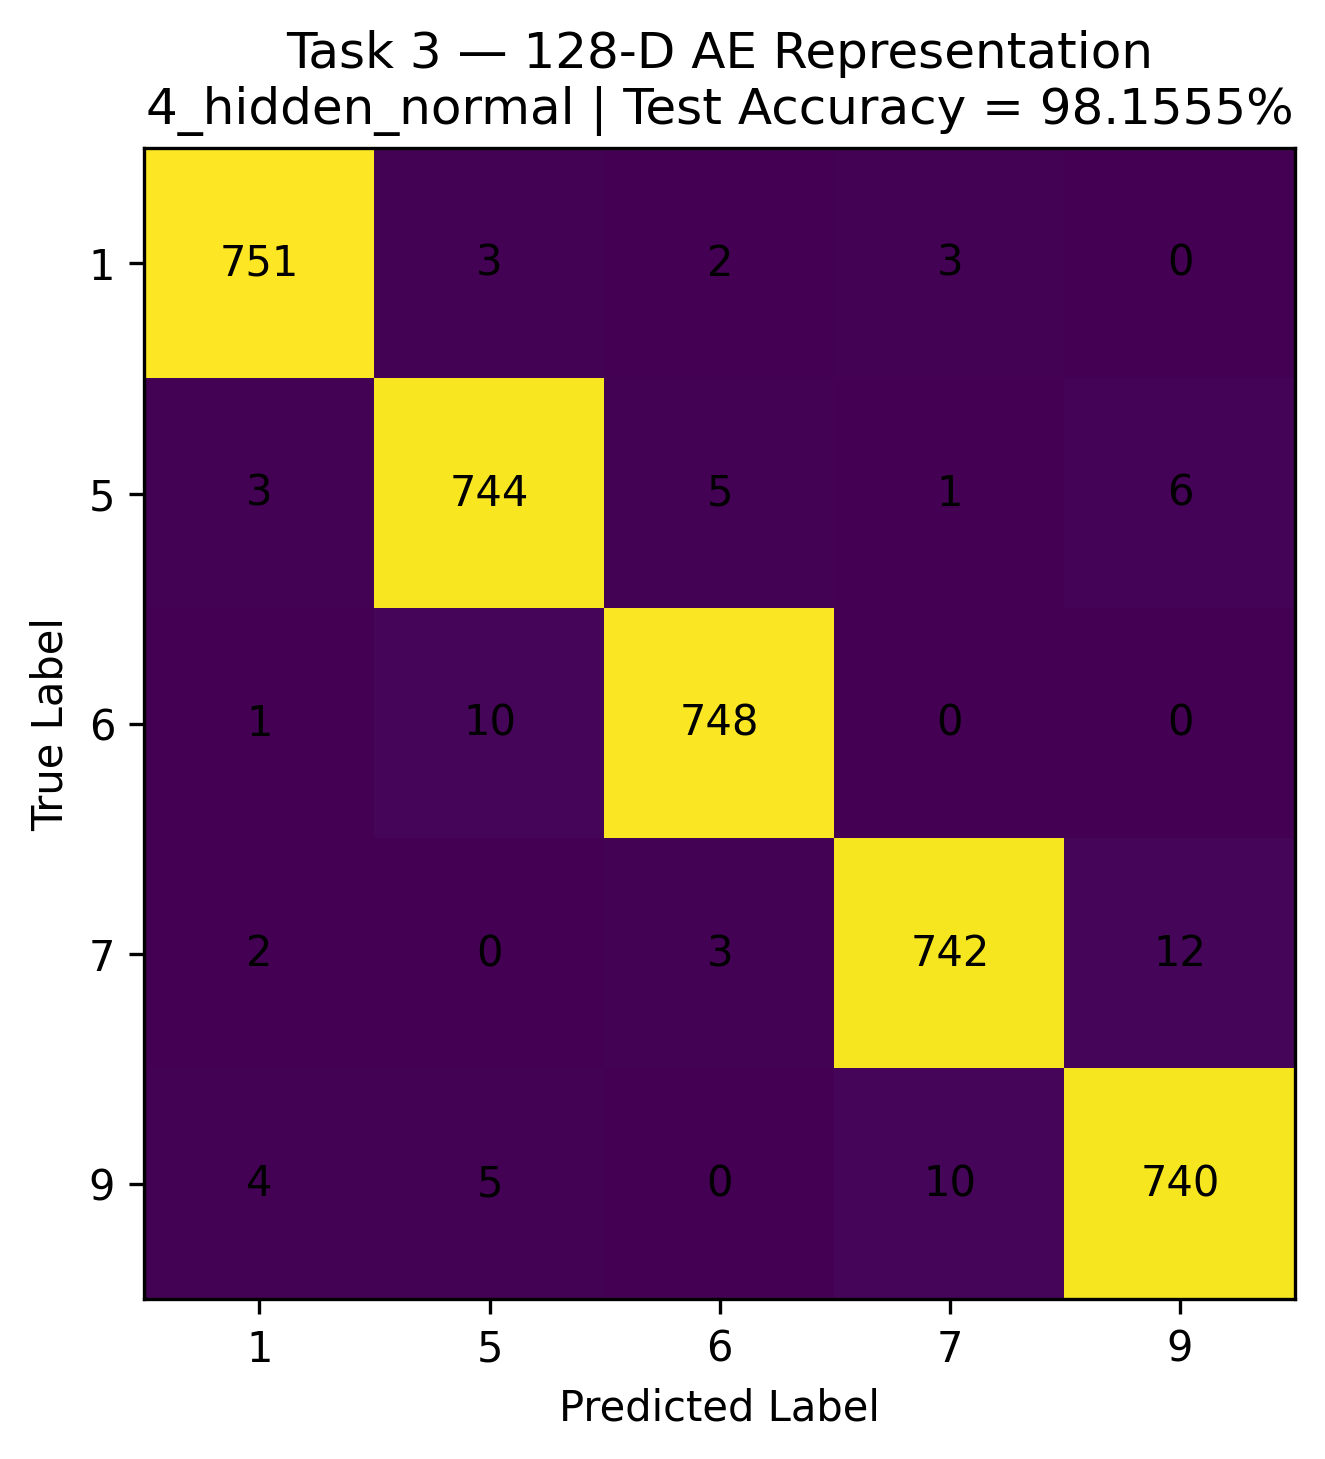
\includegraphics[width=0.88\linewidth,height=0.34\textheight,keepaspectratio]{figures/task3/cnf_matrics_img/confusion_matrix_128.png}
\caption{Confusion matrix: confusion matrix for 128 neurons bottleneck.}
\label{fig:task3_3}
\end{figure}

\begin{figure}[H]
\centering
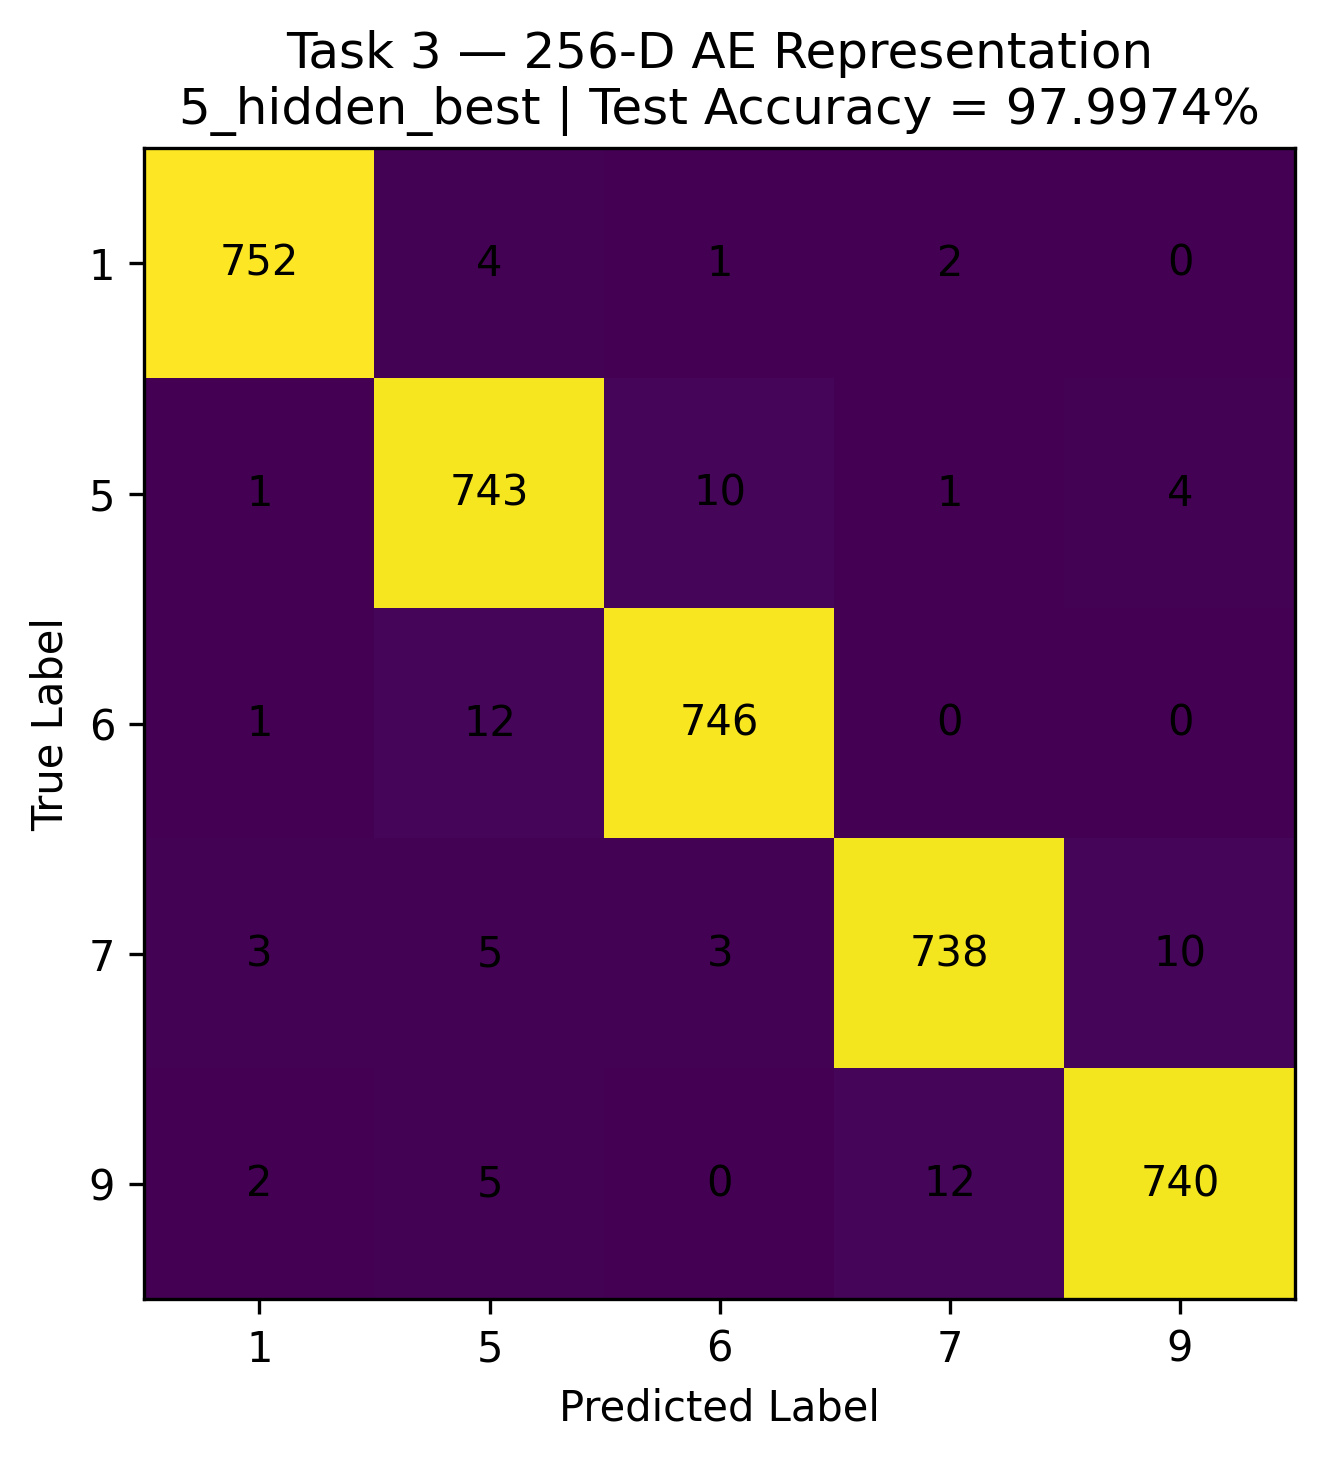
\includegraphics[width=0.88\linewidth,height=0.34\textheight,keepaspectratio]{figures/task3/cnf_matrics_img/confusion_matrix_256.png}
\caption{Confusion matrix: confusion matrix for 256 neurons bottleneck.}
\label{fig:task3_4}
\end{figure}

\FloatBarrier

\section{Task 4: Classification Using Three-Hidden-Layer Autoencoder Representations}
\subsection{Encoder representation}
For this task, the encoder portion of the three-hidden-layer autoencoder is used up to and including the bottleneck. The resulting representations have dimensions 32, 64, 128, and 256. The same set of FCNN architectures and validation-based selection procedure is applied to each representation.

\subsection{Results}
The 64-dimensional representation produces the best test accuracy, 98.2872\%, using the five-hidden-layer FCNN configuration. The 32-dimensional representation reaches 98.2345\%, whereas the 128- and 256-dimensional representations are lower. Compared with Assignment 3 (98.1291\%), Task 1 PCA (98.2345\%), and Task 3
(one-hidden-layer AE, 98.1555\%), the 64-D three-hidden-layer AE encoder is best among
these four methods at 98.2872\%. It exceeds the Assignment 3 baseline by 0.1581
percentage points, PCA by 0.0527 percentage points, and Task 3 by 0.1317 percentage
points. The results again show that the best representation dimension is determined empirically and need not be the largest.

\begin{table}[H]
\centering
\small
\caption{Validation accuracy for every FCNN architecture and three-hidden-layer AE representation.}
\label{tab:task4-all-val}
\begin{tabular}{r l r}
\toprule
Representation dim. & FCNN architecture & Validation accuracy (\%)\\
\midrule
32 & 3\_hidden\_best & 98.6034 \\
32 & 4\_hidden\_best & 98.5507 \\
32 & 4\_hidden\_normal & 98.5507 \\
32 & 5\_hidden\_best & 98.7615 \\
64 & 3\_hidden\_best & 98.4190 \\
64 & 4\_hidden\_best & 98.3399 \\
64 & 4\_hidden\_normal & 98.3663 \\
64 & 5\_hidden\_best & 98.4453 \\
128 & 3\_hidden\_best & 98.1555 \\
128 & 4\_hidden\_best & 98.3136 \\
128 & 4\_hidden\_normal & 98.4453 \\
128 & 5\_hidden\_best & 98.3136 \\
256 & 3\_hidden\_best & 98.1028 \\
256 & 4\_hidden\_best & 98.4717 \\
256 & 4\_hidden\_normal & 98.2082 \\
256 & 5\_hidden\_best & 98.2345 \\
\bottomrule
\end{tabular}
\end{table}

\begin{table}[H]
\centering
\small
\caption{Best classification result by three-hidden-layer AE representation.}
\label{tab:task4-results}
\begin{tabular}{r l r r}
\toprule
Dim. & Architecture & Val. acc. (\%) & Test acc. (\%)\\
\midrule
32 & 5-hidden best & 98.7615 & 98.2345\\
64 & 5-hidden best & 98.4453 & 98.2872\\
128 & 4-hidden normal & 98.4453 & 97.8393\\
256 & 4-hidden best & 98.4717 & 97.9183\\
\bottomrule
\end{tabular}
\end{table}

The confusion matrices for the four dimensions are shown next.

% Automatically generated figure inventory for task4.

\begin{figure}[H]
\centering
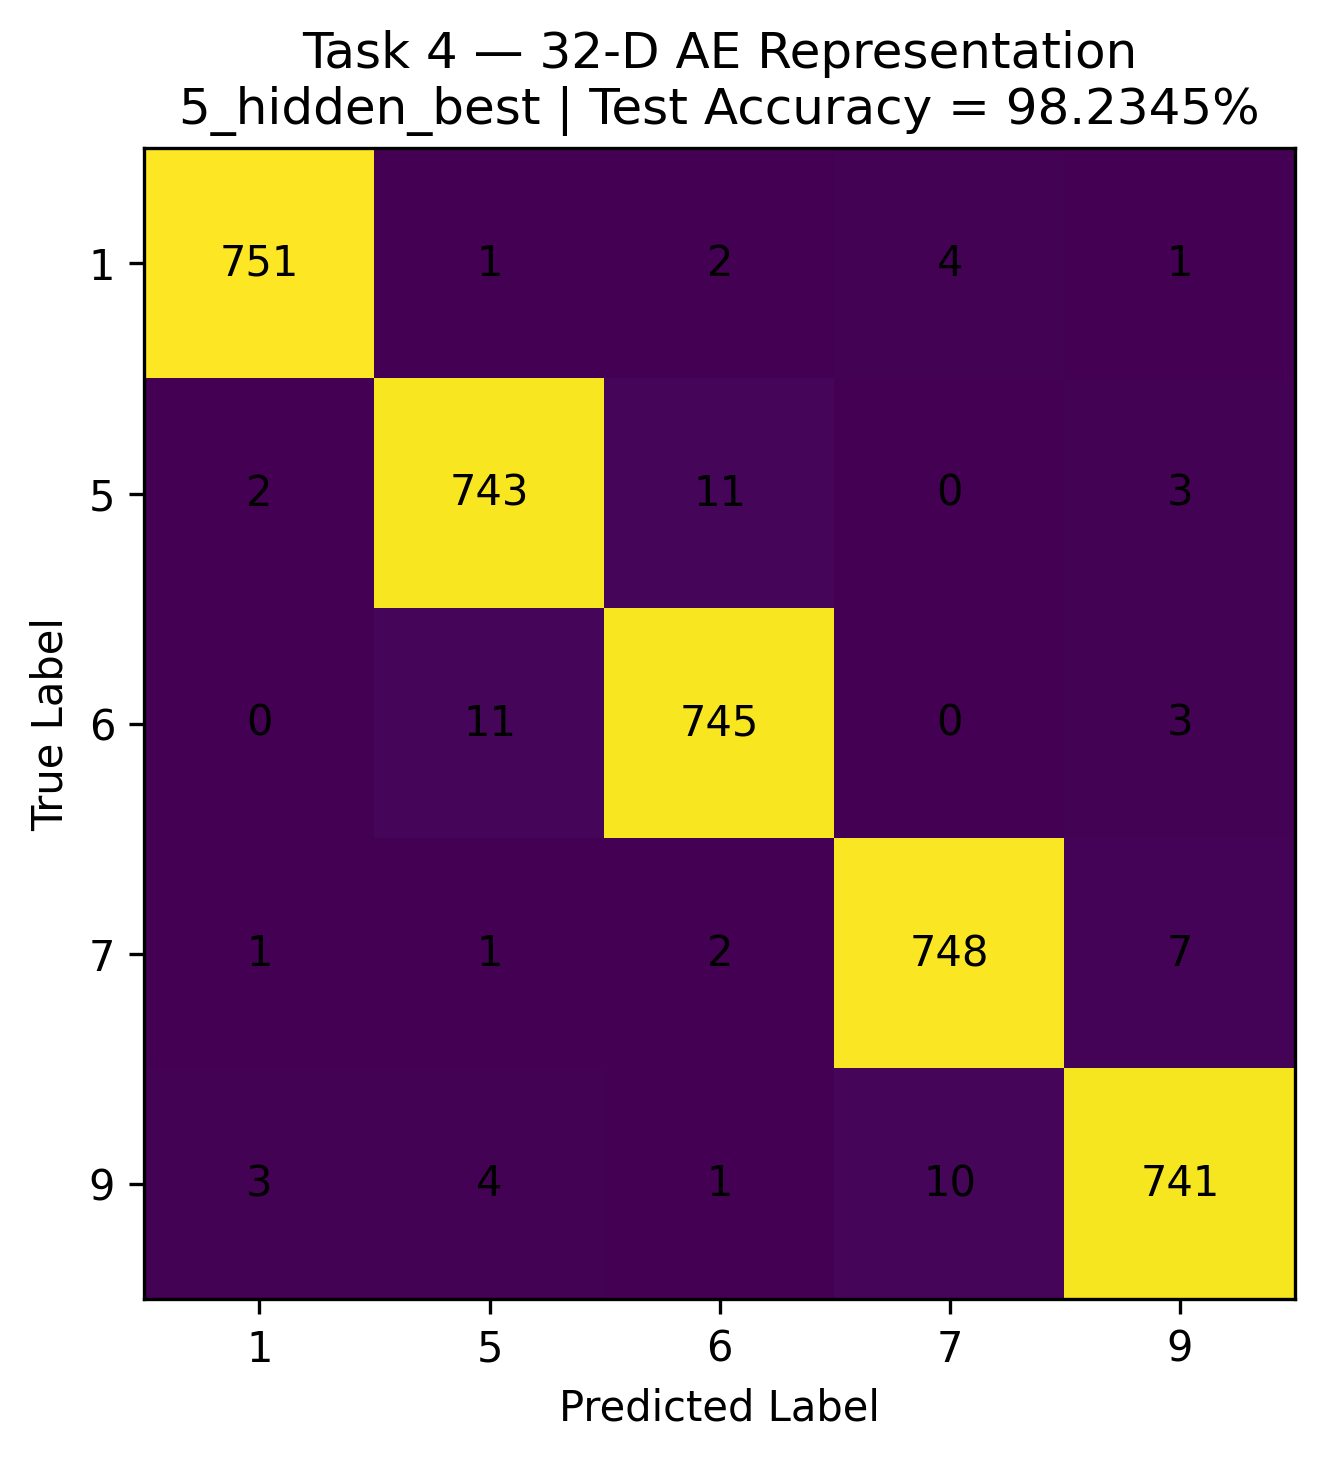
\includegraphics[width=0.88\linewidth,height=0.34\textheight,keepaspectratio]{figures/task4/cnf_img/confusion_matrix_32.png}
\caption{Confusion matrix: confusion matrix for 32 neurons bottleneck.}
\label{fig:task4_1}
\end{figure}

\begin{figure}[H]
\centering
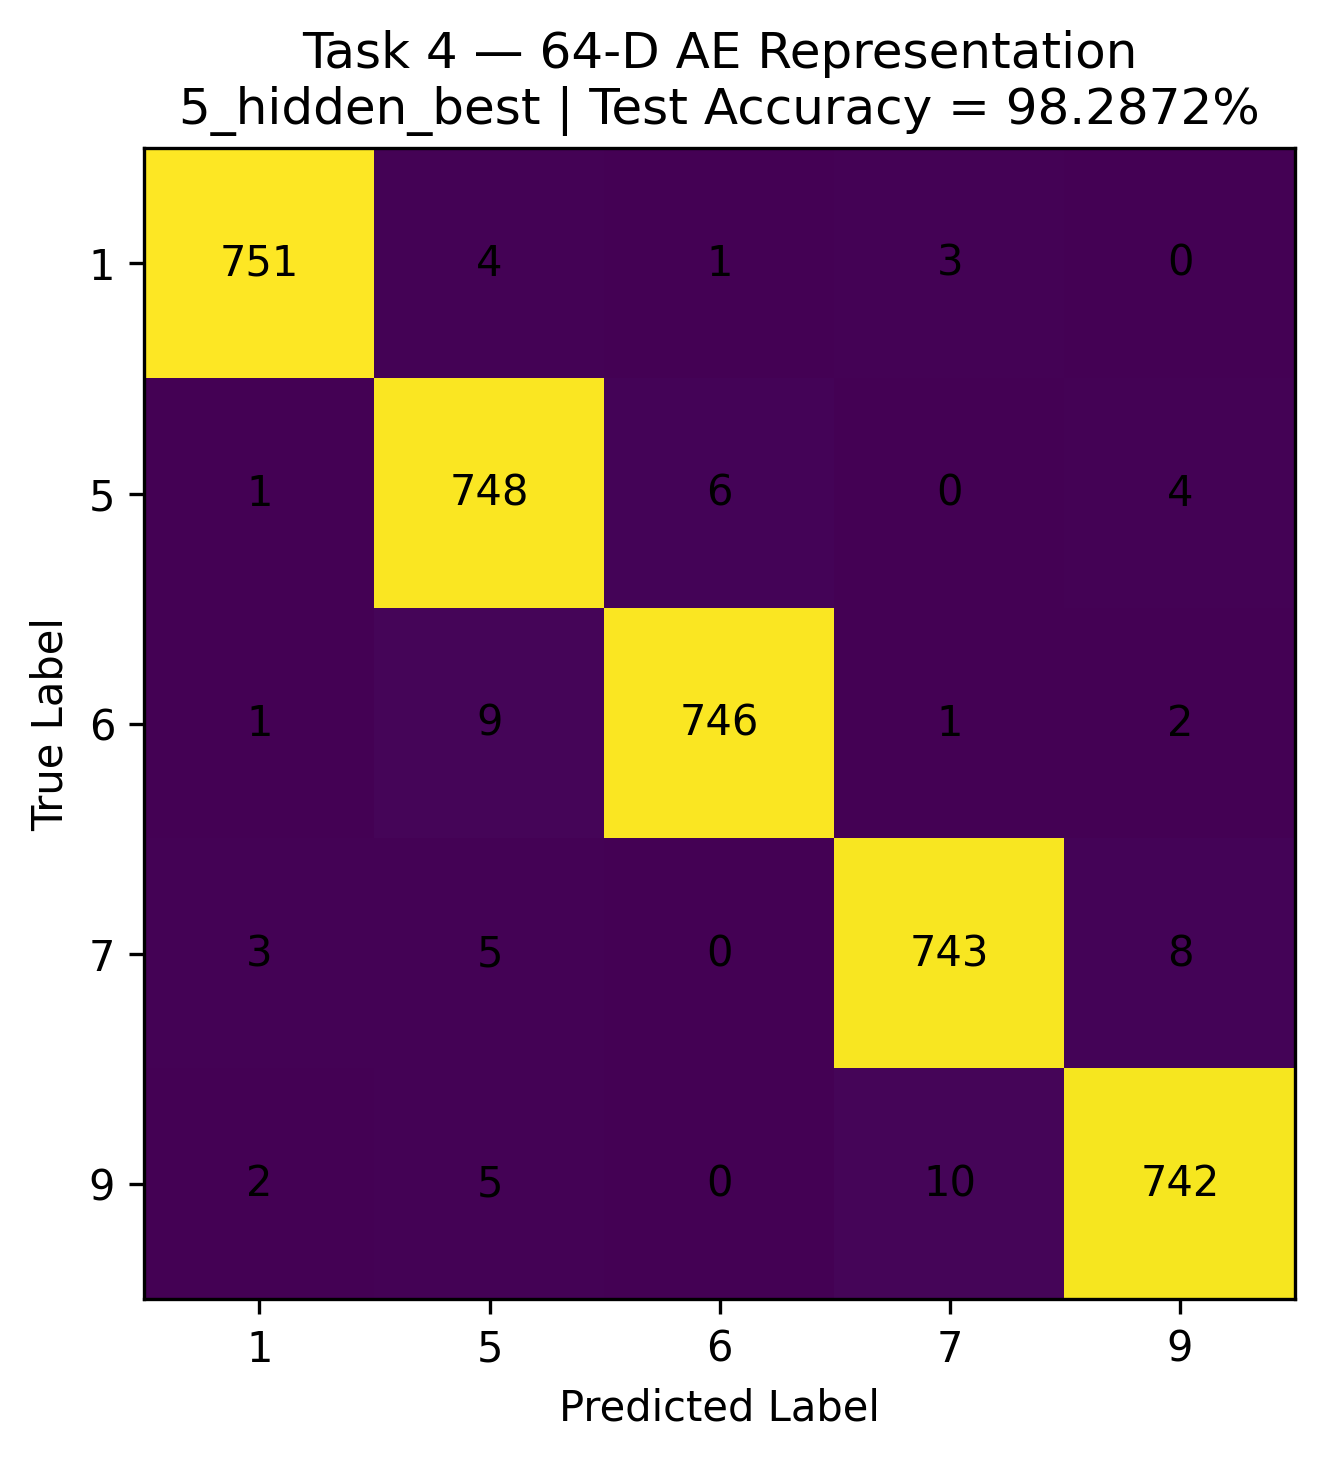
\includegraphics[width=0.88\linewidth,height=0.34\textheight,keepaspectratio]{figures/task4/cnf_img/confusion_matrix_64.png}
\caption{Confusion matrix: confusion matrix for 64 neurons bottleneck.}
\label{fig:task4_2}
\end{figure}

\begin{figure}[H]
\centering
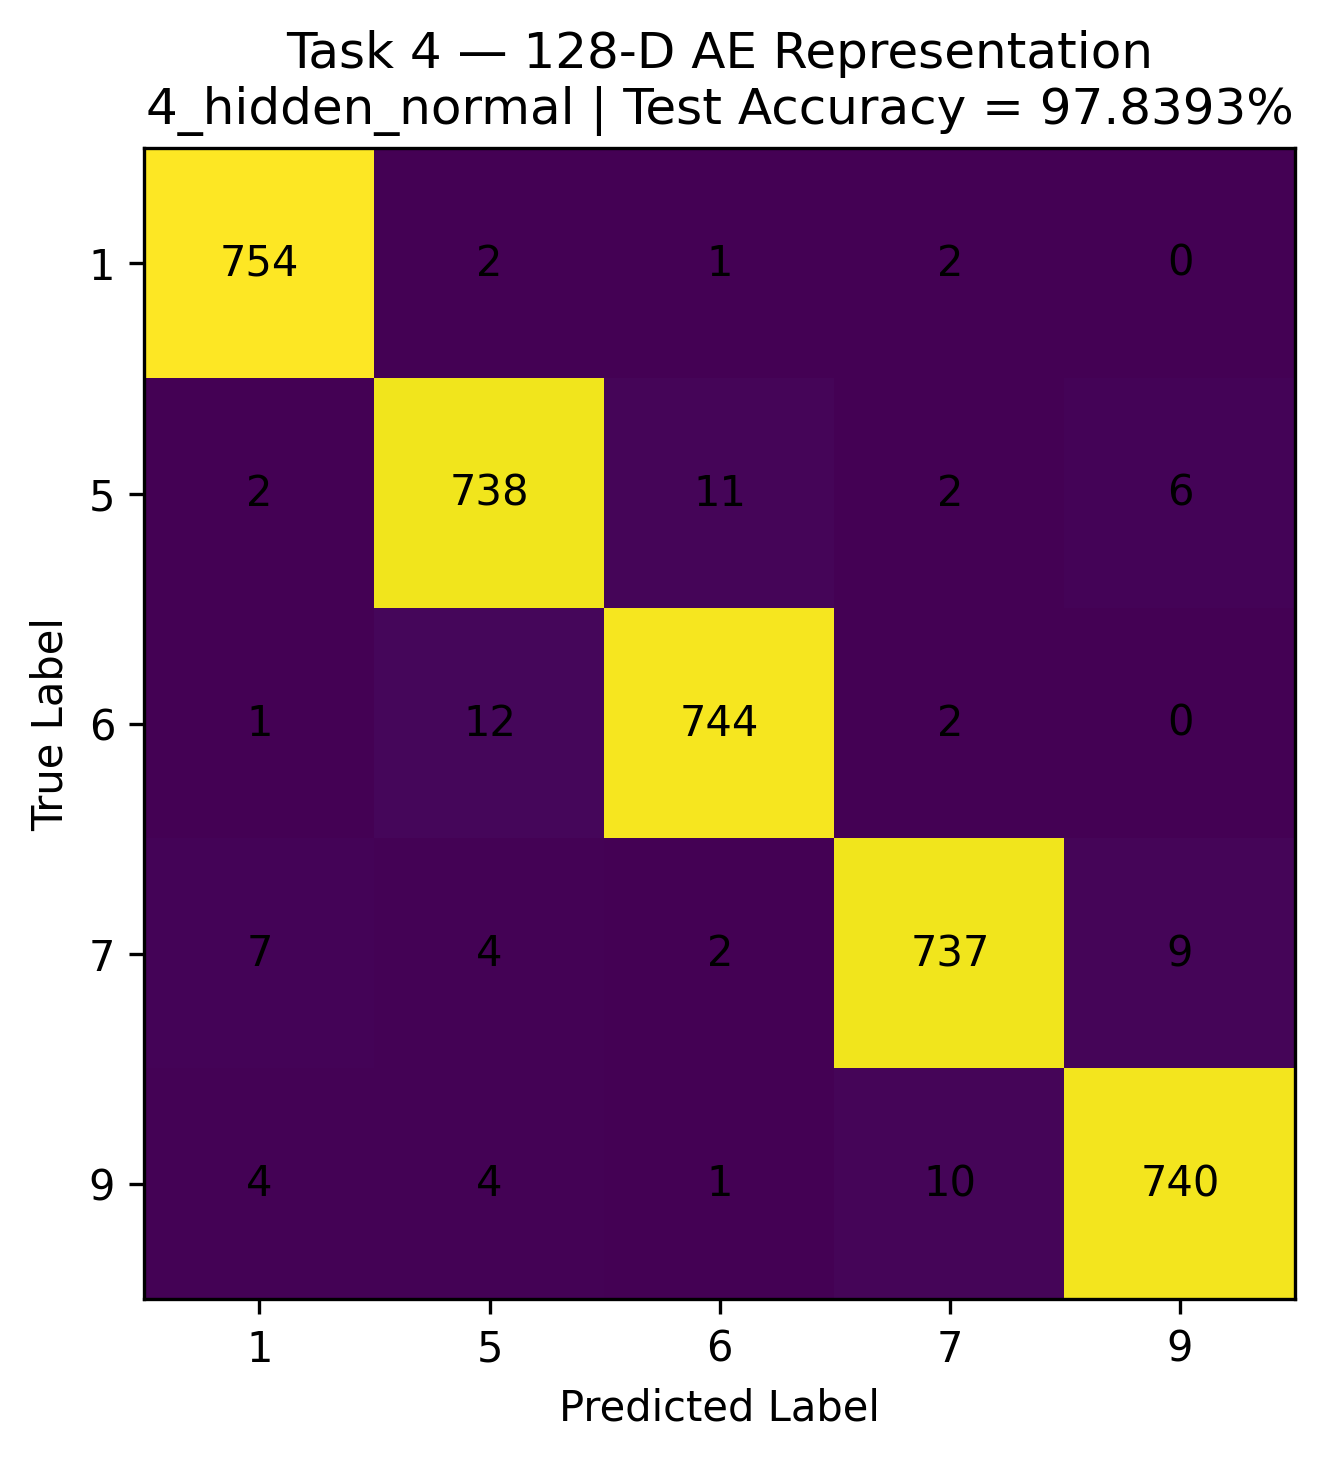
\includegraphics[width=0.88\linewidth,height=0.34\textheight,keepaspectratio]{figures/task4/cnf_img/confusion_matrix_128.png}
\caption{Confusion matrix: confusion matrix for 128 neurons bottleneck.}
\label{fig:task4_3}
\end{figure}

\begin{figure}[H]
\centering
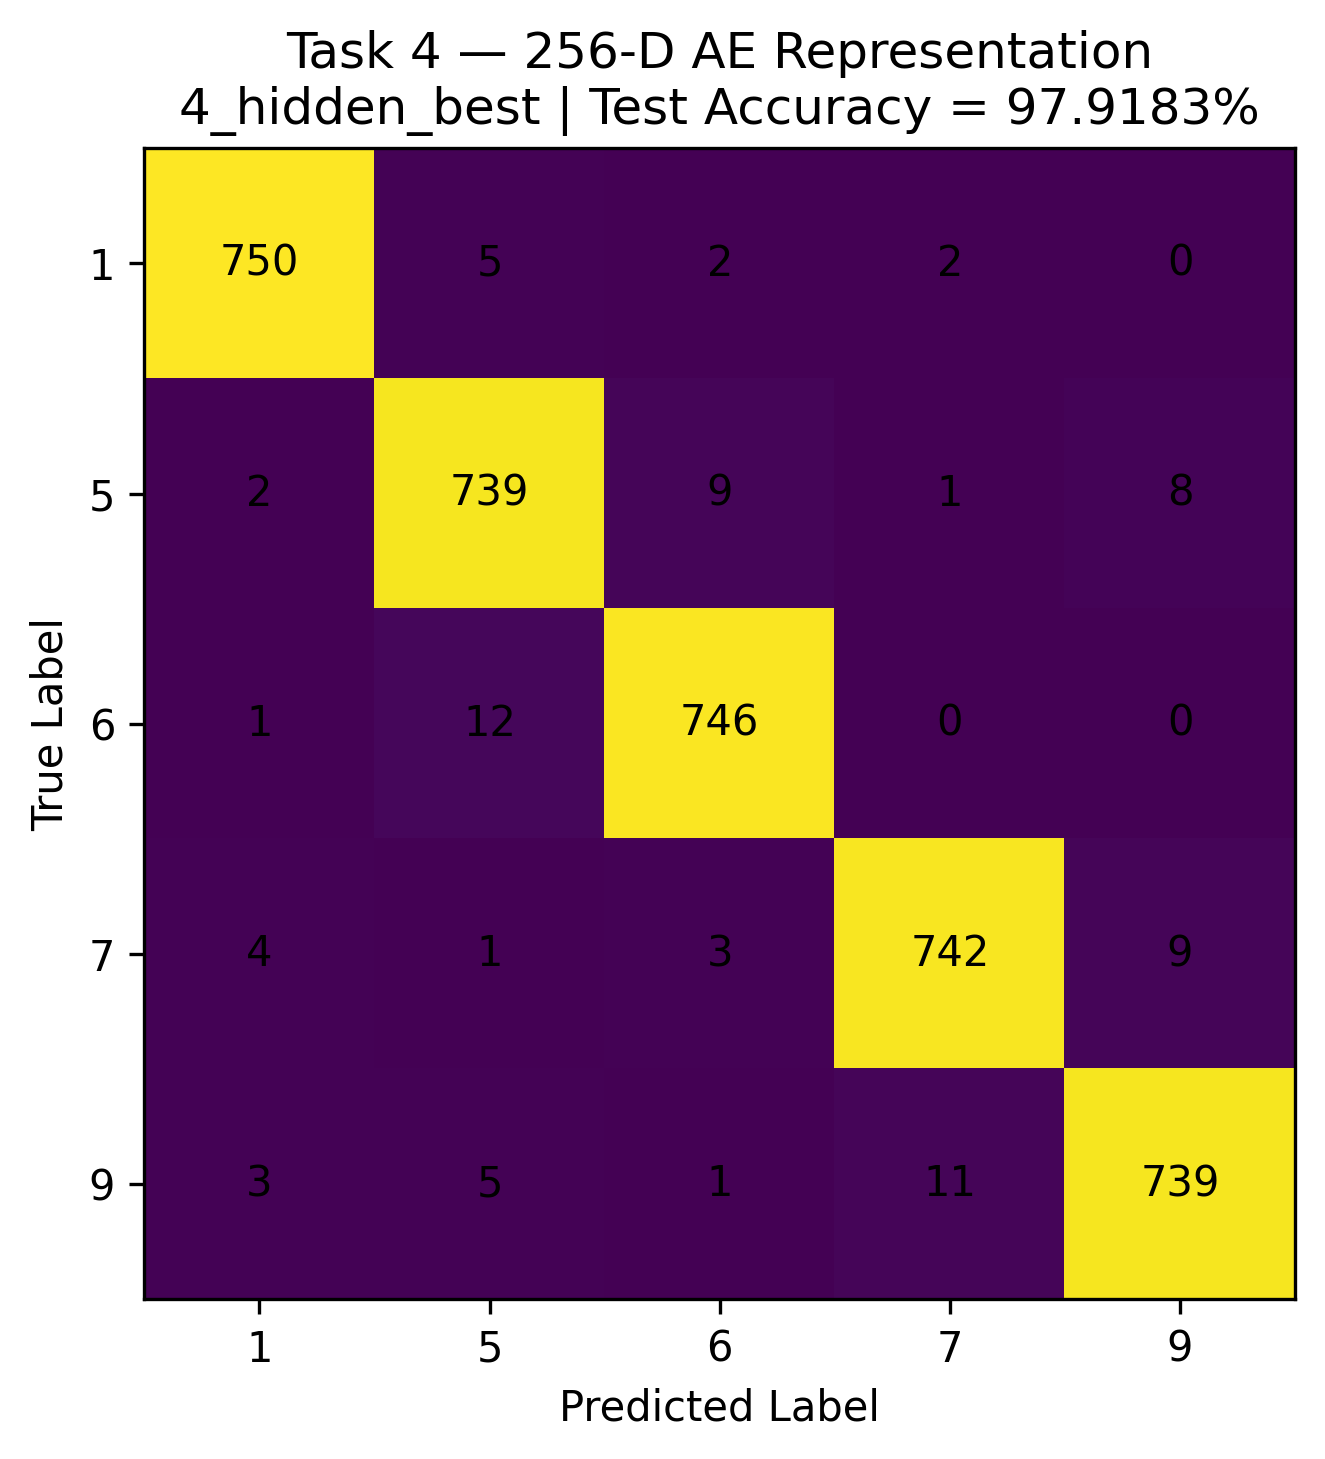
\includegraphics[width=0.88\linewidth,height=0.34\textheight,keepaspectratio]{figures/task4/cnf_img/confusion_matrix_256.png}
\caption{Confusion matrix: confusion matrix for 256 neurons bottleneck.}
\label{fig:task4_4}
\end{figure}

\FloatBarrier

\section{Task 5: Denoising Autoencoders}
\subsection{Noise model and evaluation}
One-hidden-layer denoising autoencoders (DAEs) are evaluated using 20\% and 40\% corruption, with the bottleneck dimension fixed at 128. Gaussian noise is sampled from a standard normal distribution, $\epsilon\sim
\mathcal{N}(0,1)$. A Bernoulli mask $m_i\sim\operatorname{Bernoulli}(q)$ selects
pixels to corrupt, where $q\in\{0.20,0.40\}$. The noisy input used in the notebook is
\begin{equation}
\tilde{x}_i=x_i+m_i\epsilon_i,\qquad
\epsilon_i\sim\mathcal{N}(0,1),\quad m_i\sim\operatorname{Bernoulli}(q).
\end{equation}
This corresponds to the code that samples a random mask and uses \texttt{torch.randn\_like}
for the $N(0,1)$ noise. The target remains the clean input $x$. The autoencoders are trained to reconstruct clean inputs from corrupted inputs. Both reconstruction MSE and downstream classification accuracy are reported. The
denoising autoencoders are trained for up to 500 epochs with Adam (learning rate
$0.001$, batch size $128$). Their downstream FCNN uses the best Task 3 architecture for
the 128-D representation, namely \texttt{4\_hidden\_normal} with hidden widths
$[256,128,64,32]$, trained with SGD with momentum ($\eta=0.001$, $\mu=0.9$,
batch size $1$) and the same FCNN convergence criterion.

\subsection{Reconstruction results}
Table~\ref{tab:dae-mse} shows that the 20\% noise model has lower reconstruction MSE than the 40\% noise model on all three splits. The increase in error with stronger corruption is consistent with the more difficult reconstruction problem.

\begin{table}[H]
\centering
\caption{Task 5: Denoising reconstruction MSE.}
\label{tab:dae-mse}
\begin{tabular}{l r r r}
\toprule
Noise level & Train MSE & Val. MSE & Test MSE\\
\midrule
20\% & 0.010297 & 0.010644 & 0.010699\\
40\% & 0.015991 & 0.016365 & 0.016454\\
\bottomrule
\end{tabular}
\end{table}

\subsection{Classification results}
Both denoising representations are classified using the 128-dimensional feature setup and the \texttt{4\_hidden\_normal} architecture. The 20\% DAE achieves 98.4453\% test accuracy, and the 40\% DAE achieves 98.4190\%. The 20\% DAE therefore gives the stronger classification result in this comparison. Notably, reconstruction MSE and classification accuracy measure different objectives: the model with lower reconstruction error is not necessarily the model with the best downstream classification result across all tasks.

\begin{table}[H]
\centering
\caption{DAE classification results.}
\label{tab:dae-cls}
\begin{tabular}{l r r}
\toprule
Noise level & Val. acc. (\%) & Test acc. (\%)\\
\midrule
20\% & 98.5771 & 98.4453\\
40\% & 98.5507 & 98.4190\\
\bottomrule
\end{tabular}
\end{table}

The following figures include the classification confusion matrices and reconstruction examples for both noise levels and all supplied splits.

% Automatically generated figure inventory for task5.

\begin{figure}[H]
\centering
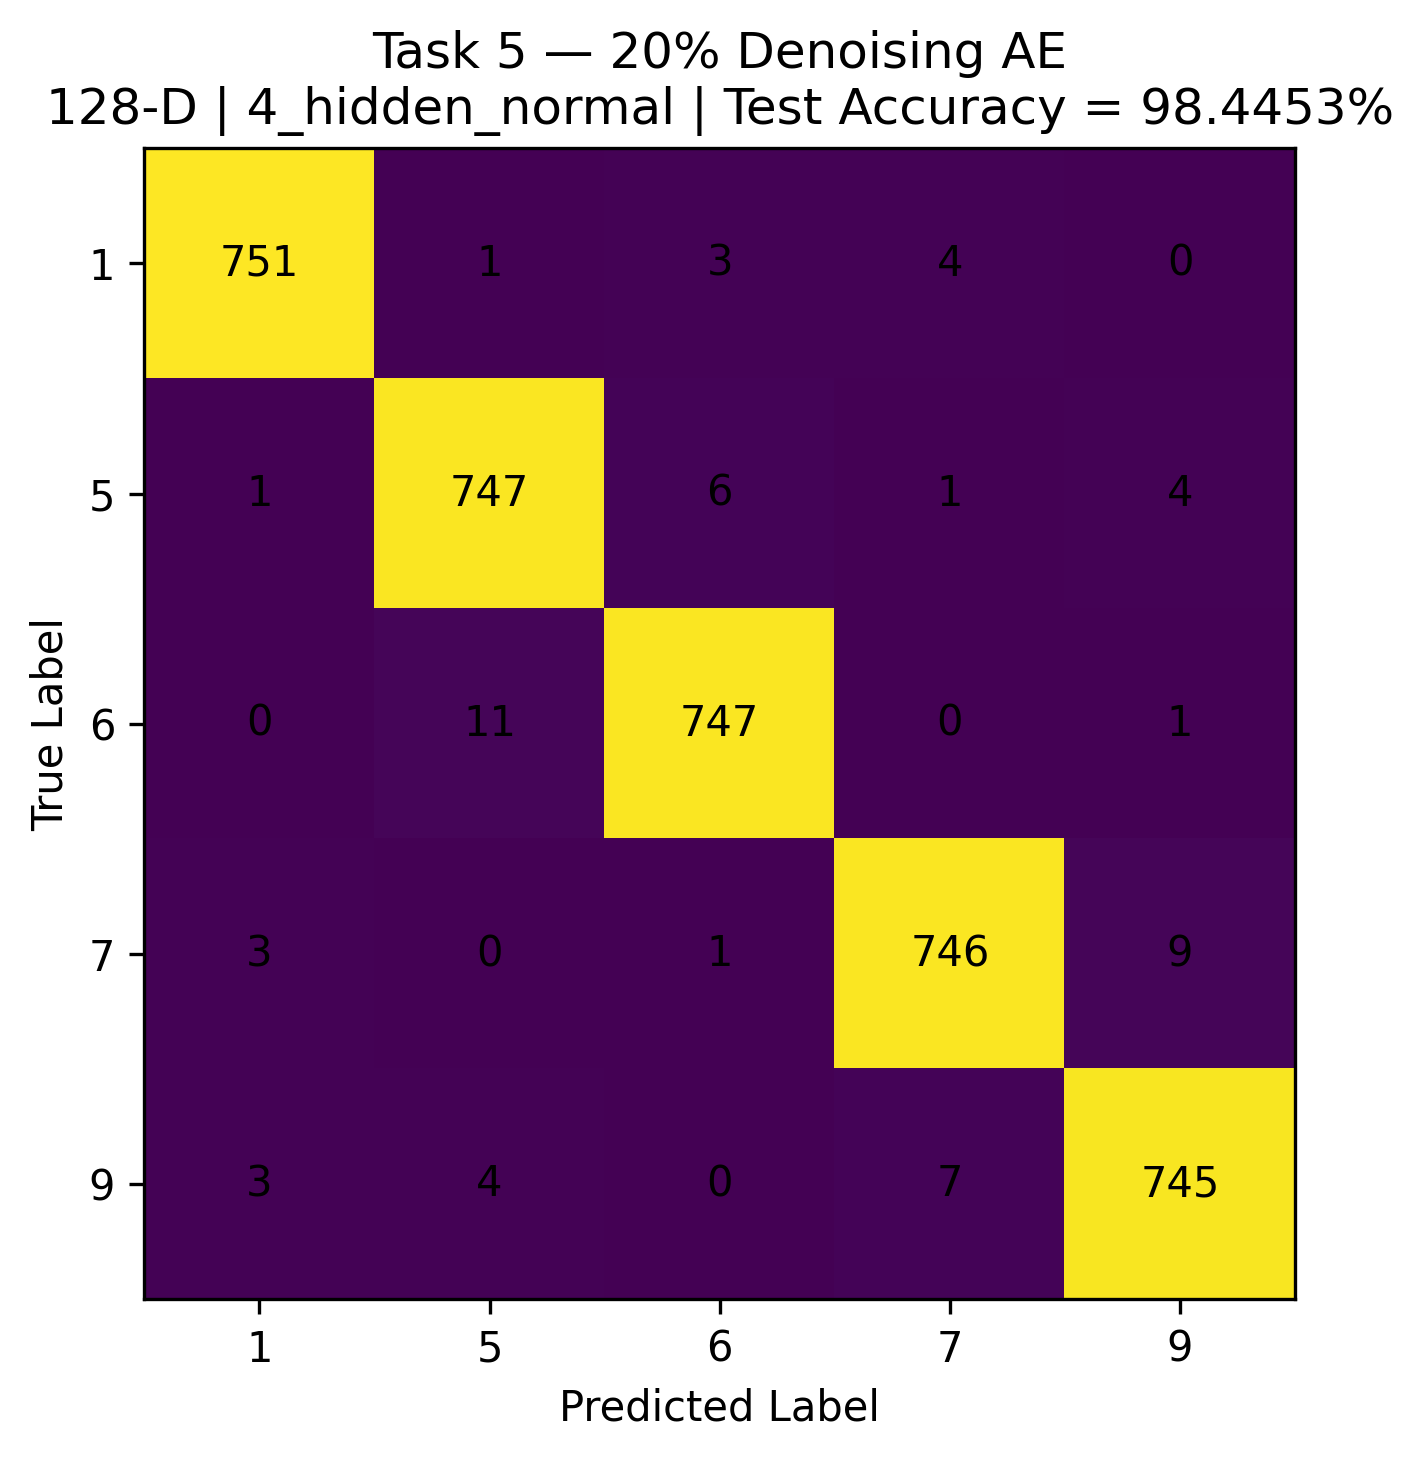
\includegraphics[width=0.88\linewidth,height=0.34\textheight,keepaspectratio]{figures/task5/cnf_img/confusion_matrix_20pct.png}
\caption{Confusion matrix: confusion matrix for 20\% noise.}
\label{fig:task5_1}
\end{figure}

\begin{figure}[H]
\centering
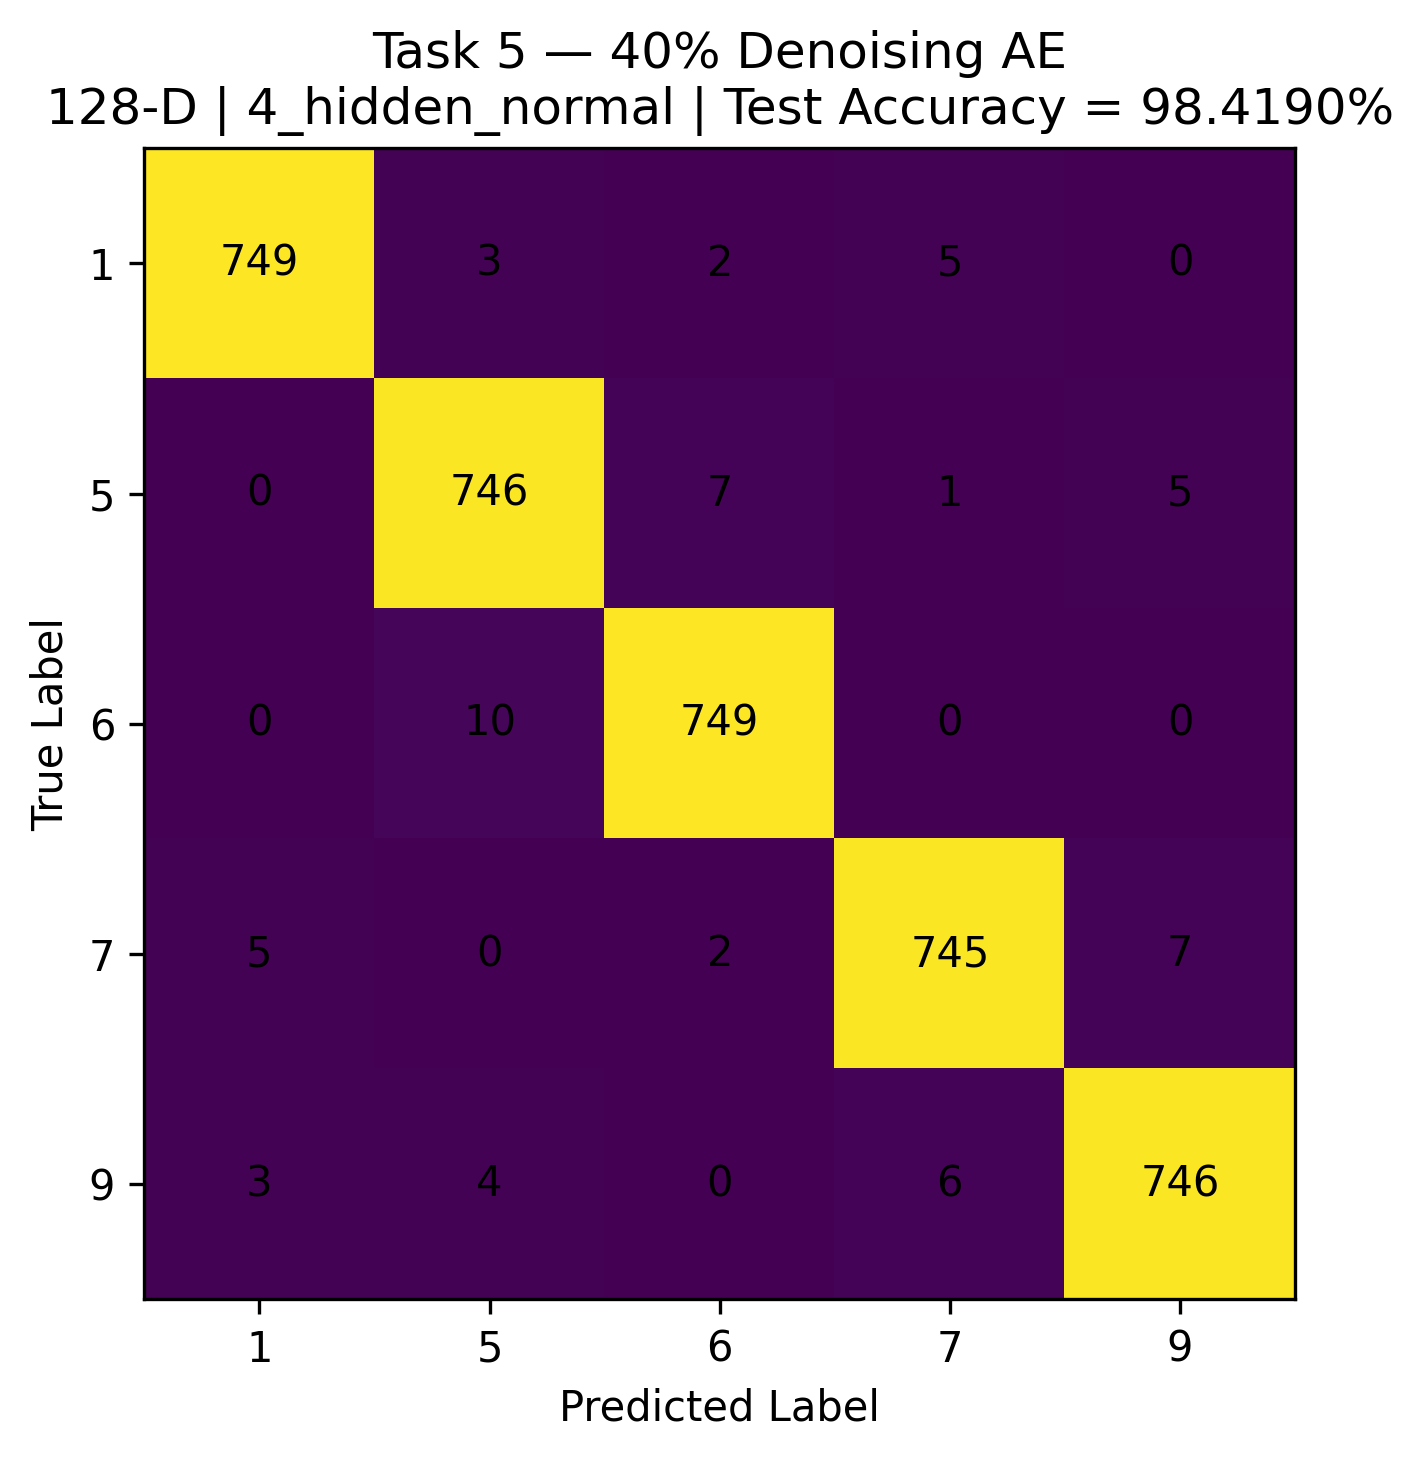
\includegraphics[width=0.88\linewidth,height=0.34\textheight,keepaspectratio]{figures/task5/cnf_img/confusion_matrix_40pct.png}
\caption{Confusion matrix: confusion matrix for 40\% noise.}
\label{fig:task5_2}
\end{figure}

\begin{figure}[H]
\centering
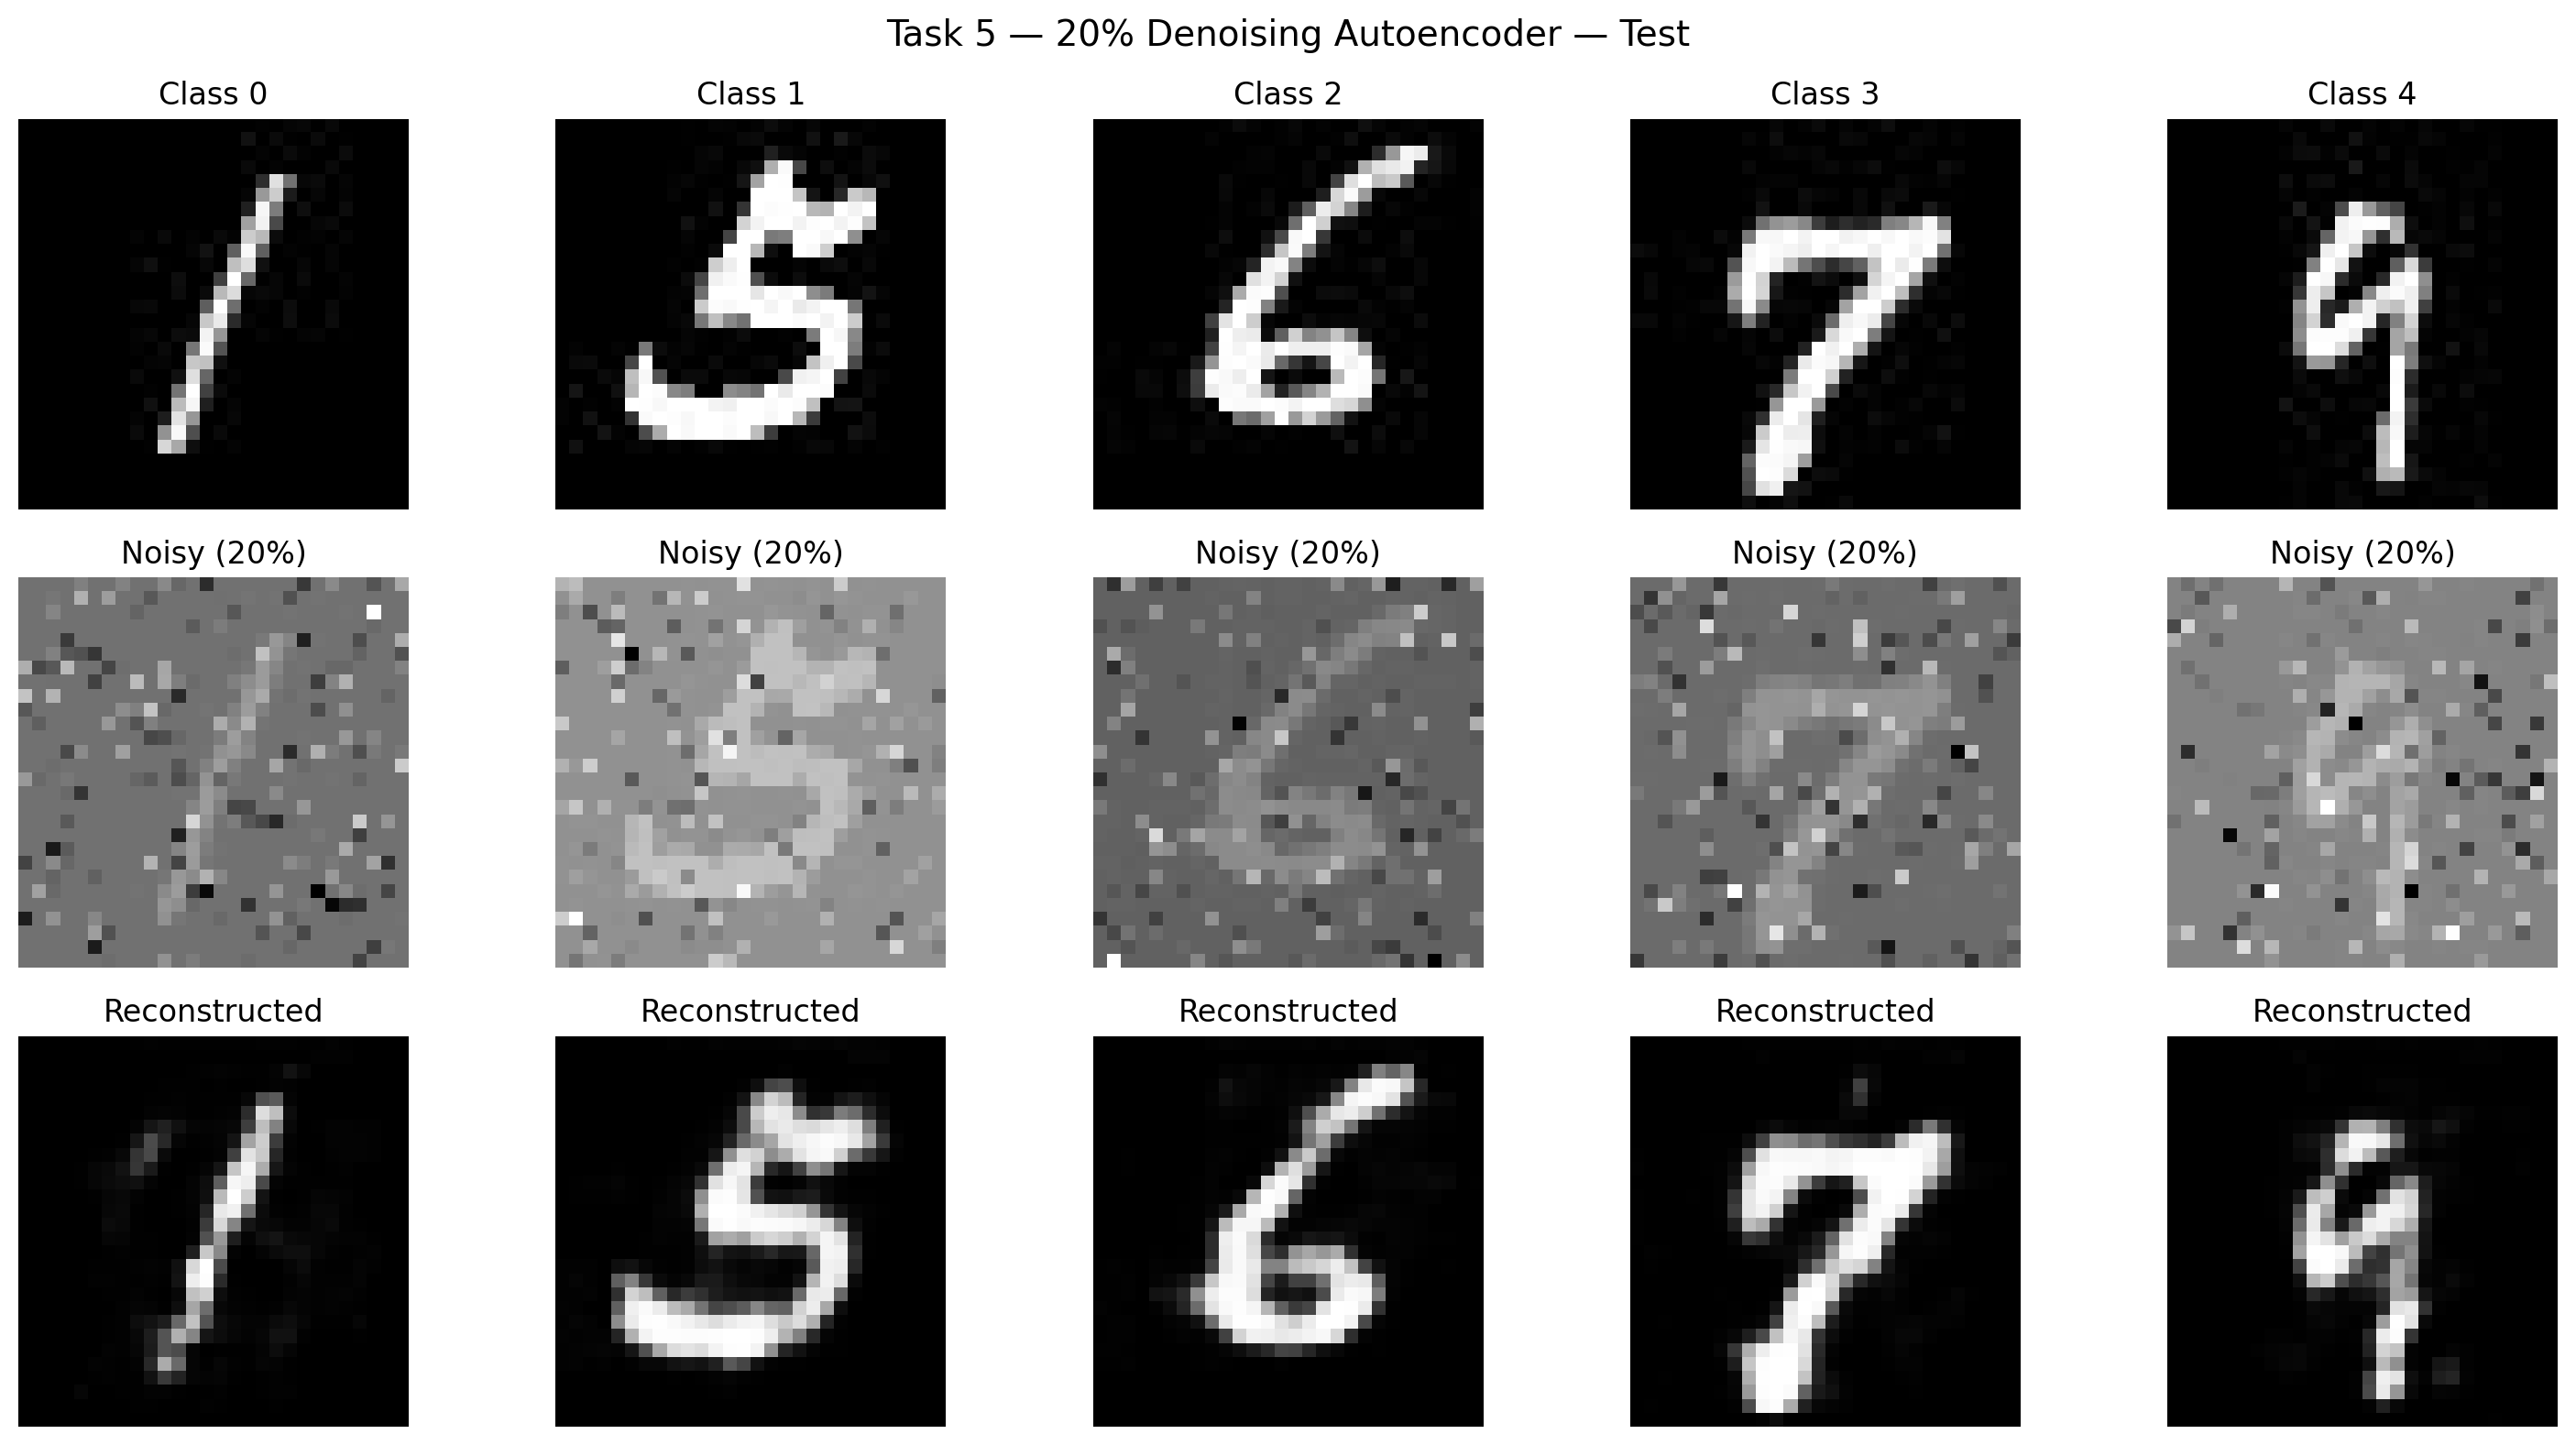
\includegraphics[width=0.88\linewidth,height=0.34\textheight,keepaspectratio]{figures/task5/reconstructions/dae_20pct_test_reconstructions.png}
\caption{Autoencoder reconstruction visualization: dae 20\% noise test reconstructions.}
\label{fig:task5_3}
\end{figure}

\begin{figure}[H]
\centering
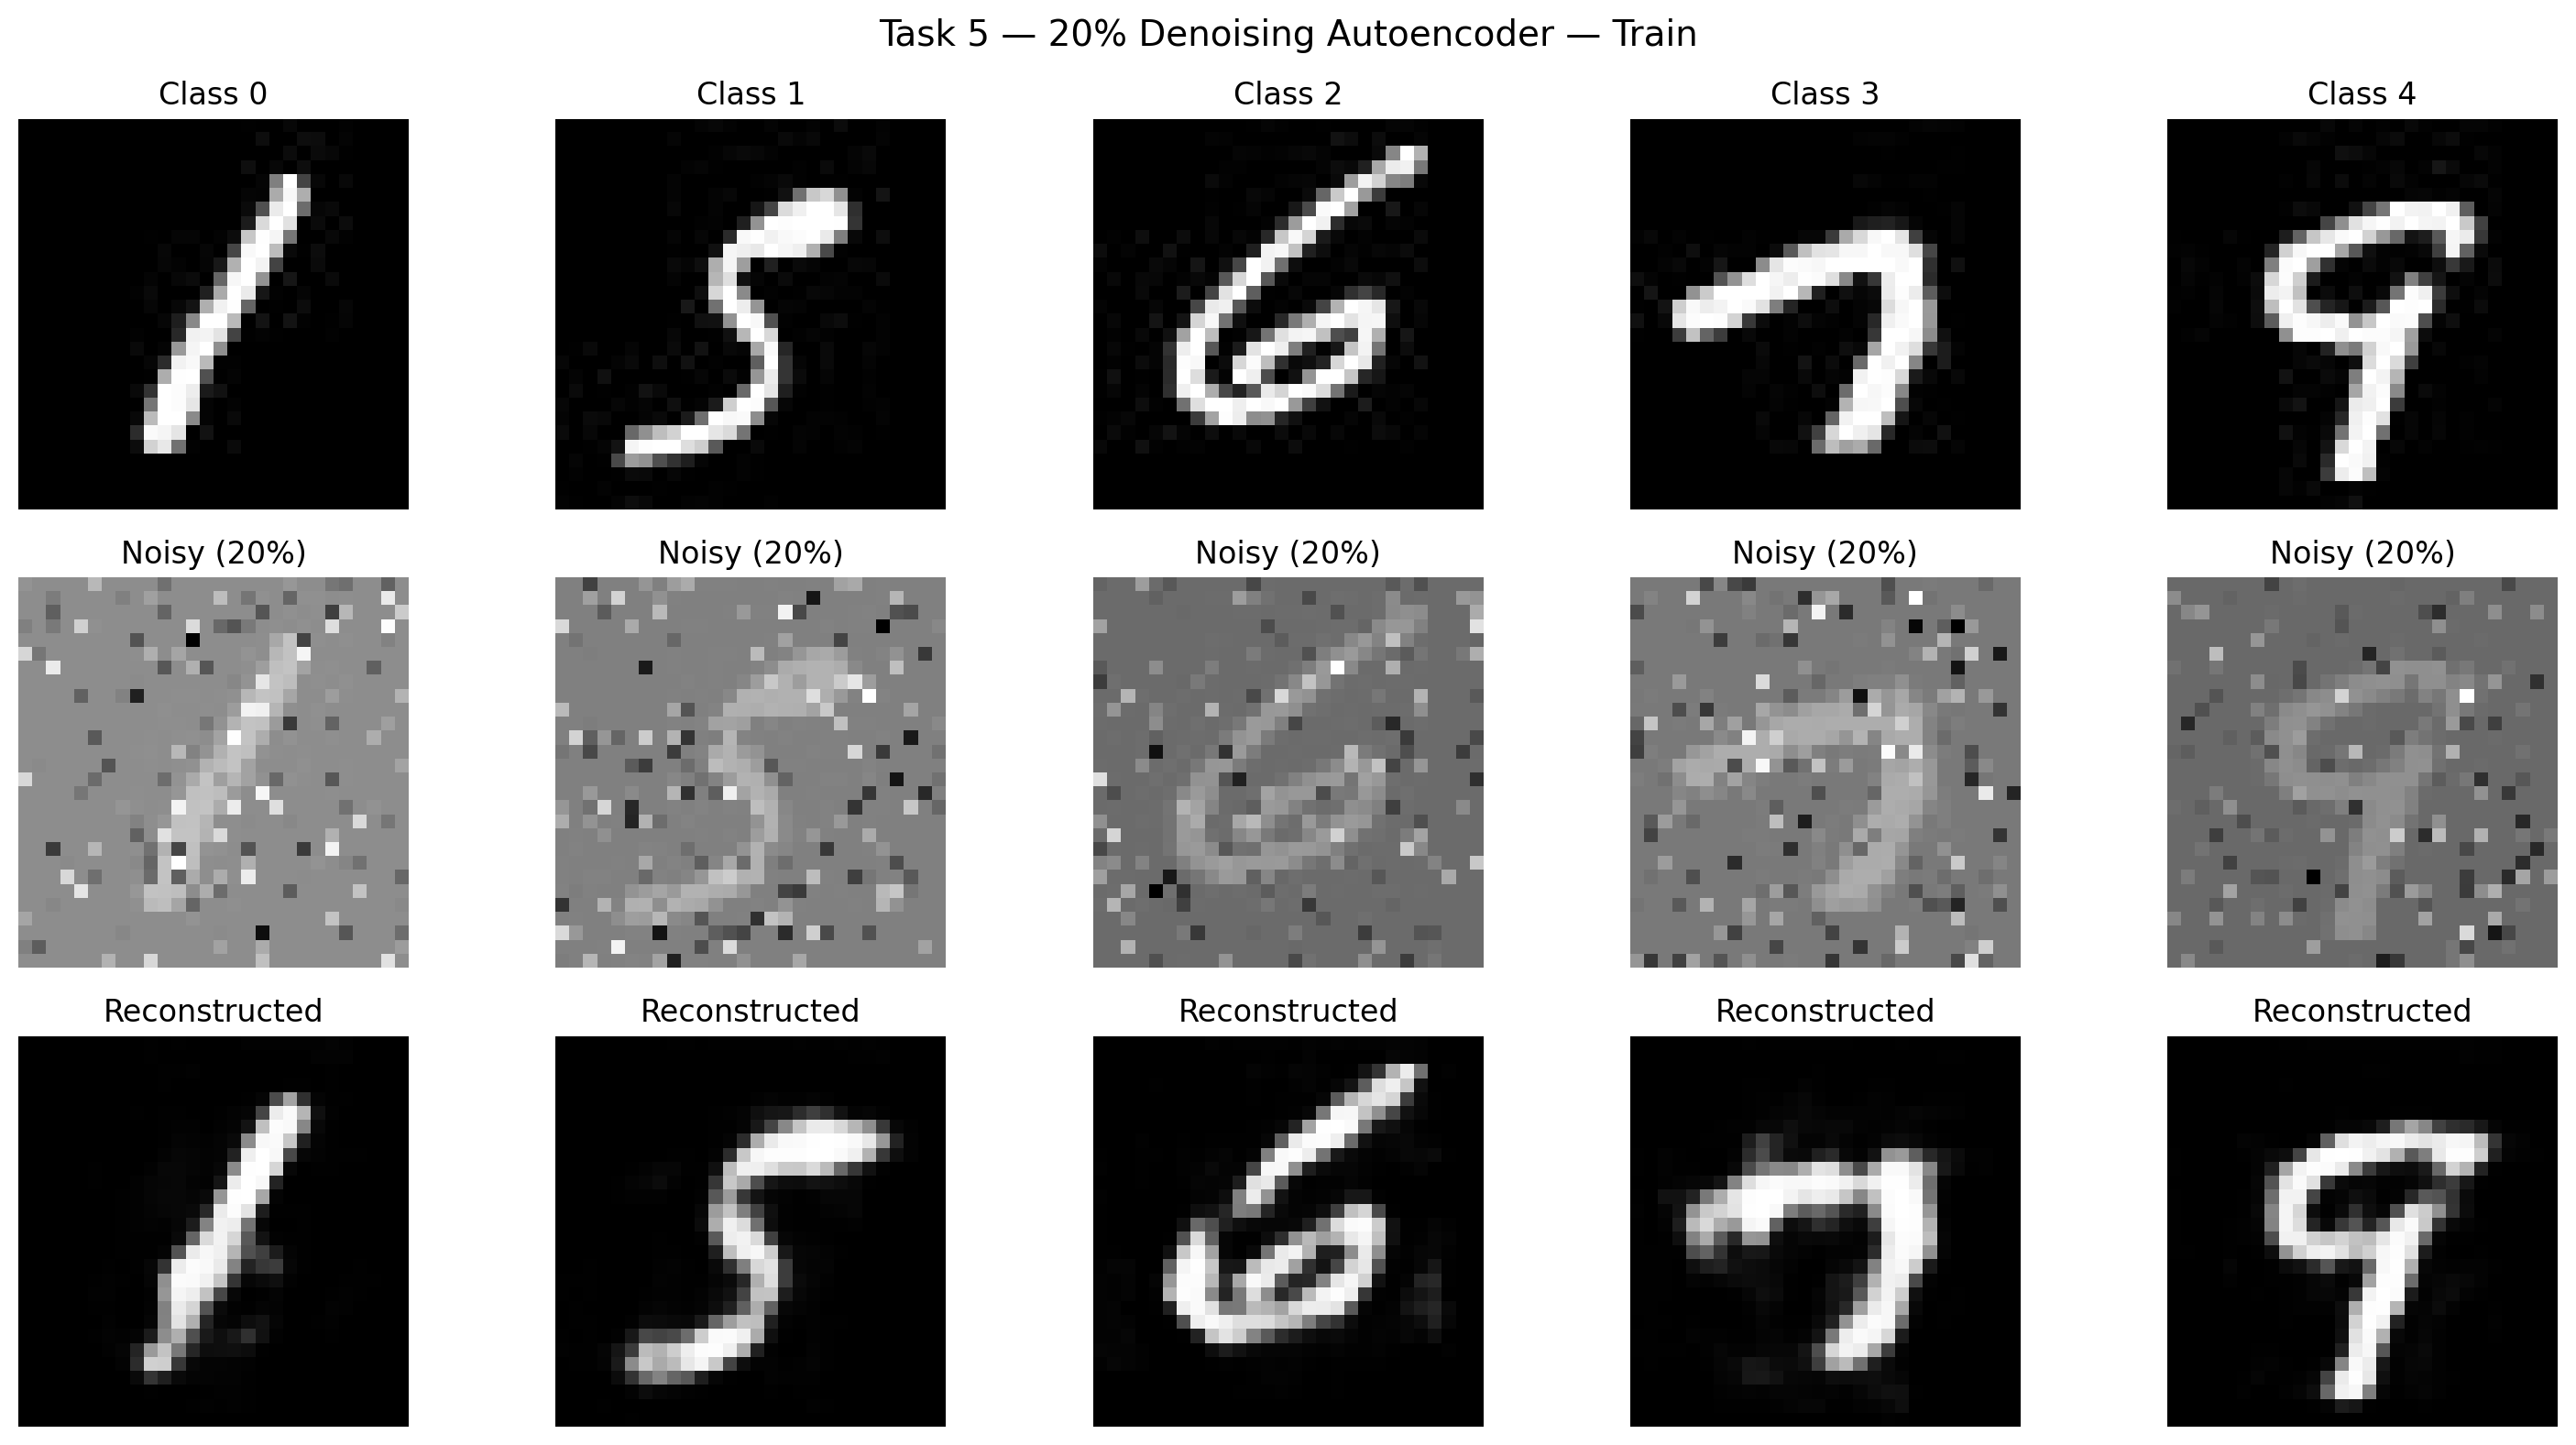
\includegraphics[width=0.88\linewidth,height=0.34\textheight,keepaspectratio]{figures/task5/reconstructions/dae_20pct_train_reconstructions.png}
\caption{Autoencoder reconstruction visualization: dae 20\% noise train reconstructions.}
\label{fig:task5_4}
\end{figure}

\begin{figure}[H]
\centering
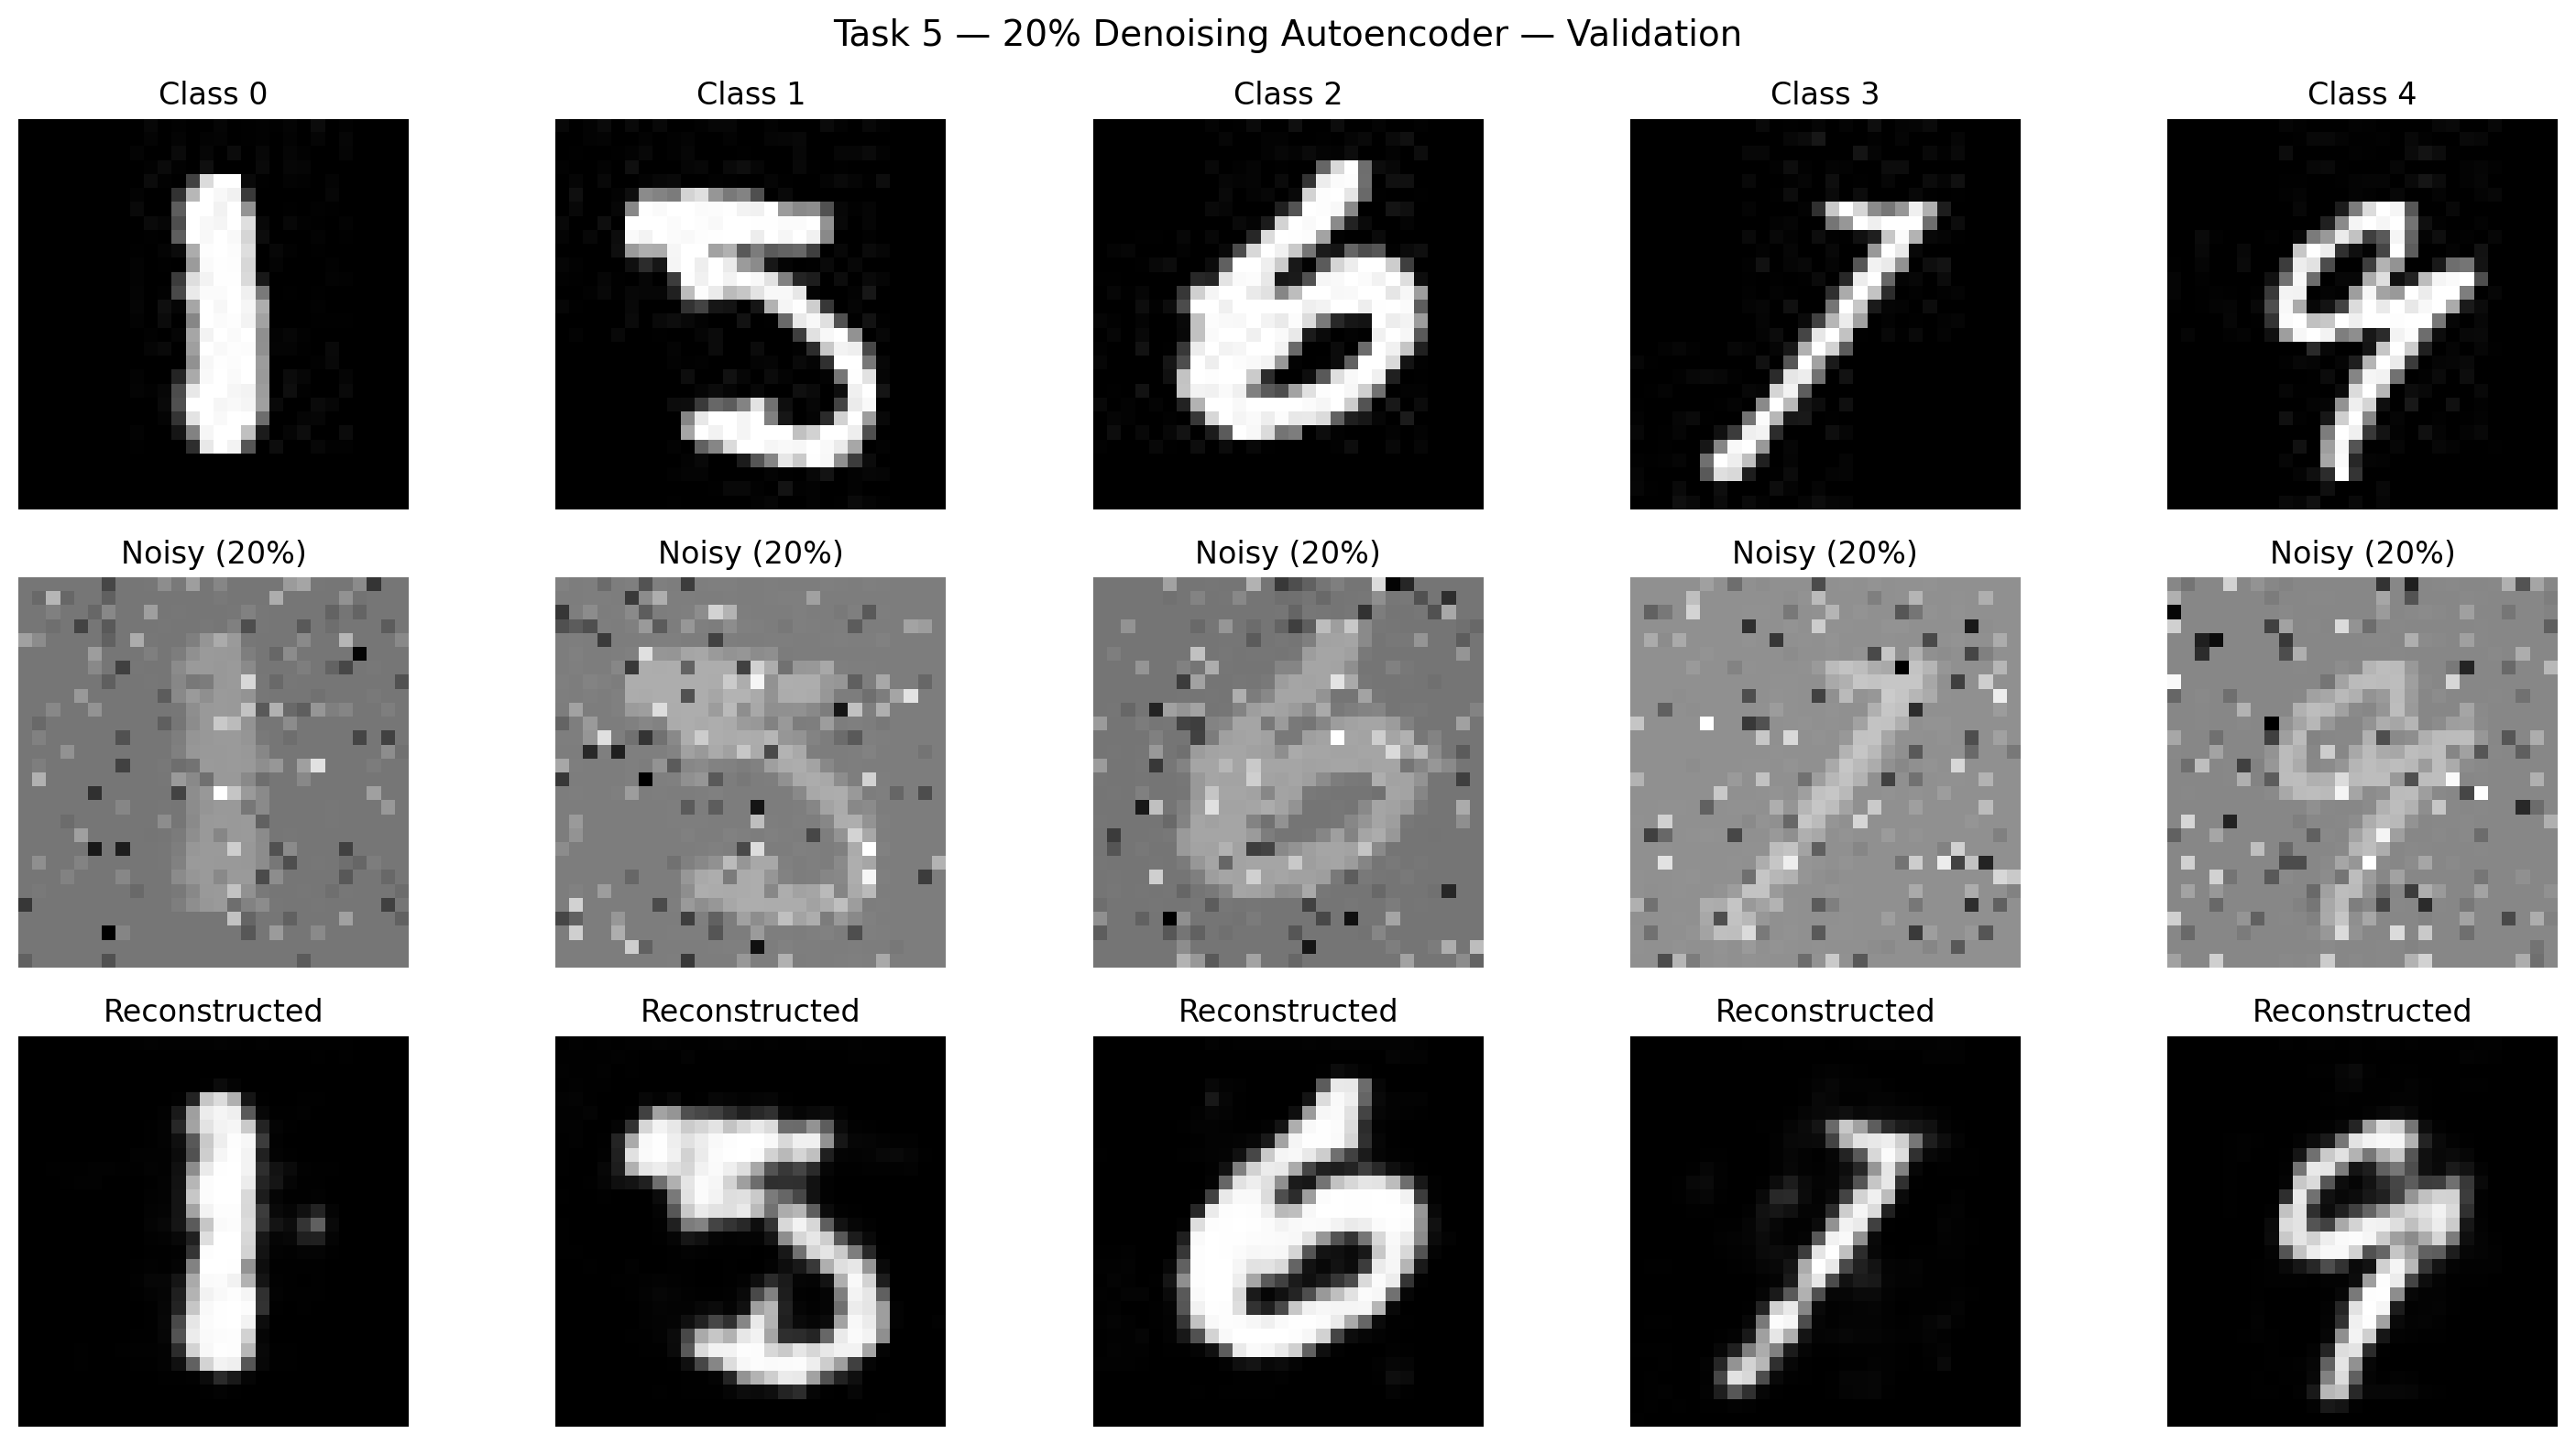
\includegraphics[width=0.88\linewidth,height=0.34\textheight,keepaspectratio]{figures/task5/reconstructions/dae_20pct_validation_reconstructions.png}
\caption{Autoencoder reconstruction visualization: dae 20\% noise validation reconstructions.}
\label{fig:task5_5}
\end{figure}

\begin{figure}[H]
\centering
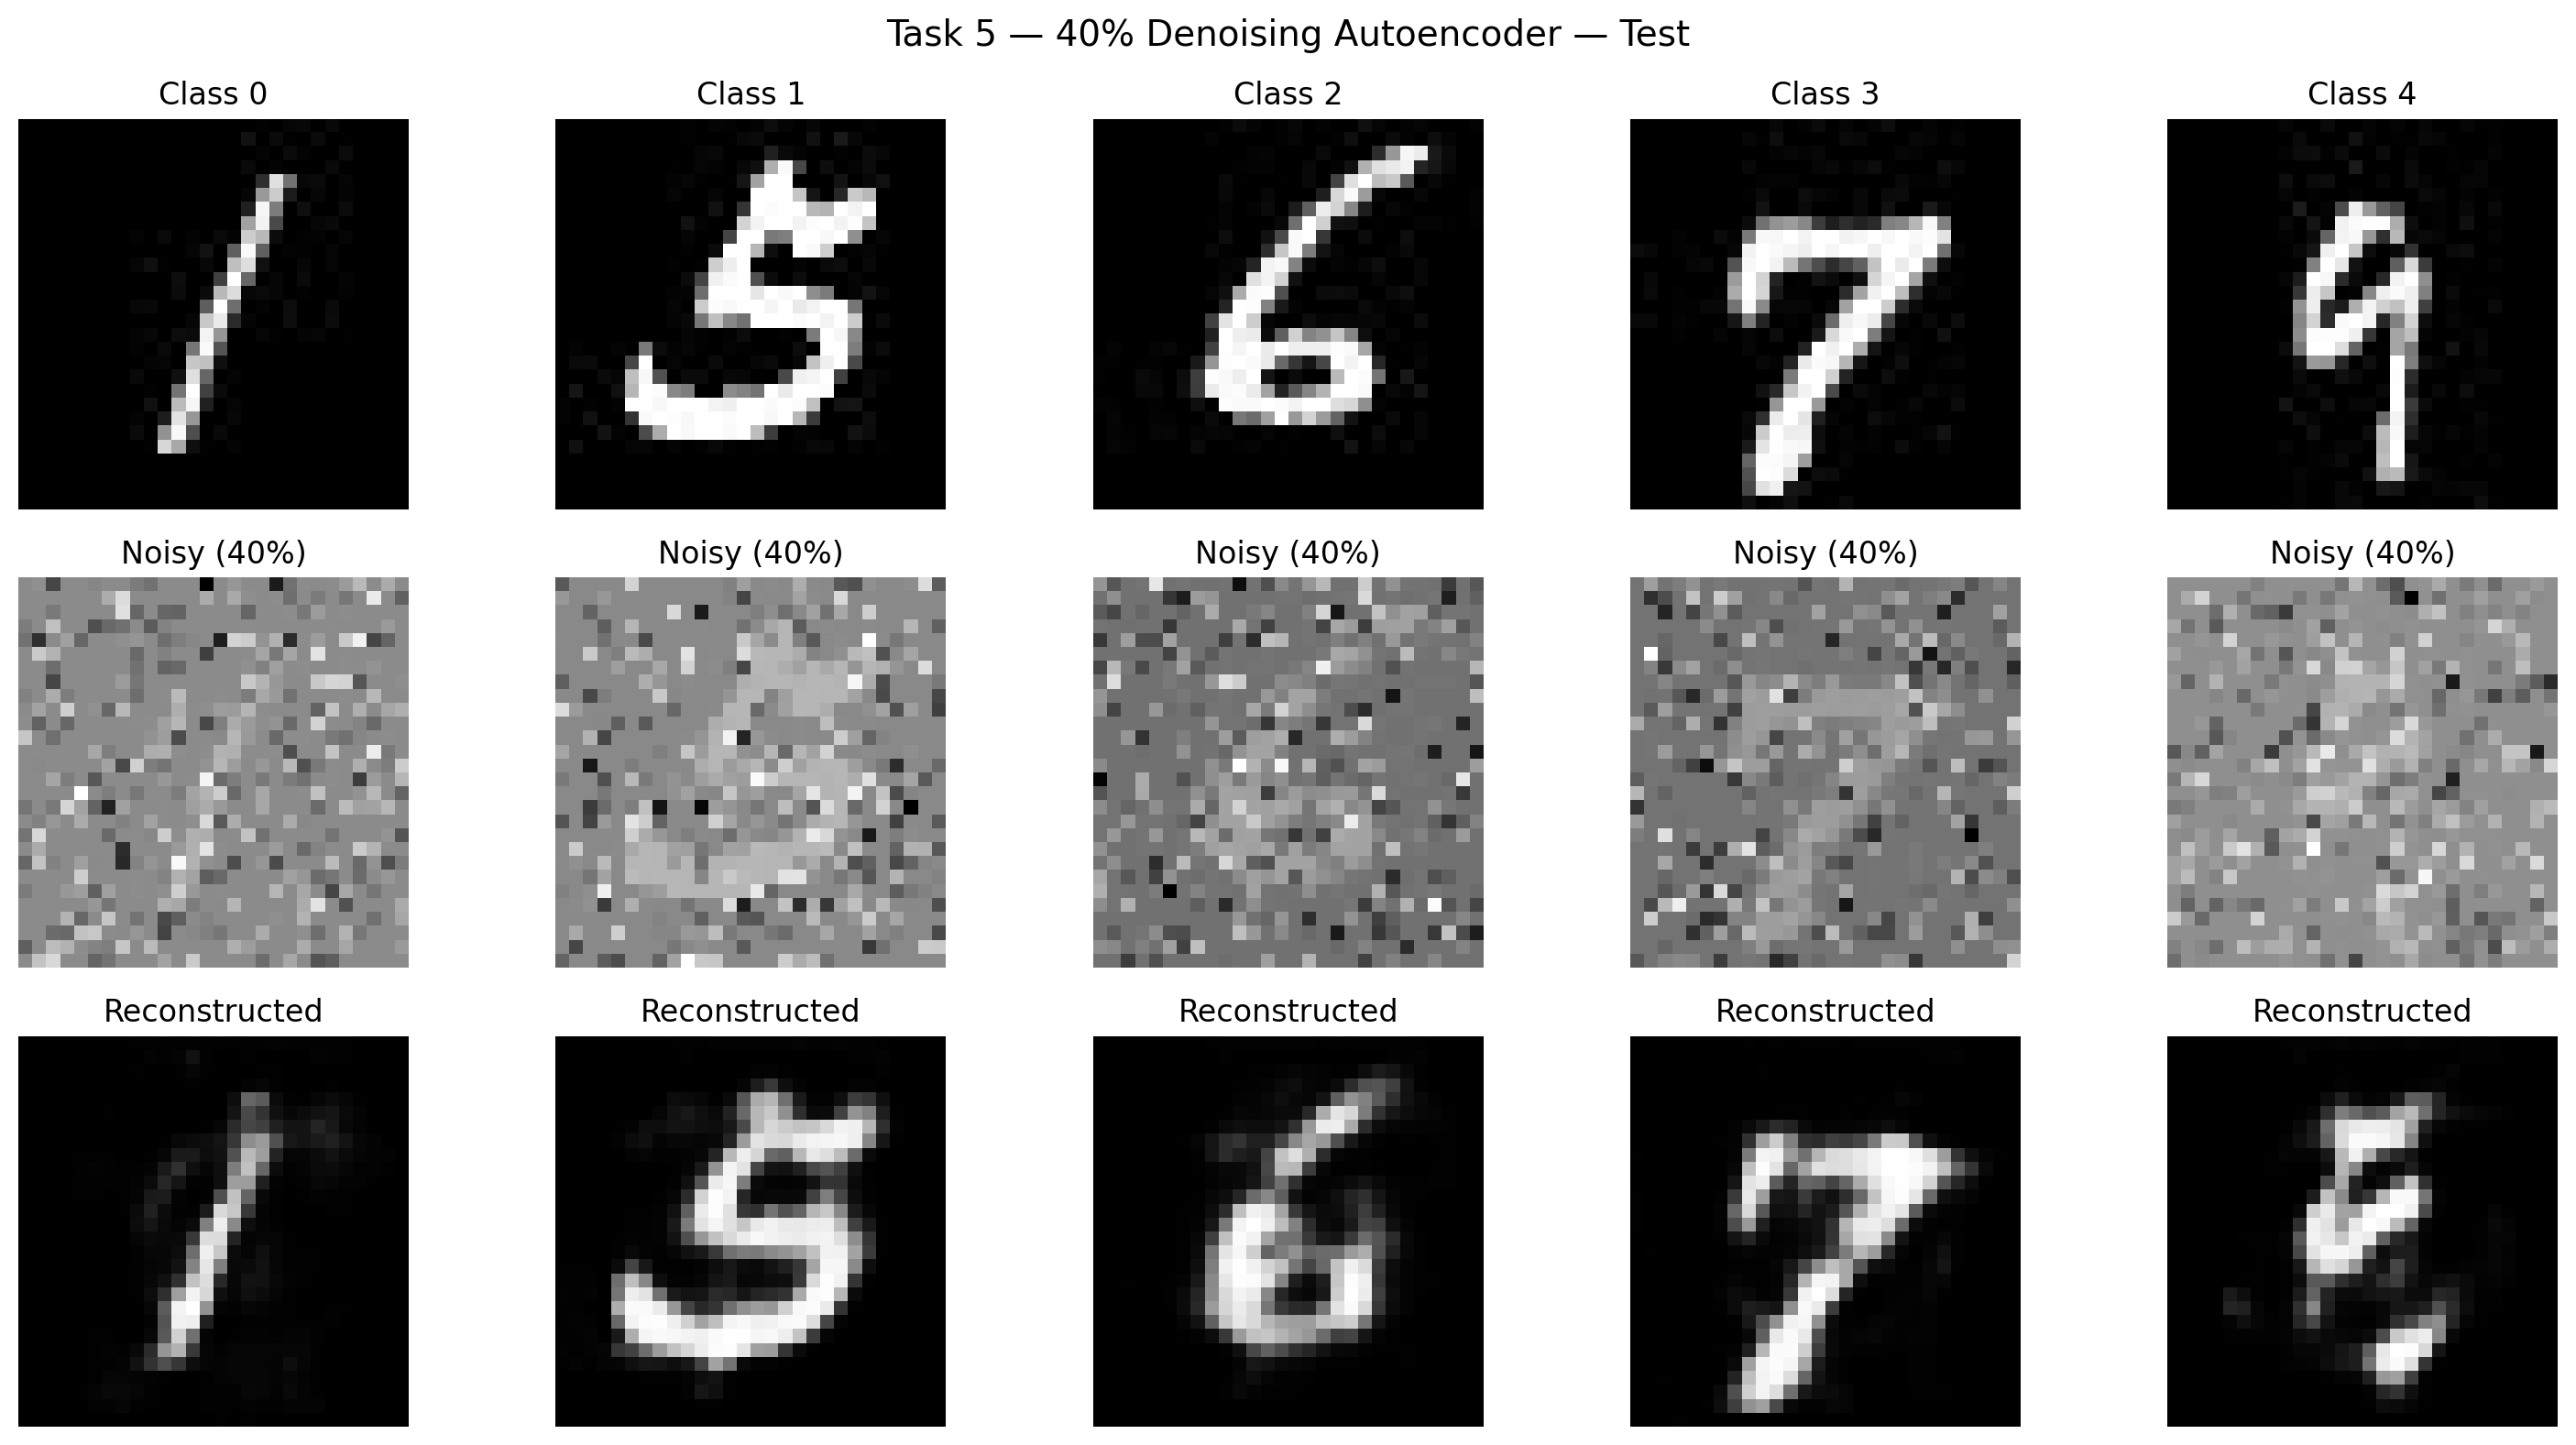
\includegraphics[width=0.88\linewidth,height=0.34\textheight,keepaspectratio]{figures/task5/reconstructions/dae_40pct_test_reconstructions.png}
\caption{Autoencoder reconstruction visualization: dae 40\% noise test reconstructions.}
\label{fig:task5_6}
\end{figure}

\begin{figure}[H]
\centering
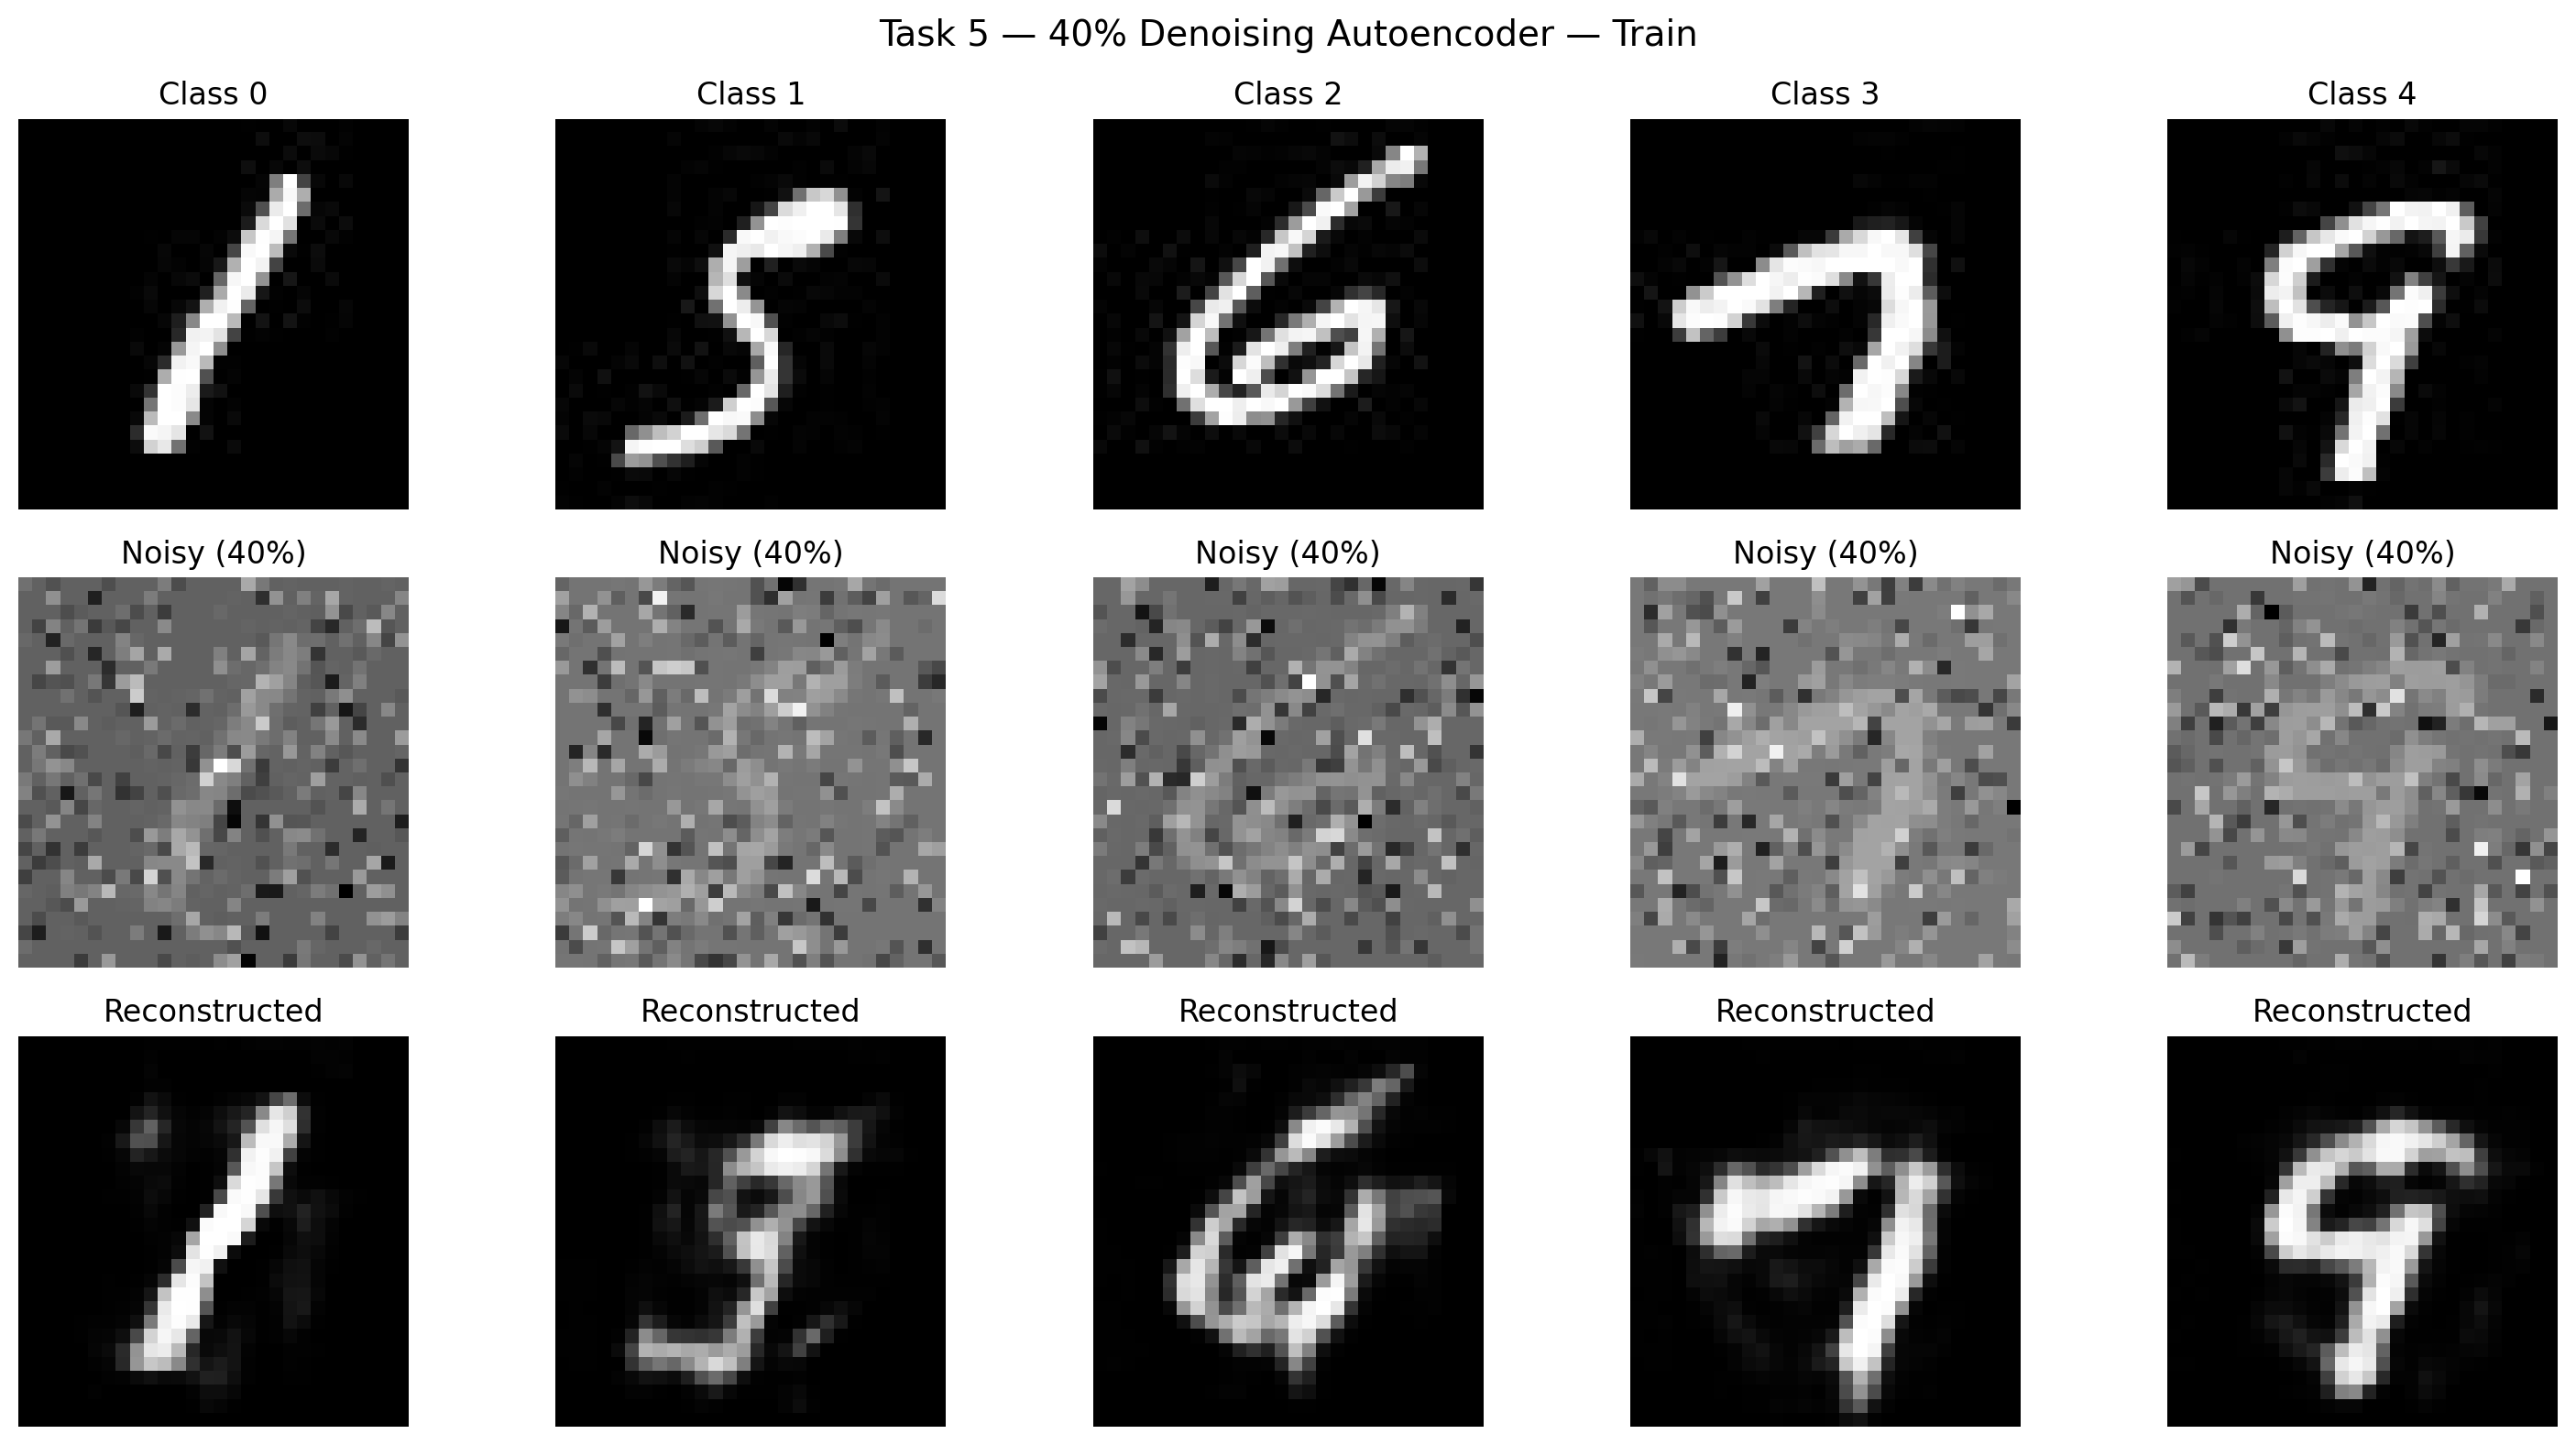
\includegraphics[width=0.88\linewidth,height=0.34\textheight,keepaspectratio]{figures/task5/reconstructions/dae_40pct_train_reconstructions.png}
\caption{Autoencoder reconstruction visualization: dae 40\% noise train reconstructions.}
\label{fig:task5_7}
\end{figure}

\begin{figure}[H]
\centering
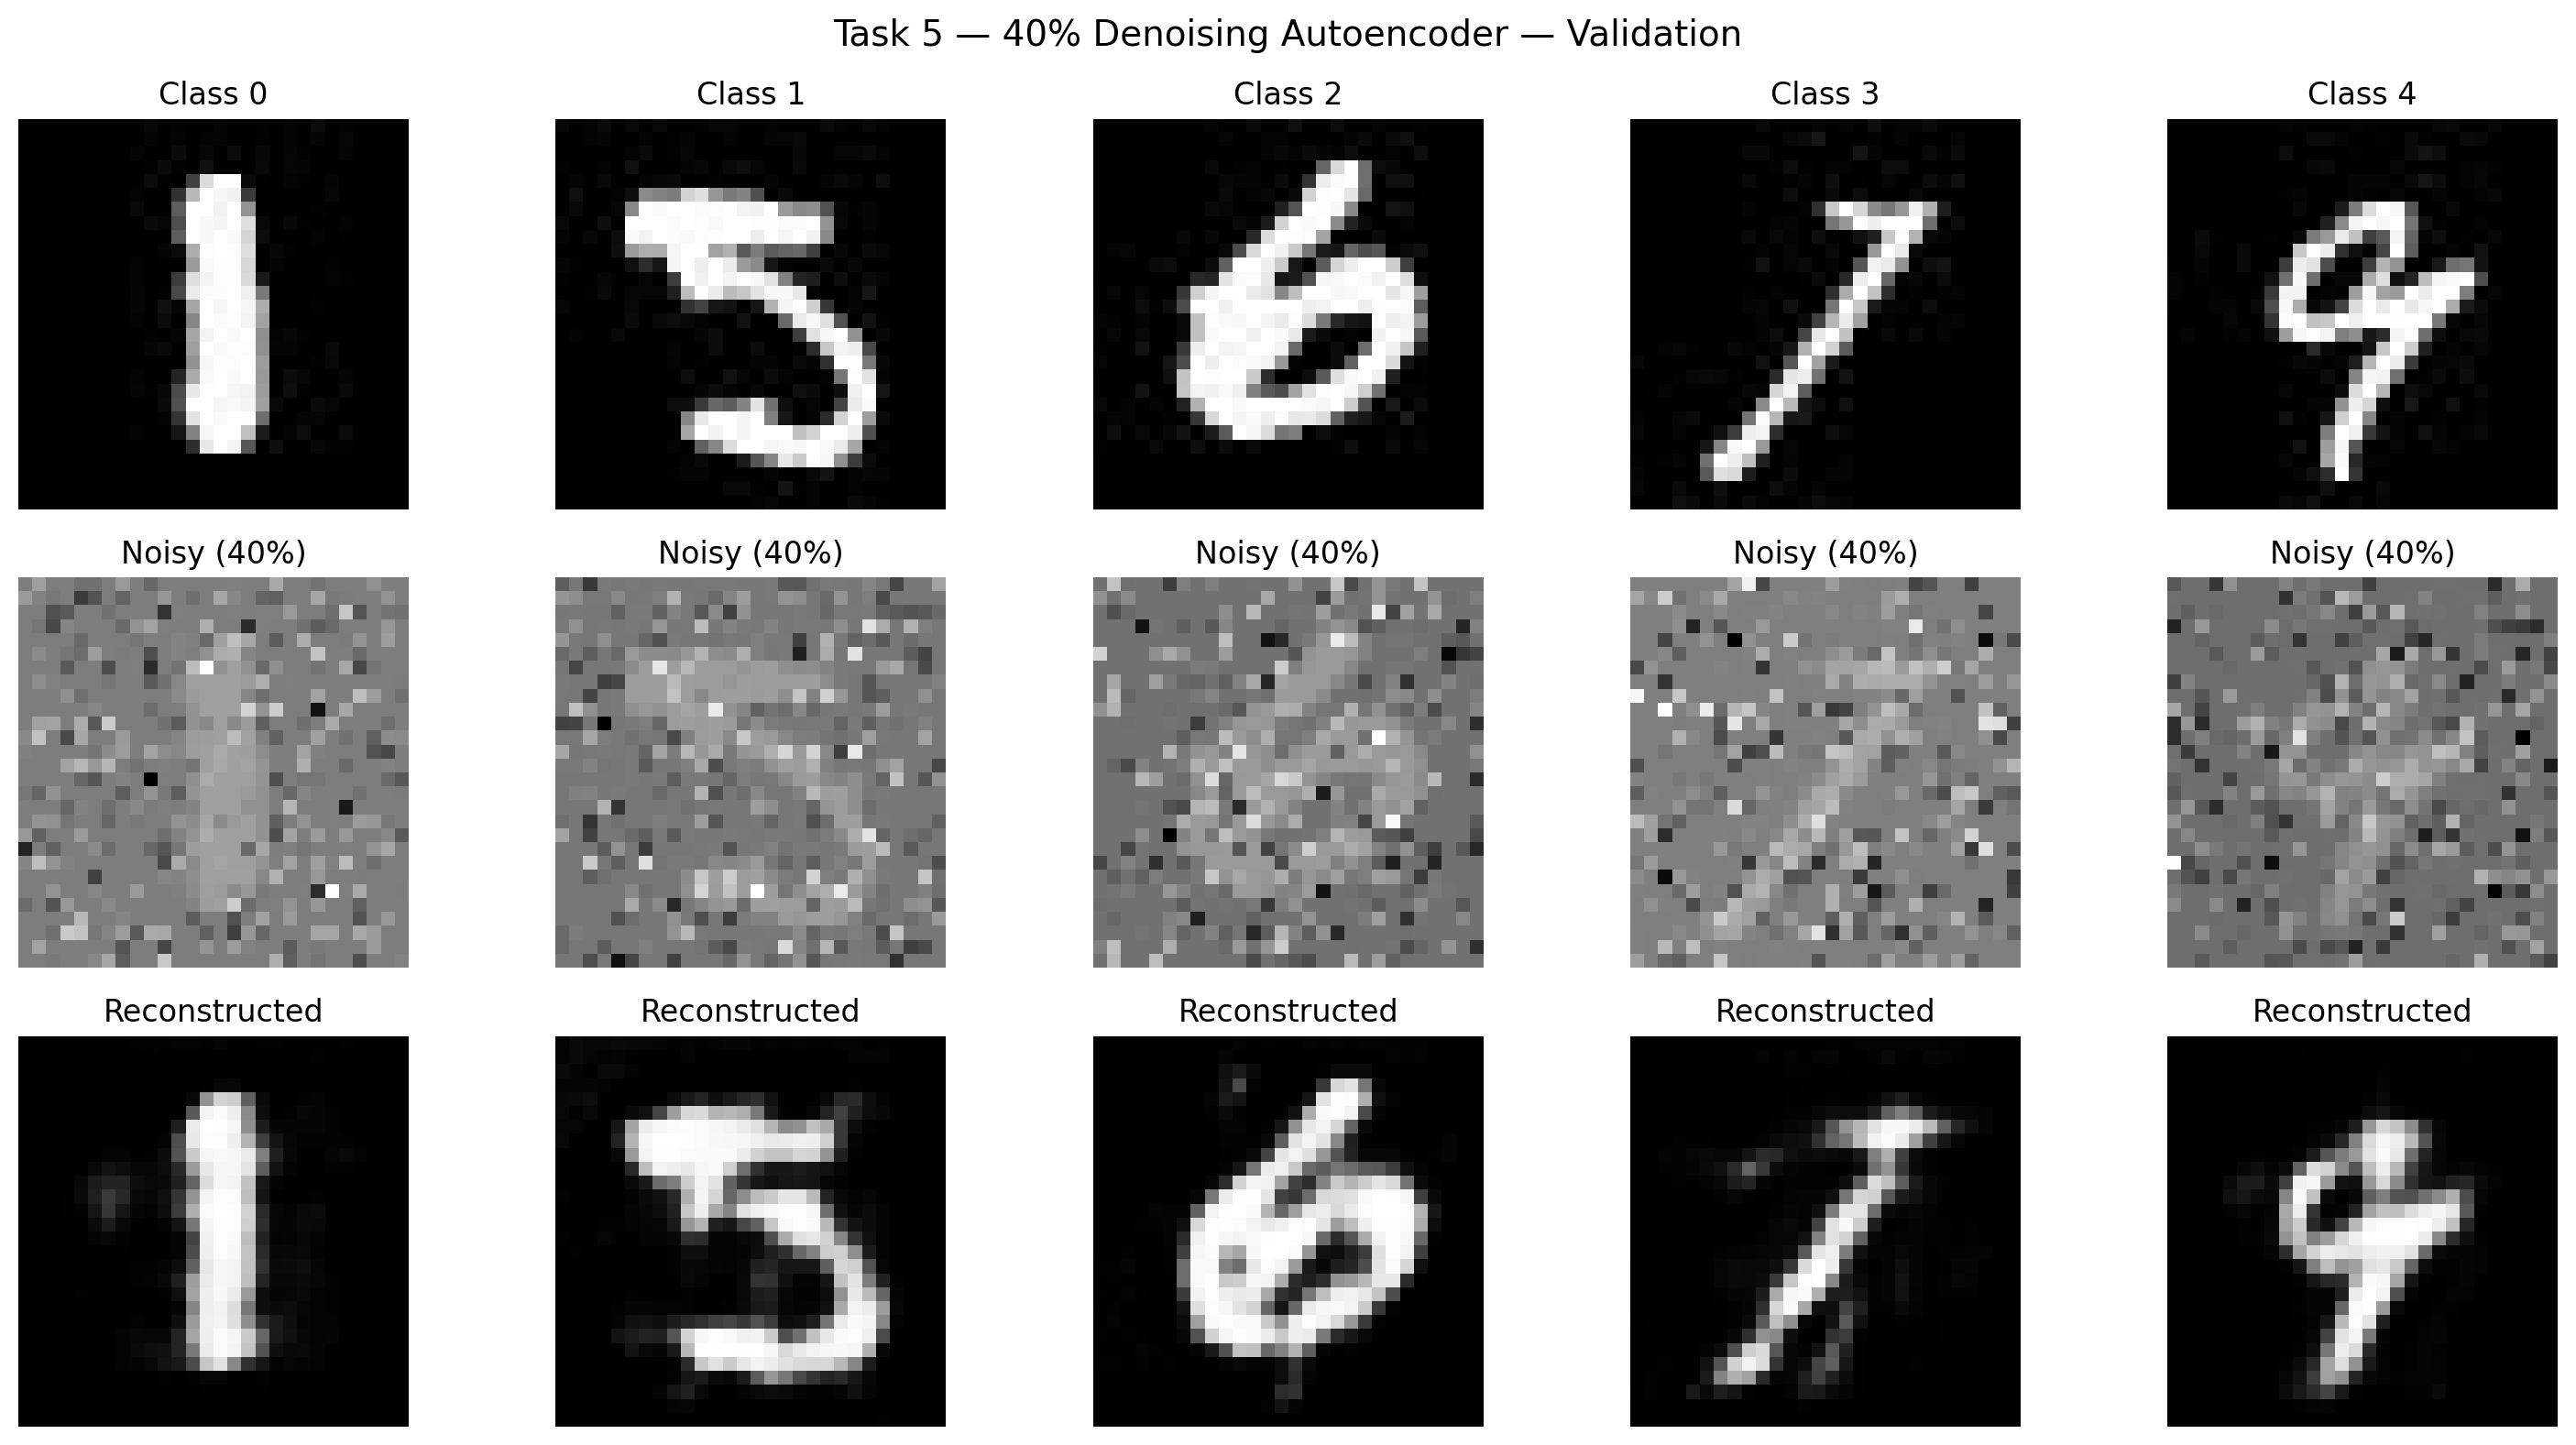
\includegraphics[width=0.88\linewidth,height=0.34\textheight,keepaspectratio]{figures/task5/reconstructions/dae_40pct_validation_reconstructions.png}
\caption{Autoencoder reconstruction visualization: dae 40\% noise validation reconstructions.}
\label{fig:task5_8}
\end{figure}

\FloatBarrier

\section{Task 6: Input-to-Bottleneck Weight Visualization}
\subsection{Method}
For the best 128-dimensional one-hidden-layer autoencoder representation and the two 128-dimensional denoising autoencoders, each bottleneck neuron has 784 incoming weights. Each vector is reshaped into a $28\times28$ map so that the spatial arrangement corresponds to the original image coordinates. The color map encodes signed weight values; the weights themselves are not modified by the visualization. Eight pages of 16 neurons are provided for each model, giving 24 figures in total.

\subsection{Interpretation}
The weight maps are diagnostic visualizations of learned connections, not reconstructed digit examples. Positive and negative colors indicate the sign of the weights, while spatial patterns show which input locations have stronger connections to each bottleneck unit. A comparison should focus on differences in spatial organization and contrast across the conventional AE and the two DAEs; these maps alone do not establish semantic meaning for a neuron.

% Automatically generated figure inventory for task6.

\begin{figure}[H]
\centering
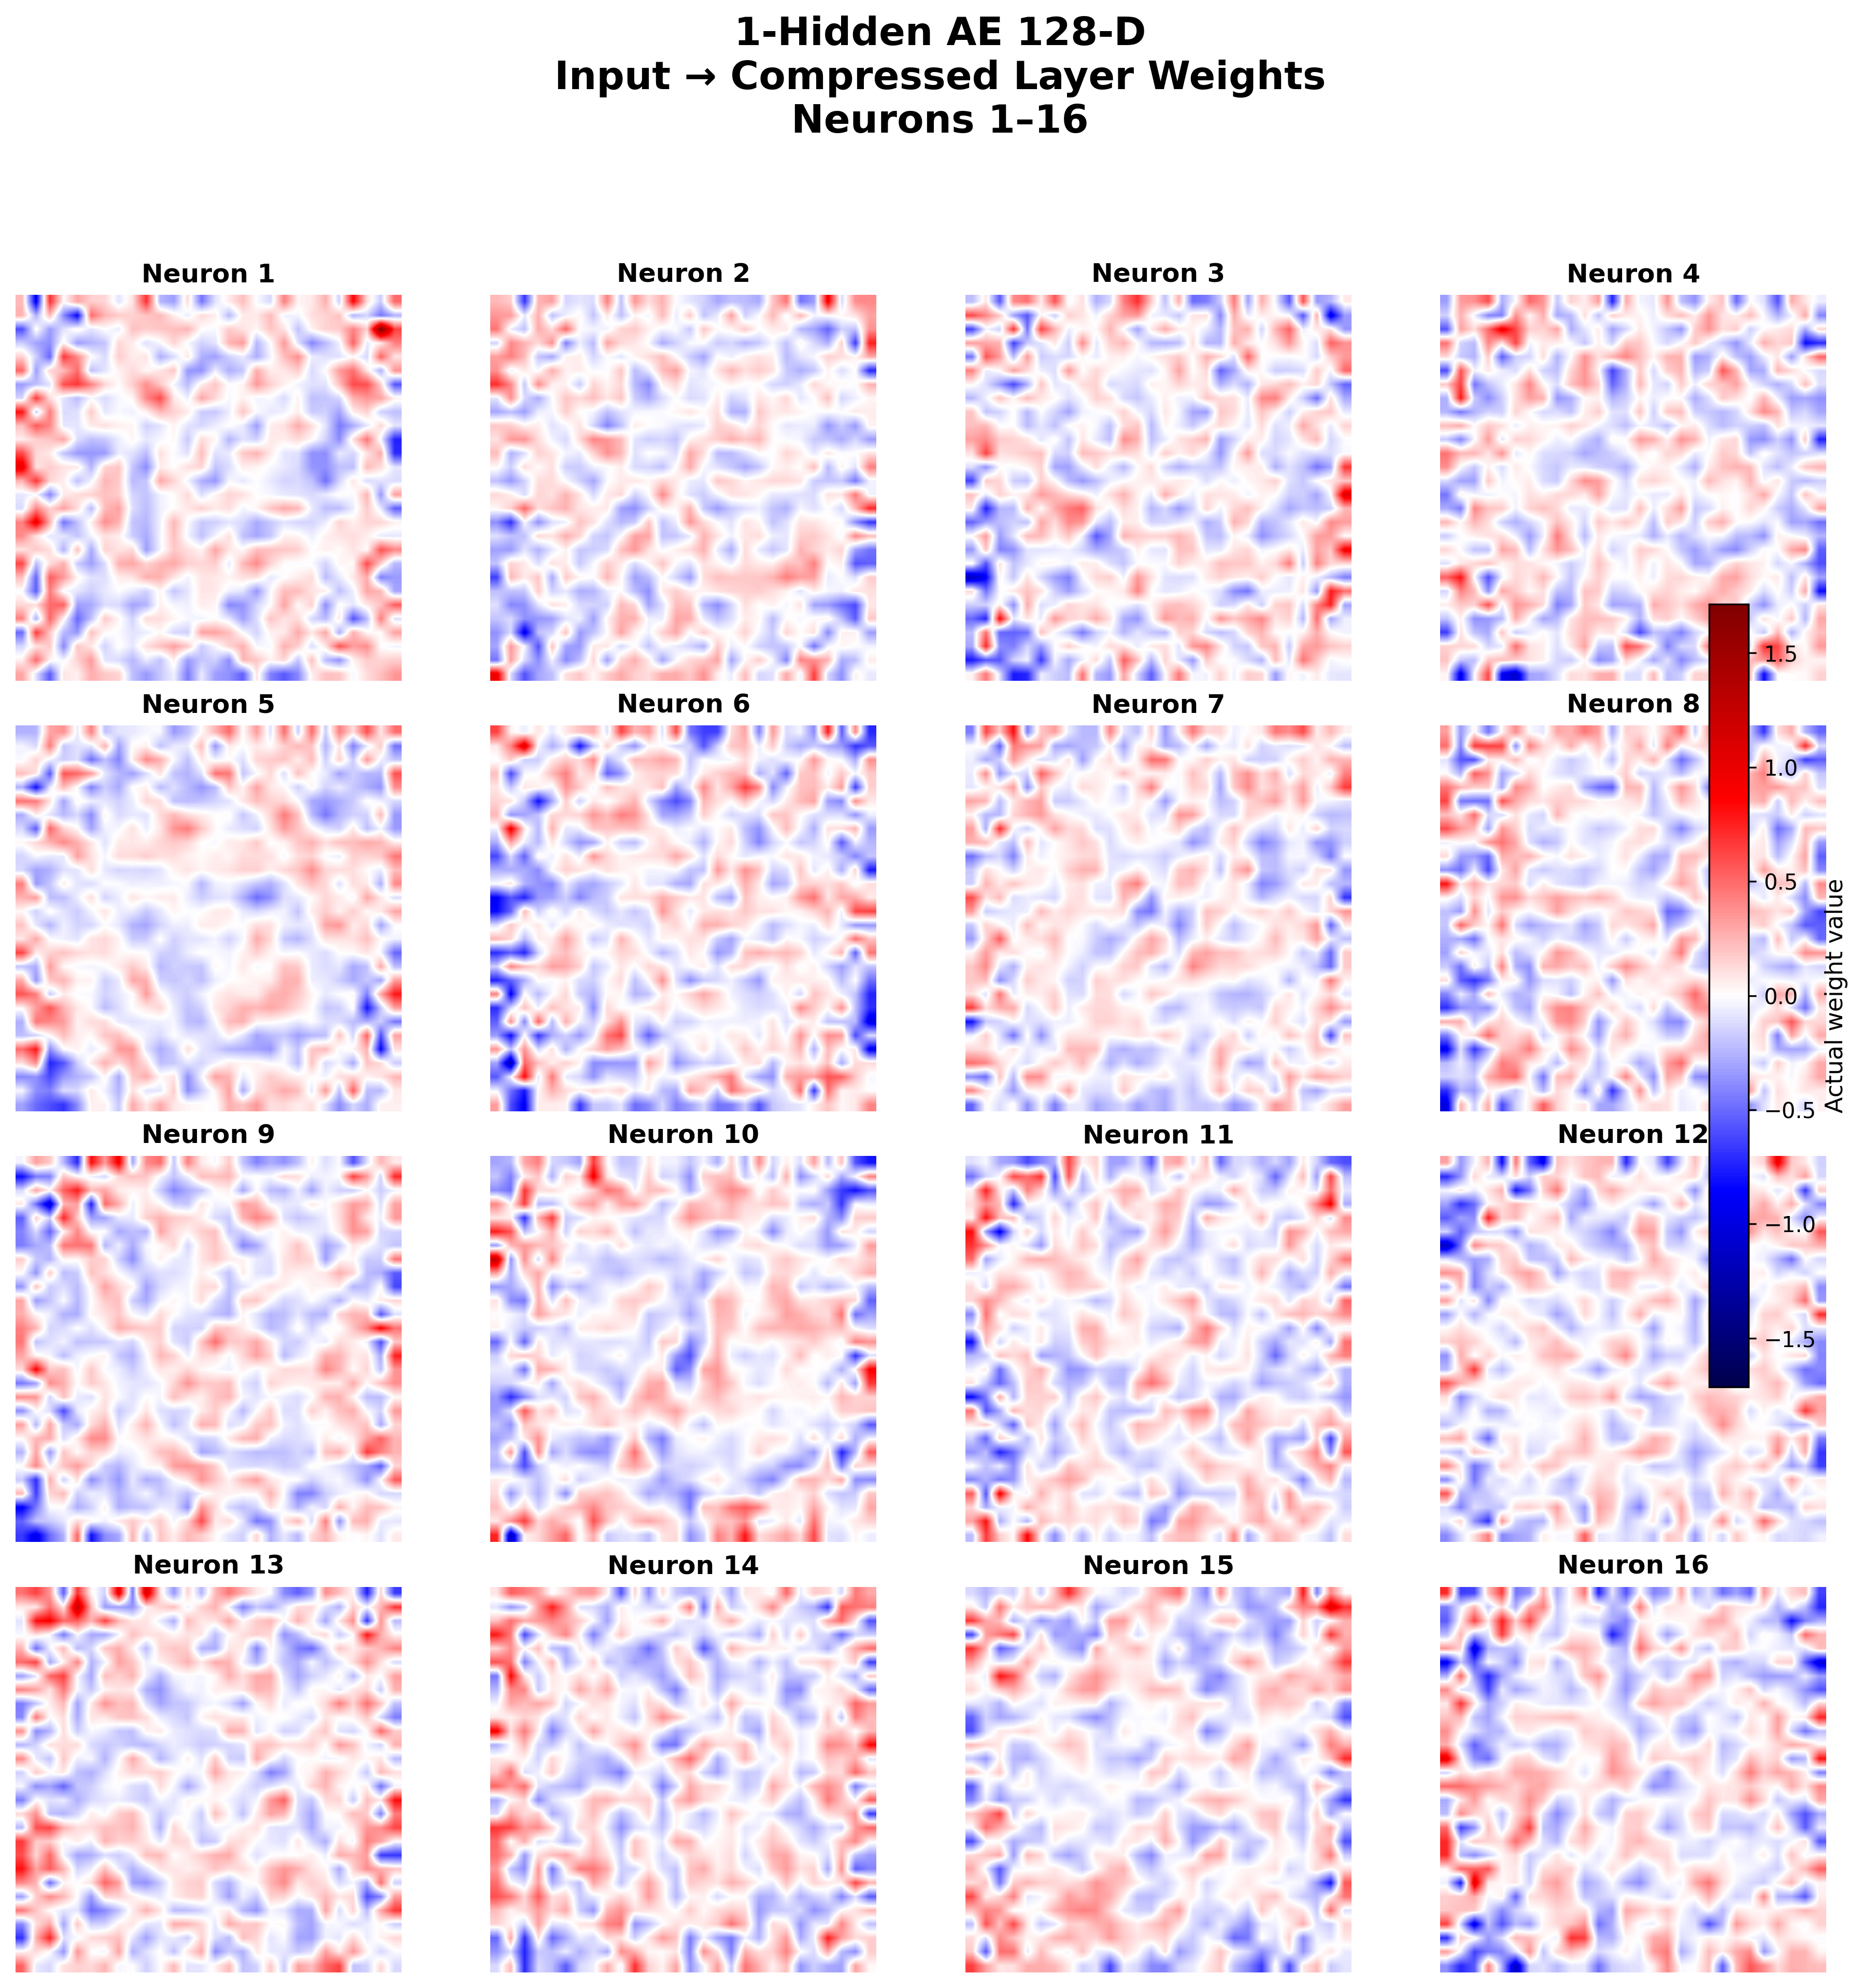
\includegraphics[width=0.99\linewidth,height=0.72\textheight,keepaspectratio]{figures/task6/1_hidden_ae/neurons_001_016.png}
\caption{Input-to-bottleneck weight visualization for neurons 1--16.}
\label{fig:task6_1}
\end{figure}

\begin{figure}[H]
\centering
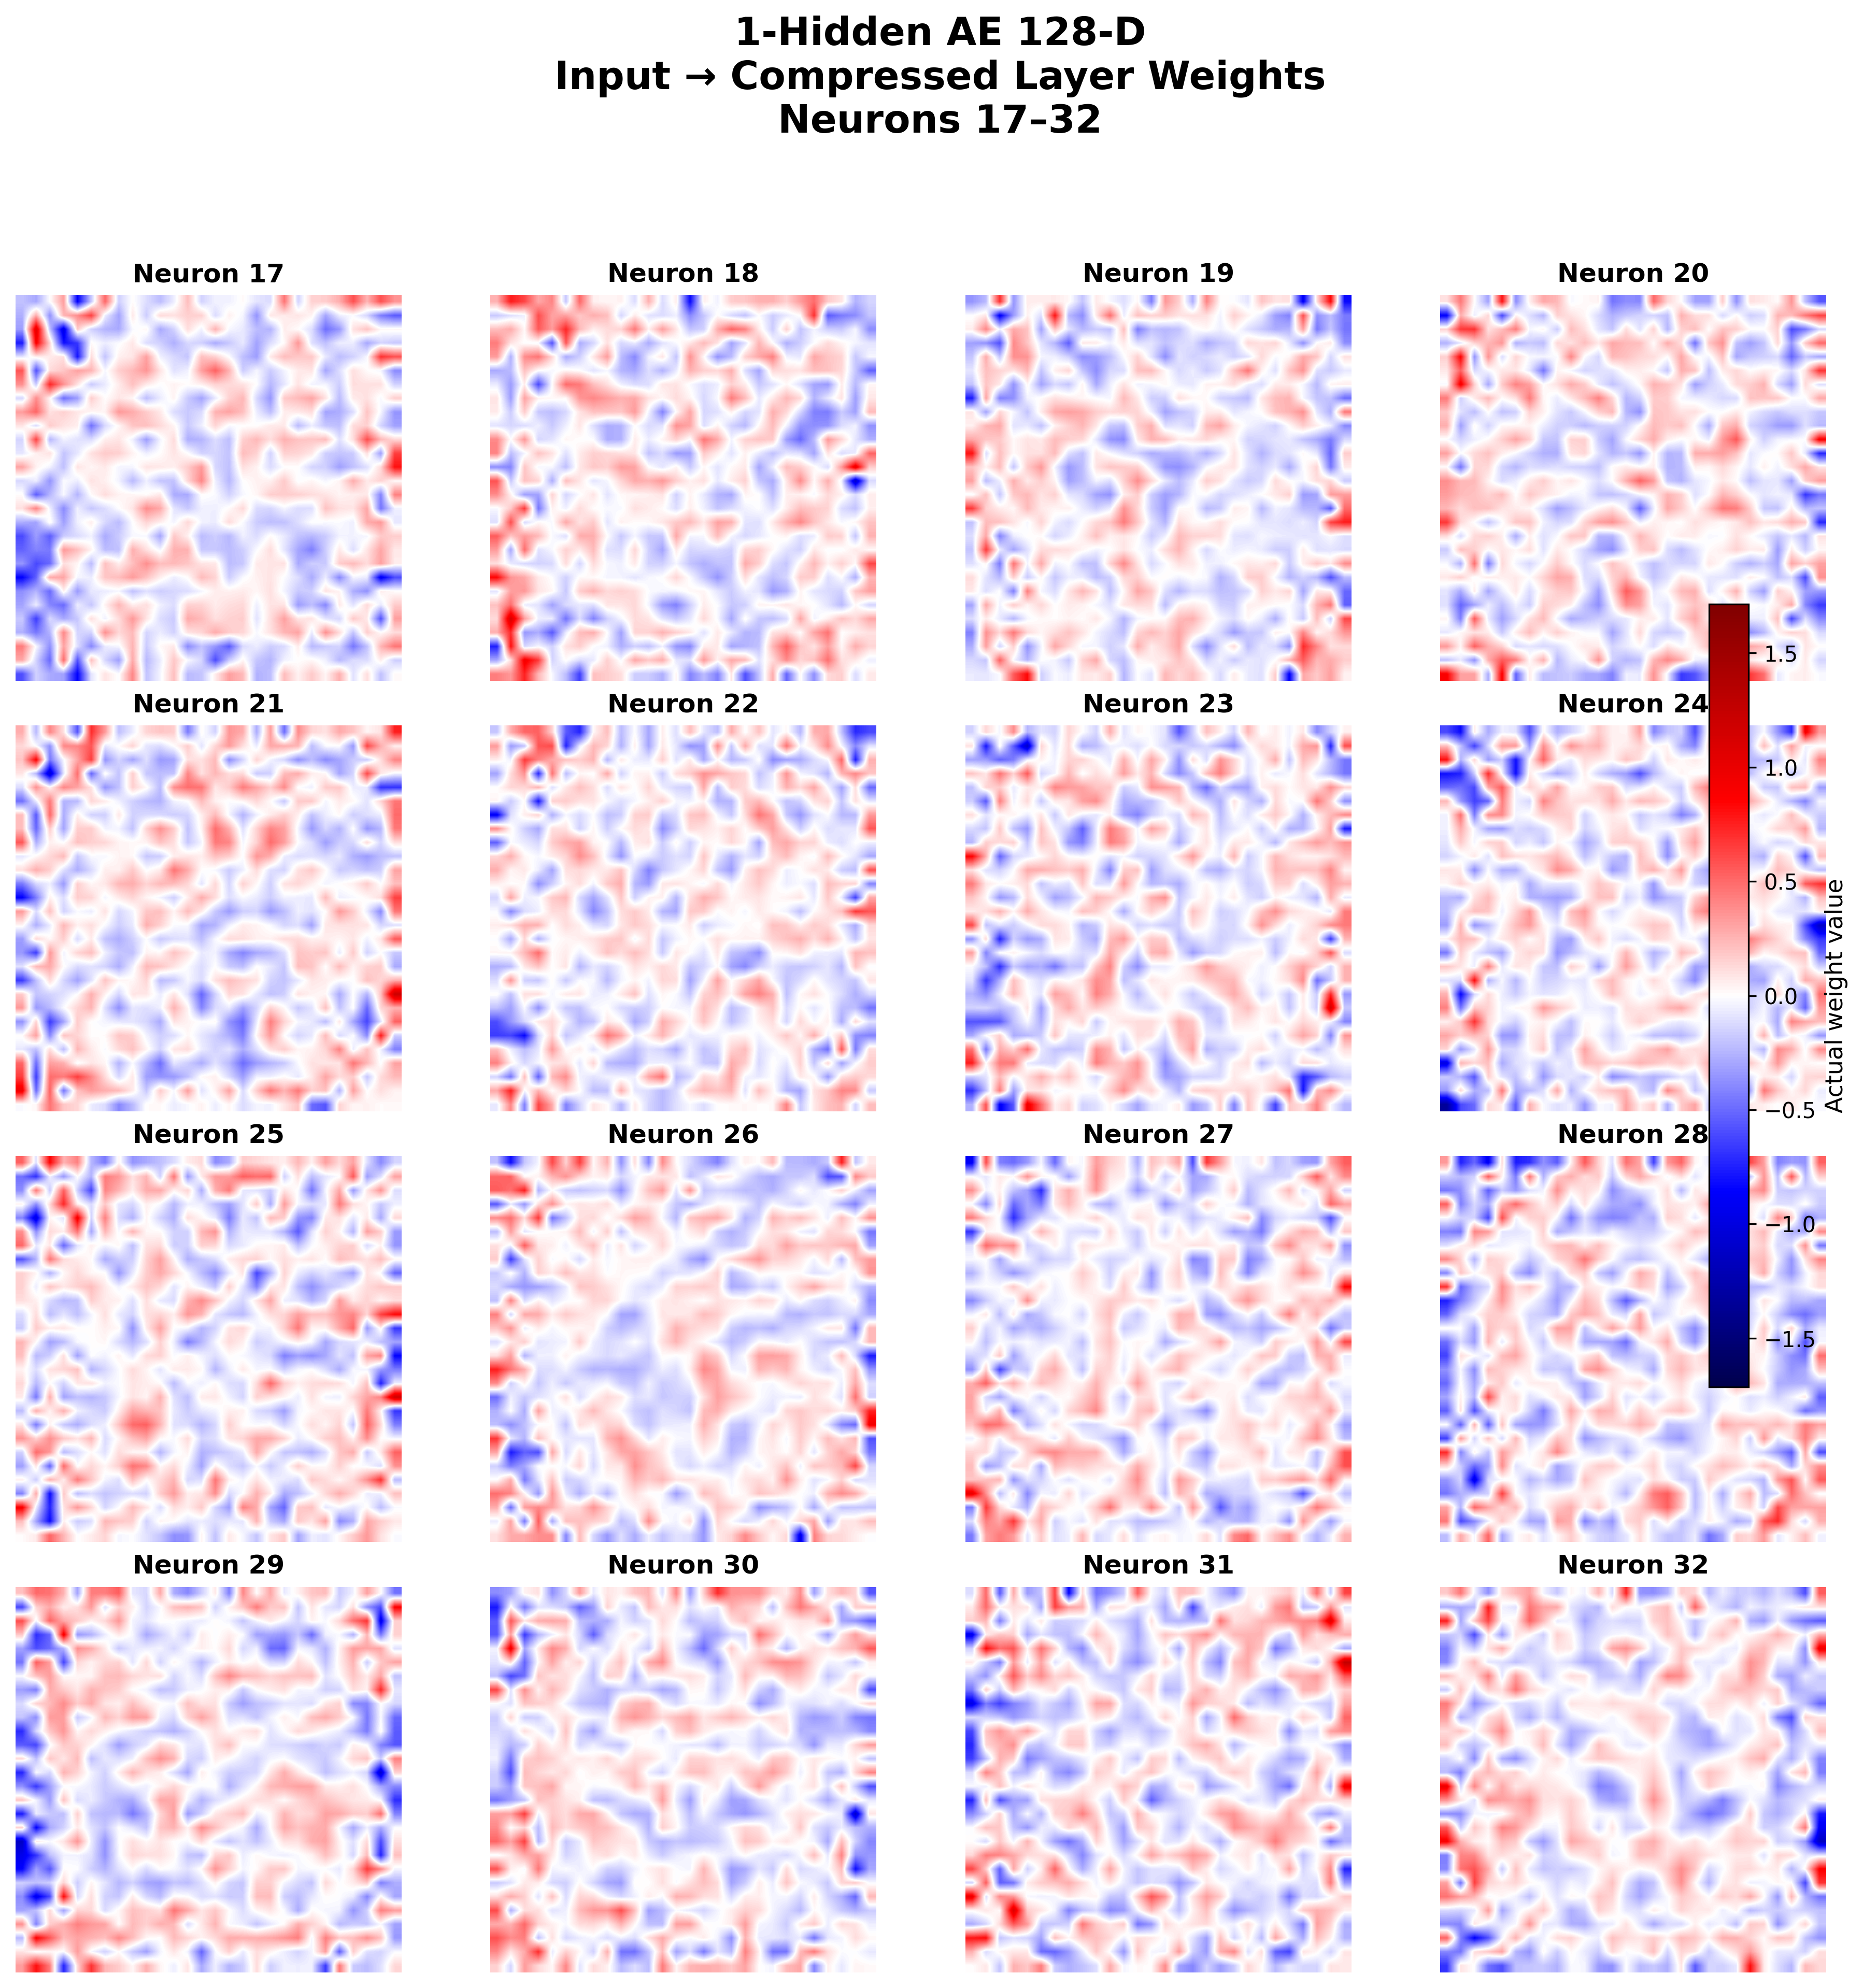
\includegraphics[width=0.99\linewidth,height=0.72\textheight,keepaspectratio]{figures/task6/1_hidden_ae/neurons_017_032.png}
\caption{Input-to-bottleneck weight visualization for neurons 17--32.}
\label{fig:task6_2}
\end{figure}

\begin{figure}[H]
\centering
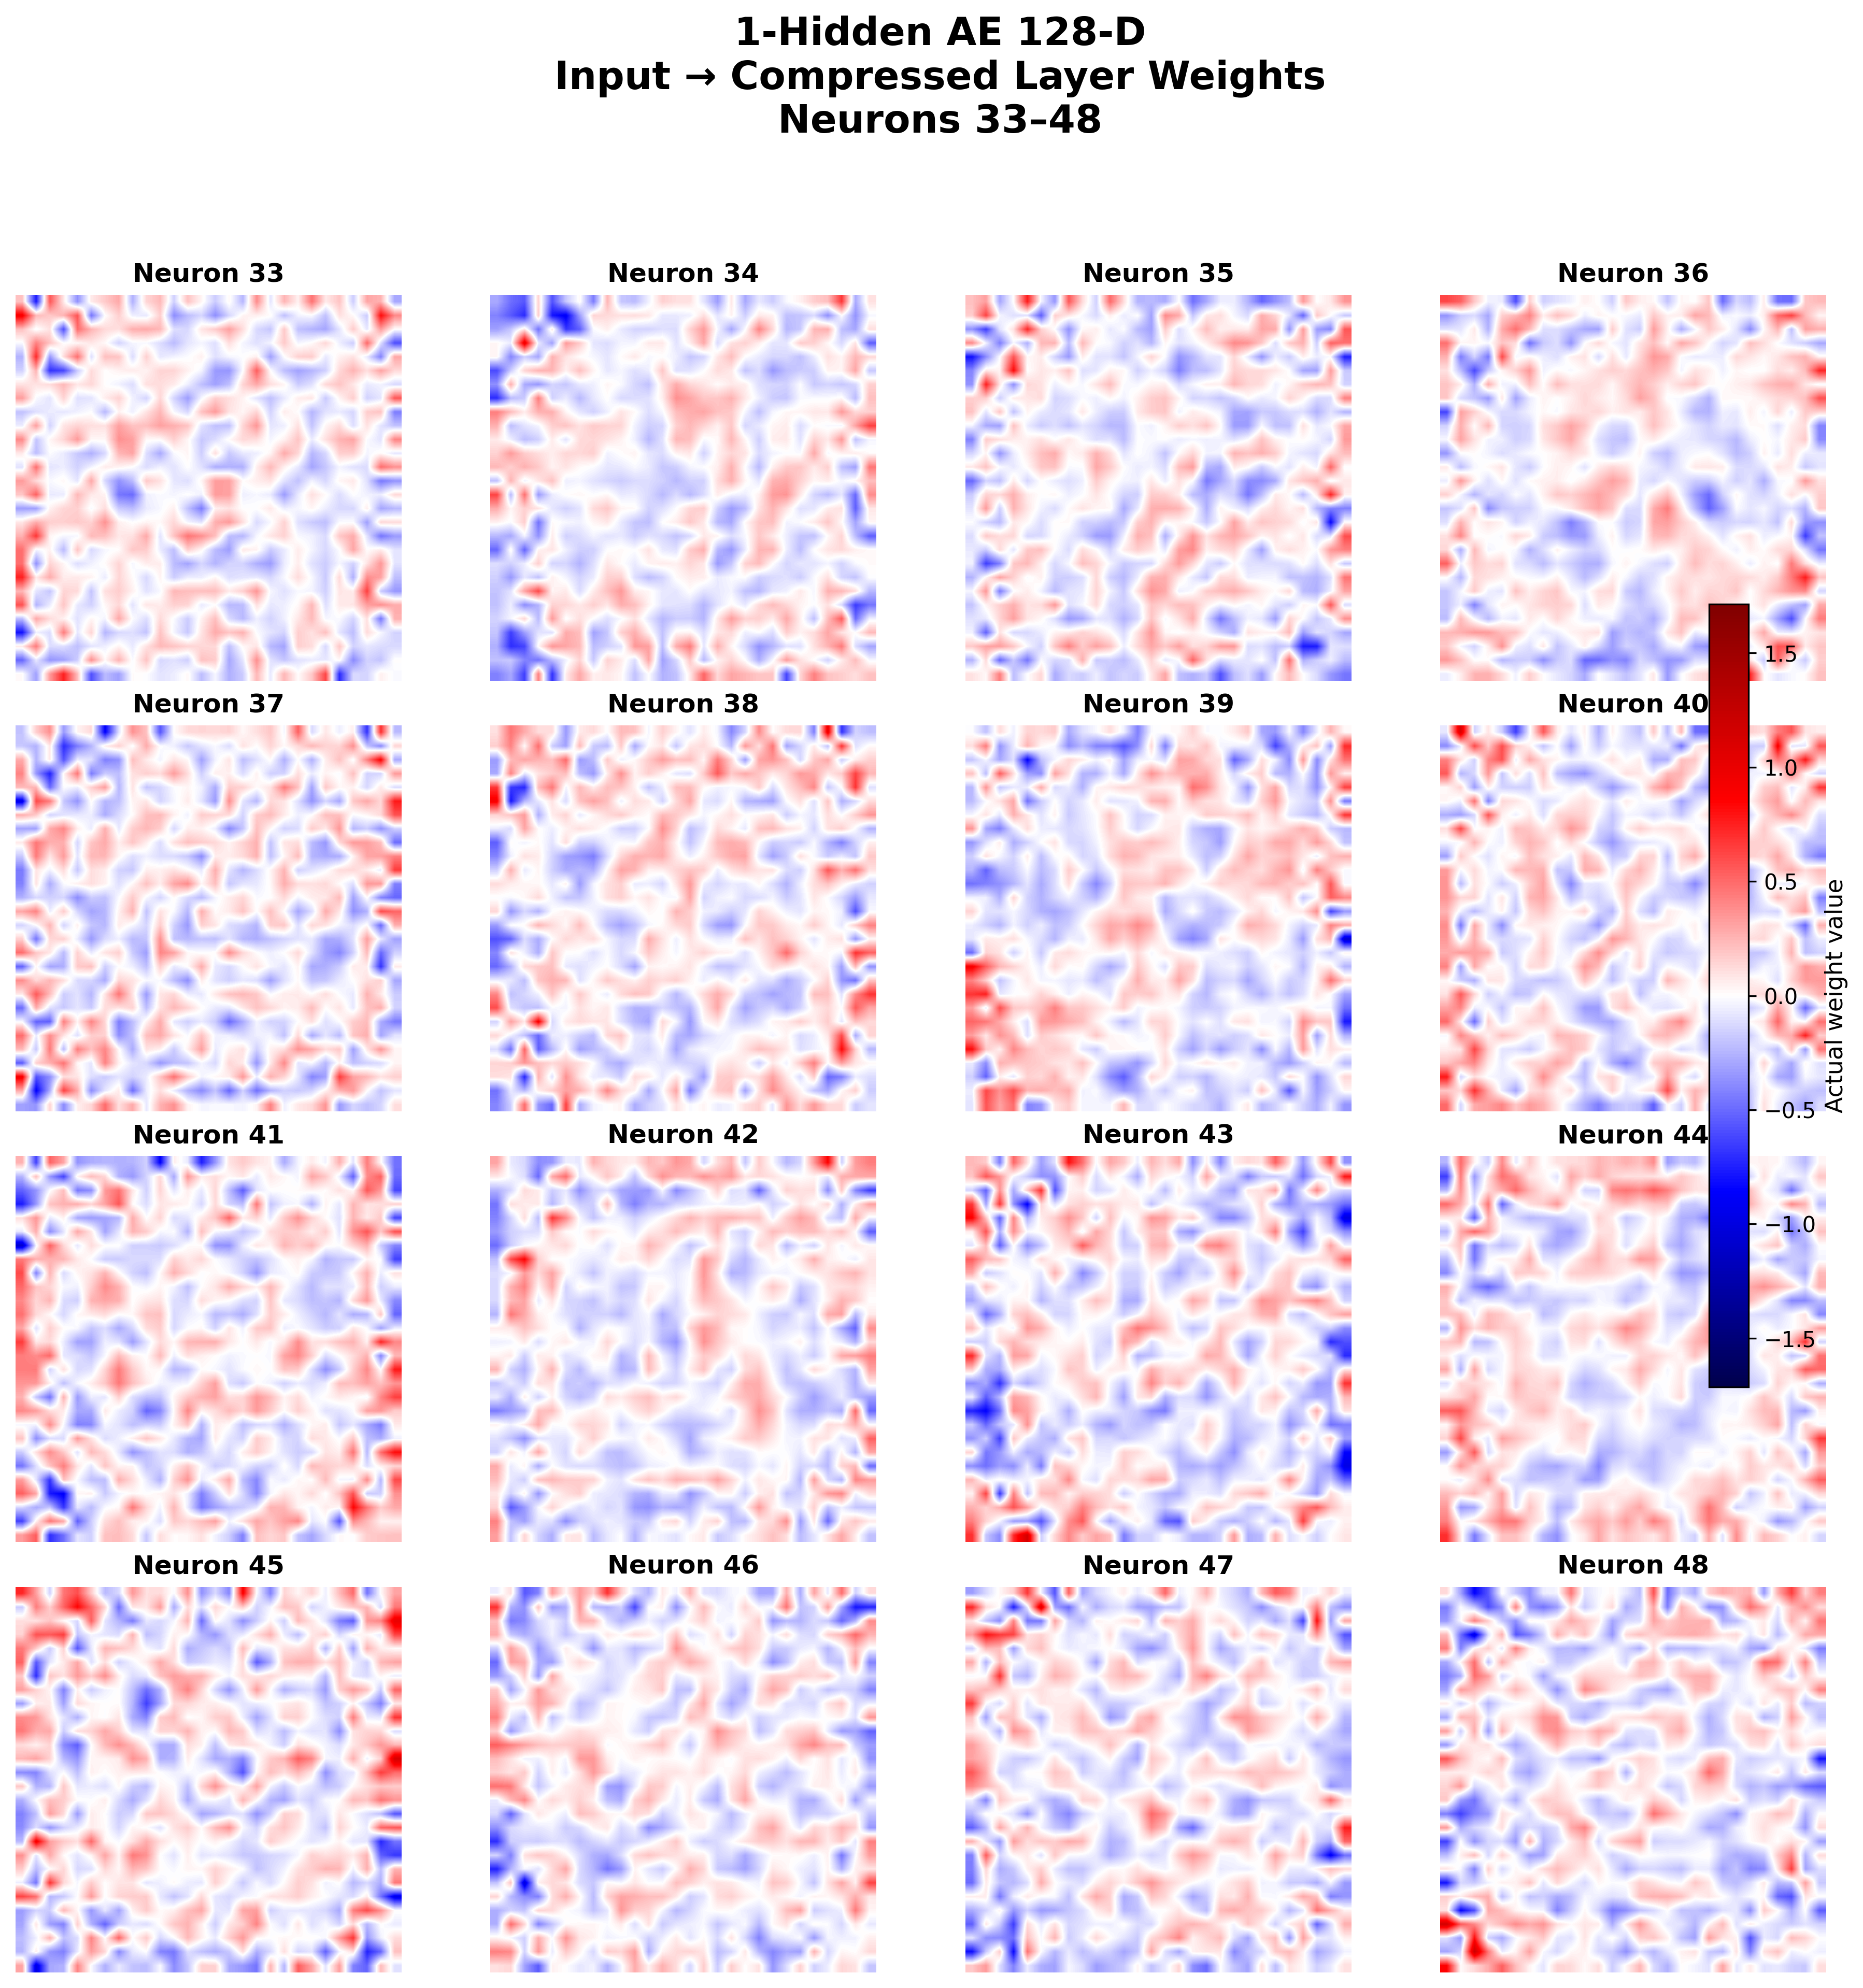
\includegraphics[width=0.99\linewidth,height=0.72\textheight,keepaspectratio]{figures/task6/1_hidden_ae/neurons_033_048.png}
\caption{Input-to-bottleneck weight visualization for neurons 33--48.}
\label{fig:task6_3}
\end{figure}

\begin{figure}[H]
\centering
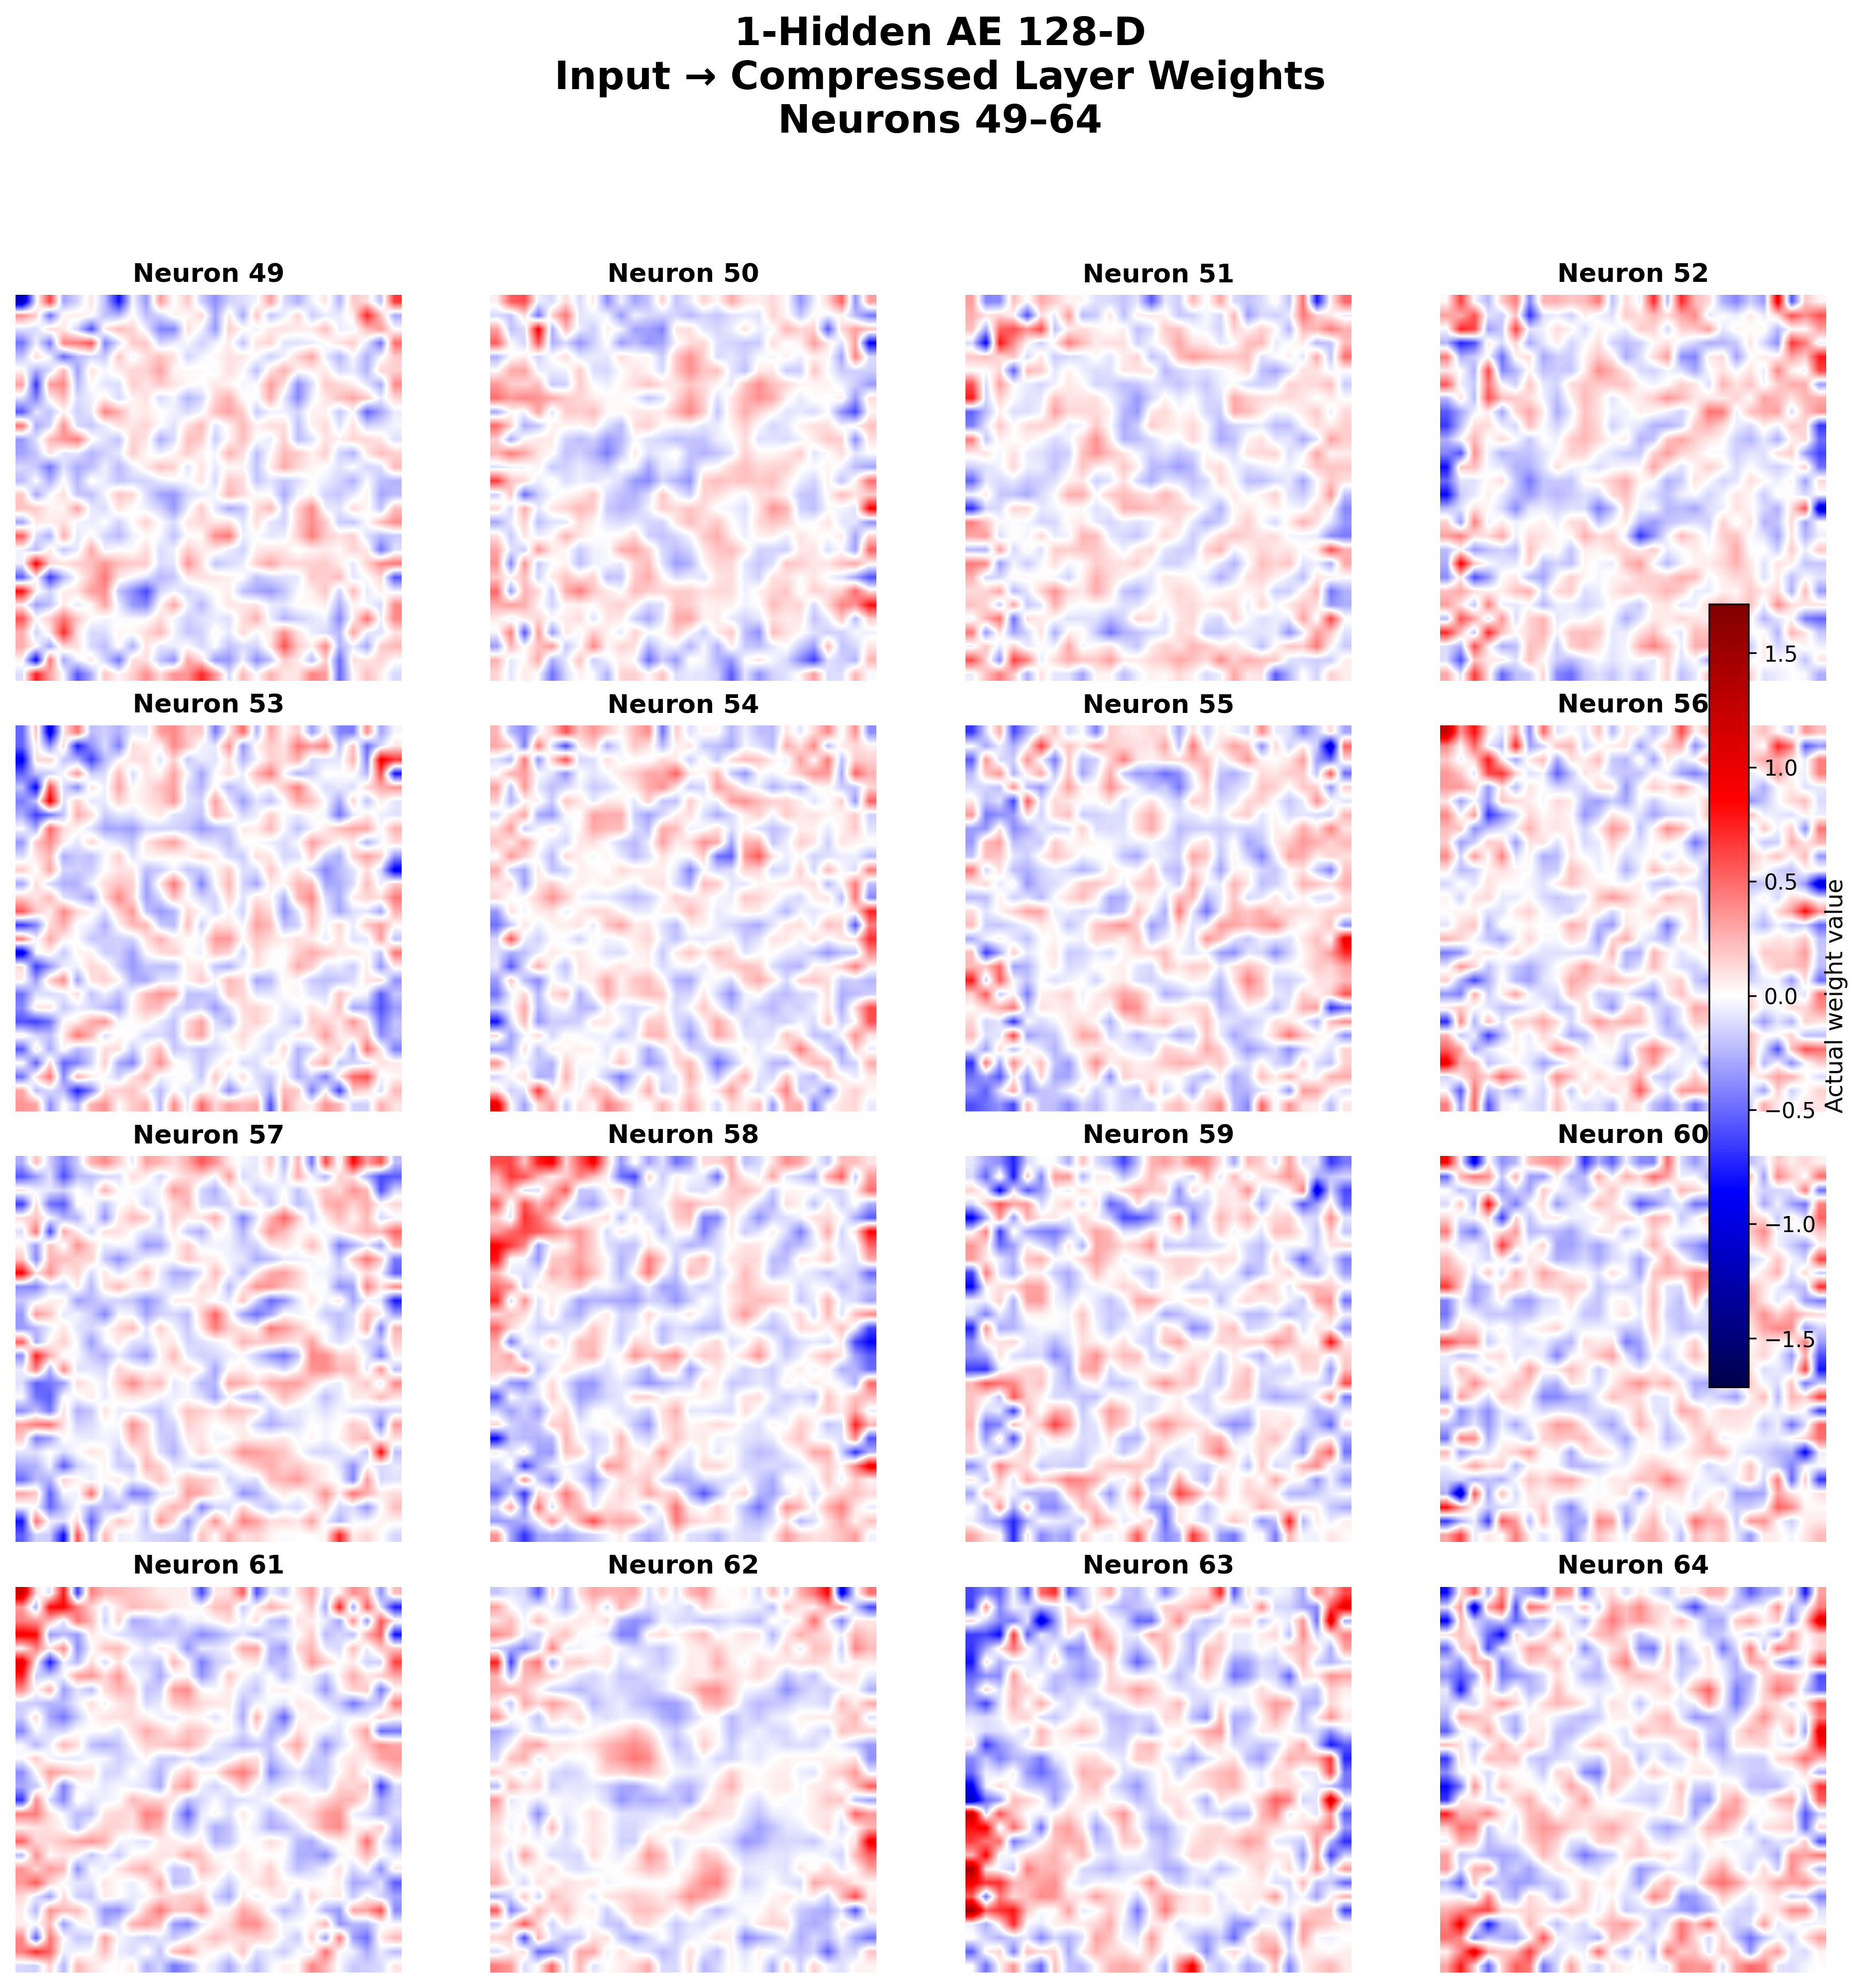
\includegraphics[width=0.99\linewidth,height=0.72\textheight,keepaspectratio]{figures/task6/1_hidden_ae/neurons_049_064.png}
\caption{Input-to-bottleneck weight visualization for neurons 49--64.}
\label{fig:task6_4}
\end{figure}

\begin{figure}[H]
\centering
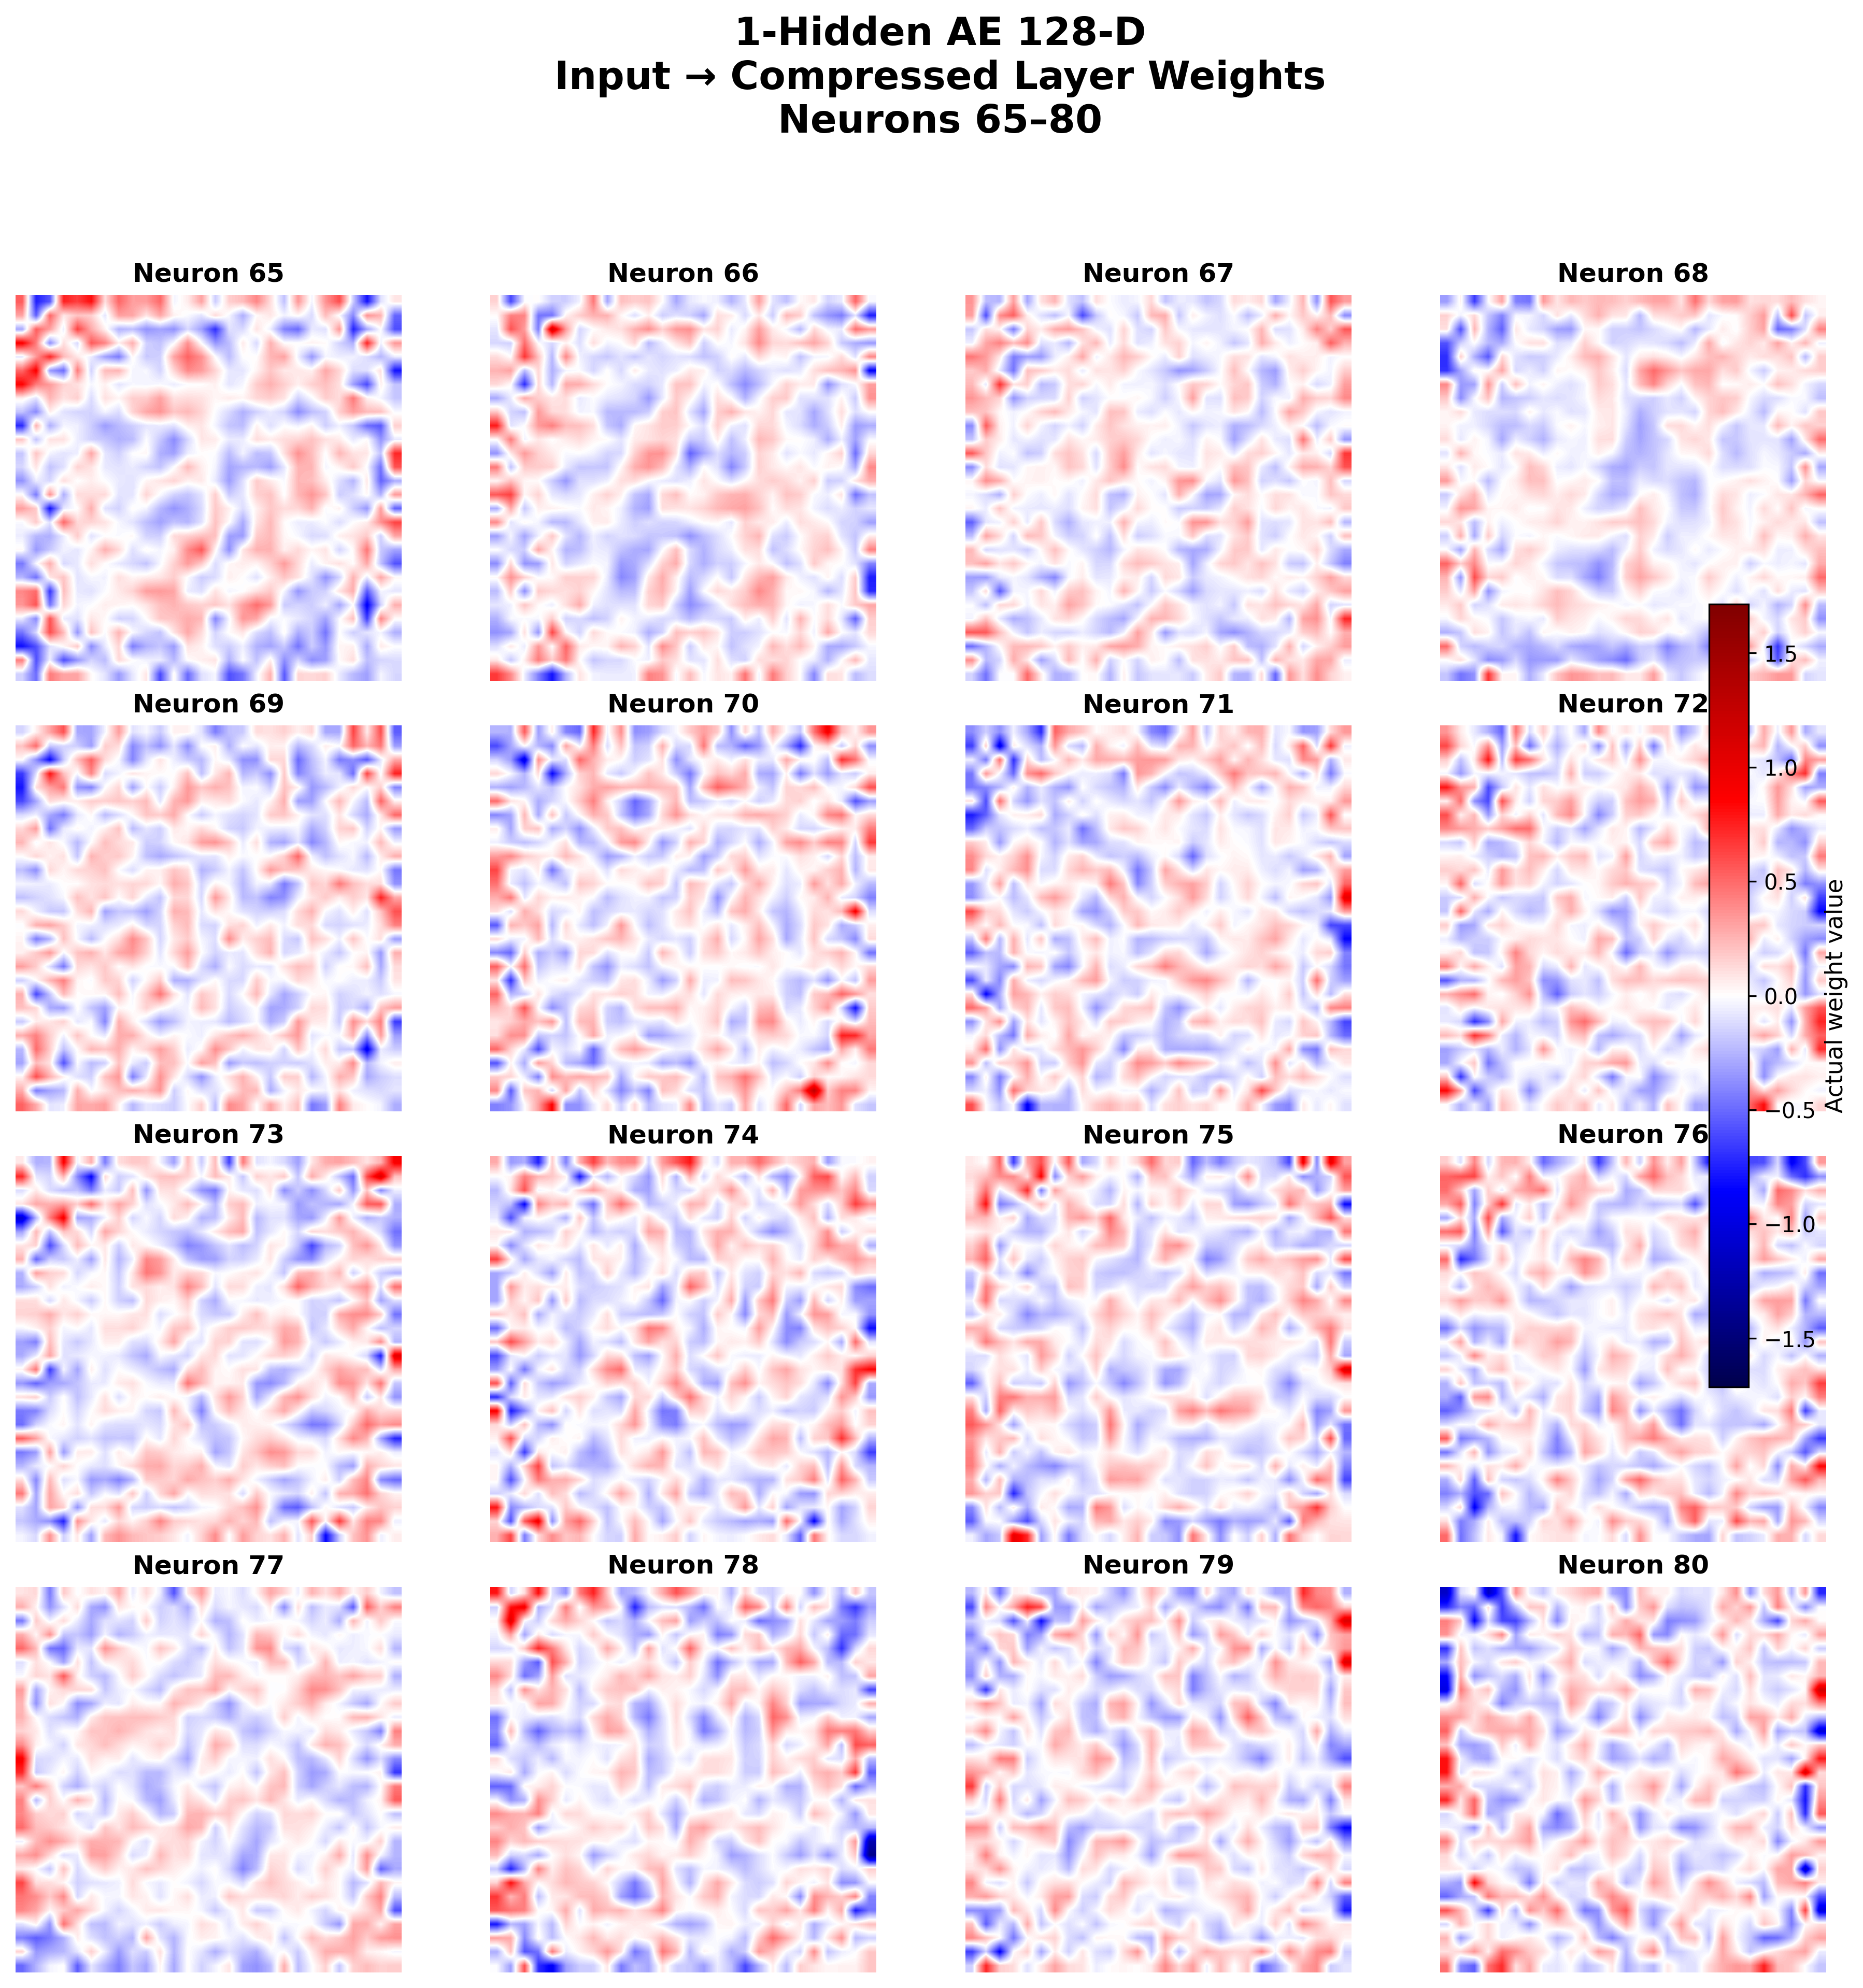
\includegraphics[width=0.99\linewidth,height=0.72\textheight,keepaspectratio]{figures/task6/1_hidden_ae/neurons_065_080.png}
\caption{Input-to-bottleneck weight visualization for neurons 65--80.}
\label{fig:task6_5}
\end{figure}

\begin{figure}[H]
\centering
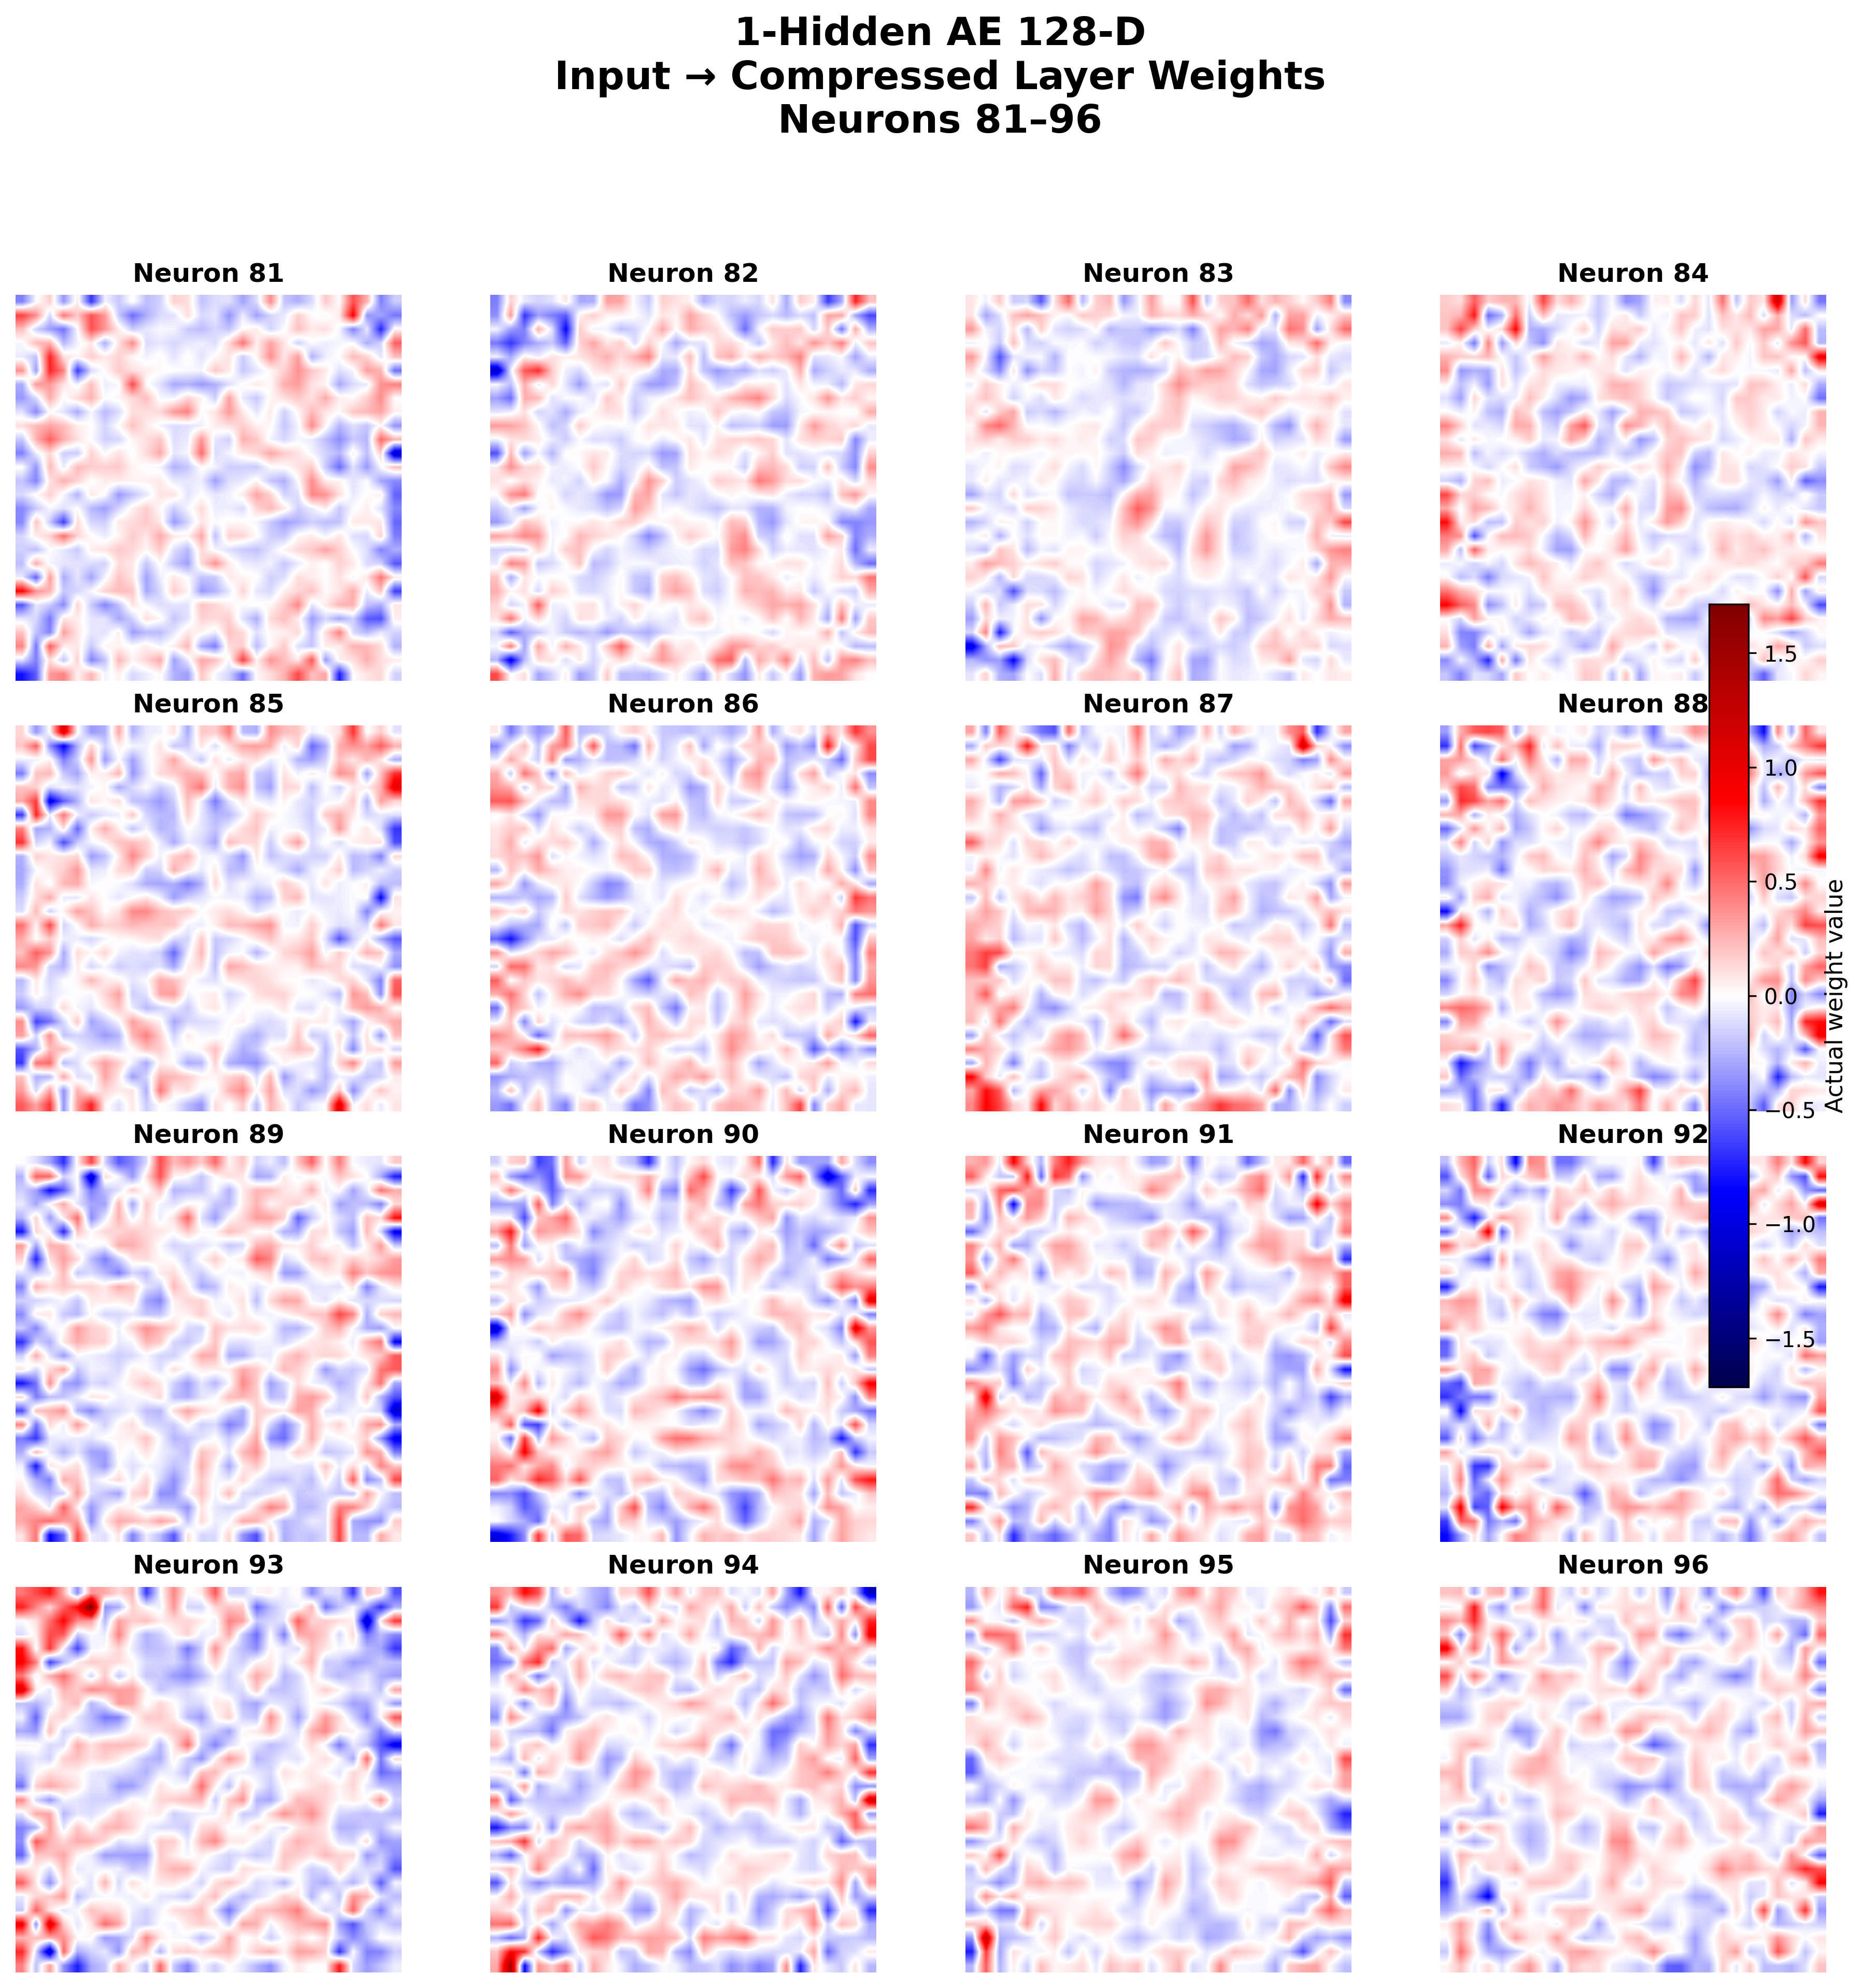
\includegraphics[width=0.99\linewidth,height=0.72\textheight,keepaspectratio]{figures/task6/1_hidden_ae/neurons_081_096.png}
\caption{Input-to-bottleneck weight visualization for neurons 81--96.}
\label{fig:task6_6}
\end{figure}

\begin{figure}[H]
\centering
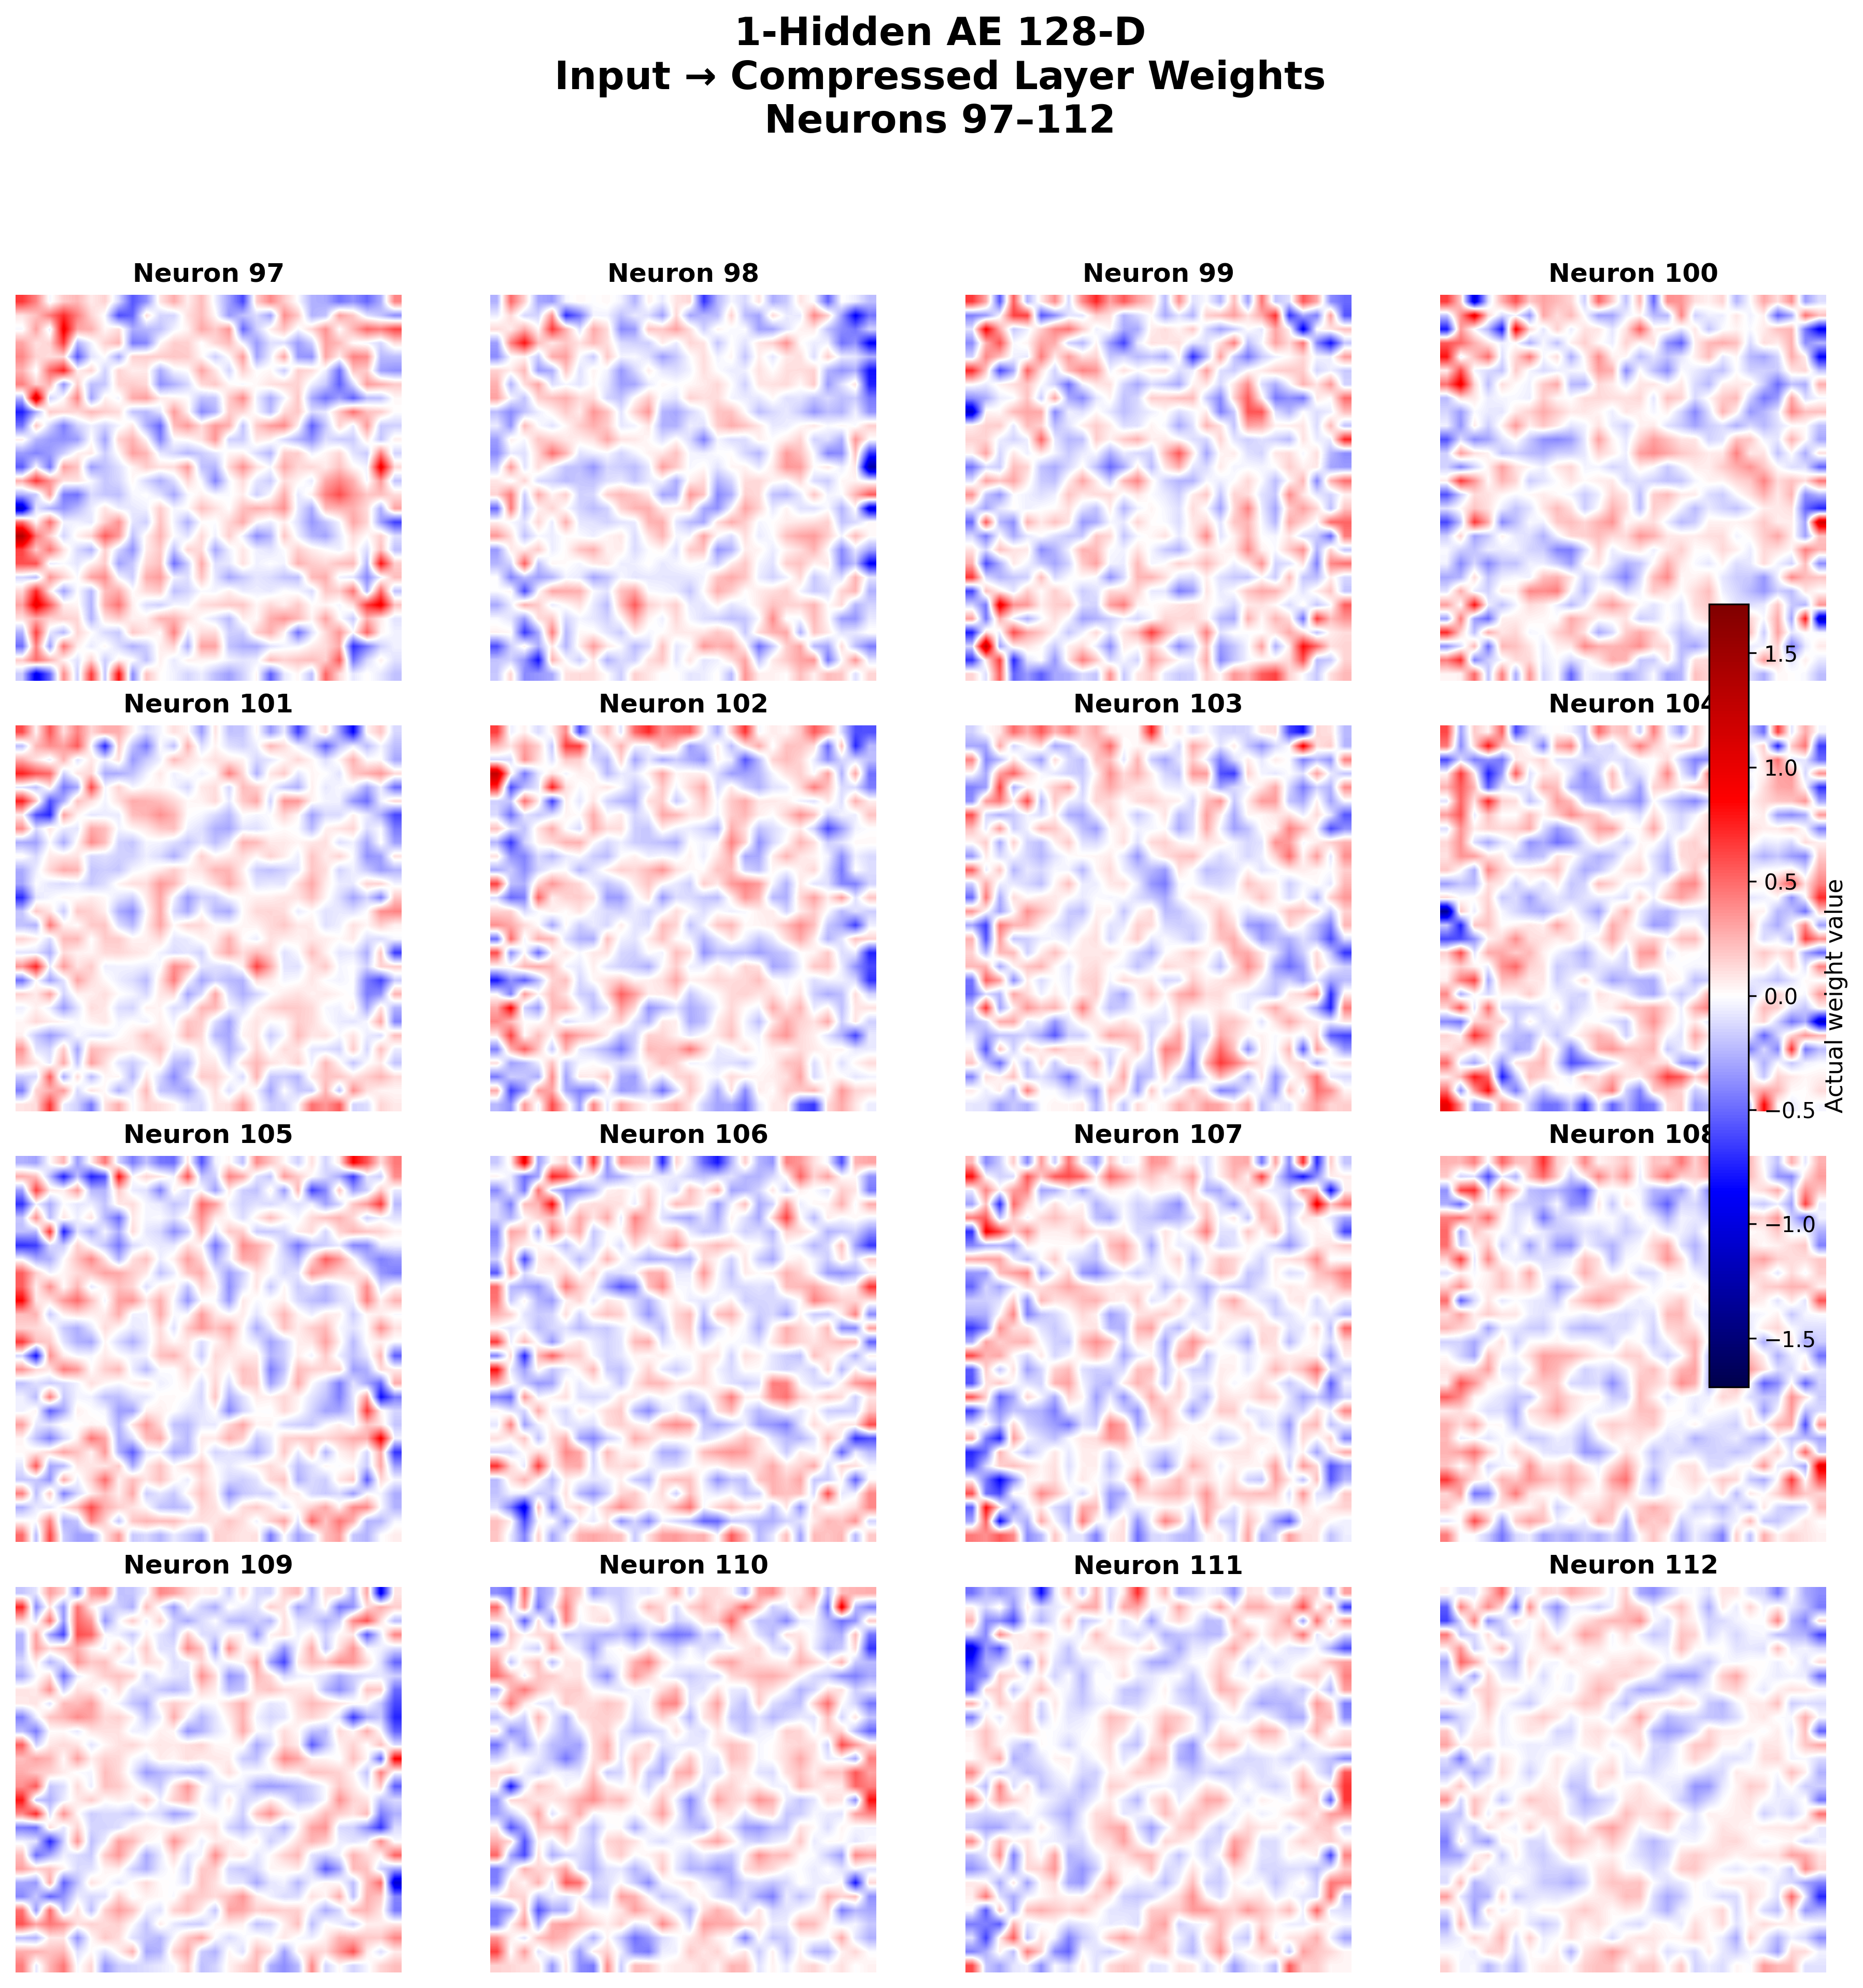
\includegraphics[width=0.99\linewidth,height=0.72\textheight,keepaspectratio]{figures/task6/1_hidden_ae/neurons_097_112.png}
\caption{Input-to-bottleneck weight visualization for neurons 97--112.}
\label{fig:task6_7}
\end{figure}

\begin{figure}[H]
\centering
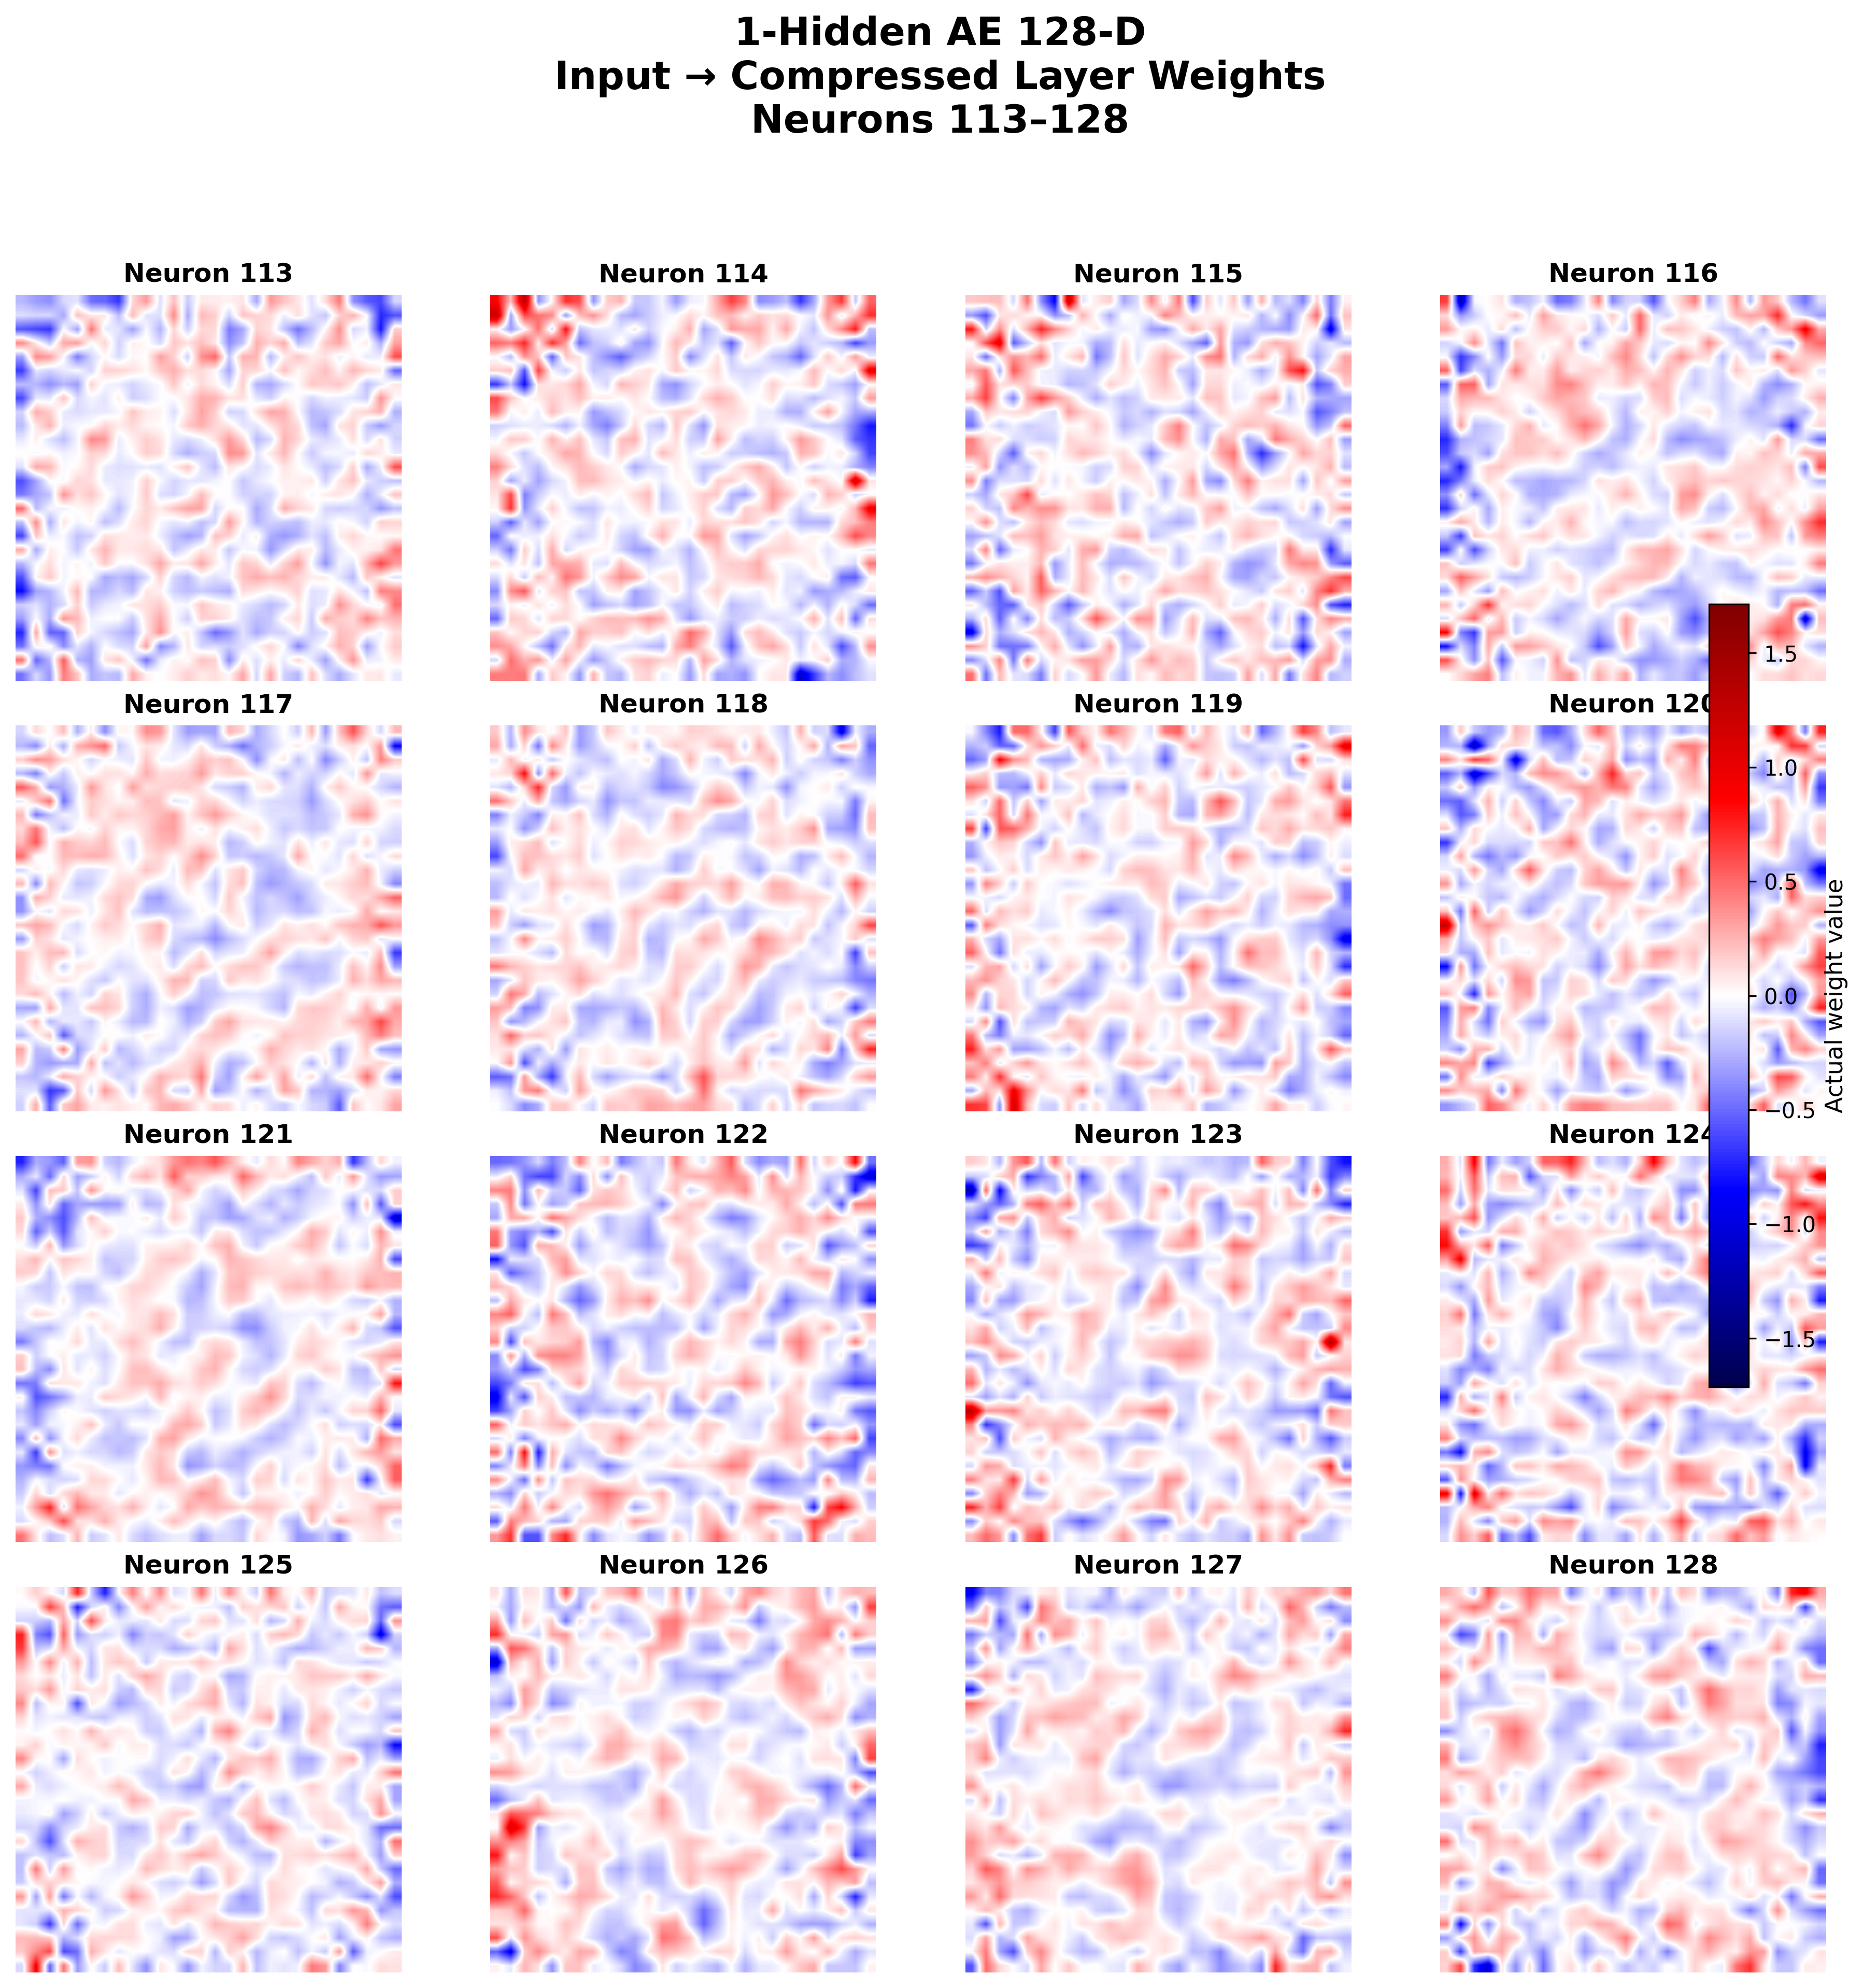
\includegraphics[width=0.99\linewidth,height=0.72\textheight,keepaspectratio]{figures/task6/1_hidden_ae/neurons_113_128.png}
\caption{Input-to-bottleneck weight visualization for neurons 113--128.}
\label{fig:task6_8}
\end{figure}

\begin{figure}[H]
\centering
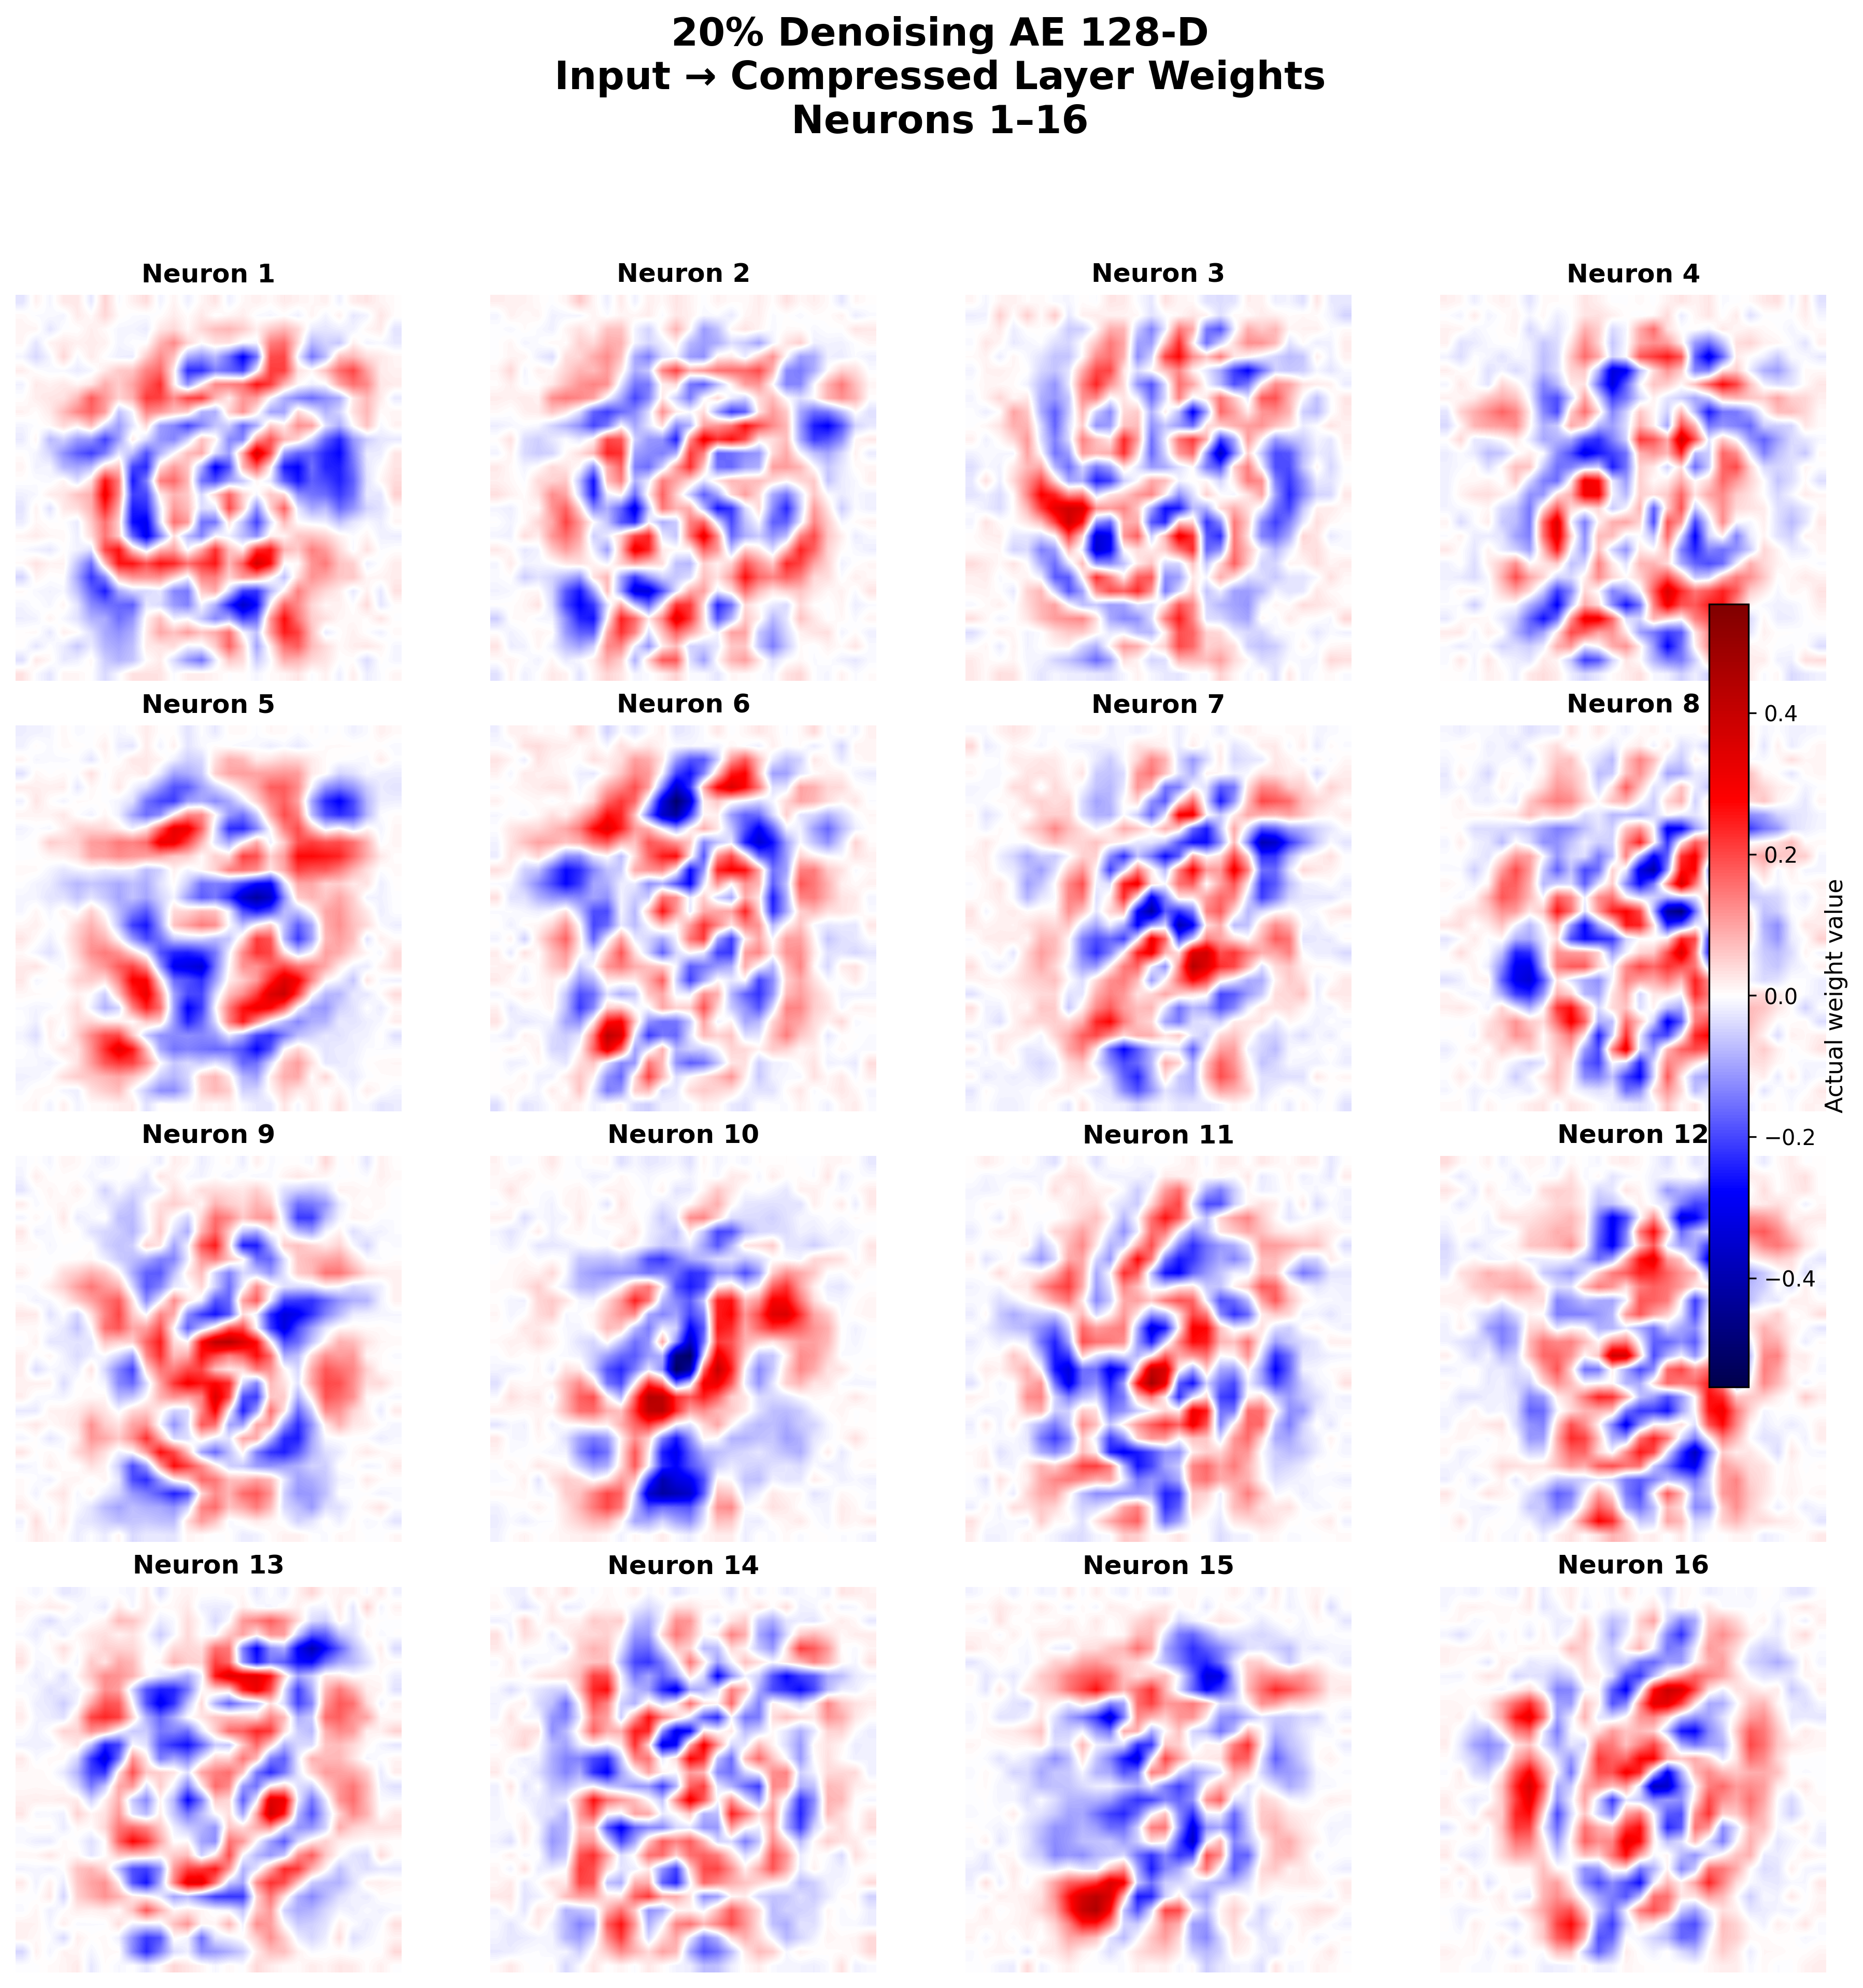
\includegraphics[width=0.99\linewidth,height=0.72\textheight,keepaspectratio]{figures/task6/20_pct_dae/neurons_001_016.png}
\caption{Input-to-bottleneck weight visualization for neurons 1--16.}
\label{fig:task6_9}
\end{figure}

\begin{figure}[H]
\centering
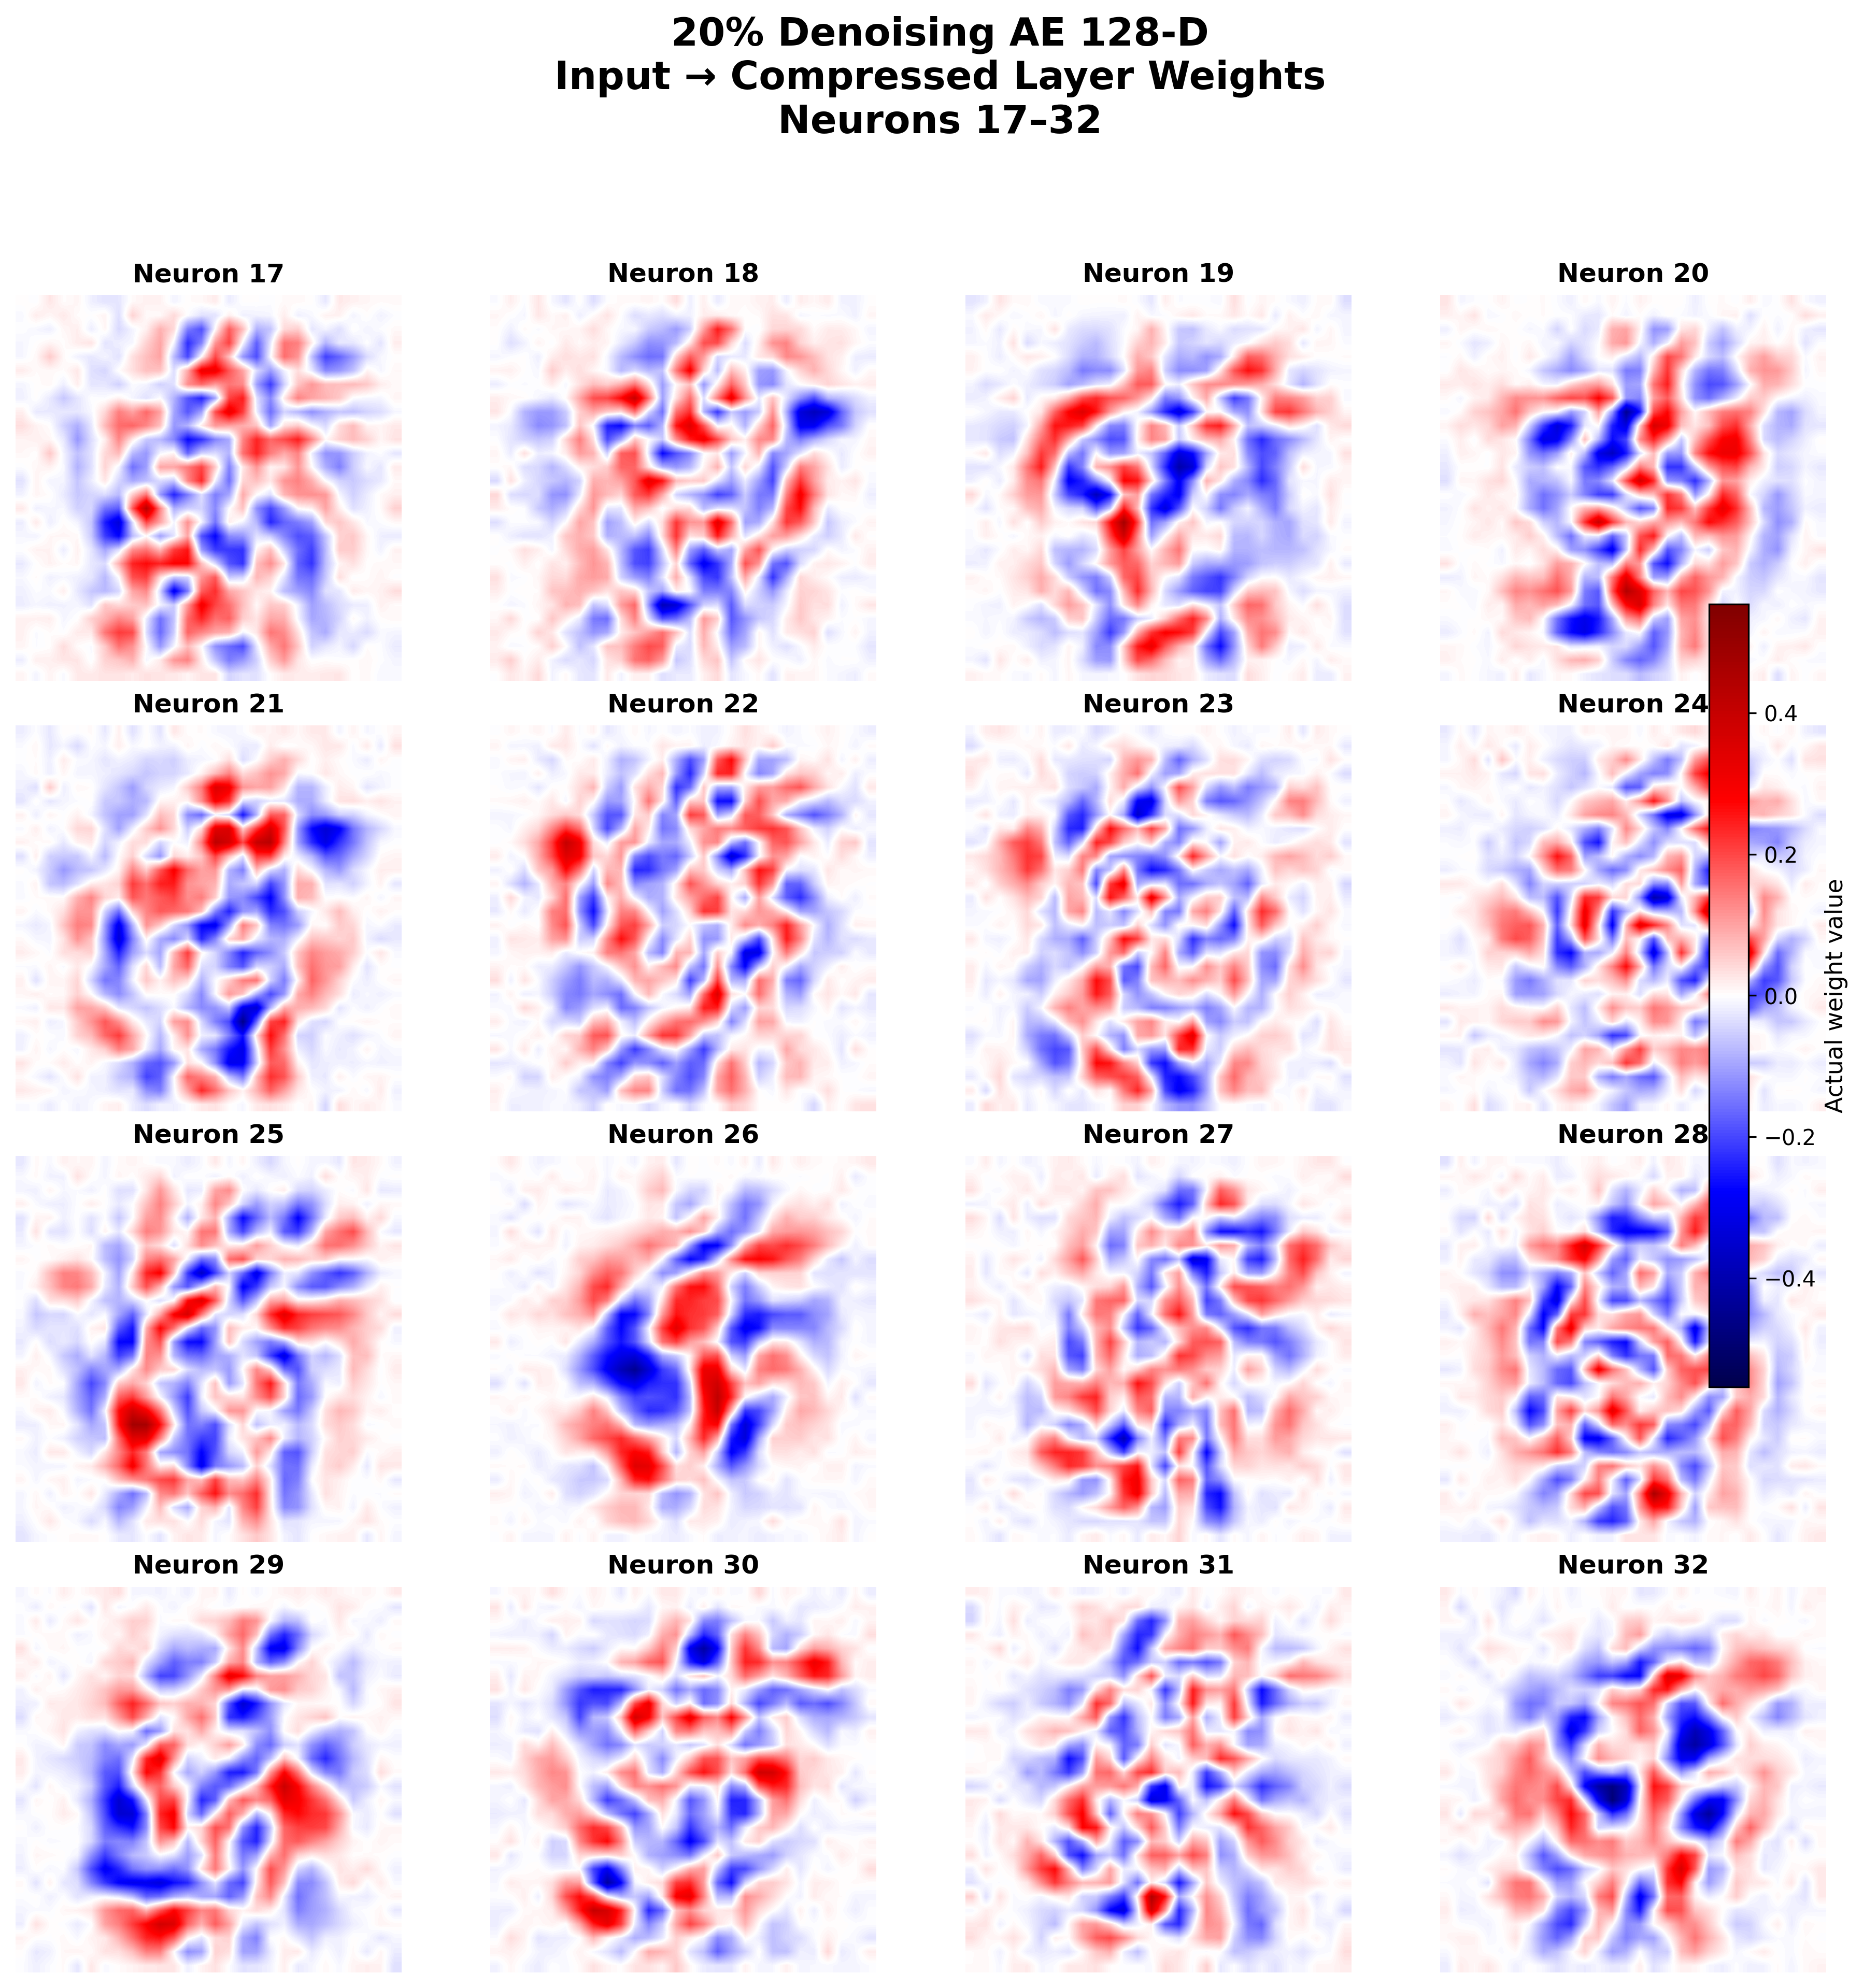
\includegraphics[width=0.99\linewidth,height=0.72\textheight,keepaspectratio]{figures/task6/20_pct_dae/neurons_017_032.png}
\caption{Input-to-bottleneck weight visualization for neurons 17--32.}
\label{fig:task6_10}
\end{figure}

\begin{figure}[H]
\centering
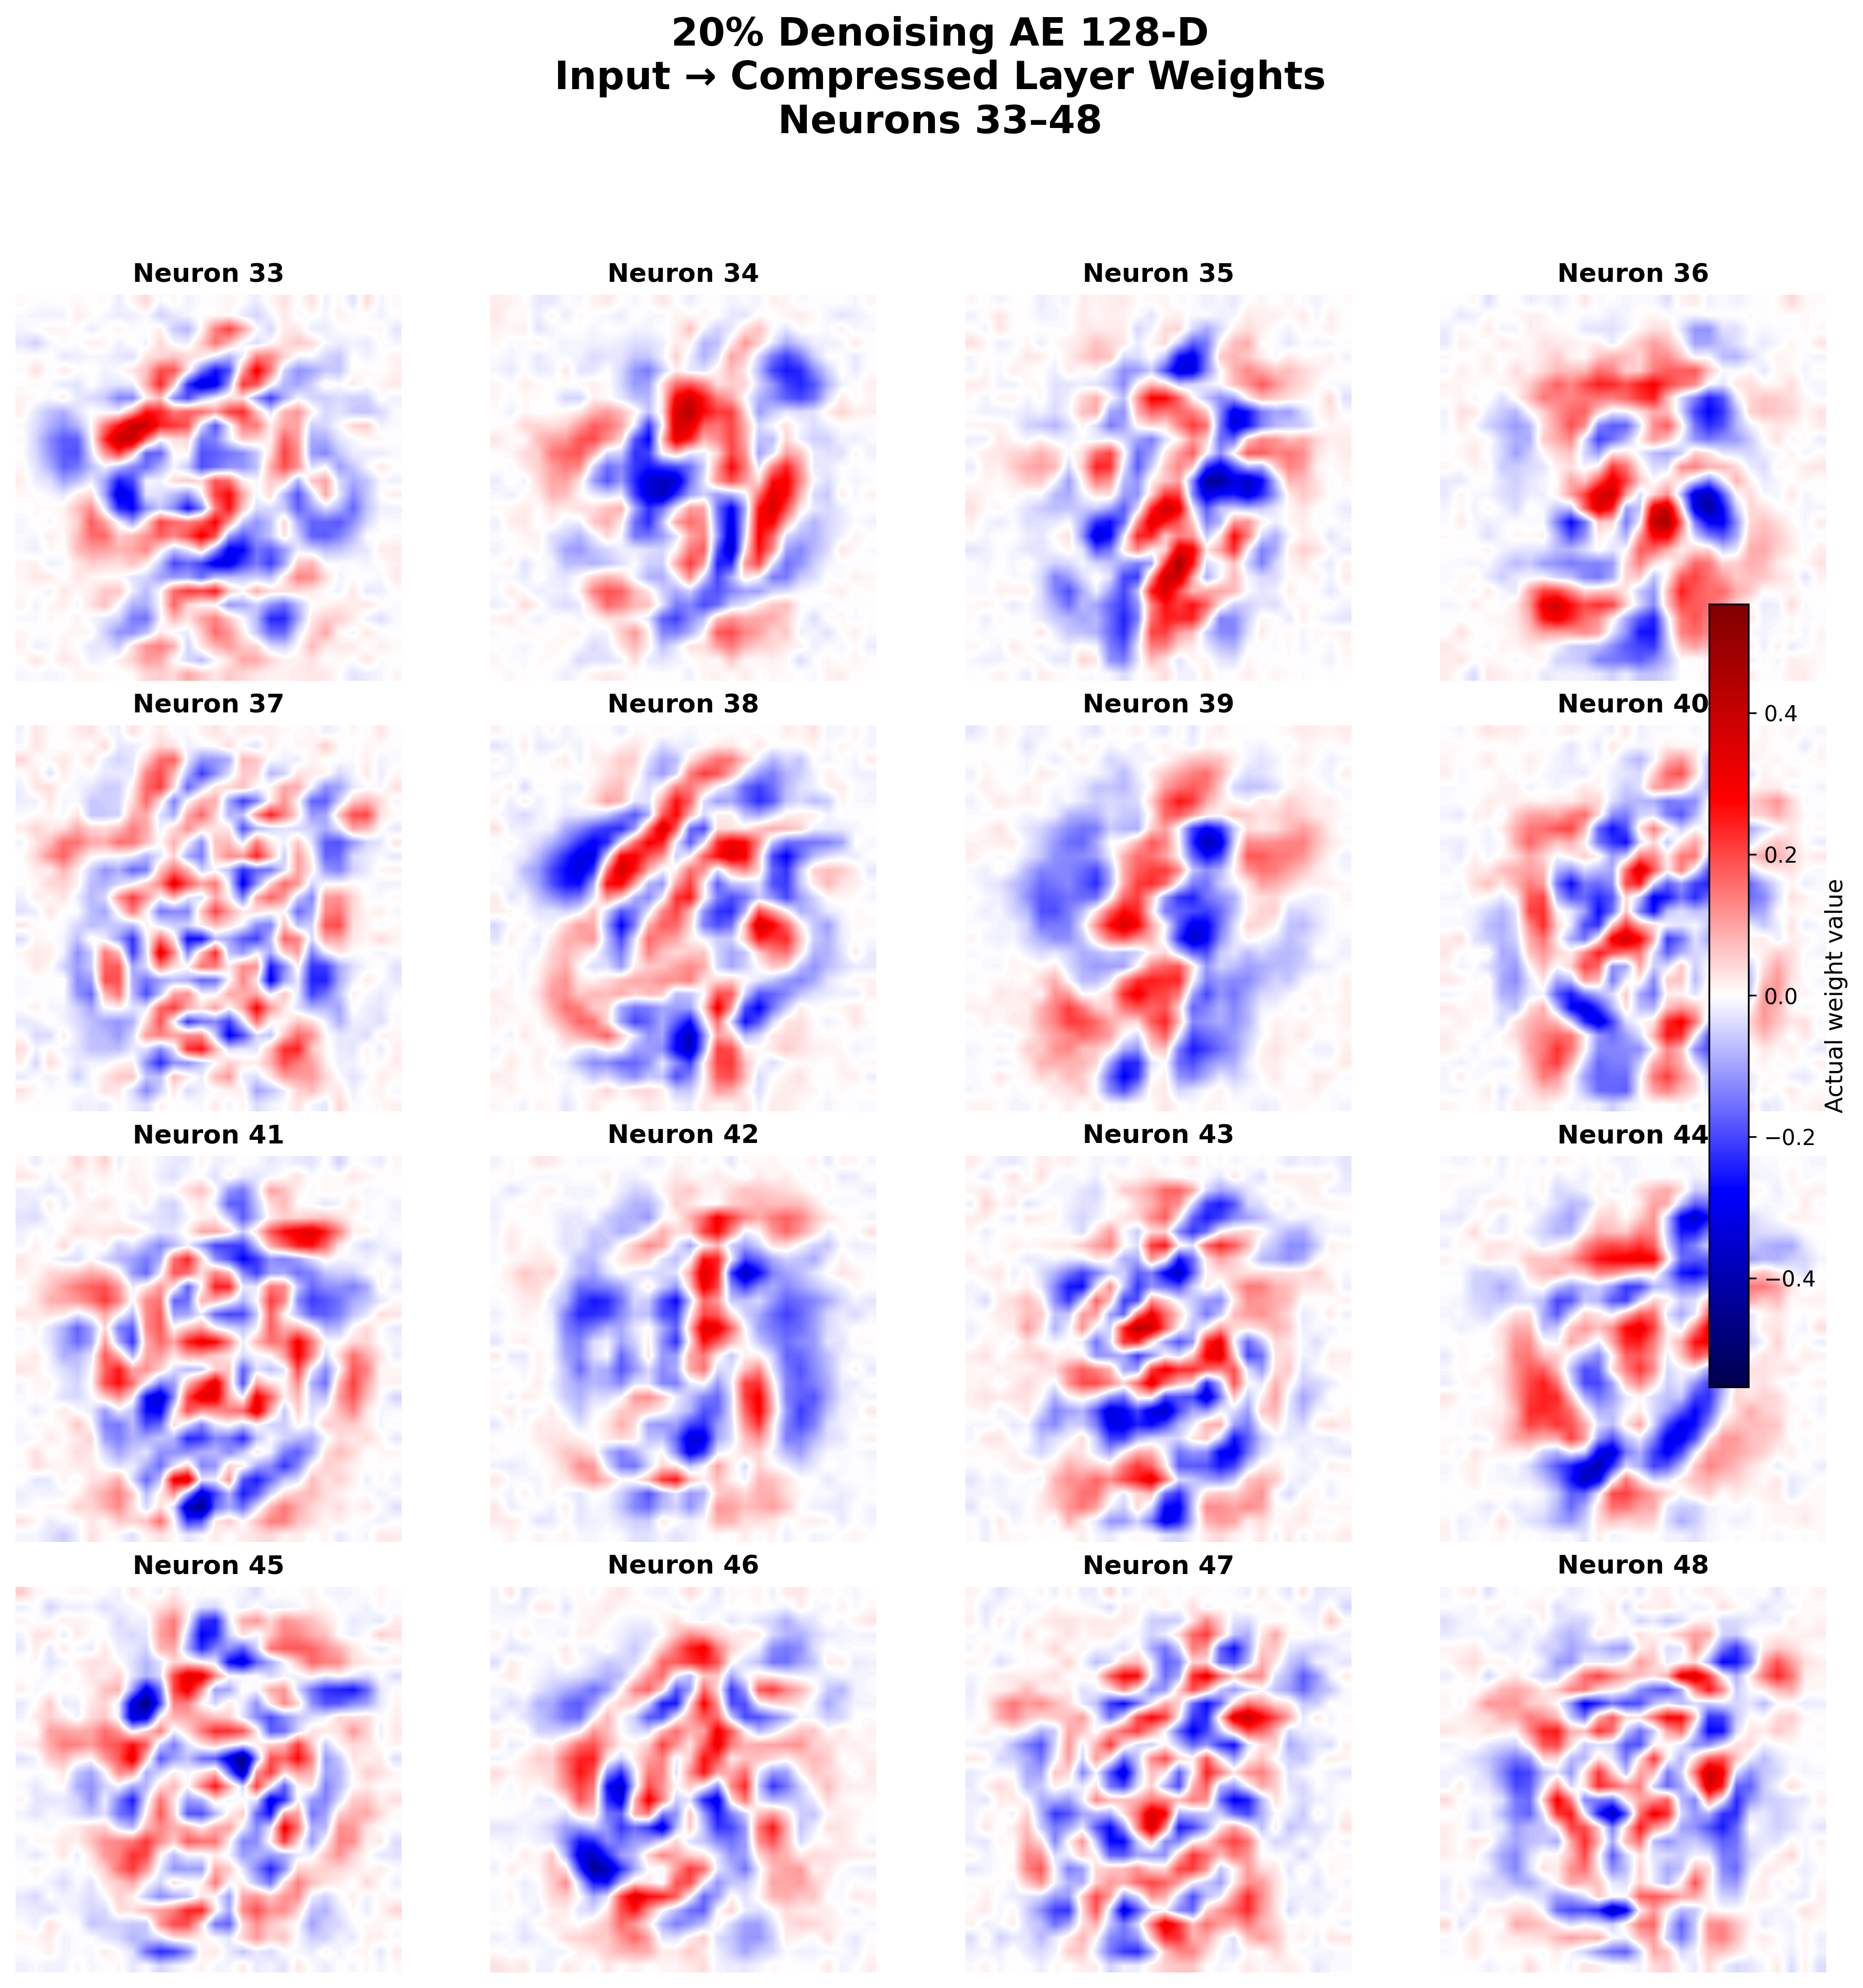
\includegraphics[width=0.99\linewidth,height=0.72\textheight,keepaspectratio]{figures/task6/20_pct_dae/neurons_033_048.png}
\caption{Input-to-bottleneck weight visualization for neurons 33--48.}
\label{fig:task6_11}
\end{figure}

\begin{figure}[H]
\centering
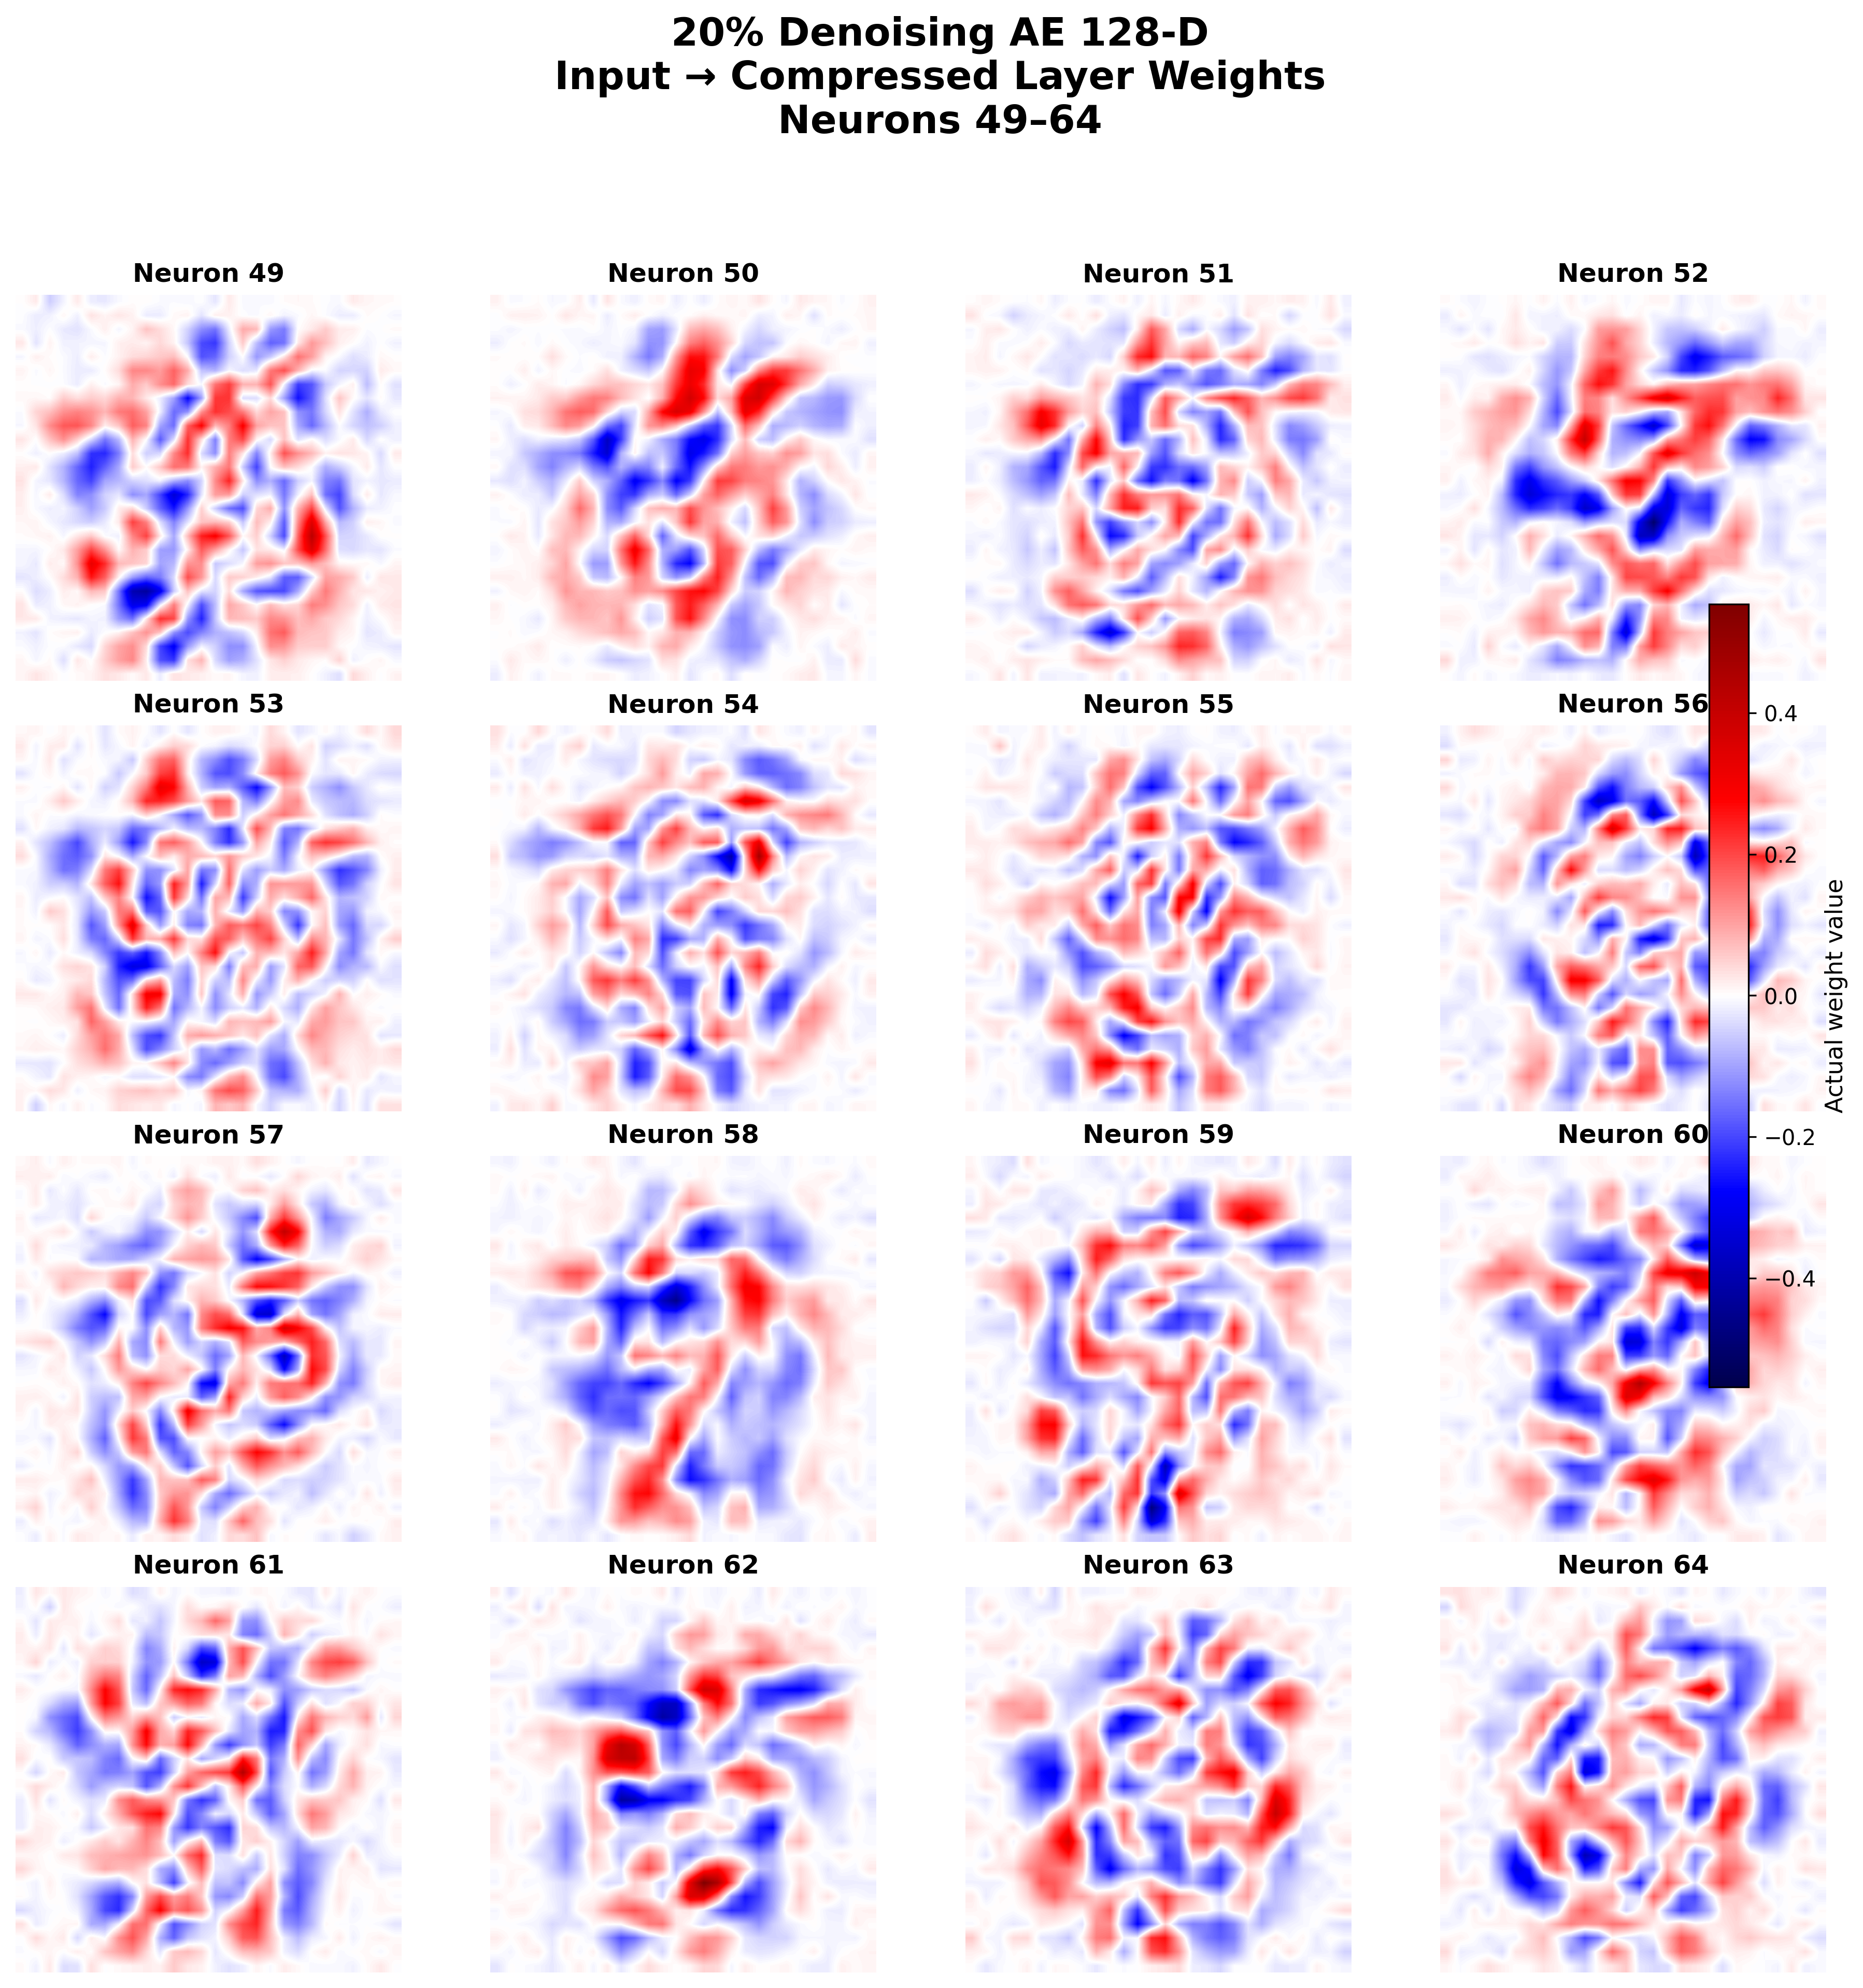
\includegraphics[width=0.99\linewidth,height=0.72\textheight,keepaspectratio]{figures/task6/20_pct_dae/neurons_049_064.png}
\caption{Input-to-bottleneck weight visualization for neurons 49--64.}
\label{fig:task6_12}
\end{figure}

\begin{figure}[H]
\centering
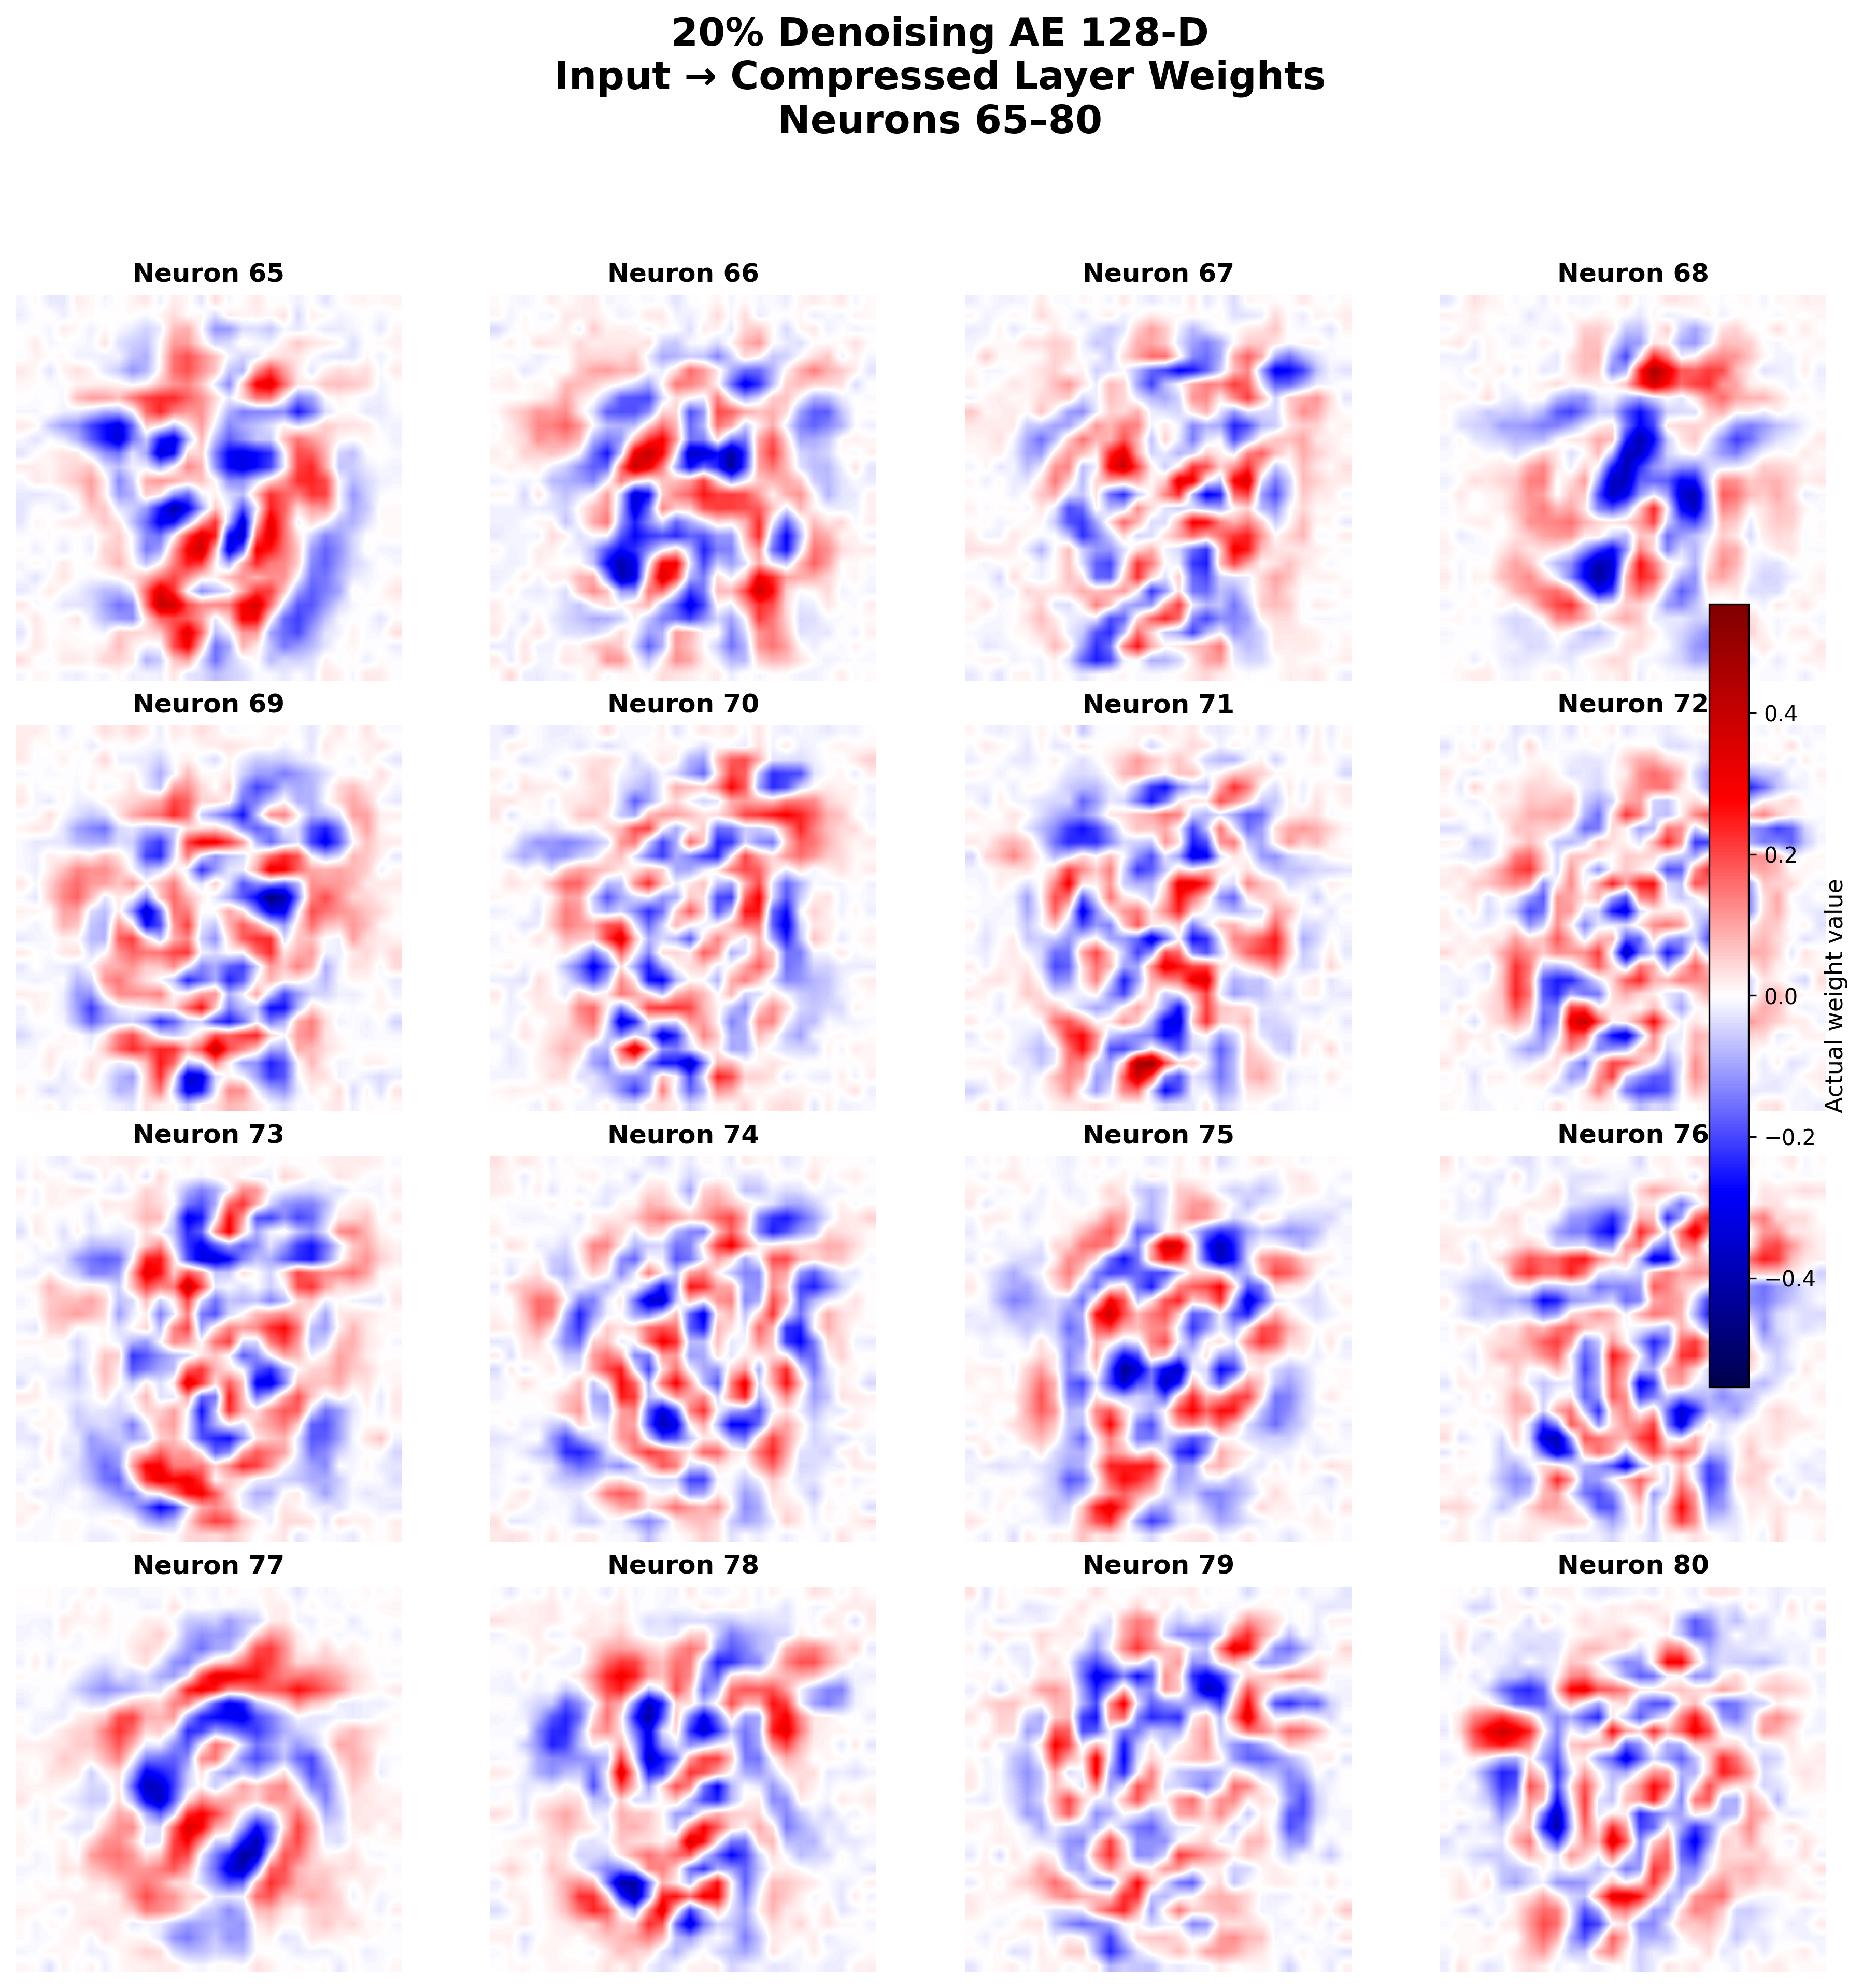
\includegraphics[width=0.99\linewidth,height=0.72\textheight,keepaspectratio]{figures/task6/20_pct_dae/neurons_065_080.png}
\caption{Input-to-bottleneck weight visualization for neurons 65--80.}
\label{fig:task6_13}
\end{figure}

\begin{figure}[H]
\centering
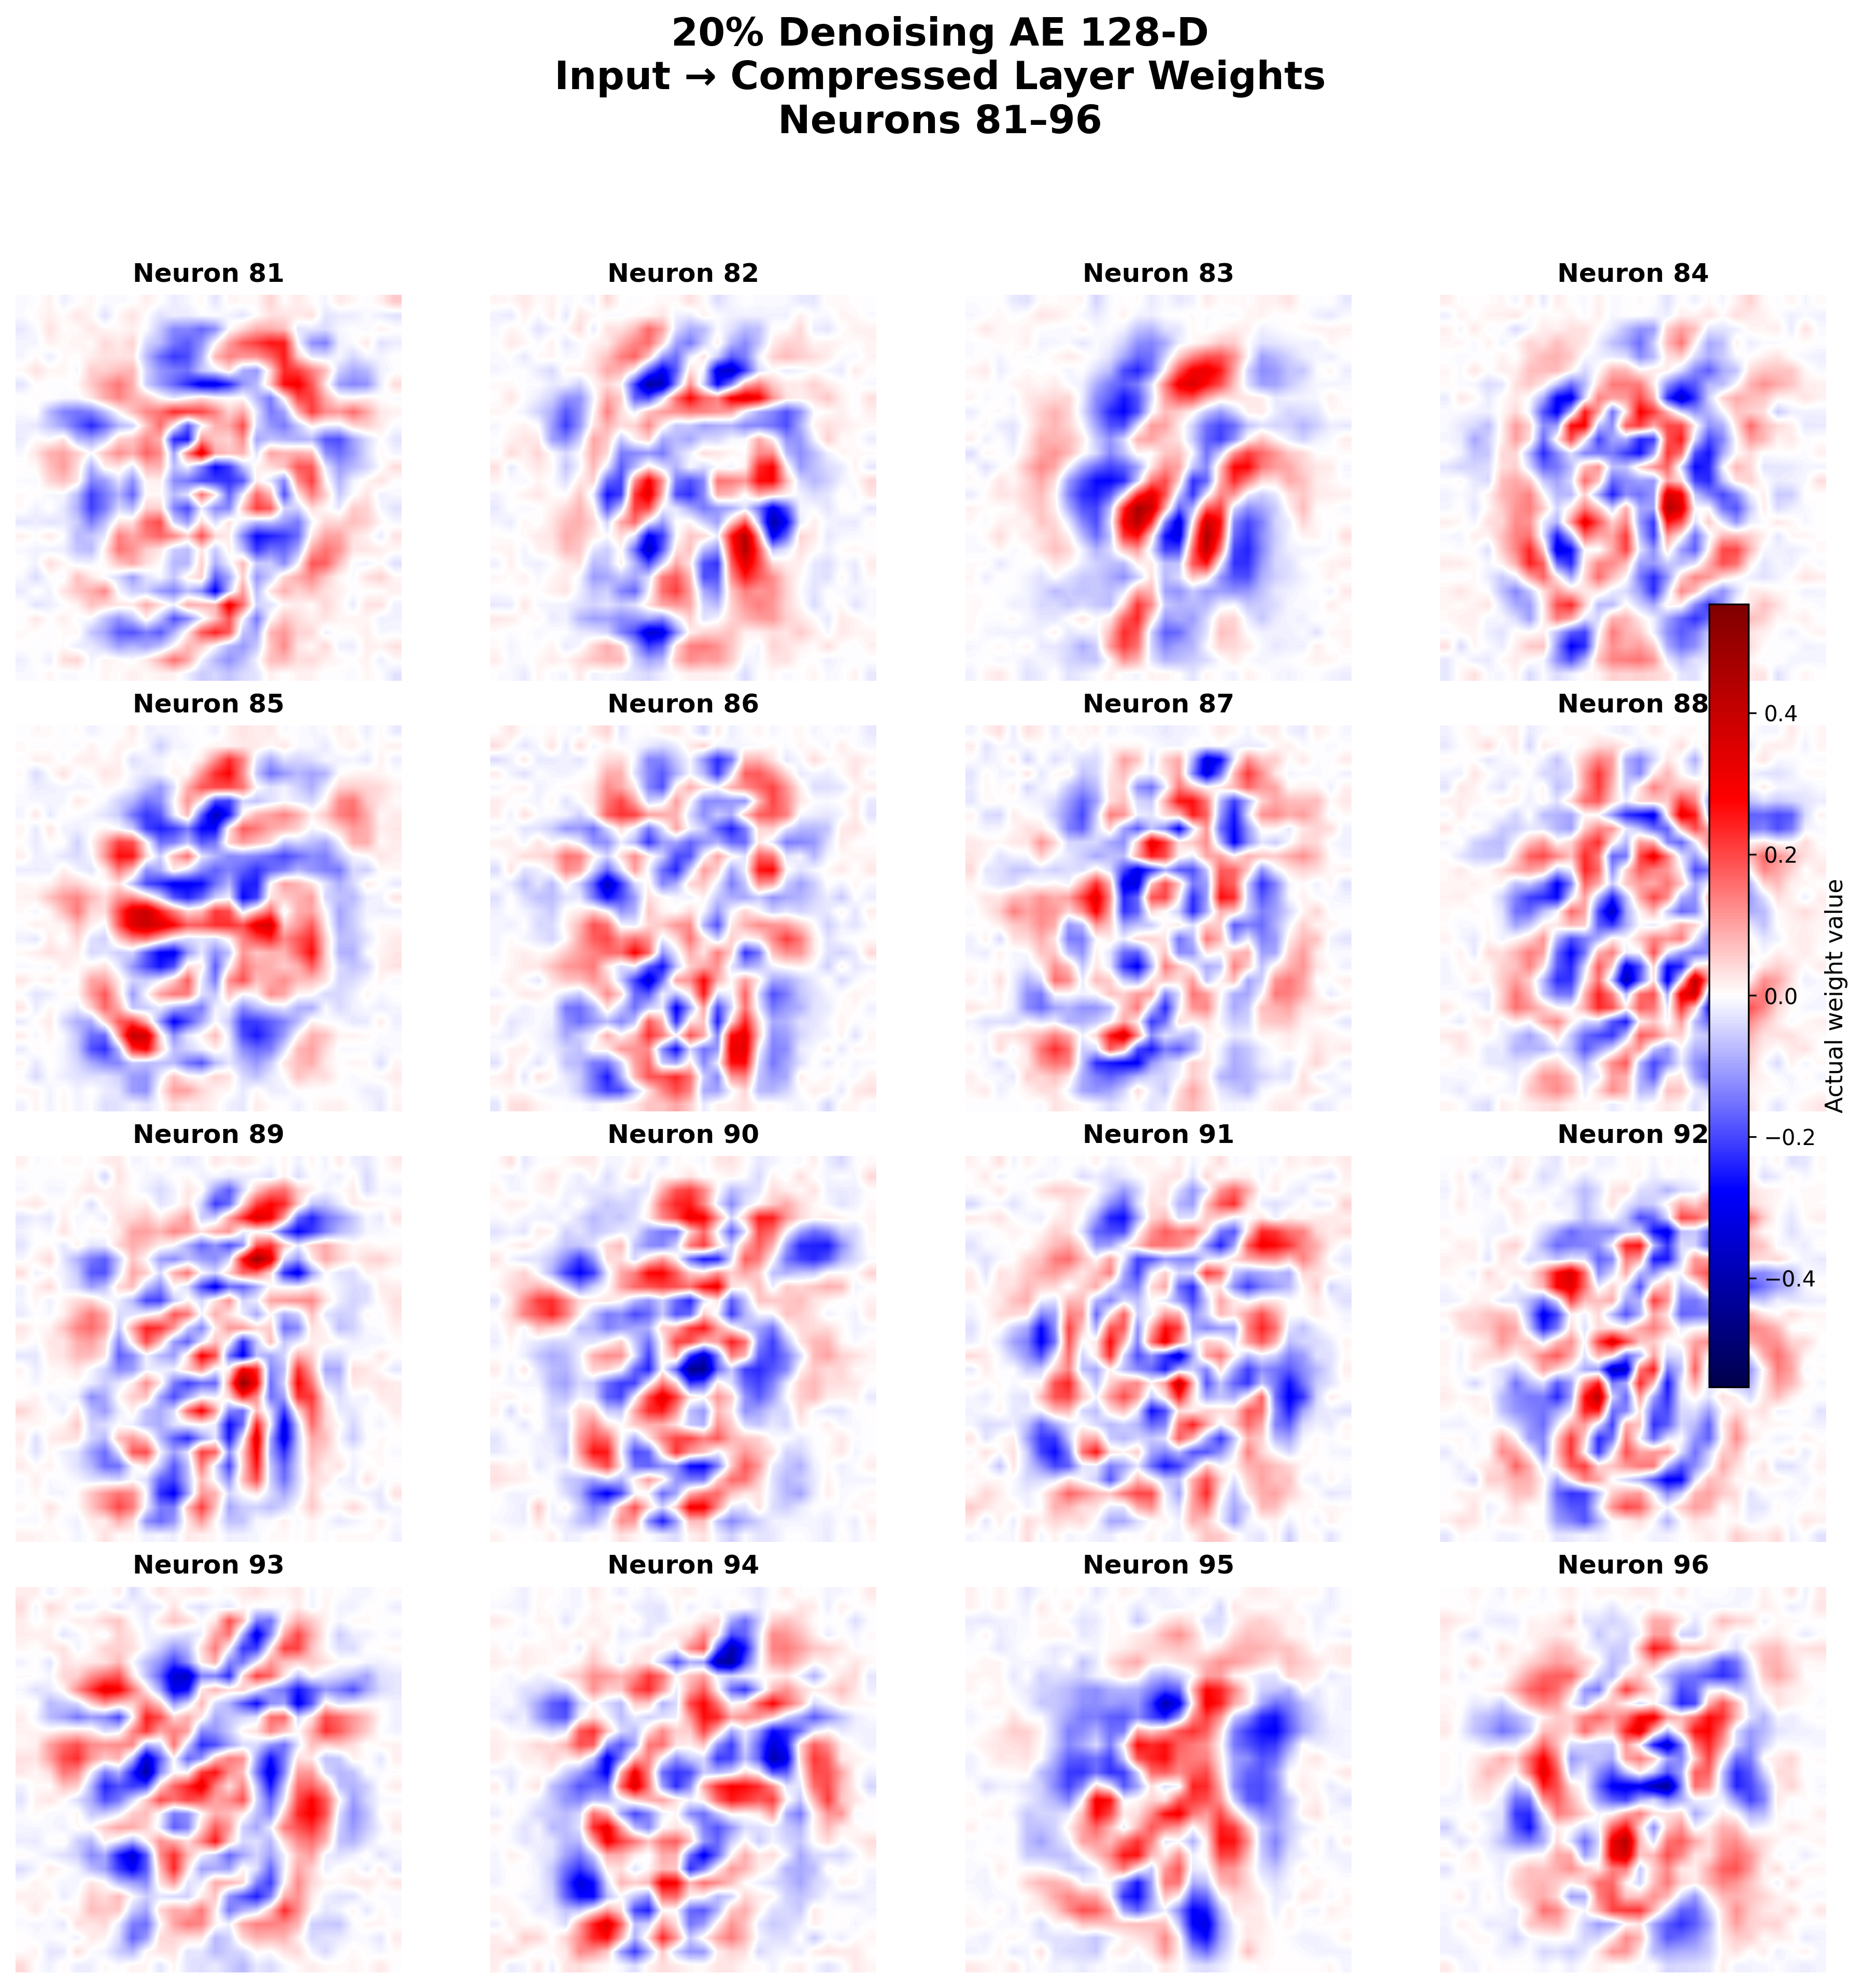
\includegraphics[width=0.99\linewidth,height=0.72\textheight,keepaspectratio]{figures/task6/20_pct_dae/neurons_081_096.png}
\caption{Input-to-bottleneck weight visualization for neurons 81--96.}
\label{fig:task6_14}
\end{figure}

\begin{figure}[H]
\centering
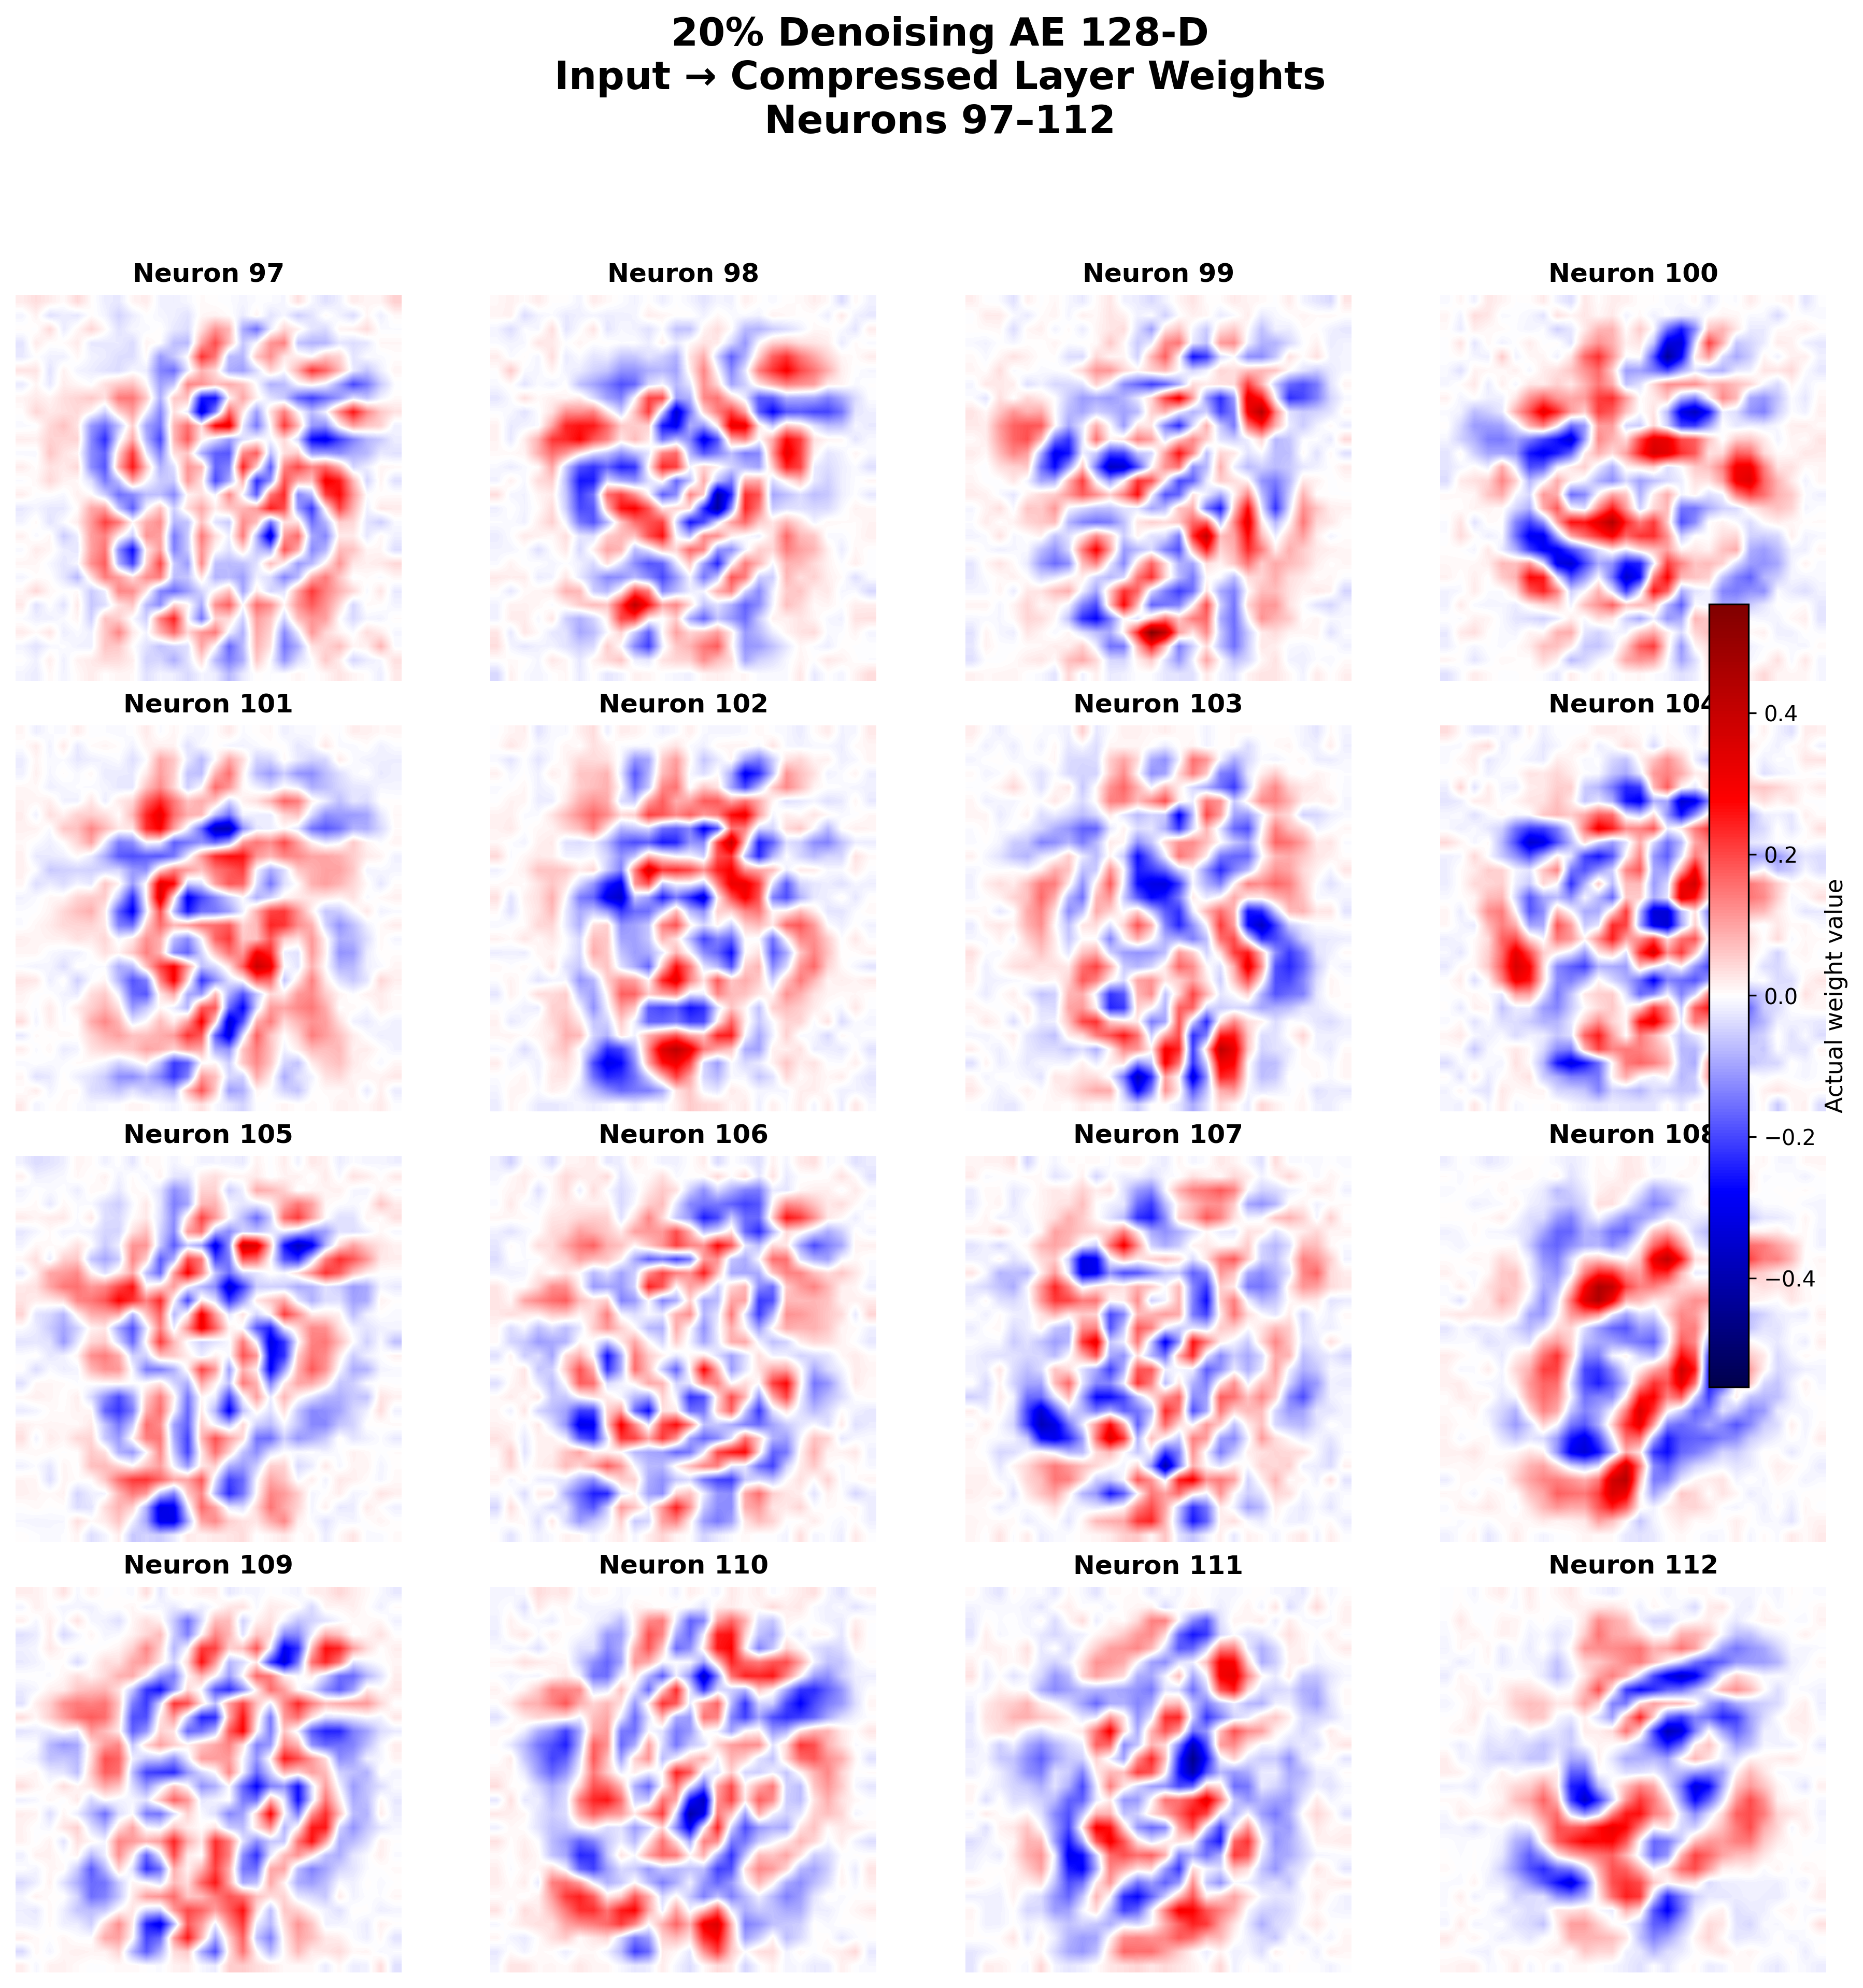
\includegraphics[width=0.99\linewidth,height=0.72\textheight,keepaspectratio]{figures/task6/20_pct_dae/neurons_097_112.png}
\caption{Input-to-bottleneck weight visualization for neurons 97--112.}
\label{fig:task6_15}
\end{figure}

\begin{figure}[H]
\centering
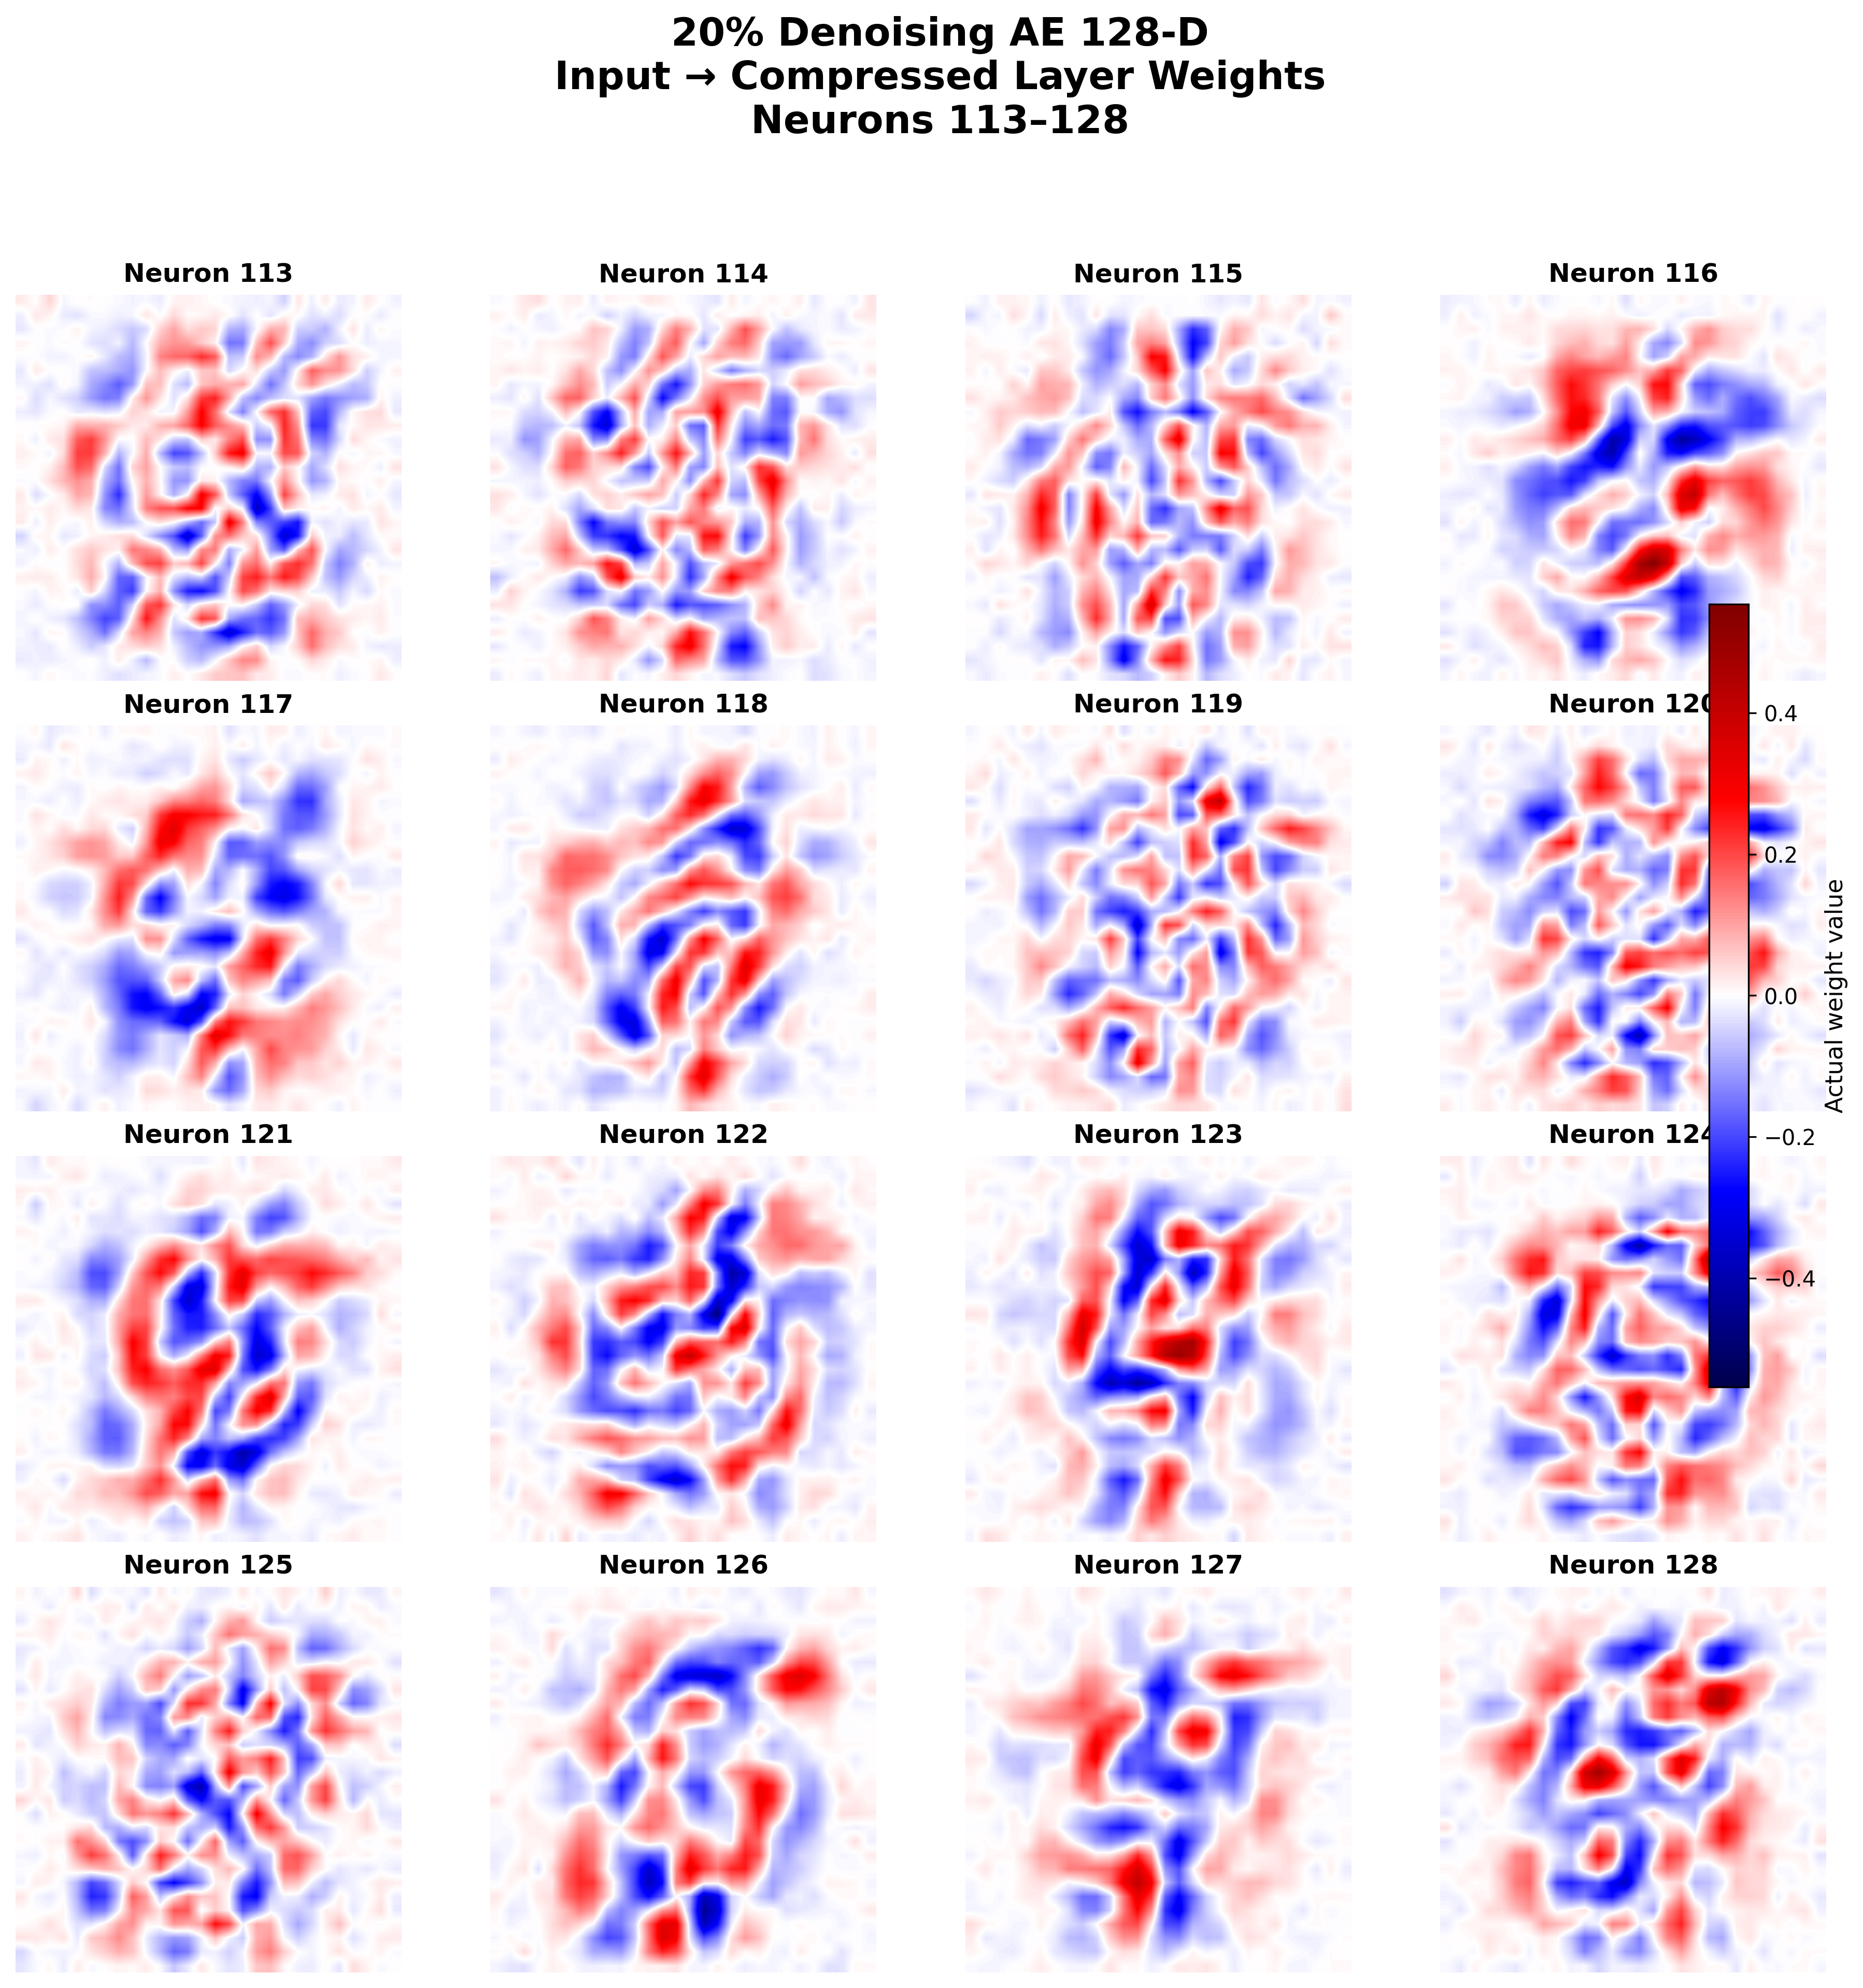
\includegraphics[width=0.99\linewidth,height=0.72\textheight,keepaspectratio]{figures/task6/20_pct_dae/neurons_113_128.png}
\caption{Input-to-bottleneck weight visualization for neurons 113--128.}
\label{fig:task6_16}
\end{figure}

\begin{figure}[H]
\centering
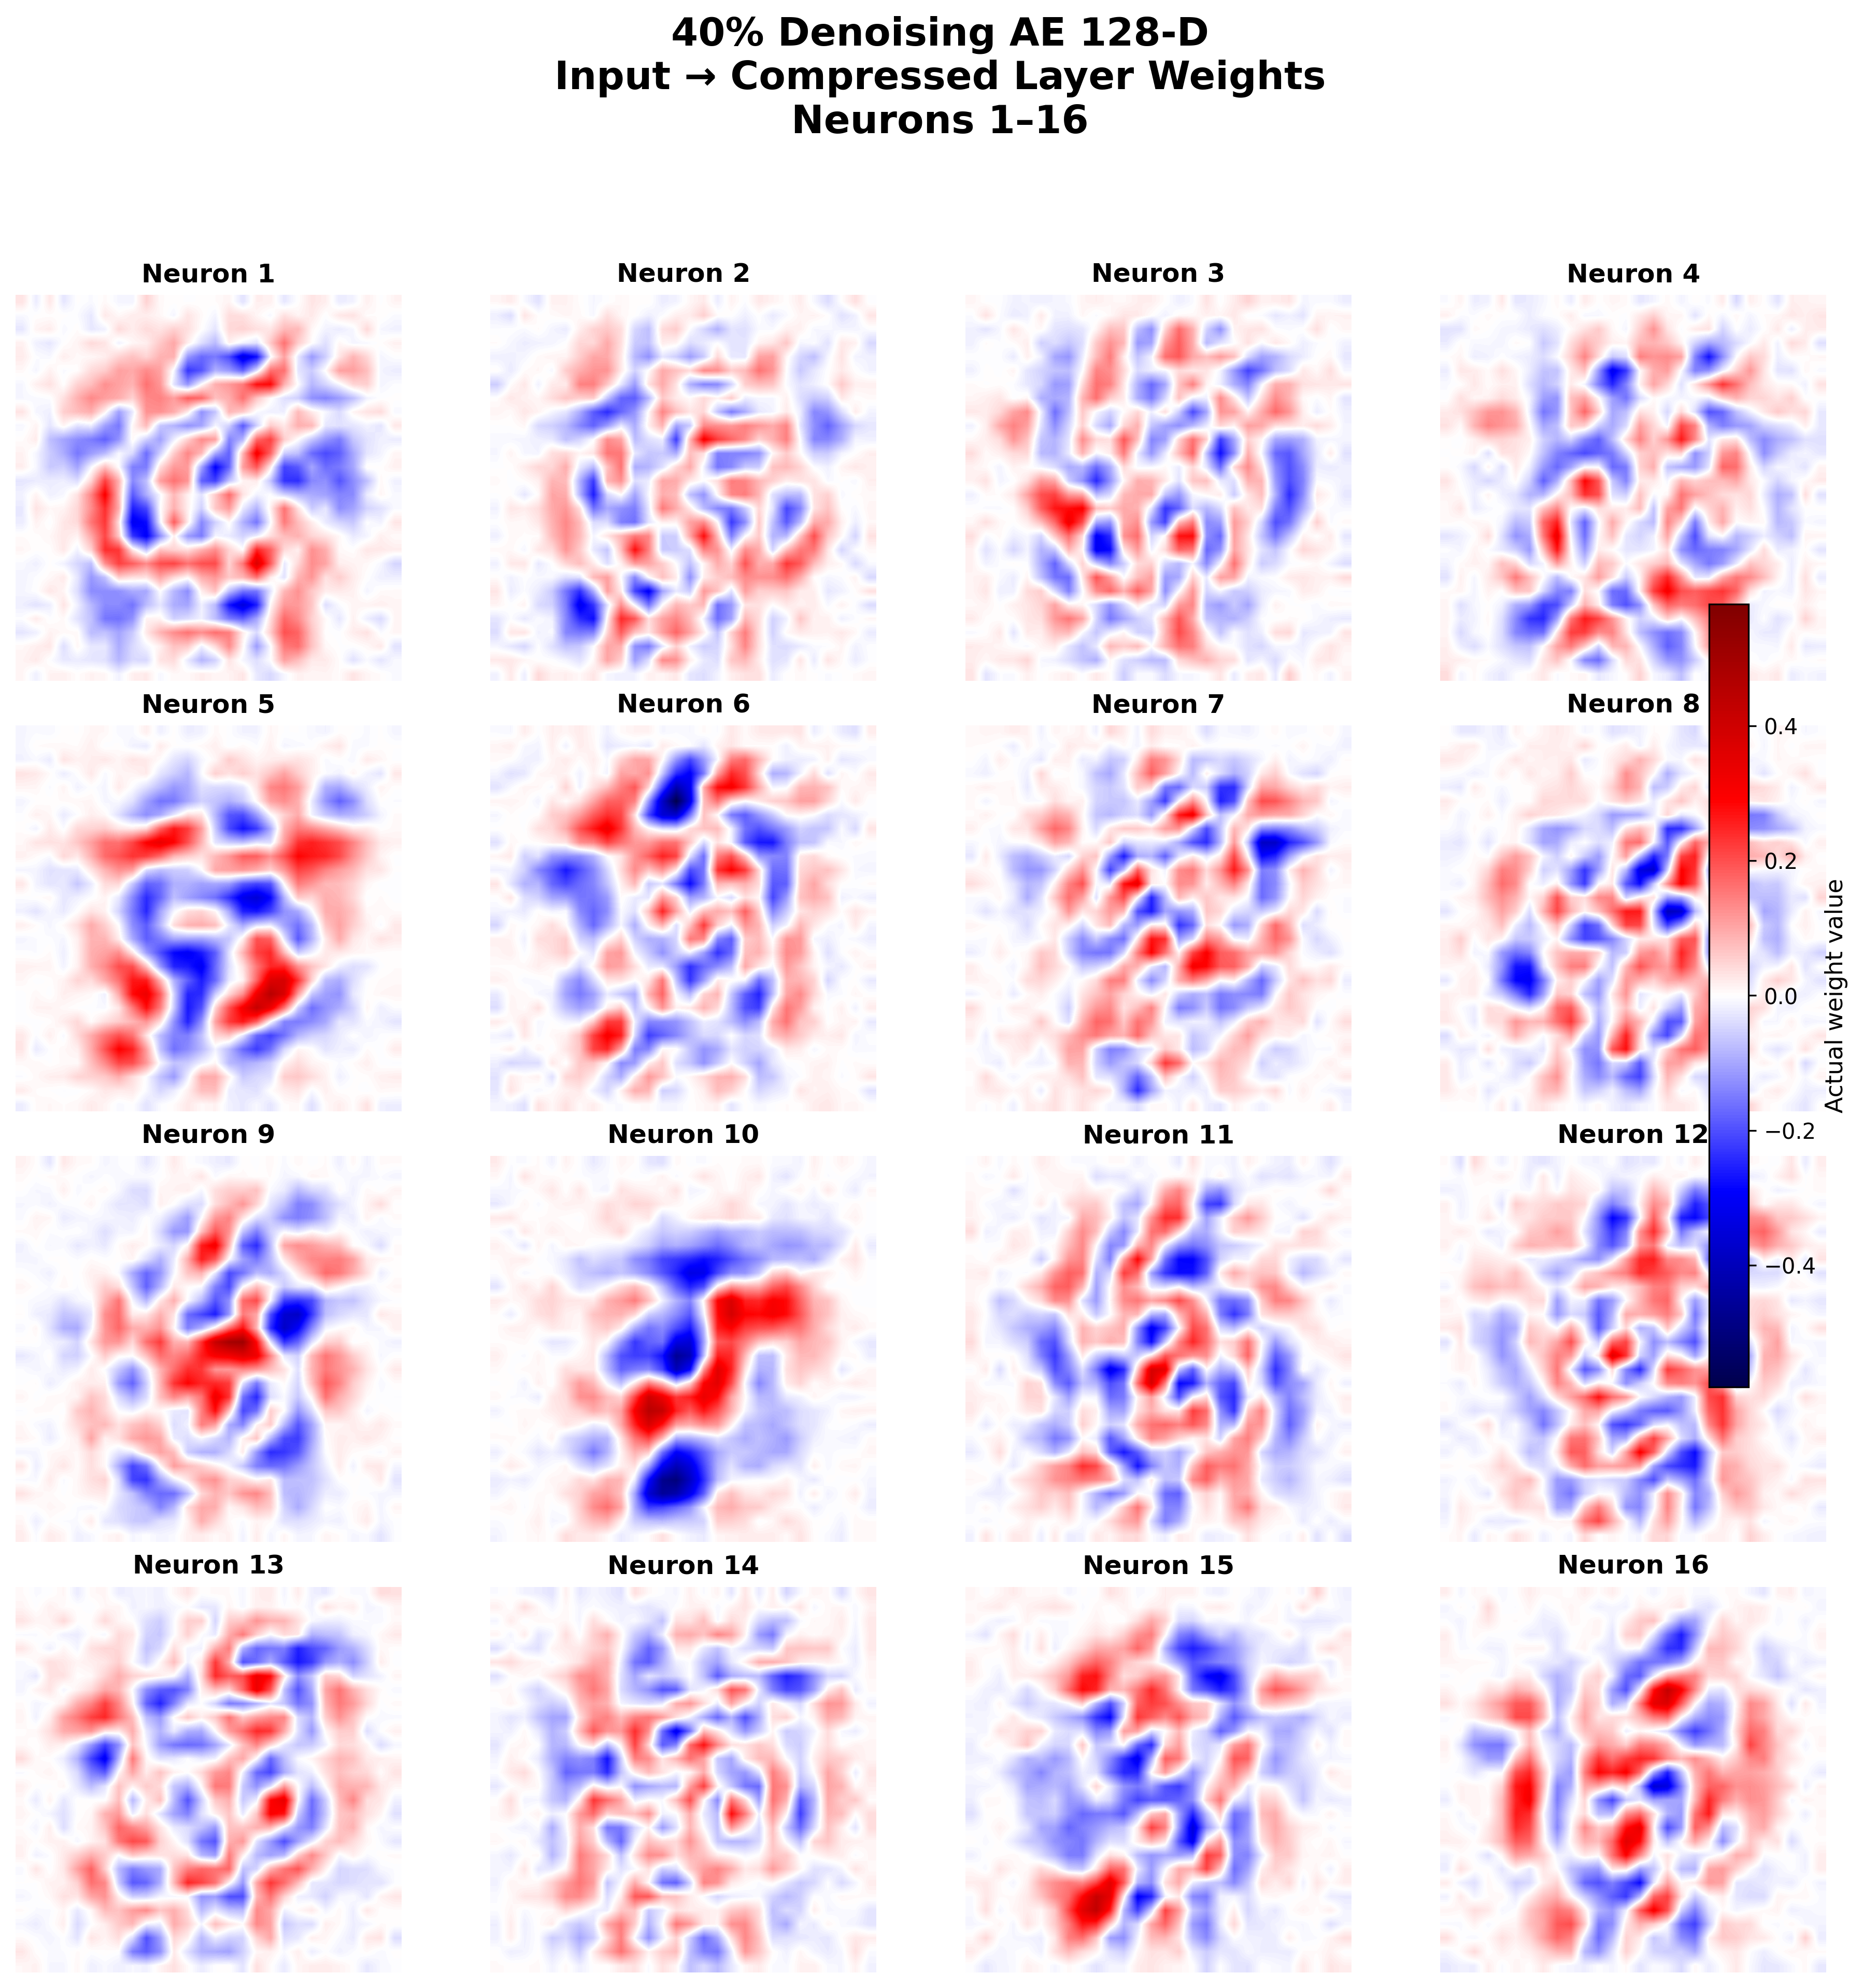
\includegraphics[width=0.99\linewidth,height=0.72\textheight,keepaspectratio]{figures/task6/40_pct_dae/neurons_001_016.png}
\caption{Input-to-bottleneck weight visualization for neurons 1--16.}
\label{fig:task6_17}
\end{figure}

\begin{figure}[H]
\centering
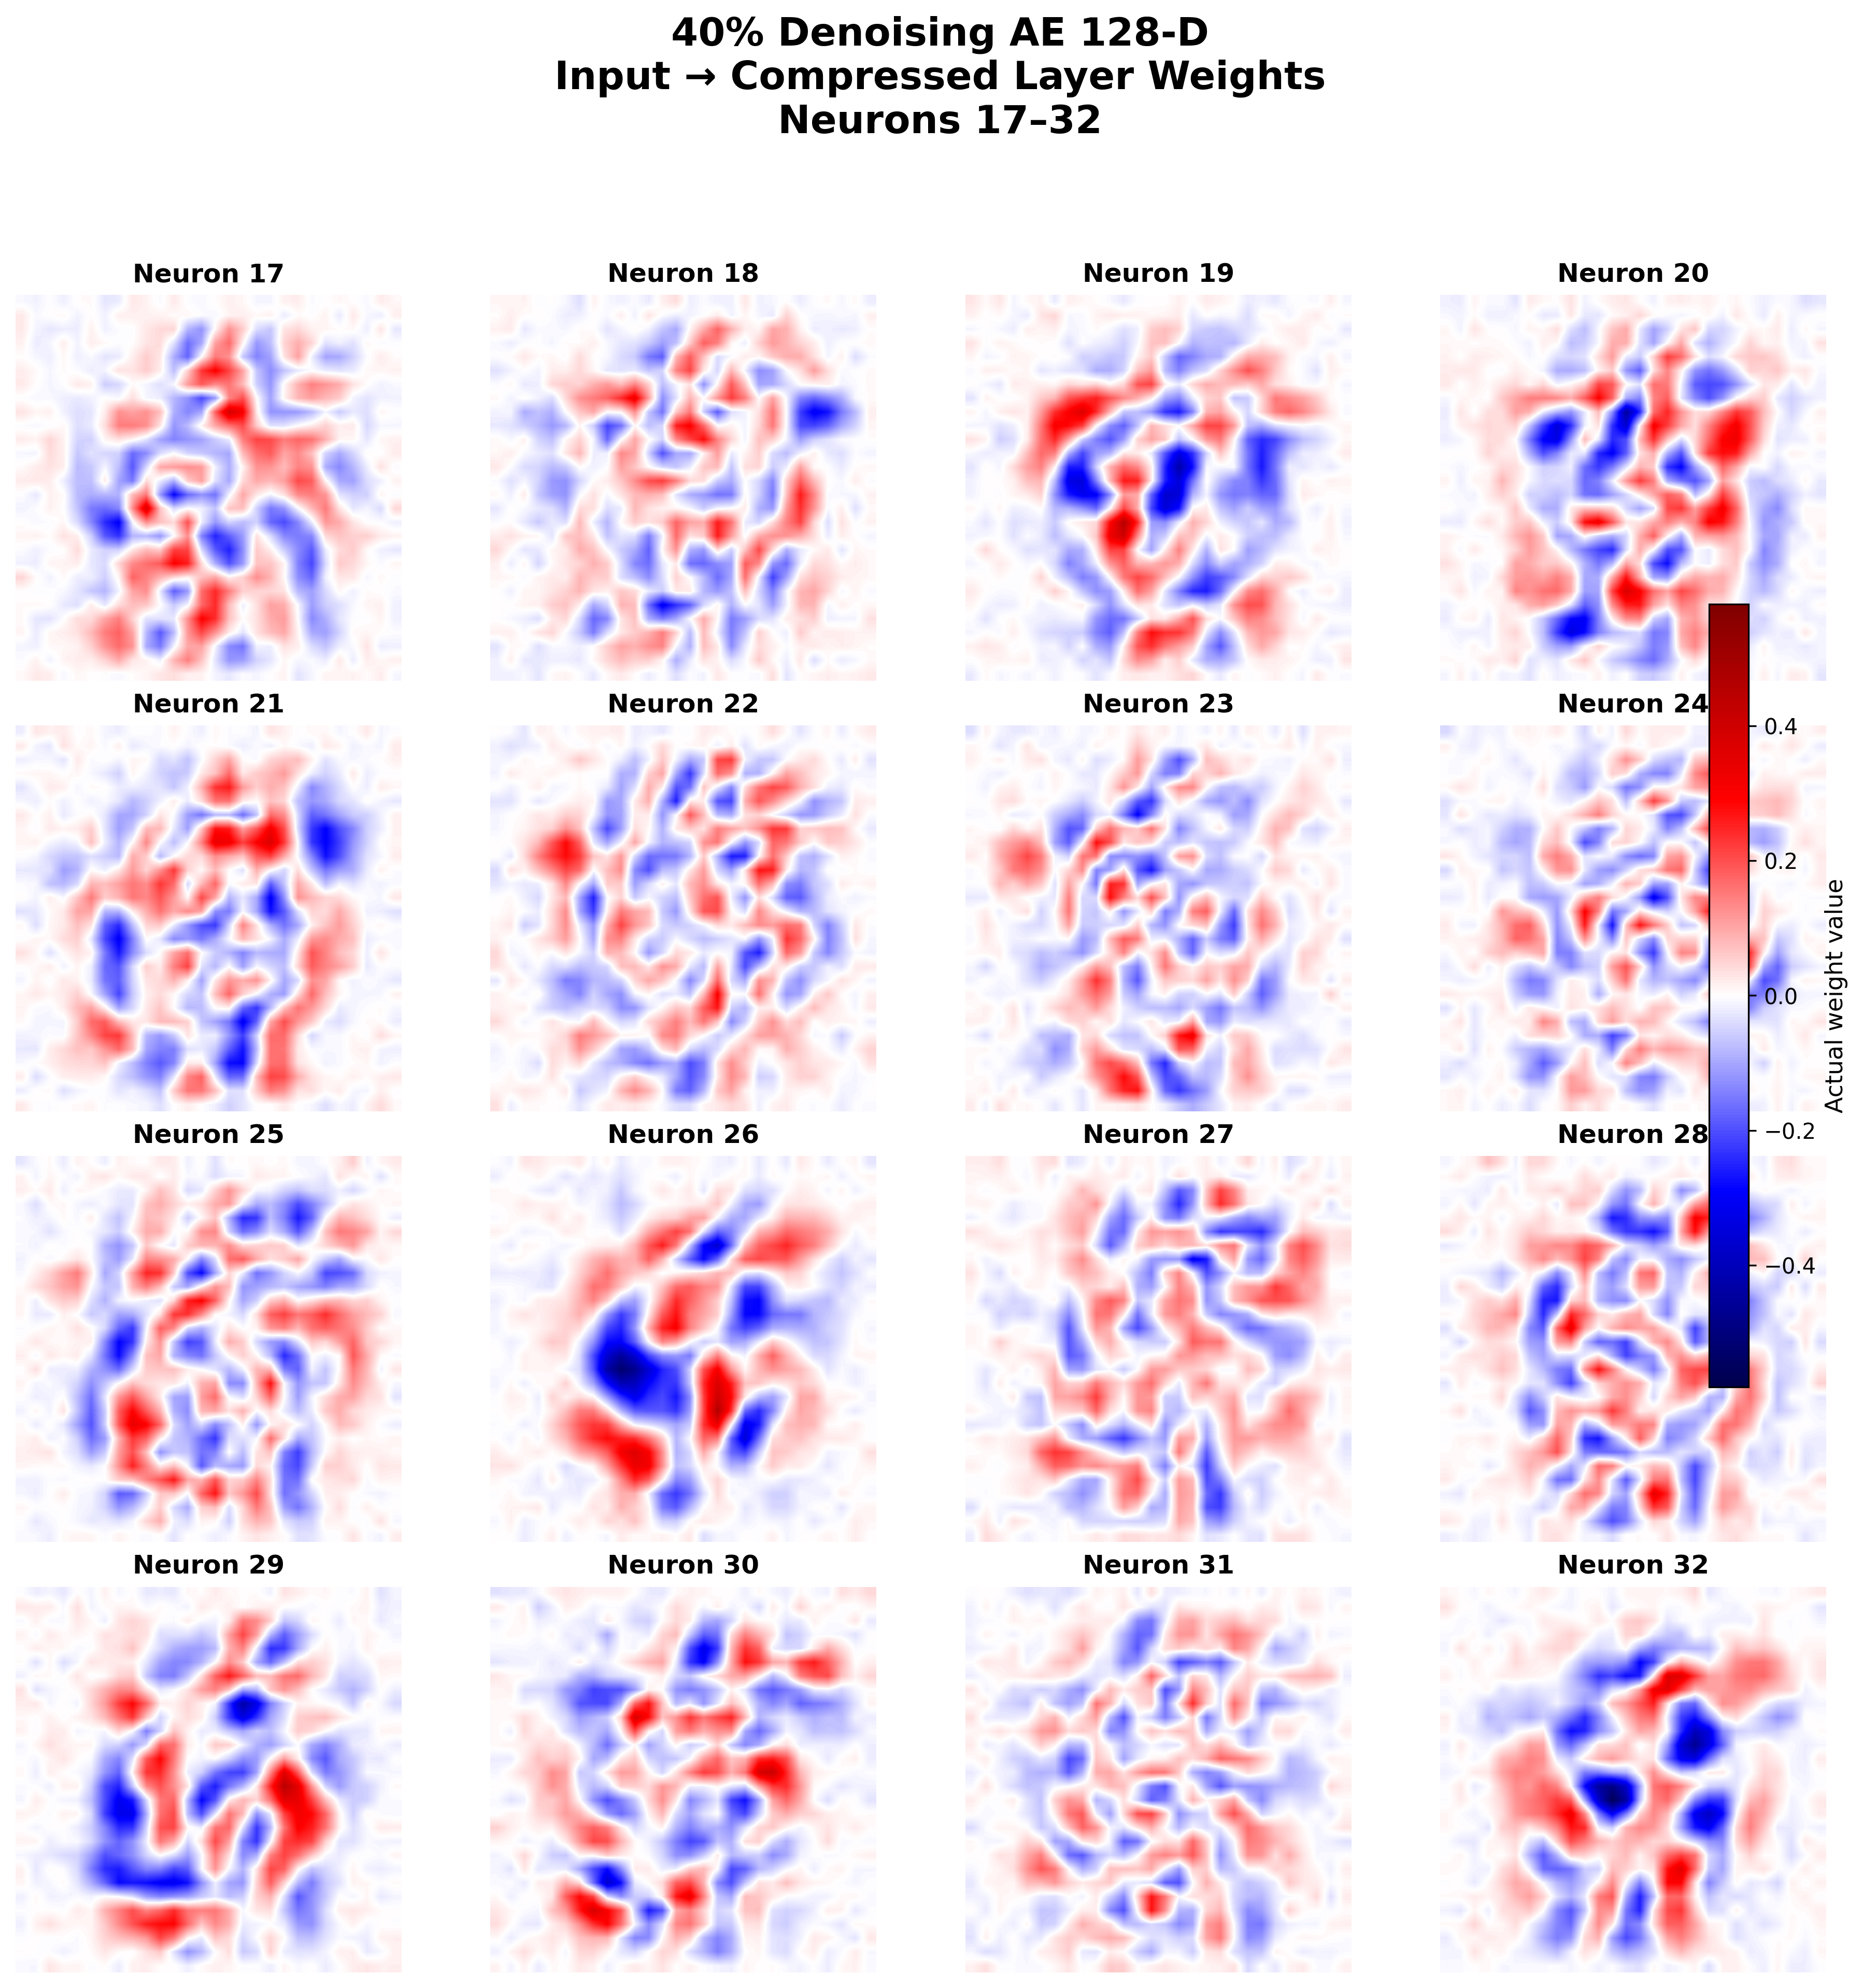
\includegraphics[width=0.99\linewidth,height=0.72\textheight,keepaspectratio]{figures/task6/40_pct_dae/neurons_017_032.png}
\caption{Input-to-bottleneck weight visualization for neurons 17--32.}
\label{fig:task6_18}
\end{figure}

\begin{figure}[H]
\centering
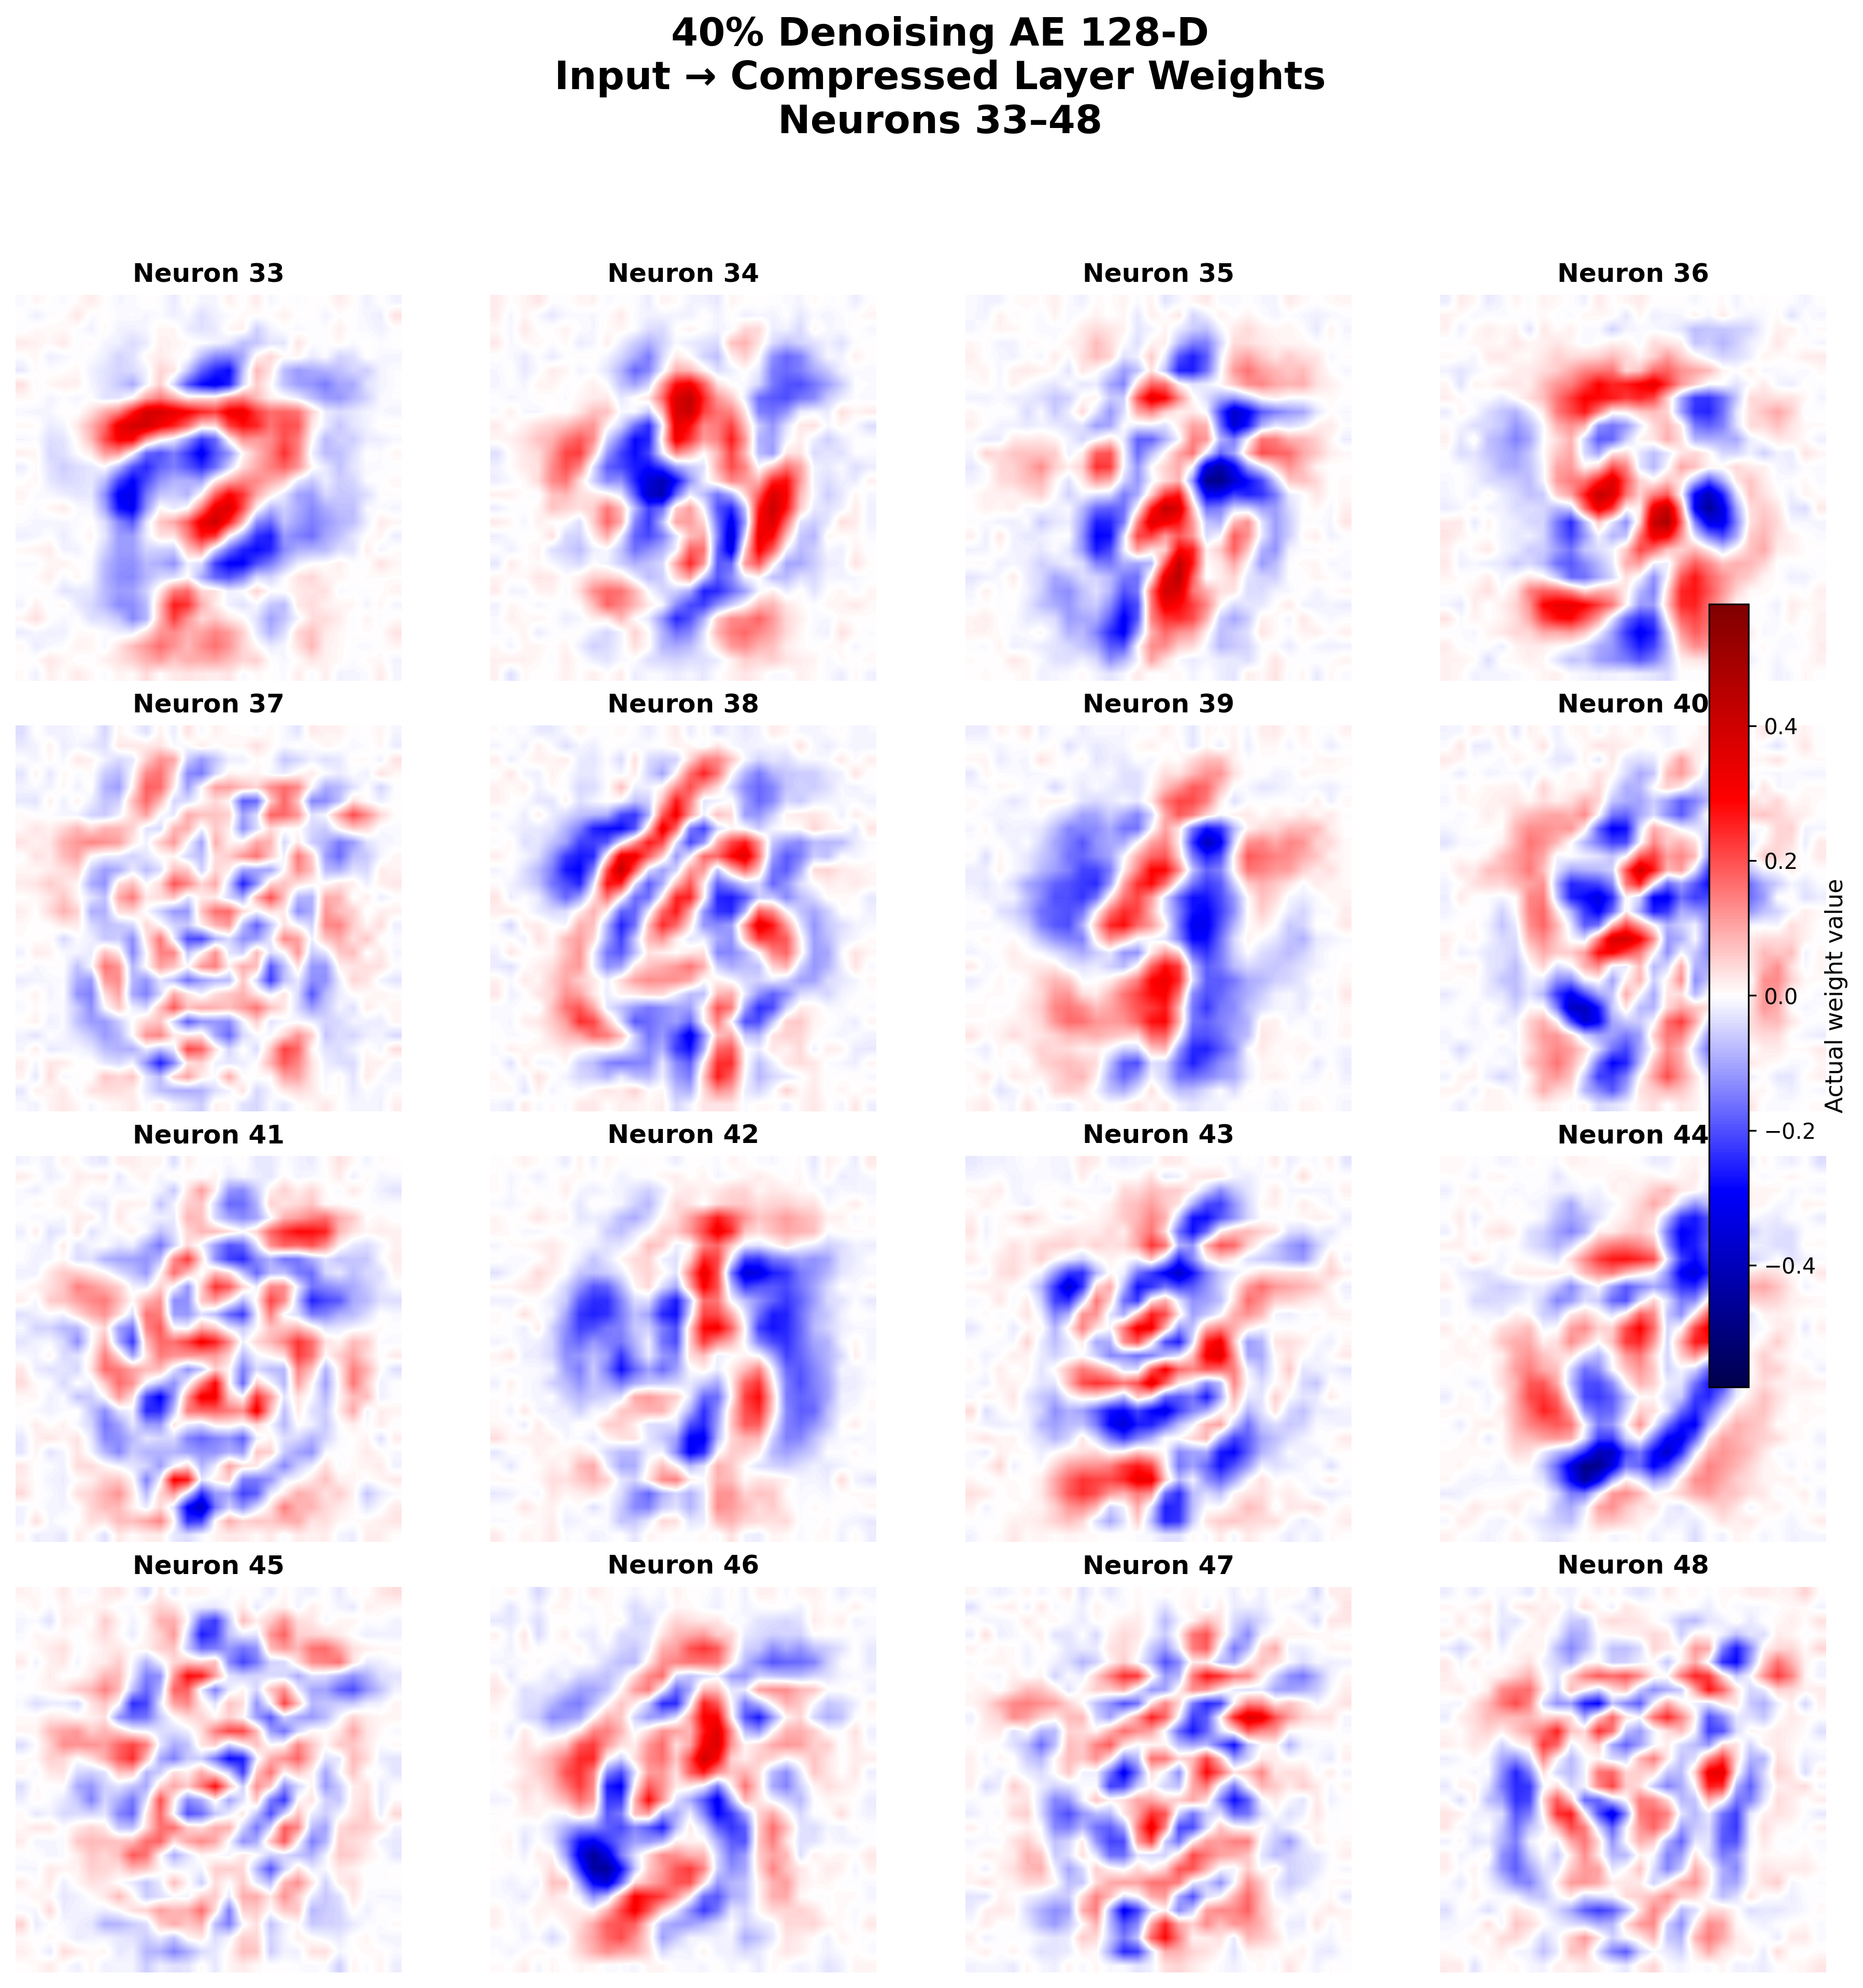
\includegraphics[width=0.99\linewidth,height=0.72\textheight,keepaspectratio]{figures/task6/40_pct_dae/neurons_033_048.png}
\caption{Input-to-bottleneck weight visualization for neurons 33--48.}
\label{fig:task6_19}
\end{figure}

\begin{figure}[H]
\centering
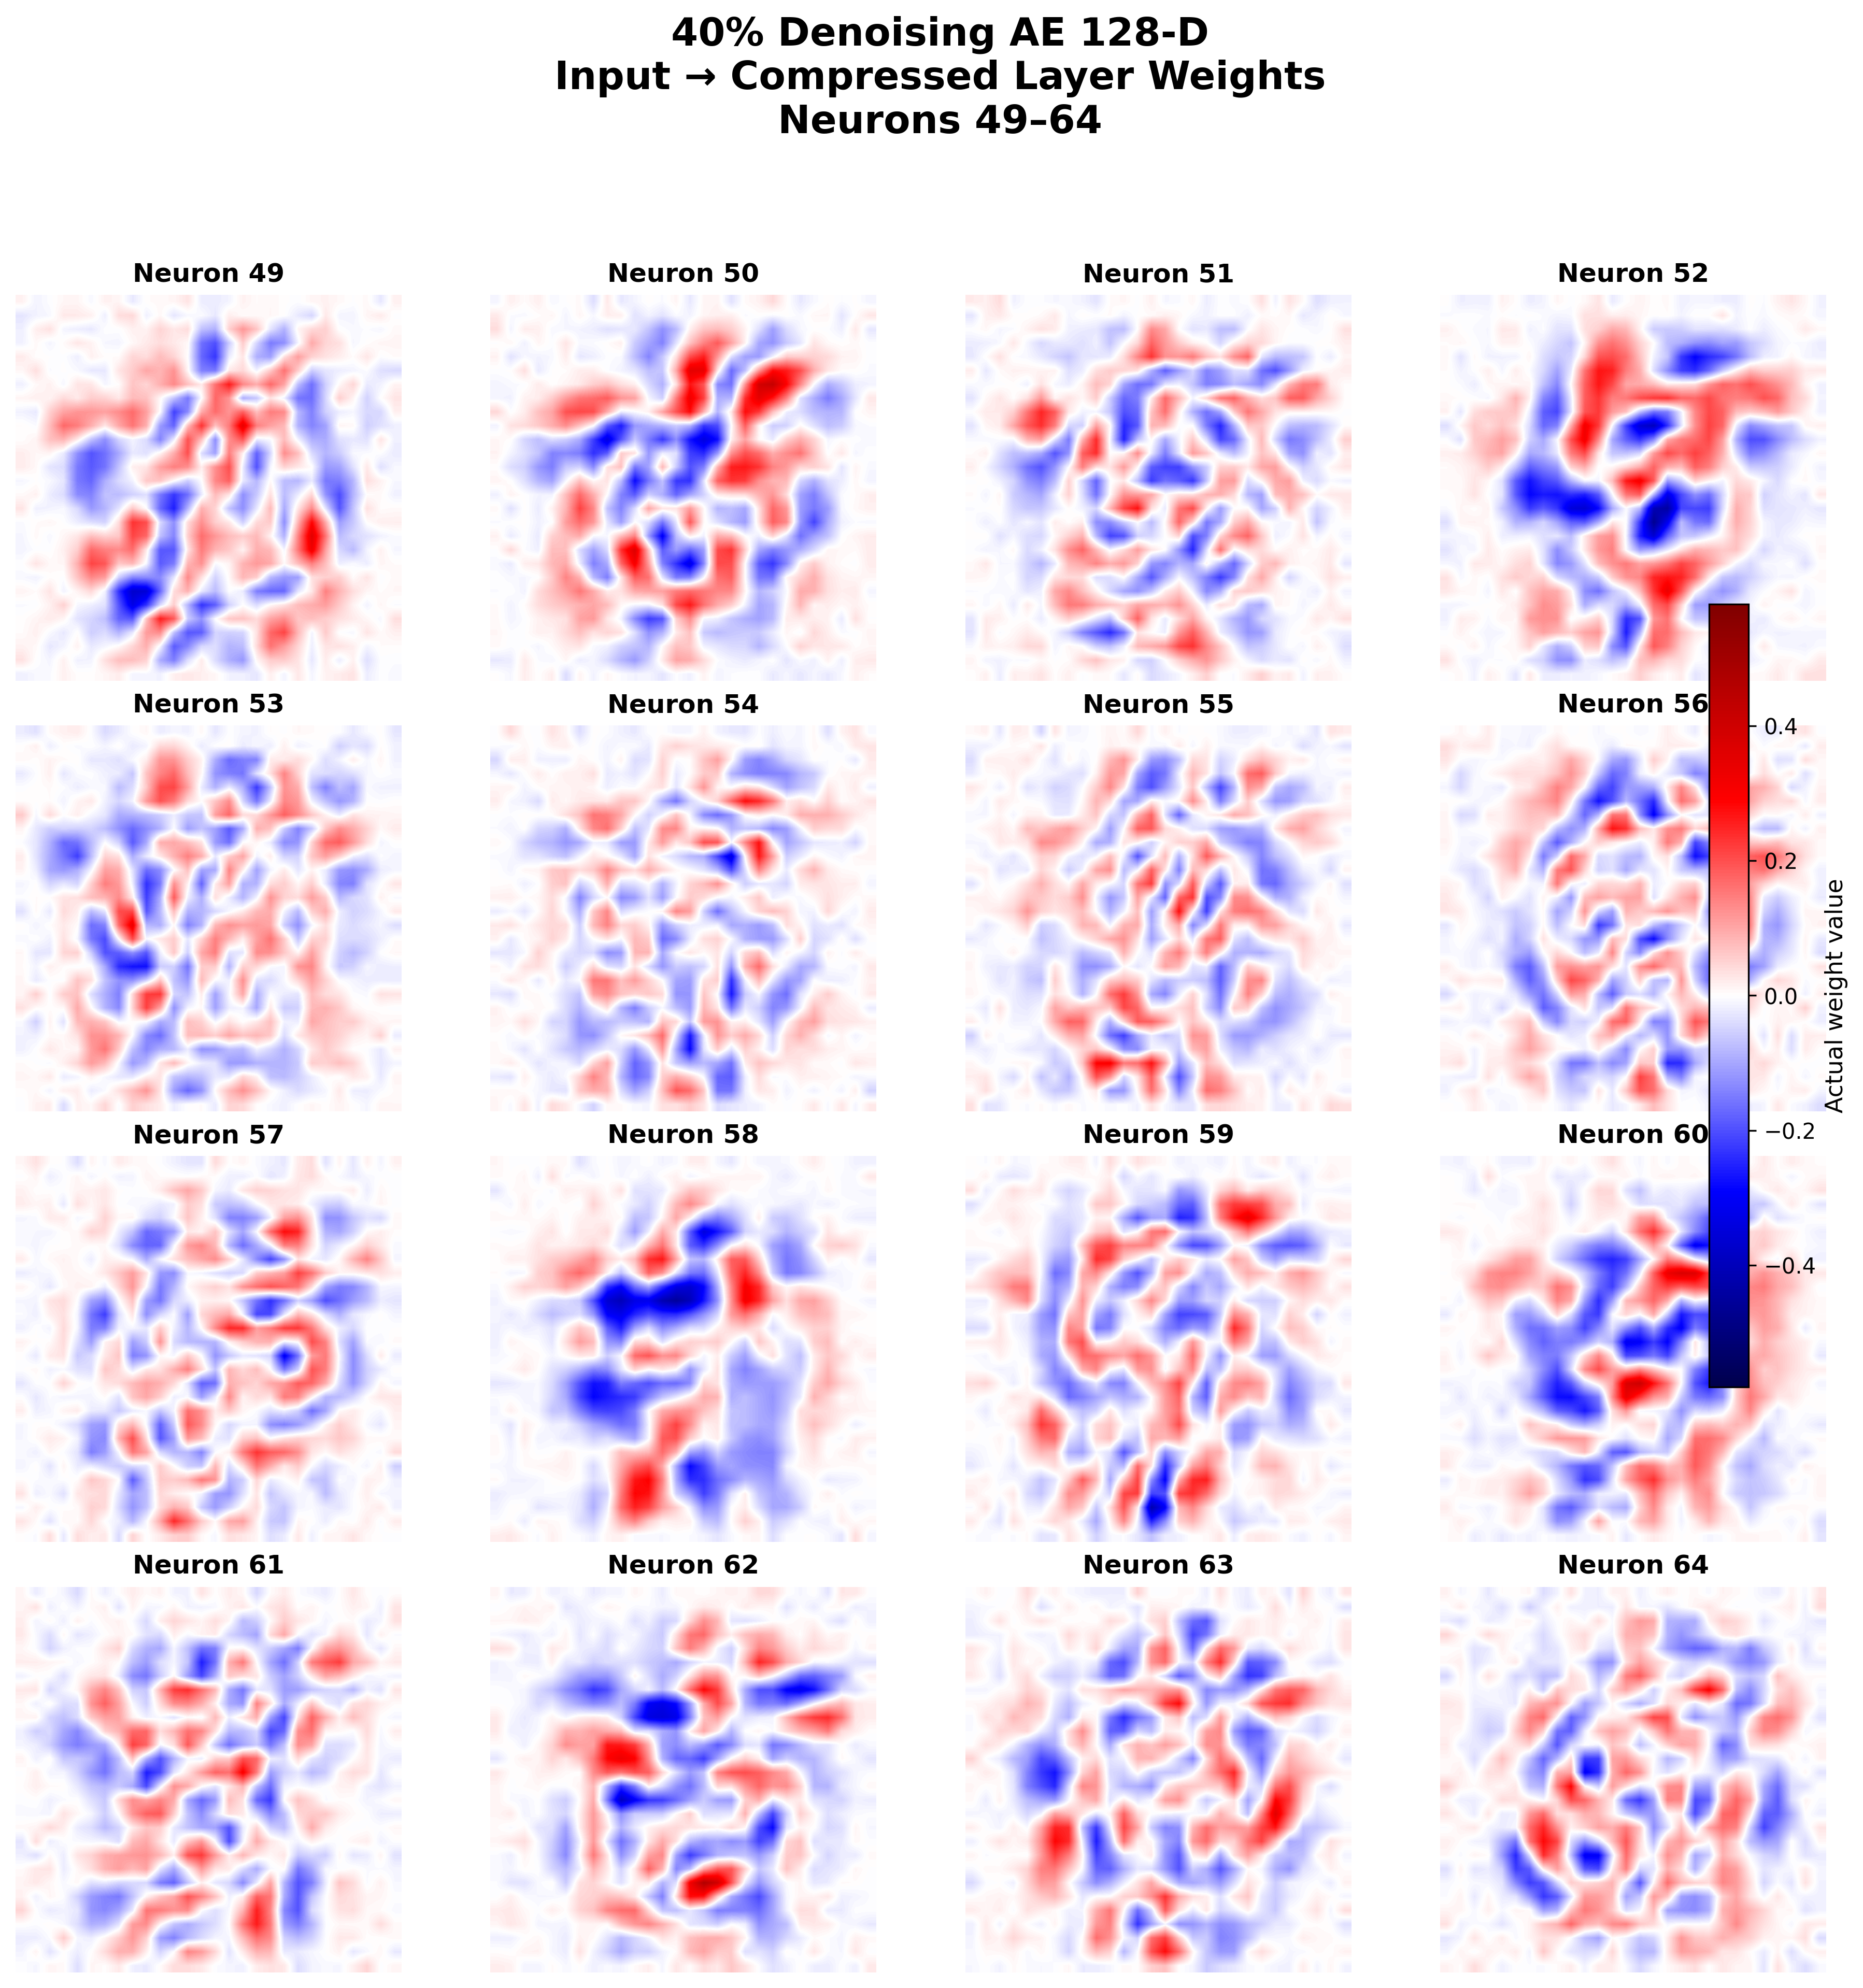
\includegraphics[width=0.99\linewidth,height=0.72\textheight,keepaspectratio]{figures/task6/40_pct_dae/neurons_049_064.png}
\caption{Input-to-bottleneck weight visualization for neurons 49--64.}
\label{fig:task6_20}
\end{figure}

\begin{figure}[H]
\centering
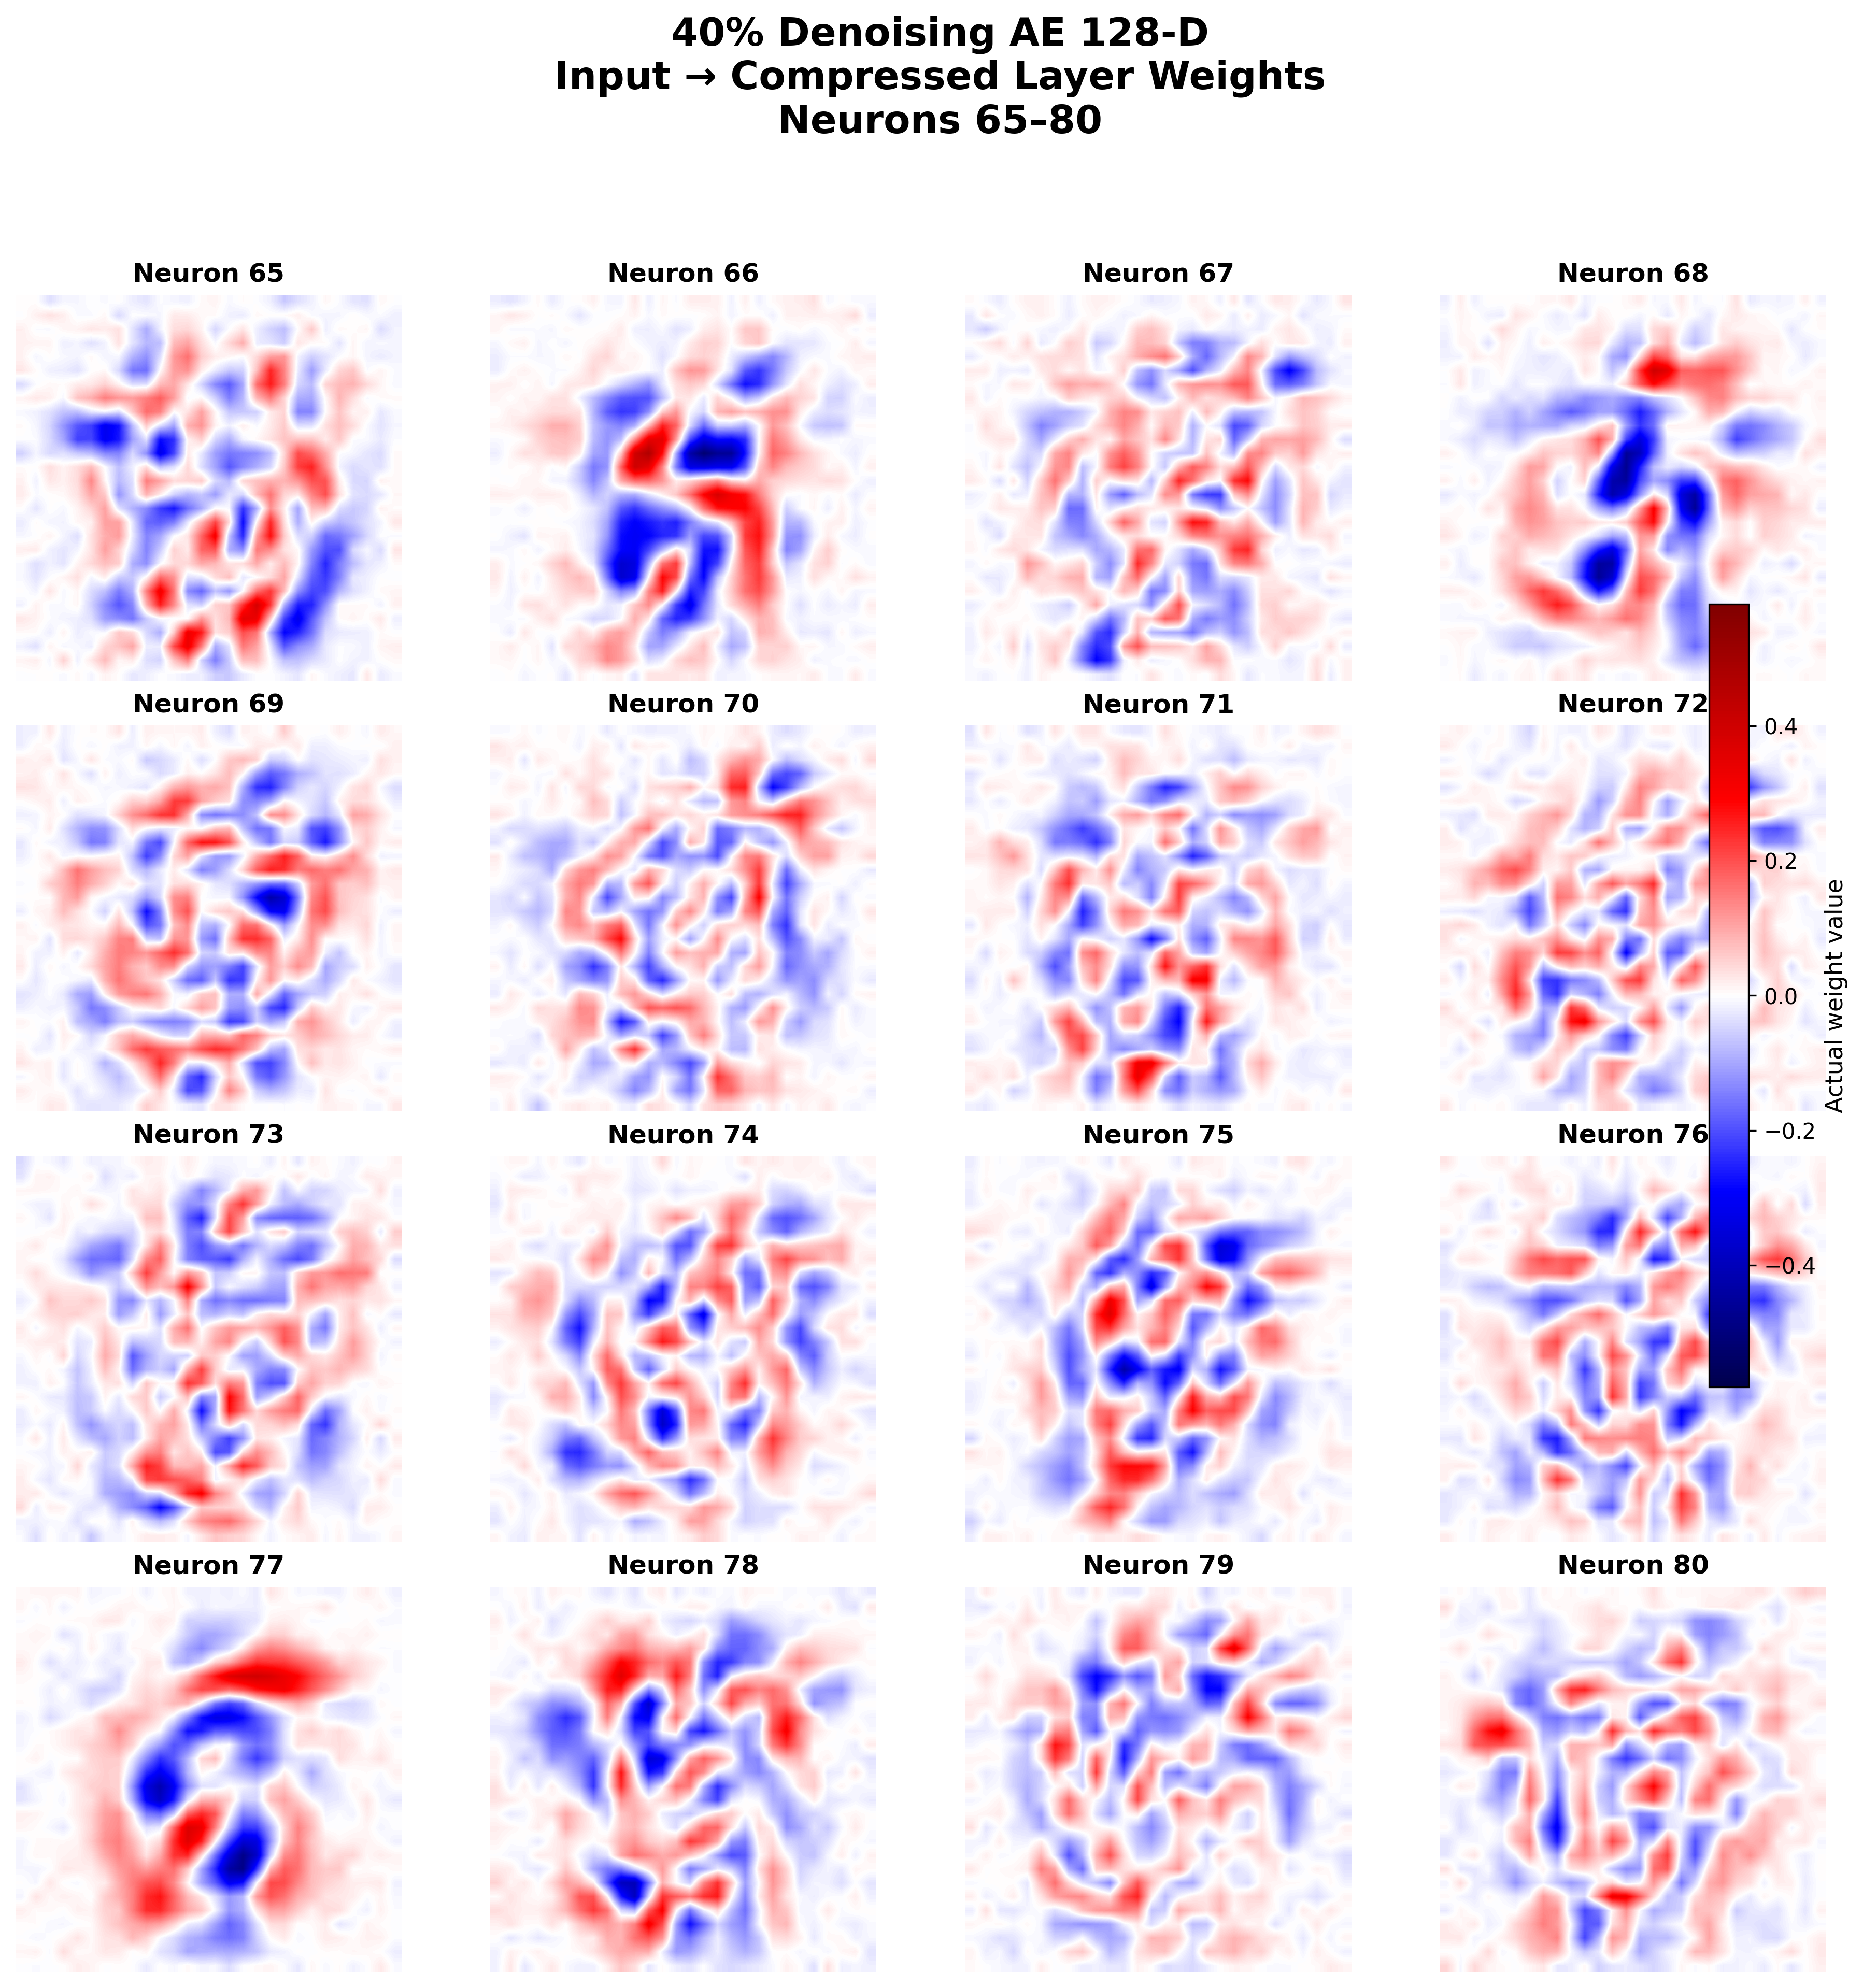
\includegraphics[width=0.99\linewidth,height=0.72\textheight,keepaspectratio]{figures/task6/40_pct_dae/neurons_065_080.png}
\caption{Input-to-bottleneck weight visualization for neurons 65--80.}
\label{fig:task6_21}
\end{figure}

\begin{figure}[H]
\centering
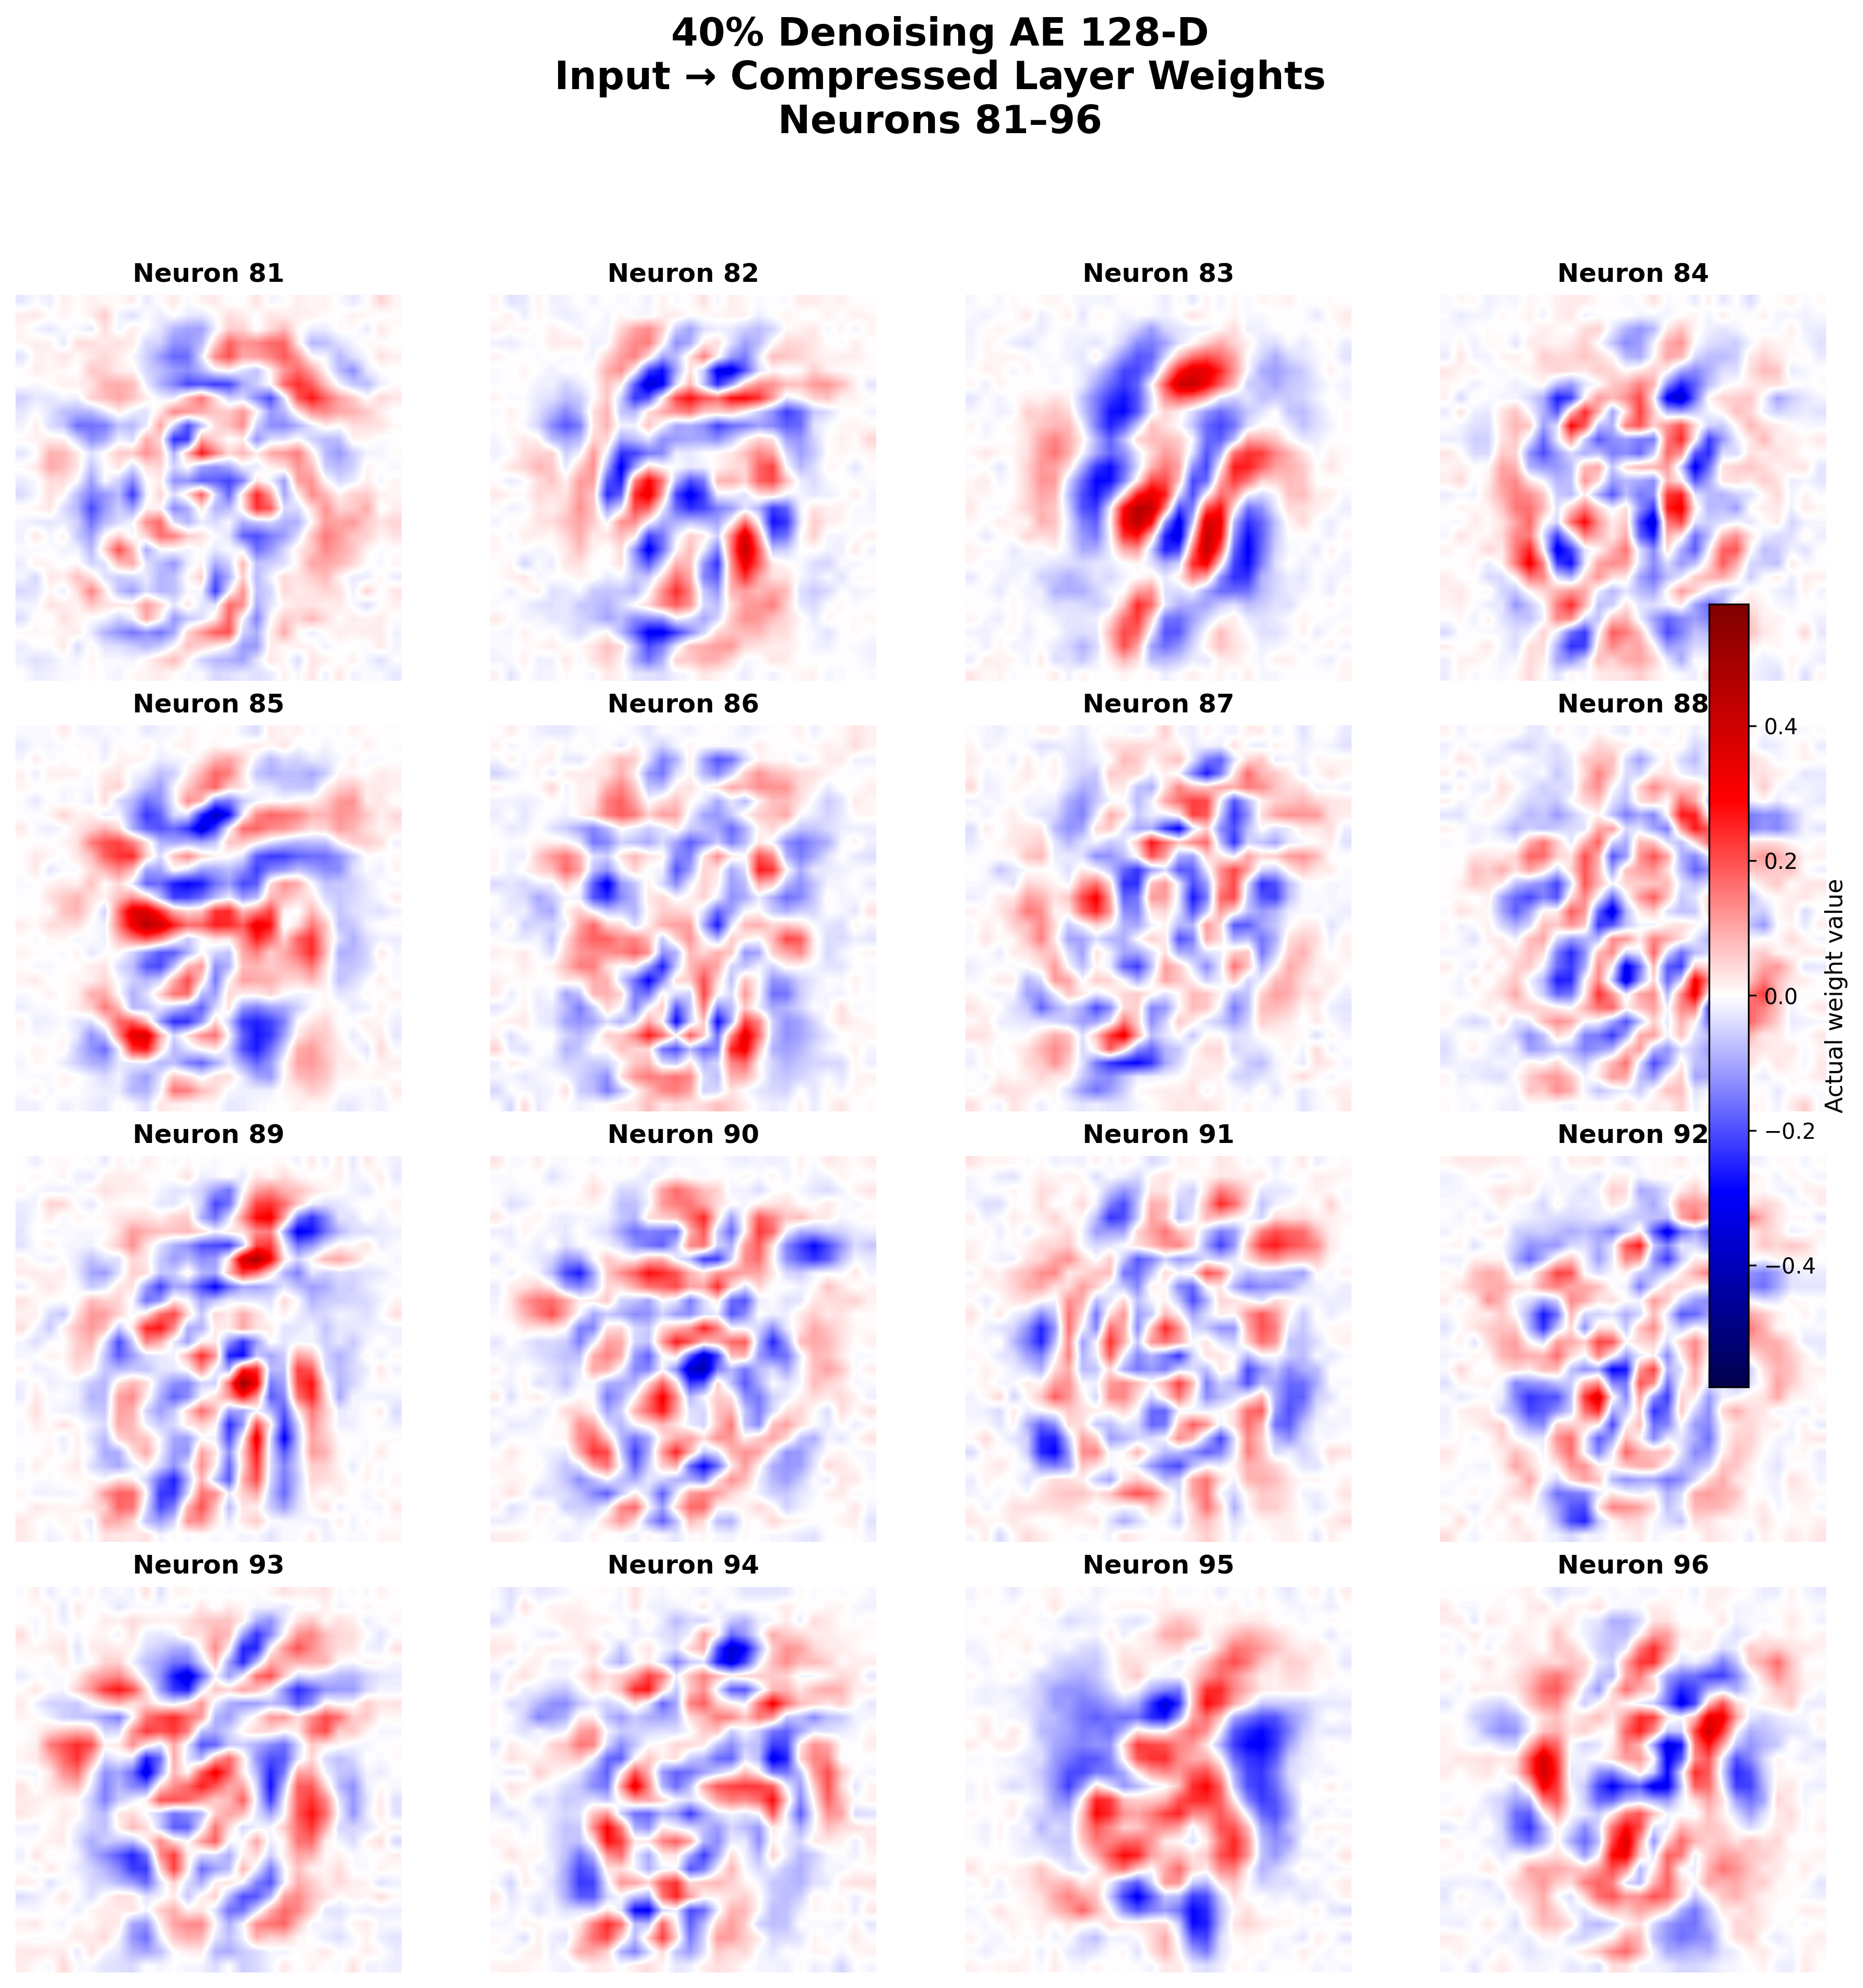
\includegraphics[width=0.99\linewidth,height=0.72\textheight,keepaspectratio]{figures/task6/40_pct_dae/neurons_081_096.png}
\caption{Input-to-bottleneck weight visualization for neurons 81--96.}
\label{fig:task6_22}
\end{figure}

\begin{figure}[H]
\centering
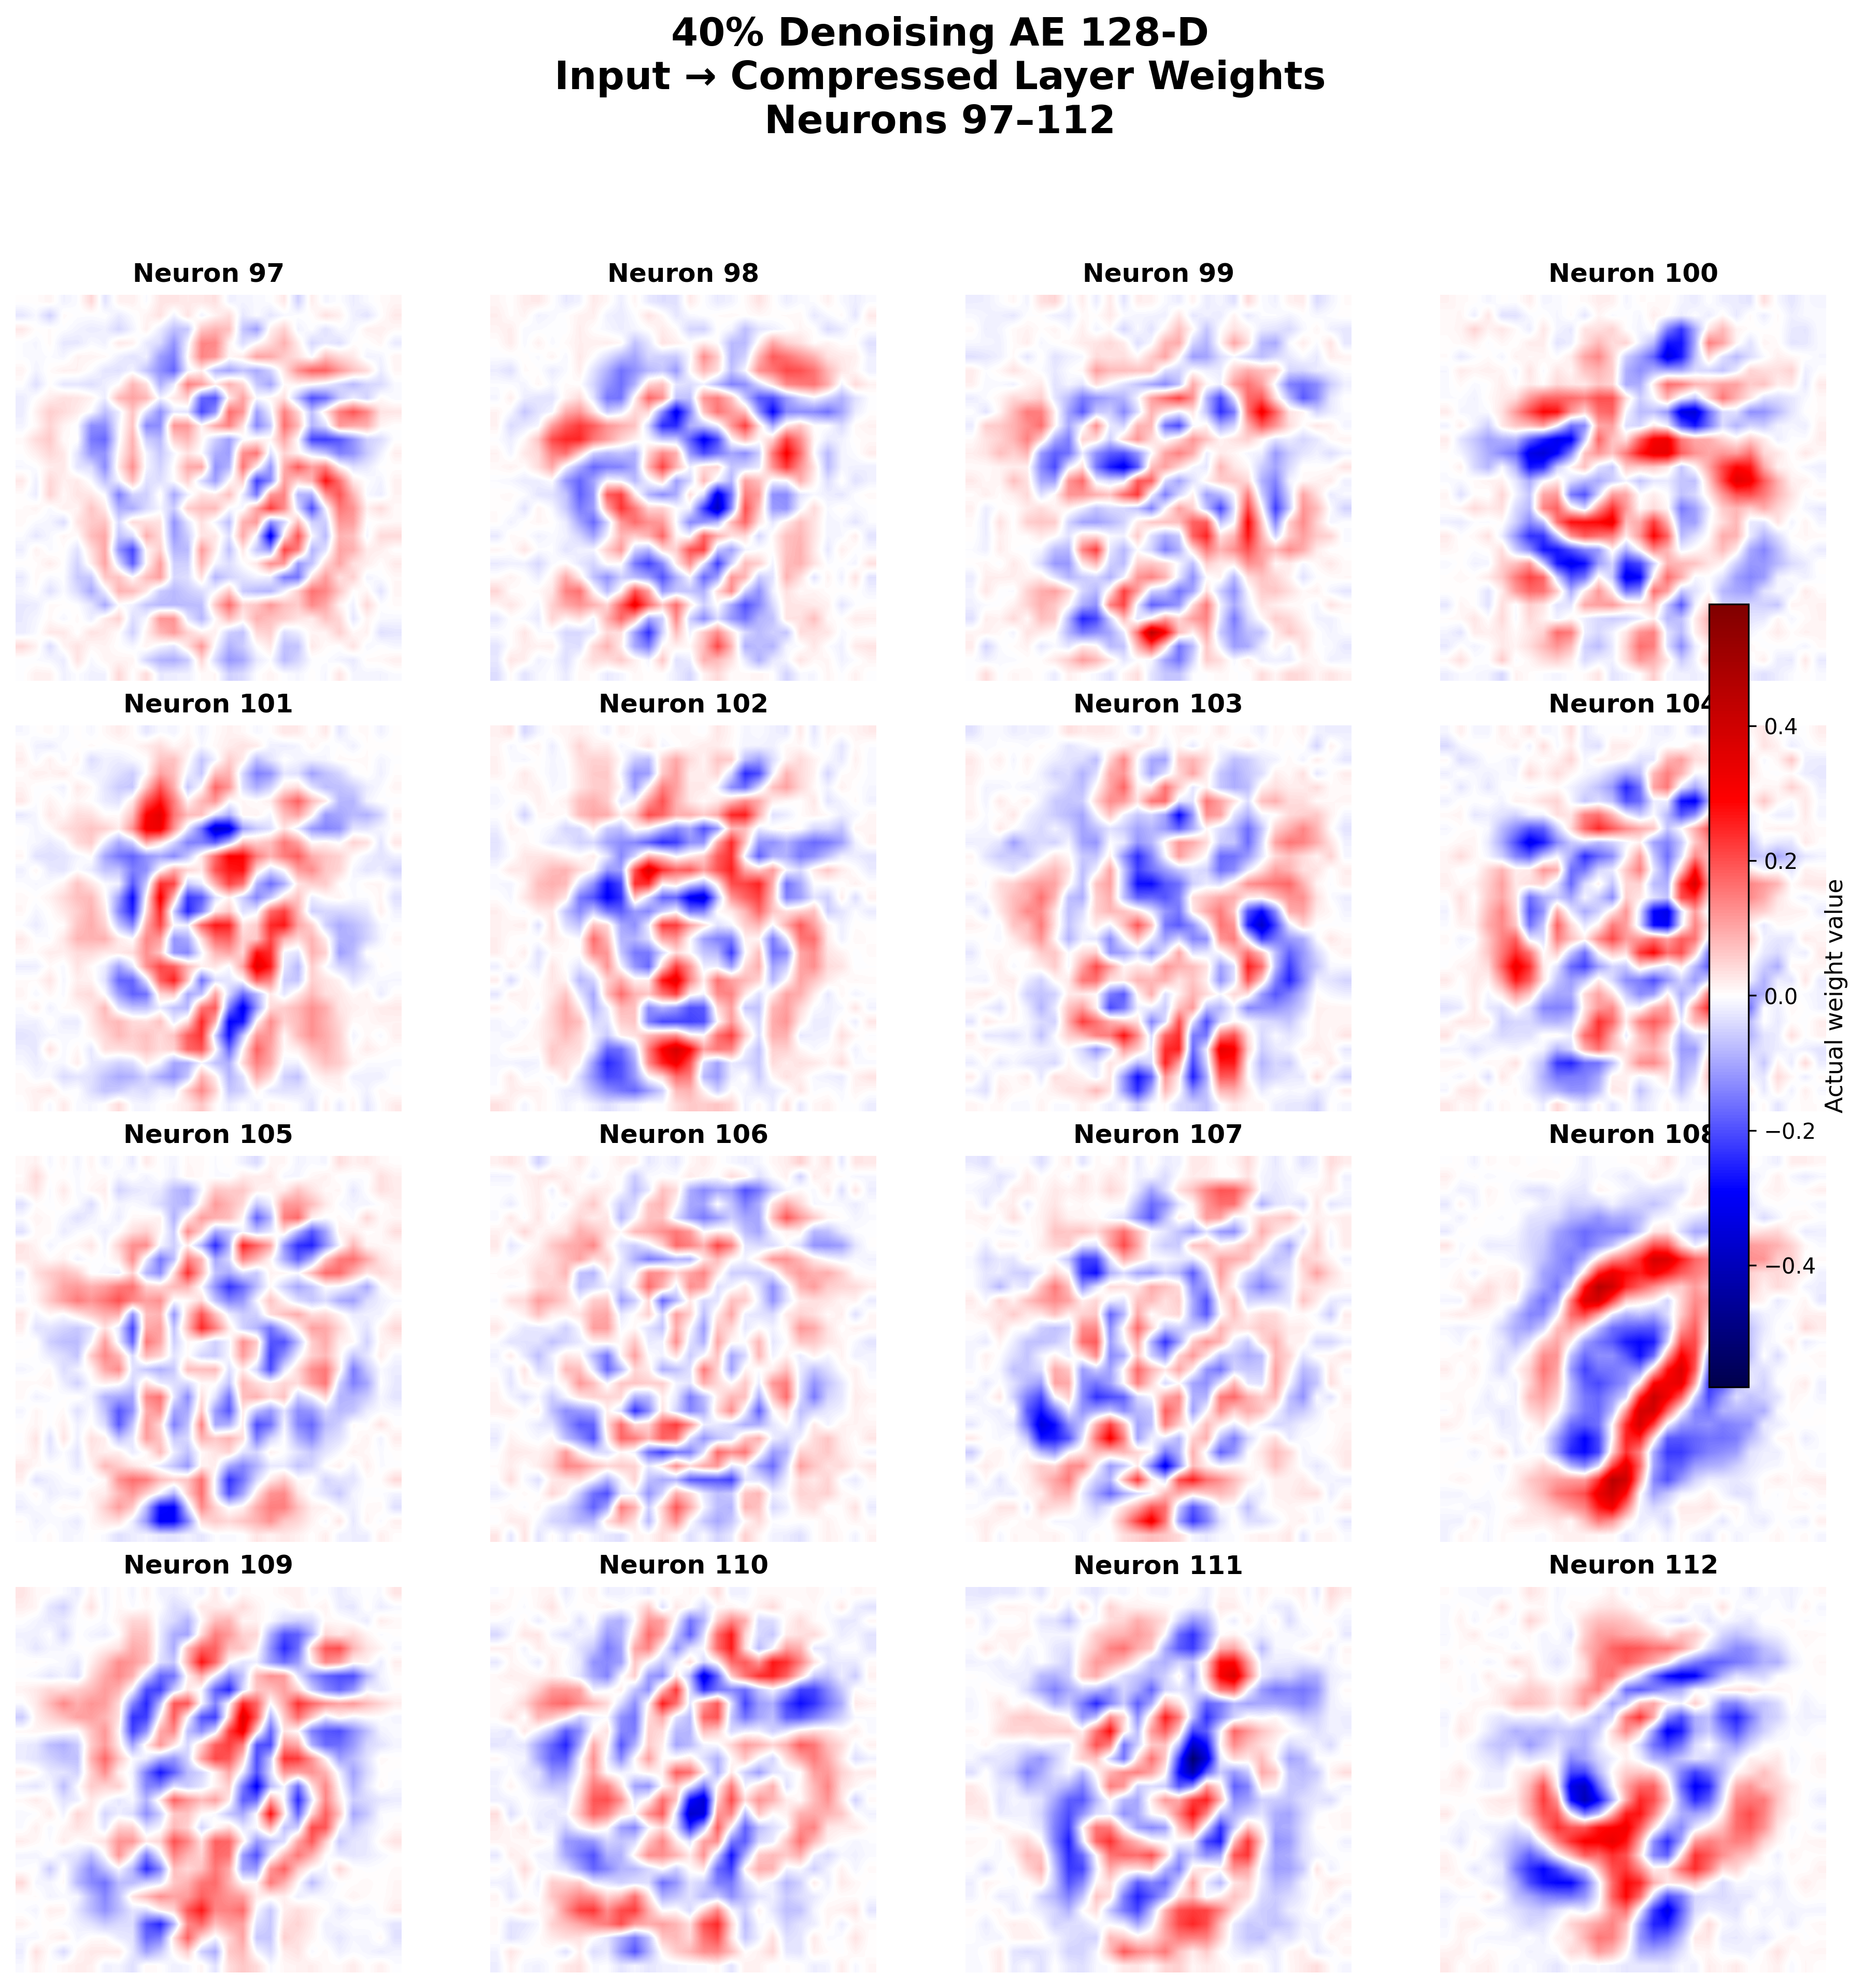
\includegraphics[width=0.99\linewidth,height=0.72\textheight,keepaspectratio]{figures/task6/40_pct_dae/neurons_097_112.png}
\caption{Input-to-bottleneck weight visualization for neurons 97--112.}
\label{fig:task6_23}
\end{figure}

\begin{figure}[H]
\centering
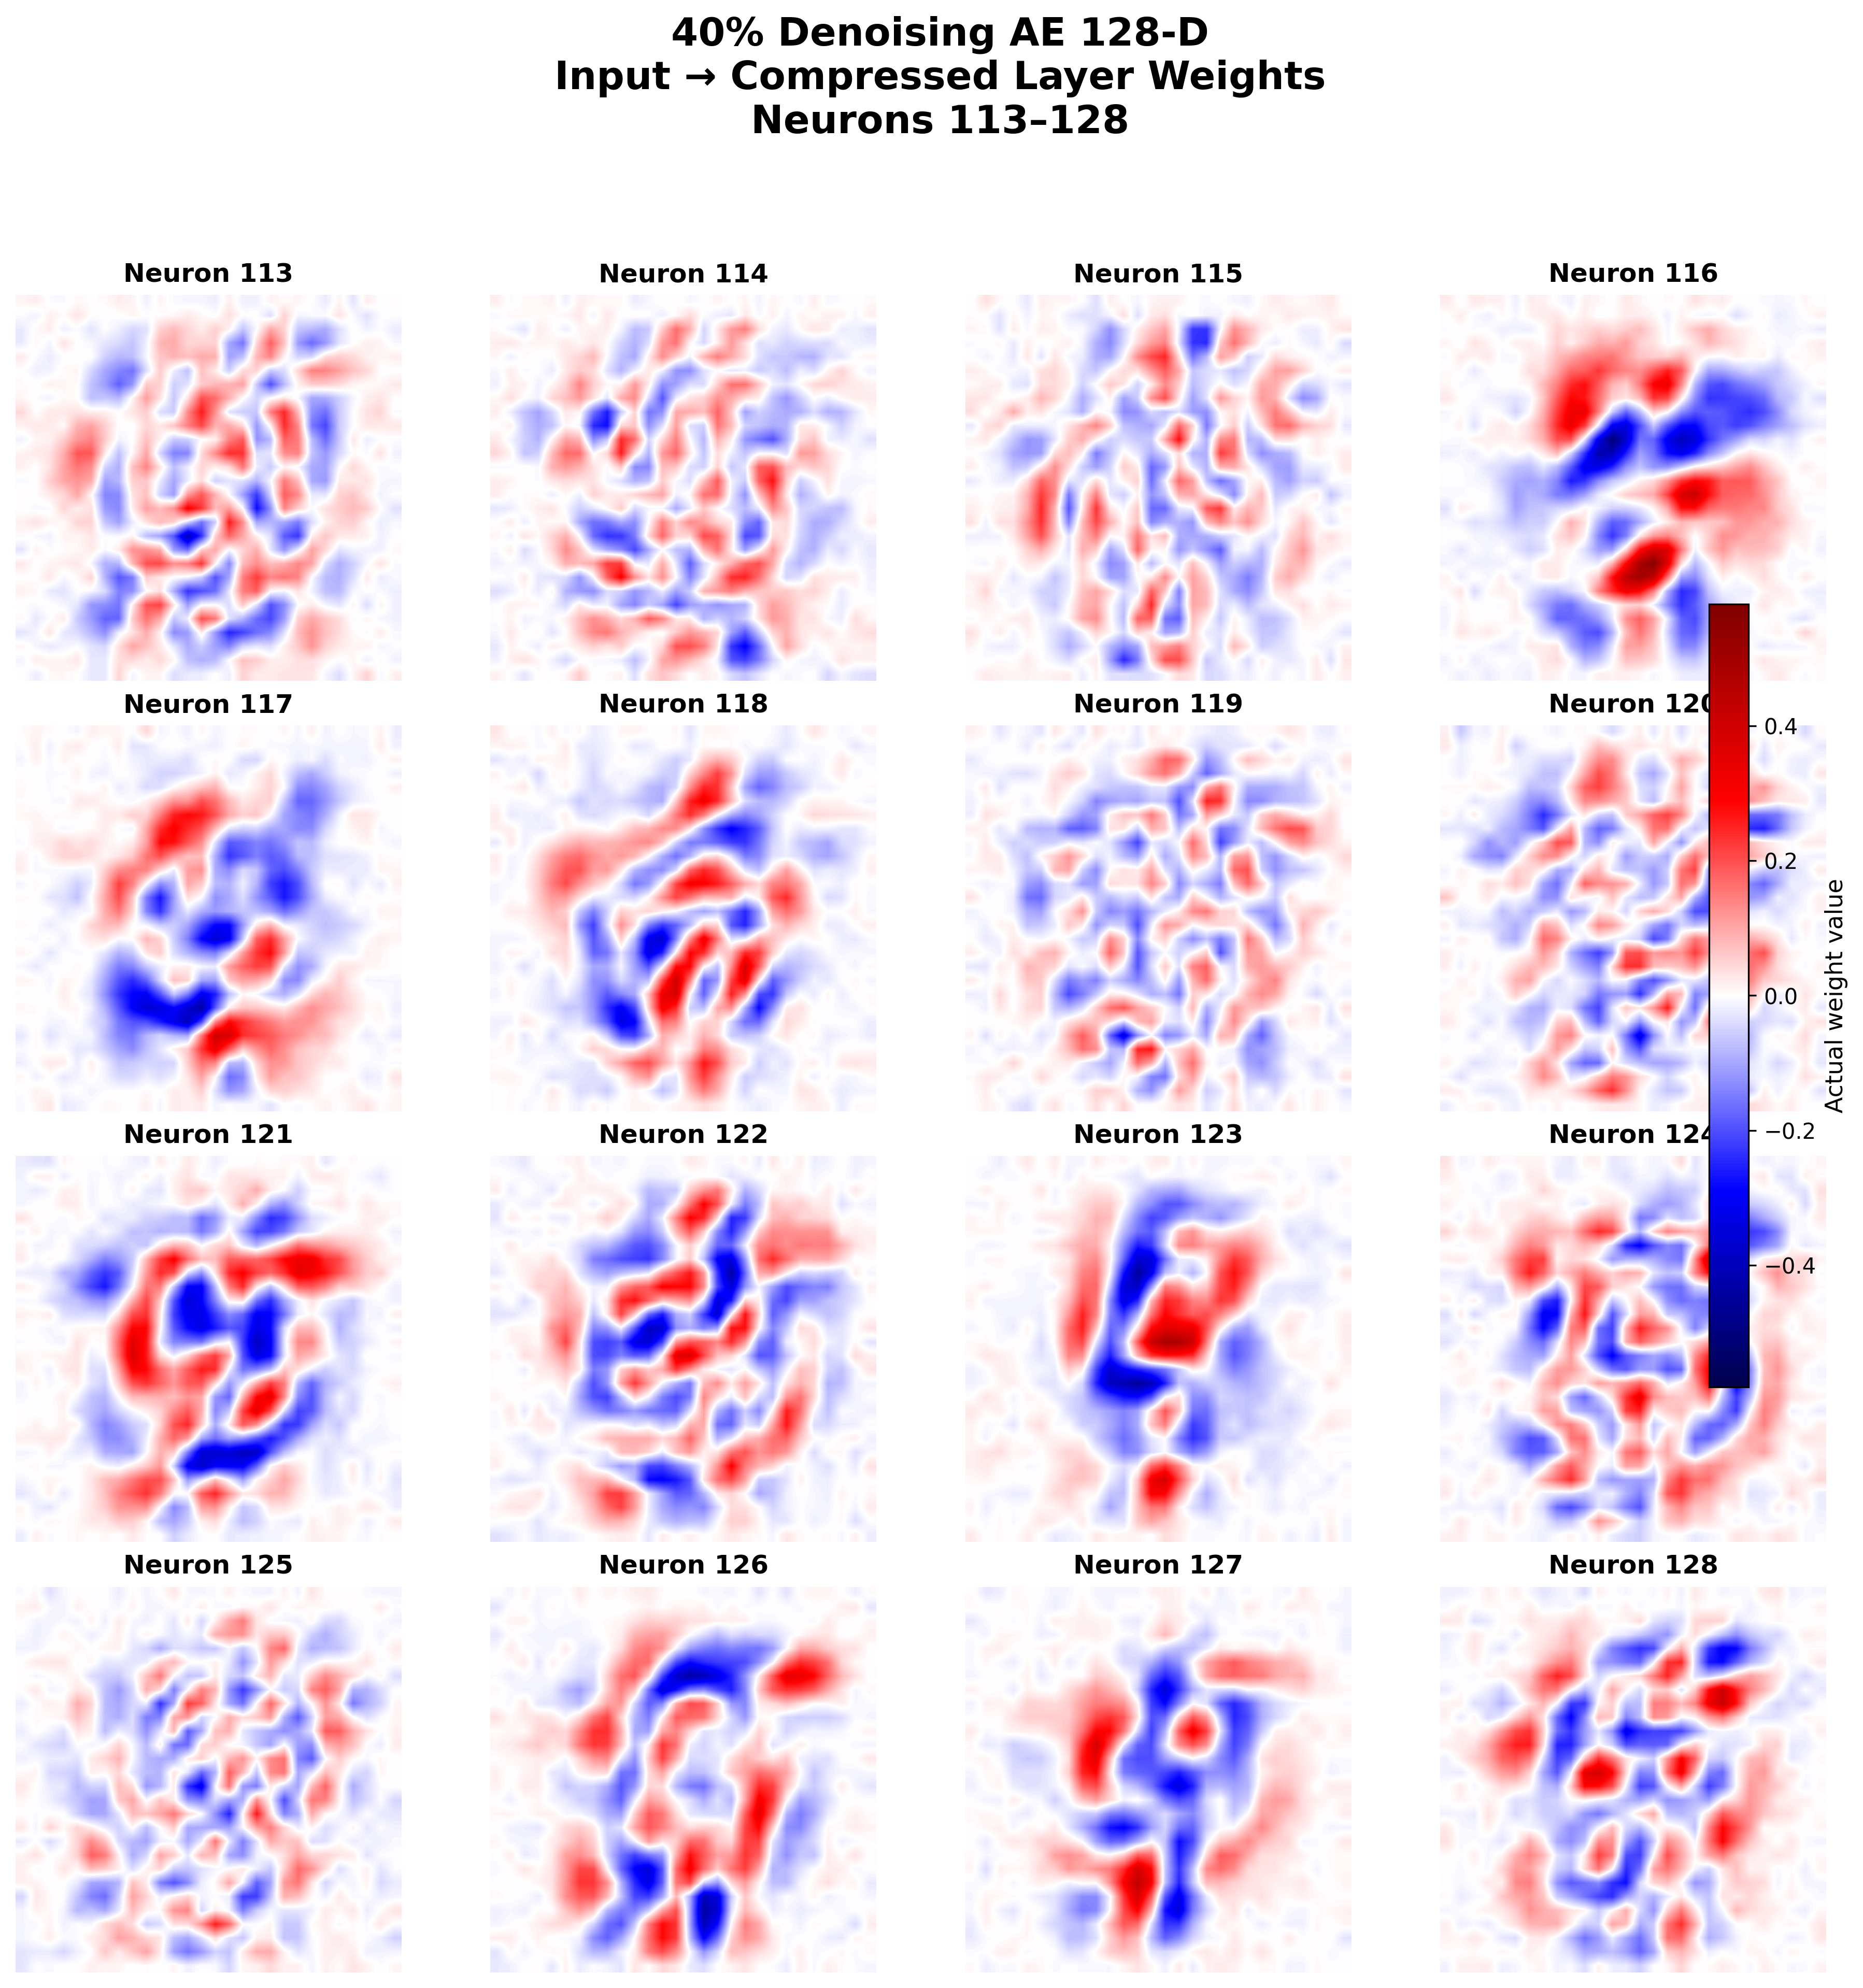
\includegraphics[width=0.99\linewidth,height=0.72\textheight,keepaspectratio]{figures/task6/40_pct_dae/neurons_113_128.png}
\caption{Input-to-bottleneck weight visualization for neurons 113--128.}
\label{fig:task6_24}
\end{figure}

\FloatBarrier

\section{Overall Comparison and Discussion}
Table~\ref{tab:overall} compares the best test results from Tasks 1, 3, 4, and 5 with the Assignment 3 baseline. Among the reported Assignment 4 classification experiments, the 20\% DAE gives the highest test accuracy at 98.4453\%, followed by the three-hidden-layer AE encoder at 64 dimensions with 98.2872\%. PCA reaches 98.2345\% at both 64 and 128 dimensions. The one-hidden-layer AE representation reaches 98.1555\% at 128 dimensions.

\begin{table}[H]
\centering
\caption{Overall best test classification results.}
\label{tab:overall}
\begin{tabular}{l r r}
\toprule
Method & Best representation & Test acc. (\%)\\
\midrule
Assignment 3 FCNN baseline & 784-D input & 98.1291\\
Task 1: PCA + FCNN & 64-D / 128-D & 98.2345\\
Task 3: One-hidden AE + FCNN & 128-D & 98.1555\\
Task 4: Three-hidden AE encoder + FCNN & 64-D & 98.2872\\
Task 5: 20\% DAE + FCNN & 128-D & 98.4453\\
Task 5: 40\% DAE + FCNN & 128-D & 98.4190\\
\bottomrule
\end{tabular}
\end{table}

These results support three cautious observations. First, dimensionality reduction can retain enough information for strong classification while reducing the input size substantially. Second, the latent dimension that minimizes reconstruction error is not necessarily the dimension that maximizes classification accuracy, because reconstruction and classification optimize different objectives. Third, in the denoising comparison, 20\% corruption outperforms 40\% corruption on both reconstruction MSE and downstream classification accuracy. These conclusions apply to the tested configurations and should not be generalized beyond the experimental setup without further experiments.

\section{Conclusion}
This assignment compared PCA features, conventional autoencoder, and denoising autoencoder representations for five-class handwritten-digit classification. PCA achieved 98.2345\% test accuracy at both 64 and 128 dimensions. The best one-hidden-layer AE representation reached 98.1555\%, while the best three-hidden-layer encoder representation reached 98.2872\%. The 20\% DAE achieved the strongest reported Assignment 4 classification accuracy, 98.4453\%, and also reconstructed better than the 40\% DAE according to test MSE. The reconstruction examples and weight visualizations provide qualitative complements to the quantitative metrics.

\begin{thebibliography}{9}
\bibitem{assignment3}
CS601T: Deep Learning, ``Programming Assignment 3,'' Department of Computer Science and Engineering, Indian Institute of Technology Dharwad, 2026.
\bibitem{lecture-notes}
CS601T: Deep Learning, ``Autoencoders,'' Course Lecture Notes, Department of Computer Science and Engineering, Indian Institute of Technology Dharwad, 2026.
\end{thebibliography}

\end{document}
